%%%%%%%%%%%%%%%%%%%%%%%%%%%%%%%%%%%%%%%%%
%%            LMU-Vorlage              %%
%%                                     %%
%%         zur Erstellung einer        %%
%%   Dissertation mit pdflatex/latex   %%
%%                                     %%
%%  (2002) Robert Dahlke               %%
%%         & Sigmund Stintzing         %%
%%%%%%%%%%%%%%%%%%%%%%%%%%%%%%%%%%%%%%%%%

\documentclass[12pt]{scrbook}

%%%%%%%%%%%%%%%%%%%%%%%%%%%%
%%   Zusaetzliche Pakete  %%
%%%%%%%%%%%%%%%%%%%%%%%%%%%%

\usepackage[utf8]{inputenc}
\usepackage[T1]{fontenc}
\usepackage{a4wide}
\usepackage{fancyhdr}
\usepackage{graphicx}
\usepackage[ngerman, english]{babel}
\usepackage{url}
\usepackage{natbib}
\usepackage[nottoc,numbib]{tocbibind}
\usepackage{paralist}

\usepackage{amsmath}
\usepackage{amsfonts}
\usepackage{amssymb}
\usepackage{bm}


\usepackage[bookmarks]{hyperref}


%%%%%%%%%%%%%%%%%%%%%%%%%%%%%%
%% Definition der Kopfzeile %%
%%%%%%%%%%%%%%%%%%%%%%%%%%%%%%

\pagestyle{fancyplain}
\renewcommand{\chaptermark}[1]%
         {\markboth{\thechapter.\ #1}{}}
\renewcommand{\sectionmark}[1]%
         {\markright{\thesection\ #1}}
\lhead[\fancyplain{}{\bfseries\thepage}]%
    {\fancyplain{}{\bfseries\rightmark}}
\rhead[\fancyplain{}{\bfseries\leftmark}]%
    {\fancyplain{}{\bfseries\thepage}}
\cfoot{}


%%%%%%%%%%%%%%%%%%%%%%%%%%%%%%%%%%%%%%%%%%%%%%%%%%%%%
%%  Definition des Deckblattes und der Titelseite  %%
%%%%%%%%%%%%%%%%%%%%%%%%%%%%%%%%%%%%%%%%%%%%%%%%%%%%%

\newcommand{\LMUTitle}[9]{
  \thispagestyle{empty}
  \vspace*{\stretch{1}}
  {\parindent0cm
   \rule{\linewidth}{.7ex}}
  \begin{flushright}

    \vspace*{\stretch{1}}
    \sffamily\bfseries\Huge
    #1\\
    \vspace*{\stretch{1}}
    \sffamily\bfseries\large
    #2
    \vspace*{\stretch{1}}
  \end{flushright}
  \rule{\linewidth}{.7ex}
  \vspace*{\stretch{5}}
  \begin{center}
    \includegraphics[width=2in]{siegel}
  \end{center}
  \vspace*{\stretch{1}}
  \begin{center}\sffamily\LARGE{#5}\end{center}
  \newpage
  \thispagestyle{empty}

  \cleardoublepage
  \thispagestyle{empty}

  \vspace*{\stretch{1}}
  {\parindent0cm
  \rule{\linewidth}{.7ex}}
  \begin{flushright}
    \vspace*{\stretch{1}}
    \sffamily\bfseries\Huge
    #1\\
    \vspace*{\stretch{1}}
    \sffamily\bfseries\large
    #2
    \vspace*{\stretch{1}}
  \end{flushright}
  \rule{\linewidth}{.7ex}

  \vspace*{\stretch{3}}
  \selectlanguage{ngerman}
  \begin{center}
    \Large Dissertation\\
    \Large an der #4\\
    \Large der Ludwig--Maximilians--Universit\"at\\
    \Large M\"unchen\\
    \vspace*{\stretch{1}}
    \Large vorgelegt von\\
    \Large #2\\
    \Large geboren am 26.06.~1979 in #3\\
    \vspace*{\stretch{2}}
    \Large M\"unchen, den #6
  \end{center}

  \newpage
  \thispagestyle{empty}

  \vspace*{\stretch{1}}

  \begin{flushleft}
    \large Erstgutachter:  #7 \\[1mm]
    \large Zweitgutachter: #8 \\[1mm]
    \large Tag der m\"undlichen Pr\"ufung: #9\\
  \end{flushleft}
  \selectlanguage{english}

  \cleardoublepage
}

%%%%%%%%%%%%%%%%%%%%%%%%%%%%%%%%%%%%%%%%%
%% Definitions & shortcuts for thesis  %%
%%%%%%%%%%%%%%%%%%%%%%%%%%%%%%%%%%%%%%%%%

\def\pdc{prior-data conflict}

\newcommand{\reals}{\mathbb{R}}

\newcommand{\dd}{\,\mathrm{d}}

\newcommand{\mbf}[1]{\mathbf{#1}}
\def\bs#1{\boldsymbol{#1}}

\newcommand{\X}{\mbf{X}}
\newcommand{\x}{\mbf{x}}

\newcommand{\uz}{^{(0)}} % upper zero
\newcommand{\un}{^{(n)}} % upper n

\def\yz{y\uz}
\def\yn{y\un}

\def\yzl{\ul{y}\uz}
\def\yzu{\ol{y}\uz}

\def\ynl{\ul{y}\un}
\def\ynu{\ol{y}\un}

\def\nz{n\uz}
\def\no{n\uo}
\def\nn{n\un}

\def\nzl{\ul{n}\uz}
\def\nzu{\ol{n}\uz}

\def\nnl{\ul{n}\un}
\def\nnu{\ol{n}\un}

\def\taux{\tau(x)}
\def\ttau{\tilde{\tau}}
\def\ttaux{\ttau(x)}

\def\Y{\mathcal{Y}}
\def\YZ{\Y\uz}
\def\YN{\Y\un}
\def\N{\mathcal{N}}
\def\NZ{\N\uz}
\def\NN{\N\un}
\def\PZ{\text{I}\!\Pi\uz}
%\def\PZero{\PZ}
\def\PN{\text{I}\!\Pi\un}
\def\MZ{\mathcal{M}\uz}
\def\MN{\mathcal{M}\un}

\newcommand{\p}{\operatorname{P}}
\newcommand{\E}{\operatorname{E}}
\newcommand{\V}{\operatorname{Var}}
\newcommand{\med}{\operatorname{med}} % Median
\newcommand{\mode}{\operatorname{mode}} % Mode
\newcommand{\logit}{\operatorname{logit}} % Mode

\def\El{\ul{\E}}
\def\Eu{\ol{\E}}

\def\Pl{\ul{\p}}
\def\Pu{\ol{\p}}

\newcommand{\mult}{\operatorname{M}}    % Multinomial Distribution
\newcommand{\norm}{\operatorname{N}}    % Normal Distribution
\newcommand{\ber}{\operatorname{Ber}}   % Bernoulli Distribution
\newcommand{\bin}{\operatorname{Binom}} % Binomial Distribution
\newcommand{\be}{\operatorname{Beta}}   % Beta Distribution
\newcommand{\B}{\operatorname{B}}   % Beta Function

% definitions only for thesis

\newtheorem{theorem}{Theorem}[chapter]
\newtheorem{definition}{Definition}[chapter]
\newtheorem{remark}{Remark}[chapter]
\newtheorem{example}{Example}[chapter]



%\includeonly{setsofconjugatepriors,alternatives} %
%\includeonly{appendix2}
%\includeonly{luck}

\hypersetup {
pdftitle = {Generalized Bayesian Inference under Prior-Data Conflict},
pdfauthor = {Gero Walter}
}

%%%%%%%%%%%%%%%%%%%%%%%%%%%%
%%  Beginn des Dokuments  %%
%%%%%%%%%%%%%%%%%%%%%%%%%%%%

\begin{document}


  \frontmatter


  \LMUTitle
      {Generalized Bayesian Inference\\ under Prior-Data Conflict}         % Titel der Arbeit
      {Gero Walter}                            % Vor- und Nachname des Autors
      {T\"ubingen}                             % Geburtsort des Autors
      {Fakult\"at f\"ur Mathematik, Informatik und Statistik} % Name der Fakultaet
      {M\"unchen 2013}                         % Ort und Jahr der Erstellung
      {14.08.~2013}                              % Tag der Abgabe
      {Prof.\ Dr.\ Thomas Augustin}            % Name des Erstgutachters
      {Prof.\ Dr.\ Frank P.A.\ Coolen}         % Name des Zweitgutachters
      {25.10.~2013}                            % Datum der muendlichen Pruefung

  \addcontentsline{toc}{chapter}{\protect Danksagung}


\chapter*{Danksagung}

Ich möchte allen einen Dank aussprechen,
die mich in der Zeit der Entstehung dieser Dissertation begleitet haben.
%
Thomas Augustin möchte ich herzlichen danken für die enge Zusammenarbeit,
für Enthusiasmus und Ermutigungen, und ganz besonders dafür, dass er
trotz der arbeitsintensiven administrativen Zumutungen, die über uns hereingebrochen sind,
immer für mich Zeit gefunden hat.
%
Frank Coolen möchte ich für seine Einladungen nach Durham und die spannende und inspirierende Zusammenarbeit danken.
%
Meinen Koautoren Matthias Troffaes und Manuel Eugster für alle Hilfe und die fruchtbare Zusammenarbeit.

Kollegen am Institut dafür mit den Problemem nicht allein zu sein
Büronachbarn dafür, mein gelegentliches Grummeln zu ertragen

BM, EH, CJ, die wie die anderen Mitarbeiter dafür gesorgt haben,
dass ich mich am Institut für Statistik wie zuhause fühlen konnte.

Familie

Mirjam


  \tableofcontents
  \addcontentsline{toc}{chapter}{\protect Contents}
  \markboth{Contents}{Contents}

  \listoffigures
  \addcontentsline{toc}{chapter}{\protect List of Figures}
  \markboth{List of Figures}{List of Figures}

  \listoftables
  \addcontentsline{toc}{chapter}{\protect List of Tables}
  \markboth{List of Tables}{List of Tables}
  \cleardoublepage

  \markboth{Abstract}{Abstract}
  \chapter*{Abstract}
\addcontentsline{toc}{chapter}{\protect Abstract}

This thesis is concerned with the generalisation of Bayesian inference towards the use of imprecise or interval probability,
with a focus on model behaviour in case of prior-data conflict.

Bayesian inference is one of the main approaches to statistical inference.
It requires to express (subjective) knowledge on the parameter(s) of interest not incorporated in the data by a so-called prior distribution.
All inferences are then based on the so-called posterior distribution,
the subsumption of prior knowledge and the information in the data calculated via Bayes' Rule.

The adequate choice of priors has always been an intensive matter of debate in the Bayesian literature.
While a considerable part of the literature is concerned with so-called non-informative priors
aiming to eliminate (or, at least, to standardise) the influence of priors on posterior inferences,
inclusion of specific prior information into the model may be necessary if data are scarce,
or do not contain much information about the parameter(s) of interest;
also, shrinkage estimators, common in frequentist approaches, can be considered as Bayesian estimators based on informative priors.

When substantial information is used to elicit the prior distribution through, e.g, an expert's assessment,
and the sample size is not large enough to eliminate the influence of the prior, \emph{prior-data conflict} can occur,
i.e., information from outlier-free data suggests parameter values which are surprising from the viewpoint of prior information,
and it may not be clear whether the prior specifications or the integrity of the data collecting method
(the measurement procedure could, e.g., be systematically biased) should be questioned.
In any case, such a conflict should be reflected in the posterior, leading to very cautious inferences,
and most statisticians would thus expect to observe, e.g., wider credibility intervals for parameters in case of prior-data conflict.
However, at least when modelling is based on conjugate priors, prior-data conflict is in most cases completely averaged out,
giving a false certainty in posterior inferences.

%i.e., data may be observed that are very unlikely from the standpoint of the prior,
%with posterior inferences depending heavily on the prior specification.
%
%Unfortunately, it can not be taken for granted that the presence of a serious prior-data conflict is easily identified, or that it is reflected in the shape of the posterior.
%
%While approaches to identify the presence and seriousness of prior-data conflict have been proposed,
%a widely accepted strategy for the case of a non-ignorable prior-data conflict seems to be missing.
%
%This conflict should show up in posterior inferences, alerting the analyst and, e.g., lead to a revision of prior specifications.

Here, imprecise or interval probability methods offer sound strategies to counter this issue,
by mapping parameter uncertainty over \emph{sets} of priors resp.\ posteriors instead over single distributions.
This approach is supported by recent research in economics, risk analysis and artificial intelligence,
corroborating the multi-dimensional nature of uncertainty and concluding that standard probability theory
as founded on Kolmogorov's or de Finetti's framework may be too restrictive,
being appropriate only for describing one dimension, namely ideal stochastic phenomena.

The thesis studies how to efficiently describe sets of priors in the setting of samples from an exponential family. 
Models are developed that offer enough flexibility to express a wide range of (partial) prior information,
give reasonably cautious inferences in case of prior-data conflict while resulting in more precise inferences when prior and data agree well,
and still remain easily tractable in order to be useful for statistical practice.
Applications in various areas, e.g.\ common-cause failure modeling and Bayesian linear regression, are explored,
and the developed approach is compared to other imprecise probability models.


  \markboth{Zusammenfassung}{Zusammenfassung}
  \selectlanguage{ngerman}
\chapter*{Zusammenfassung}
\addcontentsline{toc}{chapter}{\protect Zusammenfassung}

Das Thema dieser Dissertation ist die Generalisierung der Bayes-Inferenz
durch die Verwendung von unscharfen oder intervallwertigen Wahrscheinlichkeiten.
Ein besonderer Fokus liegt dabei auf dem Modellverhalten für den Fall,
dass Priori-Verteilung und Daten in Konflikt stehen.

Die Bayes-Inferenz ist einer der Hauptansätze zur Herleitung von statistischen Inferenzmethoden.
In diesem Ansatz muss (eventuell subjektives) Vorwissen über die Modellparameter,
welches nicht von den Daten erfasst wird, in einer sogenannten Priori-Verteilung (kurz: Priori) erfasst werden.
Alle Inferenzaussagen basieren dann auf der sogenannten Posteriori-Verteilung (kurz: Posteriori),
welche mittels des Satz' von Bayes berechnet wird, 
und das Vorwissen und die Informationen in den Daten zusammenfasst.

Wie eine Priori-Verteilung in der Praxis zu wählen sei, ist dabei stark umstritten.
Ein großer Teil der Literatur befasst sich mit der Bestimmung von sogenannten
nichtinformativen Prioris. Diese zielen darauf ab, den Einfluss der Priori auf die Posteriori
zu eliminieren oder zumindest zu standardisieren.
Falls jedoch nur wenige Daten zur Verfügung stehen, oder diese nur wenige Informationen
in Bezug auf die Modellparameter bereitstellen,
kann es hingegen nötig sein, spezifische Priori-Informationen in ein Modell einzubeziehen.
Außerdem können sogenannte Shrinkage-Schätzer, die in frequentistischen Ansätzen häufig zum Einsatz kommen,
als Bayes-Schätzer mit informativen Prioris angesehen werden.

Wenn spezifisches Vorwissen zur Bestimmung einer Priori genutzt wird (beispielsweise durch eine Befragung eines Experten),
und aber die Stichprobengröße nicht ausreicht, um eine solche informative Priori zu überstimmen,
kann sich ein Konflikt zwischen Priori und Daten ergeben.
Dieser kann sich darin äußern, dass die beobachtete (und von eventuellen Ausreißern bereinigte)
Stichprobe Parameterwerte impliziert, die aus Sicht der Priori äußerst überraschend und unerwartet sind.
In solch einem Fall kann es unklar sein, ob eher das Vorwissen oder eher die Validität der
Datenerhebung in Zweifel gezogen werden sollen.
(Es könnten beispielsweise Messfehler, Kodierfehler, oder eine Stichprobenverzerrung durch \emph{selection bias} vorliegen.)
%(Ein bestimmtes Messverfahren könnte beispielsweise zu systematischen Verzerrungen führen.)
Zweifellos sollte sich ein solcher Konflikt in der Posteriori widerspiegeln
und eher vorsichtige Inferenzaussagen bedingen;
die meisten Statistiker würden daher davon ausgehen,
dass sich in solchen Fällen breitere Posteriori-Kredibilitätsintervalle für die Modellparameter ergeben.
Bei Modellen, die auf konjugierten Prioris basieren,
wird ein solcher Konflikt jedoch einfach ausgemittelt.
Dann werden Inferenzaussagen, die auf einer solchen Posteriori basieren, den Anwender in falscher Sicherheit wiegen.

In dieser problematischen Situation können Intervallwahrscheinlichkeits-Methoden einen
fundierten Ausweg bieten, indem Unsicherheit über die Modellparameter mittels
\emph{Mengen} von Prioris beziehungsweise Posterioris ausgedrückt wird.
Neuere Erkenntnisse aus Risikoforschung, Ökonometrie und der Forschung zu künstlicher Intelligenz,
die die Existenz von verschiedenen Arten von Unsicherheit nahelegen,
unterstützen einen solchen Modellansatz,
der auf der Feststellung aufbaut, dass die auf den
auf den Ansätzen von Kolmogorov oder de Finetti basierende
übliche Wahrscheinlichkeitsrechung zu restriktiv ist,
um diesen mehrdimensionalen Charakter von Unsicherheit adäquat einzubeziehen,
und sich stattdessen nur auf eine der Dimensionen beziehen kann,
nämlich die der idealen Stochastizität.

In dieser Dissertation wird untersucht, wie sich Mengen von Prioris
für Stichproben aus Exponentialfamilien effizient beschreiben lassen.
Wir entwickeln Modelle, die eine ausreichende Flexibilität gewährleisten,
so dass eine Vielfalt von Ausprägungen von partiellem Vorwissen beschrieben werden kann.
Diese Modelle führen zu vorsichtigen Inferenzaussagen,
wenn ein Konflikt zwischen Priori und Daten besteht,
und ermöglichen dennoch präzisere Aussagen für den Fall, dass Priori und Daten im Wesentlichen übereinstimmen,
ohne die Einsatzmöglichkeiten in der statistischen Praxis durch
eine zu hohe Komplexität in der Anwendung zu erschweren.
Anwendungen in verschiedenen Bereichen, unter anderem in sogenannten
common-cause-failure-Modellen und in der linearen Bayes-Regression,
werden untersucht, 
und das in dieser Dissertation entwickelte Modell wird mit anderen Intervallwahrscheinlichkeits-Modellen verglichen.


%\selectlanguage{english}


\mainmatter\setcounter{page}{1}
  \chapter{Introduction}


\begin{itemize}
\item overview, which paper used where\ldots
\item statistical inference ??? (\textbf{StatInf chapter}, \cite{itip-statinf})
\item Bayesian inference, conjugate priors, etc. (\textbf{TechRep Dirichlet}, \cite{Walter2012b})
\item motivate priors etc.\ with ress paper: \cite{Walter2013a}
\item short part on decision theory, updating rules?
\item \pdc\ (Evans \& Moshonov), examples (\textbf{Festschrift paper}, \cite{Walter2010a})
\item other motivations for IP?
\end{itemize}

\section{Overview}

***structure, which papers where***

Sec.~\ref{sec:stat-inference}: parts of \cite{itip-statinf}

Sec.~\ref{sec:bayes-inference}: parts of \cite{itip-statinf}

Sec.~\ref{sec:inferencetasks}: parts of \cite{itip-statinf}

Sec.~\ref{sec:beta-binom}: parts of \cite{itip-statinf}

\section{Statistical Inference}
\label{sec:stat-inference}

%This thesis being concerned with generalized Bayesian Inference

In this Section, we will give a short introduction to statistical inference
and models that are used to describe random samples.
%These introductory sections may also serve as a guide to the notation utilized.

Statistical inference is about learning from data.
It is basically concerned with inductive reasoning,
i.e.\ establishing a general rule from observations.
As is long known as the problem of induction \cite{1739:hume},
it is impossible to justify inductive reasoning by pure reason,
and therefore one cannot infer general statements (laws) with absolute truth from single observations.
%***statistical models are built for a certain purpose. (citexxx George P. Box, Kaplan?)\\
%***models try to mirror certain aspects of reality: those deemed relevant to answer %the question(s) at hand etc.
The statistical remedy for this inevitable and fundamental dilemma of any type of inductive reasoning is
(postulated, maybe virtual) \emph{randomness} of the sampling process that generates the data.
If, and only if, the sample is, or can be understood as, drawn randomly,
probability theory allows to quantify the error of statistical propositions concluded from the sample.

Specifically, to model the randomness, a \emph{statistical model} is formulated.
It is a tuple $(\mathcal{X}, \mathcal{Q})$, consisting of the \emph{sample space} $\mathcal{X}$,
i.e.\ the domain of the random quantity $X$ under consideration,
and a set $\mathcal{Q}$ of probability distributions,%
\footnote{Most models of statistical inference rely on $\sigma$-additive probability distributions.
Therefore, technically, in addition an appropriate ($\sigma$-)field $\sigma(\mathcal{X})$,
describing the domain of the underlying probability measure, has to be specified.
In most applications there are straightforward canonical choices for $\sigma(\mathcal{X})$,
and thus $\sigma$-fields are not explicitly discussed here.}
collecting all probability distributions that are judged to be potential candidates for the distribution of $X$.
In this setting $\mathcal{Q}$ is called \emph{sampling model} and every element $p\in \mathcal{Q}$ \emph{(potential) sampling distribution}.
The inferential task is to learn the true element $p^* \in \mathcal{Q}$ from multiple observations of the random process producing $X$.


\subsection{Parametric Models}
\label{sec:parametricmodels}

In this thesis, generally, so-called \emph{parameteric models} are considered,
where $\mathcal{Q}$ is pa\-ra\-me\-trized by a parameter $\vartheta$ of finite dimension,
assuming values in the so-called \emph{parameter space} $\Theta$, $\Theta \subseteq \reals^q, \ q < \infty$,
i.e.\ ${\cal Q}=\left(p_\vartheta\right)_{\vartheta \in \Theta}$.
Here, the different sampling distributions $p_\vartheta$ are implicitly understood as belonging to a specific class of distributions
(e.g. normal distributions, see the example in ****),
the basic type of which is assumed to be known completely,
and only some characteristics $\vartheta$ (e.g.\ the mean) of the distributions are unknown.

Throughout, we will assume (as is the case for all common applications)
that the underlying candidate distributions $p_\vartheta$ of the random quantity $X$
are either discrete or absolutely continuous with respect to the Lebesgue measure
(see, e.g. \cite[pp.~32f, 38]{1993:karr} for some technical details) for every $\vartheta \in \Theta$.
Then it is convenient to express every $p_\vartheta$ in the discrete case by its \emph{mass function} $f_\vartheta$,
with $f_\vartheta(x):=p_\vartheta(X=x),\forall x \in \mathcal{X}$,
and in the continuous case by its \emph{probability density function} (pdf) $f_\vartheta$,
where $f_\vartheta$ is such that $p_\vartheta(X \in [a,b]) = \int_a^b f_\vartheta(x) \dd x$.

An \emph{i.i.d.\ sample of size} $n$ (where \emph{i.i.d.}\ abbreviates independent, identically distributed)
\emph{based on the parametric statistical model} %
$(\mathcal{X}, (p_\vartheta)_{\vartheta \in \Theta})$ is a vector
\[
{\X}=(X_1, \ldots, X_n)^T %\label{120722-1}
\]
of independent random quantities $X_i$ with the same distribution $p_\vartheta$.
Then $\X$ is defined on $\mathcal{X}^n$ with probability distribution $p_\vartheta^{\otimes n}$
as the $n$-dimensional product measure describing the independent observations.
For Bayesian approaches as discussed here,
independence is often replaced by exchangeability (see, e.g., \cite[\S 4.2]{2000:bernardosmith}).
$p_\vartheta^{\otimes n}$ thus has the probability mass or density function
\[
\prod_{i=1}^{n} f_\vartheta(x_i) =: f_\vartheta(x_1, \ldots, x_n).%\label{120710-2}
\]
The term \emph{sample} is then also used for the concretely observed value(s) $\x=(x_1, \ldots, x_n)^T$.%
\footnote{Throughout, random quantities are denoted by capital letters, their values, or realizations, by small letters.}

Next, we will present two examples for basic parametric models that will be repeatedly discussed further on.


\subsection{The Normal Distribution}
\label{sec:normaldist}

A common model for observations that in principle can assume any value on the real line
is the \emph{normal distribution} with parameters $\mu$ and $\sigma^2$, also called the \emph{Gaussian distribution}.
Typical examples for data of this kind are scores in intelligence testing, or technical measurements in general.%
\footnote{The normal distribution is distinguished by the central limit theorem
(see, e.g., \cite[\S 7.3]{1993:karr}, or \cite[\S 9]{1968:breiman}), stating that, under regularity conditions,
the distribution of an appropriately scaled sum of $n$ standardized random variables converges to a normal distribution
for $n \longrightarrow \infty$.}

For each observation $x_i$, $i=1,\ldots, n$, the normal probability density is
\begin{align*}
f_{(\mu, \sigma^2)}(x_{i}) &= \frac{1}{\sqrt{2\pi\sigma^2}}\exp\Big\{ -\frac{1}{2\sigma^2}(x_{i} - \mu)^2 \Big\}\,,
\end{align*}
with the two parameters $\mu \in \reals$ and $\sigma^2 \in \reals_{>0}$
being in fact the mean and the variance of (the distribution of) $x_i$, respectively.
As a shortcut, we write $x_i \sim \norm(\mu, \sigma^2)$.
%a normal density with $\mu=0$ and $\sigma^2=1$ is displayed
%in Figure~\ref{inference:fig:normal-vs-cauchy}, page~\pageref{inference:fig:normal-vs-cauchy}.

With the independence assumption, the density of $\mbf{x} = (x_1,\ldots,x_n)$ amounts to
\begin{align}\label{eq:normaldens}
f_{(\mu, \sigma^2)}(\mbf{x})
 &= \prod_{i=1}^n f_{(\mu, \sigma^2)}(x_{i})
  = (2\pi\sigma^2)^{-\frac{n}{2}}\exp\Big\{ -\frac{1}{2\sigma^2}\sum_{i=1}^n (x_{i} - \mu)^2 \Big\}\,.
\end{align}

Later on, we restrict considerations to the case where the variance $\sigma_0^2$ is known, denoted by $x_i \sim \norm(\mu, \sigma_0^2)$.
Inference may thus concern the parameter $\mu$ directly, or future observations $x_{n+1}, x_{n+2}, \ldots$ in a chain of i.i.d.\ observations.


\subsection{The Multinomial Distribution}
\label{sec:multinomdist}

The \emph{multinomial distribution} is a common model for samples where only a limited number of distinct values can be observed.
%like in the data from an election poll, or from a pharmacological study asking about a certain set of adverse reactions.
These distinct values are often named \emph{categories} (hence the term \emph{categorical data}),
and are usually numbered from $1$ to $k$, without imposing any natural ordering on these values.
We have therefore a discrete distribution,
giving the probability for observing certain category counts $(n_1, \ldots, n_k) = \mbf{n}$ in a sample of $n$ observations in total.
Thus, $\sum_{j=1}^k n_j = n$.

We start the definition of the multinomial distribution by decomposing the collection of $n$ observations into its constituents,
single observations of either of the categories $1,\ldots,k$.
Such a single observation, often named \emph{multivariate Bernoulli observation}, can be encoded as a vector $x_i$ of length $k$,
where the $j$-th element, $x_{ij}$, equals $1$ if category $j$ has been observed, and all other elements being $0$.
Given the vectorial parameter $\theta$ of length $k$,
where the component $\theta_j$ models the probability of observing category $j$ in a single draw
(therefore $\sum_{j=1}^k \theta_j = 1$),
the probability for observing $x_i$ can be written as
\begin{align*}
f_\theta(x_i) = \prod_{j=1}^k \theta_j^{x_{ij}}\,.
\end{align*}
Assuming independence, the probability for observing a certain sequence $\mbf{x}$ of $n$ observations can thus be written as
\begin{align*}
f_\theta(\mbf{x}) &= \prod_{i=1}^n f_\theta(x_i)
             \propto \prod_{i=1}^n \prod_{j=1}^k \theta_j^{x_{ij}}
                   = \prod_{j=1}^k \theta_j^{\sum_{i=1}^n x_{ij}}
                   = \prod_{j=1}^k \theta_j^{n_j}\,,
\end{align*}
where $n_j = \sum_{i=1}^n x_{ij}$ tells us how often category $j$ was observed in the sample.

For the probability to observe a certain category count $(n_1, \ldots, n_k) = \mbf{n}$,
we have to account for the different possible orderings in $\mbf{x}$ leading to the same count vector $\mbf{n}$.
Therefore,
\begin{align}\label{eq:multinomdens}
f_\theta(\mbf{n}) &= \binom{n}{n_1,\ldots,n_k} \prod_{j=1}^k \theta_j^{n_j}
                   = \frac{n!}{n_1!\cdot \ldots \cdot n_k!} \prod_{j=1}^k \theta_j^{n_j}\,.
%             \propto \prod_{j=1}^k \theta_j^{n_j}\,.
\end{align}
As a shortcut, we write $\mbf{n} \sim \mult(\theta)$.


\section{Statistical Inference with the Bayesian Paradigm}
\label{sec:bayes-inference}

As the inference models discussed in this thesis are all based on the Bayesian approach to statistical inference,
we will now give a short introduction to the basic principles of Bayesian inference.

The Bayesian approach allows (possibly subjective) knowledge on the parameter $\vartheta$ to be expressed by a probability distribution on%
\footnote{Again we implicitly assume that $\Theta$ is complemented by an appropriate $\sigma$-field $\sigma(\Theta)$.}
$\Theta$, with probability mass or density function $p(\vartheta)$ called \emph{prior distribution}.
Interpreting the elements $f_\vartheta(x)$ of the sampling model as conditional distributions of the sample given the parameter,
denoted by $f(\mbf{x}\mid\vartheta)$ and called \emph{likelihood},
turns the problem of statistical inference into a problem of probabilistic deduction,
where the \emph{posterior distribution}, i.e.\ the distribution of the parameter given the sample data,
can be calculated by Bayes' Rule.%
\footnote{Donald Gillies \cite{1987:gillies, 2000:gillies} argues that Bayes' Theorem was actually developed
in order to confront the problem of induction as posed by Hume \cite{1739:hume}.}
Thus, in the light of the sample $\mbf{x}= (x_1, \ldots, x_n)$ the prior distribution is updated by Bayes' Rule
to obtain the posterior distribution with density or mass function
\begin{align}
\label{eq:bayesrule}
p(\vartheta\mid\mbf{x}) \propto f(\mbf{x}\mid\vartheta) \cdot p(\vartheta)\,.
\end{align}
The posterior distribution is understood as comprising all the information from the sample and the prior knowledge.
It therefore underlies all further inferences on the parameter $\vartheta$,
like point estimators, interval estimators,
or the \emph{posterior predictive distribution},
which is the distribution of further observations based on $p(\vartheta\mid\mbf{x})$
(see Eq.~\eqref{eq:posteriorpredictive} below).


\subsection{Regular Conjugate Families of Distributions}

Traditional Bayesian inference is frequently based on so-called \emph{conjugate priors} related to a specific likelihood.
Such priors have the convenient property that the posterior resulting from~\eqref{eq:bayesrule}
belongs to the same class of parametric distributions as the prior, and thus only the parameters have to be updated,
which makes calculation of the posterior and thus the whole Bayesian inference easily tractable.

Fortunately, there are general results guiding the construction of conjugate priors in models used most frequently in practice,
namely in the case where the sample distribution belongs to a so-called \emph{(regular) canonical exponential family}
\cite[pp.~202 and 272f]{2000:bernardosmith}. %Def.~4.12 and Prop.~5.6
This indeed covers many sample distributions relevant in a statistician's everyday life,
like Normal and Multinomial models, Poisson models, or Exponential and Gamma models.
After presentation of the general framework, we will discuss its instantiation for the Normal
and the Multinomial sampling models as introduced in Sections~\ref{sec:normaldist} and \ref{sec:multinomdist} above.

A sample distribution
(from now on understood directly as the distribution $p_\vartheta^{\otimes n}$ of an i.i.d.\ sample $\mbf{x}$ of size $n$)
is said to belong to the \emph{(regular) canonical exponential family} if its density or mass function satisfies the decomposition
\begin{align}\label{eq:expofam-sampledens}
f(\x \mid \theta) &\propto \exp\big\{\langle \psi, \tau(\x) \rangle - n \mbf{b}(\psi)\big\}\,,
\end{align}
where $\psi \in \Psi \subset \reals^q$ is a transformation of the (possibly vectorial) parameter $\theta \in \Theta$,
and $\mbf{b}(\psi)$ a scalar function of $\psi$ (or, in turn, of $\theta$).
$\tau(\x)$ is a function of the sample $\x$ that fulfills $\tau(\x) = \sum_{i=1}^n \tau^*(x_i)$,
with $\tau^*(x_i) \in \mathcal{T} \subset \reals^q$,
while $\langle\cdot, \cdot\rangle$ denotes the scalar product.
From these ingredients, a conjugate prior on $\psi$ can be constructed as%
\footnote{In our notation, ${}\uz$ denotes prior parameters; ${}\un$ posterior parameters.}
\begin{align}\label{eq:canonicalprior}
p(\psi \mid \nz, \yz) \dd\psi
 &\propto \exp\Big\{ \nz \Big[ \langle \yz, \psi \rangle - \mbf{b}(\psi) \Big] \Big\} \dd\psi\,,
\end{align}
where $\nz$ and $\yz$ are now the parameters by which a certain prior can be specified.
The domain of $\yz$ is $\Y$, the interior of the convex hull of $\mathcal{T}$;
$\nz$ must take strictly positive values for the prior to be proper (integrable to $1$).

An interpretation for these parameters will be given shortly.
First, let us calculate the posterior density for $\psi$.
The prior parameters $\yz$ and $\nz$ are updated to their posterior values $\yn$ and $\nn$ in the following way:
\begin{align}\label{eq:canonicalupdate}
\yn &= \frac{\nz}{\nz + n} \cdot \yz + \frac{n}{\nz + n} \cdot \frac{\tau(\x)}{n}\,, &
\nn &= \nz + n\,,
\end{align}
such that the posterior can be written as
\begin{align}\label{eq:canonicalposterior}
p(\psi \mid \x, \nz, \yz)
 =: p(\psi \mid \nn, \yn)
 &\propto \exp\Big\{ \nn \Big[ \langle \yn, \psi \rangle - \mbf{b}(\psi) \Big] \Big\} \dd\psi\,.
\end{align}
In this setting, $\yz$ and $\yn$ can be seen as the parameter describing the main characteristics of the prior and the posterior,
and thus we will call them \emph{main prior} and \emph{main posterior parameter}, respectively.
$\yz$ can also be understood as a prior guess for the random quantity $\ttau(\x) := \tau(\x)/n$ summarizing the sample,
as $\E[\ttau(\x) \mid \psi] = \nabla\mbf{b}(\psi)$,
where in turn $\E[\nabla\mbf{b}(\psi) \mid \nz, \yz] = \yz$ \cite{2000:bernardosmith}***more concrete***.

Characteristically, $\yn$ is a weighted average of this prior guess $\yz$ and the sample `mean' $\ttau(\x)$,
with weights $\nz$ and $n$, respectively.%
\footnote{This weighted average property of Bayesian updating with conjugate priors is an important issue
we comment on ***later / in Section~\ref{}***.}
Therefore, $\nz$ can be seen as ``prior strength'' or ``pseudocounts'',
reflecting the weight one gives to the prior as compared to the sample size $n$.
To make this more explicit, $\nz$ can be interpreted as the size of an imaginary sample
that corresponds to the trust on the prior information in the same way
as the sample size of a real sample
corresponds to the trust in conclusions based on such a real sample \cite[p.~258]{Walter2009a}.

The posterior $p(\psi \mid \nn, \yn)$ can be transformed back to a distribution on $\theta$
in order to deal with a commonly known parameter or distribution family for it
(as we will do in Section~\ref{}*** below.)
Besides the posterior itself, also the posterior predictive distribution
\begin{align}
\label{eq:posteriorpredictive}
f(\x^*\mid\x) &= \int f(\x^* \mid \psi) p(\psi \mid \nn, \yn) \dd\psi\,,
\end{align}
a distribution on future samples $\x^*$ after having seen a sample $\x$,
forms the basis for the different inference tasks. %as listed in Section~\ref{inference:sec:basictasks}.
Next, we will thus briefly describe a systematic of inference tasks.


\subsection{Inference Tasks}
\label{sec:inferencetasks}

We may structure the different inference tasks by
the type of statement one wants to infer from the data.
As such, this systematic is not exclusive to Bayesian inference methods,
and neither to the parametric models considered in Section~\ref{sec:parametricmodels},
but it will be formulated in terms of parameters in a Bayesian setting here.

We distinguish two groups of inferences, namely
\begin{enumerate}
\item static conclusions and
\item predictive conclusions.%
%\footnote{Static conclusions are still more common in statistical applications.
%In the light of the success of procedures from machine learning in statistics, the predictive view,
%early propagated, e.g., by \cite{1993:geisser}, has attracted increasing attention.}
\end{enumerate}

\emph{Static conclusions} refer directly to properties of the sampling model, typically to its parameter(s).
The following procedures, which are based directly on the posterior \eqref{eq:canonicalposterior} in the Bayesian paradigm,
are the most common:
\begin{enumerate}
\item[1a)] \emph{Point estimators},
where a certain parameter value is selected to describe the sample.
\item[1b)] \emph{Interval estimators},
where the information is condensed in a certain subset of the parameter space $\Theta$, typically in an interval when $\Theta \subseteq \reals$.
\item[1c)] \emph{Hypotheses tests},
where the information in the sample is only used to decide between two mutually exclusive statements called \emph{hypotheses},
usually denoted by $H_0$ and $H_1$.
\item[1e)] \emph{Decision making},
where, more generally, the conclusion may be to select certain utility maximizing or loss minimizing acts from a set of possible acts.
Indeed, all three tasks listed before can be formally understood as a special case of decision making,
by considering an appropriate set of acts and a loss function fitting the inferential objective.
We will flesh this out to some extent in the examples below***.%
\footnote{For more details, see, e.g., ******.}
\end{enumerate}

\emph{Predictive conclusions} instead summarize the information by statements on properties of typical further units,
either by describing the whole distribution (as with the posterior predictive \eqref{eq:posteriorpredictive},
or by certain summary measures.
Similar to static conclusions, one can thus consider, e.g.,
\begin{enumerate}
\item[2a)] \emph{Point prediction},
where a certain sample value is selected as the most likely to occur.
This is especially useful in the case of discrete sampling distributions,
where this procedure amounts to classification of further sample units.
\item[2b)] \emph{Interval prediction},
where instead a certain subset of the sample space $\mathcal{X}$ is determined,
into which furter sample units are like to fall.
An example are prediction bands in regression analysis.
\end{enumerate}

The concretion of this framework for Bayesian inference with regular conjugate priors
is now demonstrated for the sampling models presented in Sections~\ref{sec:normaldist} and \ref{sec:multinomdist}.
As a first simple example, we will consider inference in the Binomial model,
being the special case of the Multinomial model with only two categories.
Then, we will briefly turn to the Normal model,
before we present the more complex considerations for the Multinomial model with $k>2$ categories.
The latter model %for the Multinomial model (Section~\ref{sec:multinomdist})
is then used for inferences in common-cause modeling,
which will serve as a real-world example illustrating the powers and shortcomings of standard Bayesian inference,
ultimately motivating the shift to imprecise Bayesian inference.


\subsection{The Beta-Binomial Model}
\label{sec:beta-binom}

As the special case of the multinomial model \eqref{eq:multinomdens} with only two categories, we will consider the Binomial model
\begin{align}
\label{eq:binomdens}
f(\x\mid\theta) &= {n \choose s}\theta^s (1-\theta)^{n-s}\,,
\end{align}
where $\x$, the vector of $n$ observations, is composed of scalar $x_i$'s being either $0$ or $1$
denoting `failure' or `success' in an experiment with these two outcomes.
$s = \sum_{i=1}^n x_i$ is the number of successes,
and the (unknown) parameter $\theta \in (0,1)$ is the probability for `success' in a single trial.
\eqref{eq:binomdens} can be written in the canonical exponential family form \eqref{eq:expofam-sampledens}:
\begin{align*}
f(\x\mid\theta) &\propto \exp\Big\{ \log\Big(\frac{\theta}{1-\theta}\Big) s - n \big(-\log(1-\theta)\big) \Big\}
\end{align*}
We have thus $\psi = \log(\theta/(1-\theta))$, $\mbf{b}(\psi) = -\log(1-\theta)$, and $\tau(\x) = s$.

From these ingredients, a conjugate prior on $\psi$ can be constructed along \eqref{eq:canonicalprior},
leading here to
\begin{align*}
p\Big(\log\Big(\frac{\theta}{1-\theta}\Big) \mid \nz, \yz\Big) \dd\psi %\dd\log\big(\frac{\theta}{1-\theta}\big)
 &\propto \exp\Big\{ \nz \Big[ \yz \log\Big(\frac{\theta}{1-\theta}\Big) + \log(1-\theta) \Big] \Big\} \dd\psi\,.
 %\dd\log\big(\frac{\theta}{1-\theta}\big)\,.
\end{align*}
This prior, transformed to the parameter of interest $\theta$,
\begin{align*}
p(\theta\mid \nz, \yz)\dd\theta &\propto \theta^{\nz\yz - 1} (1-\theta)^{\nz(1-\yz) - 1} \dd\theta\,,
\end{align*}
is a Beta distribution with parameters $\nz\yz$ and $\nz(1-\yz)$, in short, %$\theta \sim \Be(\nz\yz, \nz(1-\yz))$.
\begin{align*}
\theta &\sim \be(\nz\yz, \nz(1-\yz))\,.
\end{align*}

The combination of a Binomial sampling model with this conjugate Beta prior is called \emph{Beta-Binomial Model}.
Here, $\yz = \E[\theta]$ can be interpreted as prior guess of $\theta$,
while $\nz$ governs the concentration of probability mass around $\yz$.
Due to conjugacy, the posterior on $\theta$ is a $\be(\nn\yn, \nn(1-\yn))$,
where the posterior parameters $\nn$ and $\yn$ are given by \eqref{eq:canonicalupdate}.

A \textbf{point estimator} for $\theta$ can be extracted from the posterior distribution $p(\theta\mid\x)$
by considering $\Theta$ as the set of possible acts, and choosing a \emph{loss function}.
The loss function $l$ gives a functional form of the severity of deviations of an estimator to its goal;
here, it values the distance of a point estimator $\hat{\theta}$ to $\theta$.
The \emph{quadratic loss function} $l(\hat{\theta}, \theta) = (\hat{\theta}-\theta)^2$
values small deviations relatively low, whereas large deviations are given a high weight.
As can be shown (see, e.g., \cite[p.~352f]{2002:casella}),
the quadratic loss function leads to the posterior expectation as the Bayesian point estimator.
Here, $\E[\theta\mid\x] = \yn$, and so the posterior expectation of $\theta$ is a weighted average
of the prior expectation $\E[\theta] = \yz$ and the sample proportion $s/n$, with weights $\nz$ and $n$, respectively.
Taking the \emph{absolute loss function} $l(\hat{\theta}, \theta) = |\hat{\theta}-\theta|$
leads to the median of the posterior distribution as the point estimator.
Here, $\med(\theta\mid\x)$ has no closed form solution, and must be determined numerically.
The \emph{indicator loss function}
\begin{align*}
l(\hat{\theta}, \theta) = \begin{cases} 0 & |\hat{\theta}-\theta| \le \epsilon \\ 1 & \text{else}\end{cases}\,,
\end{align*}
for $\epsilon \rightarrow 0$, leads to the maximum of the posterior,
often abbreviated as MAP (maximum a posteriori) estimator \cite[\S 5.1.5, p.~257]{2000:bernardosmith}.
For a $\be(\nn\yn, \nn(1-\yn))$, the mode is
\begin{align*}
\mode \pi(\theta\vert\mbf{x}) &= \frac{\nn\yn - 1}{\nn - 2} = \frac{\nz\yz - 1 + s}{\nz - 2 + n}\,,
\end{align*}
and thus is a weighted average of the prior mode $\frac{\nz\yz - 1}{\nz -2}$ $(\nz > 2)$
and the sample proportion $s/n$, with weights $\nz - 2$ and $n$, respectively.

In the Bayesian approach, \textbf{interval estimation} is rather simple,
as the posterior distribution delivers a direct measure of probability for arbitrary subsets of the parameter space $\Theta$.
Mostly, so-called \emph{highest posterior density} (HPD) intervals are considered,
where for a given probability level $\gamma$ the shortest interval covering this probability mass is calculated.
For unimodal densities, this is equivalent to finding a threshold $\alpha$ such that
the probability mass for all $\theta$ with $p(\theta\mid\x) \ge \alpha$ equals $\gamma$, hence the name.
(See, e.g., \cite[\S 5.1.5, pp.~259f]{2000:bernardosmith}.)
For the Beta posterior, a HPD interval for $\theta$ must be determined by numeric optimization.
For approximately symmetric (around $\frac{1}{2}$) Beta posteriors, a good approximation is the symmetric credibility interval,
delimited by the $\frac{1-\gamma}{2}$ and the $\frac{1+\gamma}{2}$ quantile of the posterior.

The \textbf{testing of hypotheses} concerning the parameter of interest $\theta$ can be done
by comparing posterior probabilities of two subsets of the parameter space, which are usually denoted by $H_0$ and $H_1$.
High values of $P(H_1\mid\x) / P(H_0\mid\x)$ then indicate high plausibility of $H_1$ as compared to $H_0$.

The \textbf{posterior predictive} distribution, giving the probability for $s^*$ successes in $n^*$ future trials
after having seen $s$ successes in $n$ trials, is
\begin{align*}
f(s^* \mid s) &= {n^* \choose s^*} \frac{\B\big(s^* + \nn \yn, n^* - s^* + \nn (1 - \yn)\big)}{\B\big(\nn\yn, \nn (1 - \yn)\big)}\,,
\end{align*}
known as the \emph{Beta-Binomial distribution}.


%\part{Generalised Bayesian Inference with Sets of Priors}
  \chapter{Generalized Bayesian Inference with Sets of Priors}

\begin{itemize}
\item Short introduction to IP (sets of priors, lower/upper prevision/probability)
%\item motivate imprecise priors with ress paper: \cite{Troffaes2013a} --- now in intro
\item \pdc\ (Evans \& Moshonov, Fuquene-Cook-Pericchi), examples (Festschrift paper: \cite{Walter2010a})
\item further motivations for IP (ITIP chapter \cite{itip-statinf}) 
\item Generalized Bayesian inference
\item Generalized Bayesian inference with sets of priors
 \begin{itemize}
 \item sets of priors, GBR, robust Bayes
 \item sets of conjugate priors in general
 \item parameter set shapes
 \end{itemize}
\item IDM
\item JSTP paper \cite{Walter2009a}
\item isipta11 paper \cite{Walter2011a}
\item boatshape?
\end{itemize}

After having seen a detailed example for Bayesian inference using sets of conjugate priors in Section~\ref{sec:commoncause},
in the main chapter of this thesis,
we will give now a general introduction to the methodology of Bayesian inference with sets of conjugate priors.
In Section ****, \\
Section **** 


\section{Imprecise or Interval Probability}
\label{sec:ip-intro}

This Section will give a condensed introduction to the main theoretic concepts
in interval or imprecise probability as needed for the topics discussed in this thesis.

While Section~\ref{sec:ip-general} follows mostly ***IESS -- Imprecise probability***,
Section~\ref{sec:ip-main} is based mainly on \textcite{1996:walley::expert} and \textcite{2000:walley::towards}.


\subsection{General Concept and Basic Interpretation}
\label{sec:ip-general}

The central idea of imprecise or interval probability \parencite{2011:IESS-ip, 1991:walley, 2001:weichselberger} is
to replace the usual, precise probability measure $P(A)$ for events $A$%
\footnote{Events of interest $A$ are taken to be subsets of the sample space $\Omega$,
forming a $\sigma$-algebra, which is non-empty and includes countable unions and intersections of subsets of $\Omega$.}
with a \emph{lower} and \emph{upper probability}, denoted by $\Pl(A)$ and $\Pu(A)$, respectively,
satisfying $0 \le \Pl(A) \le \Pu(A) \le 1$.
In this setting, a usual probability measure forms the extreme case $\Pl(A) = \Pu(A) = \p(A)$,
when there is enough information to determine the distribution on the sample space $\Omega$
in precise stochastic terms.
On the other extreme, when $\Pl(A) = 0$ and $\Pu(A) = 1$,
we have no information at all on the probability for $A$ to occur,
and intermediate cases $0 \le \Pl(A) < \Pu(A) \le 1$ represent
different degrees of knowledge on this probability.

Therefore, interval or imprecise probability adds another modeling dimension:
While usual, precise probability measures can be used to model phenomena when there is perfect stochastical information,
like, e.g., in a lottery where the number of winning tickets (and the total number of tickets) is precisely known,
imprecise probability measures can account for cases where there is uncertainty about the probabilities themselves,
just like in a lottery where the number of winning tickets is not exactly known.
Non-stochastic uncertainty about model features like probabilities is often called \emph{ambiguity},
forming a crucial part of the human decision process,
and there are studies suggesting that humans process ambiguity in a different way
as compared to pure probabilistic reasoning \parencite{2005:hsu-bhatt}.

In contrast to a probability measure $\p(A)$,
the set functions $\Pl(A)$ and $\Pu(A)$ do not adhere
to the additivity axiom (countable or finite additivity),
and thus are also known as \emph{non-additive probabilities}.
There is also a link to \emph{fuzzy measures}, which are also non-additive measures
\parencite[see, e.g.,][]{1997:denneberg}.

In general, $\Pl(A)$ may be understood as accounting for evidence certainly in favour of $A$,
and $\Pu(A)$ accounting for all evidence speaking not strictly against $A$.
The difference of $\Pu(A)$ and $\Pl(A)$ thus allows for inconclusive evidence
that may not speak unanimously in favor of or against $A$, respectively.
As evidence strictly against $A$ can be seen as evidence certainly in favour of $A^\com$,
the complement of $A$,
it is mostly assumed that $\Pl(A^\com) = 1 - \Pu(A)$,
and thus it suffices to determine either of $\Pl$ or $\Pu$,
the other one being defined through this relation.

Although strictly negated by advocates of Bayesian methods \parencite[e.g., by][]{1987:lindley},
the need to go beyond usual probability measures has been recognized for a long time,%
\footnote{\textcite{2009:hampel} and \textcite[Section~1]{2001:weichselberger} give a historical overview on the development of
ideas related to non-additive measures and interval probability.}
and in recent times most prominently by scientists involved in the development of expert systems.


main monographs: Weichselberger (axiomatic), Walley (subjective Bayesian)

\subsection{Main Formulations}
\label{sec:ip-main}

lower and upper probabilities or expectations,
link to sets of probability distributions,
sets of desirable gambles as mathematical formulation


\subsection{Related Concepts}

many links to concepts that aim to complement probability theory as tool for handling uncertainty,
like possibilistic reasoning, fuzzy probabilities, etc.


\section{***Motivations for IP}

\subsection{\pdc }

\subsection{Weakly Informative Priors}


\subsection{Other Motives}

%for later in IDM/IBBM discussion:\\
%we use Walley's \cite[\S 7.7.3, p.~395]{1991:walley} $(s,\vec{t})$ notation for the hyperparameters.

  \chapter{Generalised Bayesian Inference with Sets of Conjugate Priors in Exponential Families}
\label{cha:imprecisebayes-conjugate}

Imprecise probability models based on conjugate priors are an important model class,
and have been central to the development and application of imprecise probability methods
in statistical inference.
They have lead to the so-called \emph{Imprecise Dirichlet model} (IDM, see Section~\ref{sec:idm-and-near-ignorance} below)
by \textcite{1996:walley::idm}, see also \textcite{2009:bernard},
and more generally to powerful imprecise probability models for inference
based on i.i.d.\ exponential family sampling models by \textcite{2005:quaeghebeurcooman} and \textcite{2009:quaeghebeur::phd}.
These models were extended by \textcite[see Section~\ref{sec:jstp}]{Walter2009a} and \textcite[see Section~\ref{sec:isipta11}]{Walter2011a}
to allow in addition an elegant handling of prior-data conflict.

\medskip

Section~\ref{sec:generalmodel} attempts to give a systematic overview on these models, %the different models discussed in the literature,
and illustrates some characteristic modelling opportunities of generalised Bayesian inference.

Section~\ref{sec:alternatives} briefly discusses some alternative models based on sets of priors.***

Section~\ref{sec:jstp} then presents one model in detail, namely the so-called
\nymodel\ developed in \textcite{Walter2009a},
and illustrates its application to the Normal-Normal and Dirichlet-Multinomial models. % in more detail. %***JSTP***

Section~\ref{sec:luck} gives a short overview on a software implementation of \nymodel s,
the add-on package \texttt{luck} ***citation*** for the statistical programming environment \textbf{R} \parencite{2013:r}.

%***isipta07 summary in appendix?***

Section~\ref{sec:isipta11} presents attempts to further refine inference behaviour in the presence of \pdc,
one by considering more sophisticated shapes for prior parameter sets,
the other by a fundamentally different approach of combining inferences from two arbitrary distinct models.
Interestingly, the inferences from the two approaches in Section~\ref{sec:isipta11} show nevertheless fascinating similarities.
%***ISIPTA'11***

%***football example?***



\section{Model Overview and Discussion}
%\section{The General Model}
\label{sec:generalmodel}

%***structure of section: here comes the important part!****

This section gives a systematic overview on imprecise probability models
for inference in canonical exponential families
based on sets of canonical conjugate priors.
It integrates the approaches discussed in Sections~\ref{sec:jstp} and \ref{sec:isipta11},
and further approaches discussed in the literature, into a general framework,
and reviews their inference properties.

\medskip

In Section~\ref{sec:basicsetting}, a general framework that characterises these models is elaborated,
and the models discussed in the literature that can be subsumed*** under this framework are named/given/enumerated***.
%
Section~\ref{sec:gbicp-properties-criteria} presents a number of inference properties that this framework provides,
along with two further criteria characterising the unique modelling opportunities that
generalised Bayesian inference can offer: sensitivity to \pdc, and the case of weakly informative priors.
%
The models from Section~\ref{sec:basicsetting} are then discussed in the light of the two criteria in
Sections~\ref{sec:idm-and-near-ignorance} and \ref{sec:pdc-sensitivity},
providing a summary of model strengths and weaknesses.


\subsection{The General Framework}
%\subsection{The Basic Setting}
\label{sec:basicsetting}

Consider inference based on samples from a regular canonical exponential family \eqref{eq:expofam-sampledens}
using the conjugate prior \eqref{eq:canonicalprior} as discussed in Section~\ref{sec:regularconjugates}.
One specifies a prior parameter set $\PZ$ of $(\nz,\yz)$ values
and takes as imprecise prior---described via the credal set $\MZ$---the set of traditional priors with $(\nz, \yz) \in \PZ$.
The credal set $\MN$ of posterior distributions,%
\footnote{To emphasize the dependence of the sample size $n$,
the posterior credal set is denoted by $\MN$ instead of $\mathcal{M}_{\vert \x}$ as in \eqref{eq:posteriorcredalset}.}
obtained by updating each element of $\MZ$ via Bayes' Rule,
then can be described as the set of parametric distributions
with parameters varying in the set of updated parameters $\PN = \{(\nn,\yn) \vert (\nz, \yz) \in \PZ\}$.

Alternatively, $\MZ$ can be defined as the set of all convex mixtures of parametric priors with $(\nz, \yz) \in \PZ$.
In this case, the set of priors corresponding to $\PZ$ considered above gives the set of extreme points for the actual convex set $\MZ$.
Updating this convex prior credal set with the Generalized Bayes' Rule results in a set $\MN$ of posterior distributions that is again convex,
and $\MN$ conveniently can be obtained by taking the convex hull of the set of posteriors
defined by the set of updated parameters $\PN$.

When the credal set $\MZ$ is taken to contain convex combinations (i.e., finite mixtures) of parametric priors,
$\MZ$ is very flexible and contains, through the mixture distributions, a wealth of distributional shapes.%
\footnote{Indeed, if the parametric distributions are normal distributions
and $\PZ$ is large enough,
it can be assumed that $\MZ$ contains a very wide range of priors,
as mixtures of normal distributions are dense in the space of well-behaved probability distributions
\parencite[see, e.g.,][p.~44]{2000:priebe}***other citation****.}
Nevertheless, maximisation and minimisation over $\MN$
is quite feasible for quantities that are \emph{linear} in the parametric posteriors contained in $\MN$,
as then we can be sure that suprema and infima are attained at the extreme points of $\MN$,
which are the parametric distributions generated by $\PN$, enabling us to search over $\PN$ only.
Extremes for prior and posterior quantities of interest that are not linear in the parametric distributions
may be very difficult to obtain,
or the model could even be useless for them (because the model may give too imprecise, or even vacuous, bounds).
Expectations are linear in the parametric distributions, while variances are not.%
\footnote{In the context of decision making (as mentioned in Sections~\ref{sec:inferencetasks} and \ref{sec:beta-binom}),
the Bayes criterion selects as optimal acts those acts which minimise posterior risk,
where posterior risk is the expected loss under the posterior distribution.
With credal sets, the optimal acts are usually determined by minimising the upper posterior risk
\parencite[see, e.g.,][\S 3.2]{itip-decision}.
It thus depends on the loss function if the supremum of the expected loss over $\MN$ can be easily determined.****check***}
%****footnote: loss minimising / utility maximising acts, decision making tasks often rely on expectations only****

%When the credal set $\MZ$ is taken to contain convex combinations (i.e., finite mixtures) of parametric priors,
%$\MZ$ is very flexible and contains a wide variety of priors.
%makes the inference procedure very general,
%
%Still, minimisation and maximisation over $\MZ$ or $\MN$ are feasible
%for quantities that are \emph{linear} in the prior or the posterior, respectively.
%For these quantities, extremes are attained at the extreme points of the credal set,
%which are the parametric distributions.

For both cases, the relationship between the parameter sets $\PZ$ and $\PN$ and the credal sets $\MZ$ and $\MN$
will allow us to discuss different models $\MZ$ and $\MN$
by considering the corresponding parameter sets $\PZ$ and $\PN$.%
\footnote{Note that, although, by the general framework, the credal sets $\MZ$ and $\MN$ may be defined as convex hulls,
the parameter sets $\PZ$ and $\PN$ generating them need not necessarily be so, and typically are not convex, indeed.
See, e.g., Figure~\ref{fig:spot-banana} on page~\pageref{fig:spot-banana}.}


As an example, in the precise Beta-Bernoulli model as discussed in Section~\ref{sec:beta-binom},
the posterior predictive probability %$[\lpr,\upr]$
for the event that a future single draw is a success is equal to $\yn$, and so we get,
for an imprecise model with $\MZ = \{p(\theta\mid\nz, \yz) \vert (\nz, \yz) \in \PZ\}$,
the lower and upper probability
\begin{align*}
\ynl &:= \inf_{\PN} \yn = \inf_{\PZ} \frac{\nz\yz + s}{\nz +n}\,, \\
%  & = \min_{\nz \in [\nzl, \nzu]} \frac{\nz\yzl + s}{\nz +n} & &\text{and} \nonumber\\
\ynu &:= \sup_{\PN} \yn = \sup_{\PZ} \frac{\nz\yz + s}{\nz +n}\,.
%  & = \max_{\nz \in [\nzl, \nzu]} \frac{\nz\yzu + s}{\nz +n}. \nonumber
\end{align*}

Special imprecise probability models are now obtained by specific choices of $\PZ$.
We distinguish the following types of models:
\begin{enumerate}[(a)]
\item $\nz$ is fixed, while $\yz$ varies in a set $\YZ$.\\
\label{enum:modeltypes-a}%
The IDM \parencite{1996:walley::idm},
as well as its generalisation to all sample distributions of the canonical exponential form \eqref{eq:expofam-sampledens}
by \textcite{2005:quaeghebeurcooman} are of this type.
The approach by \textcite{1997:boratynska} also belongs to this category,
as she specifies bounds for $\nz \yz$ while holding $\nz$ constant \parencite[see][p.~1973]{2012:benavolizaffalon}.
\item $\nz$ varies in a set $\NZ$, while $\yz$ is fixed.\\
\label{enum:varyn}%
This type of model is rarely discussed in the literature,
but is mentioned by \textcite{1991:walley} in {\S 7.8.3} and in {\S 1.1.4}, footnote no.~10.
Both instances assume the Normal-Normal model as described in Section~\ref{sec:norm-norm},
where the set of priors is spanned by normal distributions with a fixed mean $\yz$ and a range of variances $\sigma_0^2 / \nz$.
\item Both $\nz$ and $\yz$ vary in a set $\{ (\nz, \yz) \mid \nz \in \NZ, \yz \in \YZ \}$.\\
\label{enum:rectangular}%
%$\nz \in \NZ \times \yz \in \YZ$.\\
This type of model is first discussed in \textcite[\S 5.4.3]{1991:walley} for the Beta-Bernoulli model,
and was later generalised by \textcite{Walter2009a}
to sample distributions of the canonical exponential form \eqref{eq:expofam-sampledens}.%
\footnote{%
%***from \textcite[\S 4.4]{itip-statinf}:\\
More precisely, \textcite[see Section~\ref{sec:jstp}]{Walter2009a} proposed
a direct extension of the model framework discussed in Section~\ref{sec:generalmodel}
by the definition of so-called \emph{LUCK-models},
which were already used in \textcite{Walter2007a}
to generalise Bayesian linear regression (see a short summary in Section~\ref{sec:isipta07}).
These exploit*** the fact that the central properties of the model framework
(see Section~\ref{sec:gbicp-properties-criteria} below)
rely on the specific form of the update step \eqref{eq:canonicalupdate} only.
Thus, they can be generalised to settings that are not based on i.i.d.\ observations from canonical exponential family distributions,
but nevertheless follow the same update step.} %This is elaborated in Section~\ref{sec:jstp} \parencite{Walter2009a} 
We will discuss and illustrate this model in Section~\ref{sec:jstp}.
It should be noted here that while the prior parameter set is a Cartesian product of $\NZ = [\nzl, \nzu]$ and $\YZ$,
the posterior parameter set is not.
This is due to Eq.~\eqref{eq:canonicalupdate},
which results in different ranges for $\yn$ depending on the value of $\nz$ used in the update step.%
\footnote{This is illustrated, e.g., in Figure~\ref{fig:spot-banana}, page~\pageref{fig:spot-banana}.}
\item Both $\nz$ and $\yz$ vary in other sets $\PZ \subset (\reals_{>0} \times \Y)$.\\
In this type, also in the prior parameter set the range of $\yz$ may depend on $\nz$,
as in \textcite[\S 2.3, see Section~\ref{sec:othershapes}]{Walter2011a},
or, vice versa, the range of $\nz$ may depend on the value of $\yz$, as in \textcite{2012:benavolizaffalon}.
\label{enum:modeltypes-d}
\end{enumerate}


\subsection{Properties and Criteria}
\label{sec:gbicp-properties-criteria}

Before discussing the approaches mentioned above in some detail,
we will describe some properties that all of them have in common.
These properties are due to the update mechanism \eqref{eq:canonicalupdate}
for $\nz$ and $\yz$ and the resulting size and position of $\PN$,
being a direct consequence of the (Generalised) Bayes' Rule in the setting of canonical exponential families.
Remember that $\nz$ is incremented with $n$, while $\yn$ is a weighted average of $\yz$ and the sample statistic $\ttau(\x)$,
with weights $\nz$ and $n$, respectively.
Thus, while the (absolute) stretch of $\PN$ in the $\nz$ resp.\ $\nn$ dimension will not change during updating,
the stretch in the $\yz$ resp.\ $\yn$ dimension will do so.
When speaking of the size of $\PN$, we will thus refer to the stretch in the main parameter dimension, also denoted by $\Delta_y(\PN)$.
\begin{enumerate}[I.]
\item \label{enum:n0vsn}The larger $n$ relative to (values in the range of) $\nz$,
ceteris paribus (c.p.) the smaller $\PN$, i.e.\ the more precise the inferences.
Vice versa, the larger the $\nz$ value(s) as compared to $n$, c.p.\ the larger $\PN$, and the more imprecise the inferences.
Thus, a high weight on the imprecise prior $\MZ$ will lead to a more imprecise posterior $\MN$.%
\footnote{For model types with fixed $\nz$, if $\nz = n$, then $\Delta_y(\PN) = \Delta_y(\PZ) / 2$,
i.e.\ the width of the posterior expectation interval is half the width of the prior interval.
This fact may also guide the choice of $\nz$.}
\item \label{enum:ntoinfty}In particular, for $n \to \infty$, the stretch of $\yn$ in $\PN$ will converge towards zero,
i.e.\ $\Delta_y(\PN) \to 0$, with the limit located at $\ttau(\x)$.
For inferences based mainly on $\yn$, this leads to a convergence towards the `correct' conclusions.
This applies, e.g., to point estimators like the posterior mean or median, which converge to the `true' parameter,
to interval estimates (HPD intervals) contracting around this point estimate (length of interval $\to 0$),
and to the probability that a test decides for the `right' hypothesis, which converges to 1.%
\footnote{In the binomial and normal example,
the posteriors in $\MN$ will concentrate all their probability mass at $\yn \to \ttau(\x)$,
and as $\ttau(\x) \to \theta$ in probability, all these inference properties follow.}
This property, that holds also for traditional (precise) Bayesian inferences,
is similar to the consistency property often employed in frequentist statistics.
\item \label{enum:deltay}The larger $\Delta_y(\PZ)$, the larger c.p.\ $\Delta_y(\PN)$;
%The larger the stretch in the $\yz$ dimension a priori, the larger c.p.\ the stretch of the $\yn$ values obtained a posteriori.
a more imprecise prior $\MZ$ will naturally lead to a more imprecise posterior $\MN$, which carries over to the inferences.
\end{enumerate}

Apart from the above properties that are guaranteed in all of the four model types %(a) -- (d),
\eqref{enum:modeltypes-a} -- \eqref{enum:modeltypes-d},
one might want the models to adhere to (either of) the following additional criteria:
\begin{enumerate}[I.]
\setcounter{enumi}{3}
\item \textbf{Prior-data conflict sensitivity.}\label{enum:pdc}
In order to mirror the state of posterior information,
posterior inferences should, all other things equal, be more imprecise in the case of prior-data conflict.
Reciprocally, if prior information and data coincide especially well, an additional gain in posterior precision may be warranted.
Such models could deliver (relatively) precise answers when the data confirm prior assumptions,
while rendering much more cautionary answers in the case of prior-data conflict,
thus leading to cautious inferences if, and only if, caution is needed.

Most statisticians using precise priors would probably expect a more diffuse posterior in case of prior-data conflict.
However, in the canonical conjugate setting of Eq.~\eqref{eq:canonicalprior},
which is often used when data are scarce and only strong prior beliefs allow for a reasonably precise inference answer,
this is usually not the case.
E.g., for the Normal-Normal model, the posterior variance \eqref{eq:normalpostvar} is not sensitive to the location of $\bar{\x}$,
and decreases by the factor $\nz/(\nz+n)$ for any $\bar{\x}$,
thus giving a false certainty in posterior inferences in case of prior-data conflict.
In the Beta-Binomial model, the posterior variance $\yn (1-\yn)/(\nz + n)$ depends on the location of $s/n$,
but in a similar way as the prior variance $\yz (1-\yz)/\nz$ depends on $\yz$,
mirroring only the fact that Beta distributions centered at the margins of the unit interval are constrained in their spread.
Thus, there is no systematic reaction to prior-data conflict also in this case.

In the imprecise Bayesian framework as discussed here,
prior-data conflict sensitivity translates into having a larger $\PN$ (leading to a larger $\MN$) in case of prior-data conflict,
and, mutatis mutandis, into a smaller $\PN$ if prior and data coincide especially well.

\item \textbf{Possibility of weakly or non-informative priors.}\label{enum:noninformative}
When only very weak or (almost) no prior information is available on the parameter(s) one wishes to learn about,
it should be possible to model this situation adequately.
The traditional Bayesian approach to this problem, so-called \emph{non-informative priors},
are, due to their nature as single, i.e.\ precise, probability distributions, not expressive enough;
a precise probability distribution necessarily produces a precise value for $\p(\vartheta \in A)$ for any $A \subseteq \Theta$,
which seems incompatible with the notion of prior ignorance about $\vartheta$.
Furthermore, in the literature there are several, often mutually incompatible, approaches to construct non-informative priors,
such as Laplace's prior, Jeffreys' prior, or reference priors \parencite[see, e.g.,][\S 5.6.2]{2000:bernardosmith}.
Most of these precise priors seem to convey mainly a state of indifference instead of ignorance \parencite[p.~271]{1999:rueger}.%
\footnote{\label{footnote:symm}E.g., in the designation of the uniform prior
as a non-informative prior by the principle of insufficient reason (i.e., taking Laplace's prior),
it is argued that there is no reason to favor one parameter value over another,
and thus, all of them should get the same probability resp.\ density value.
For analysts restricting themselves to precise priors, this argument leads necessarily to the uniform prior.
When considering imprecise priors, however, the principle of insufficient reason does not uniquely determine a certain prior.
It only states that the probability resp.\ density \emph{interval} should be equal for all parameter values,
but that interval may be any interval $\subseteq [0,1]$.
We may thus realise that the principle of insufficient reason actually implies \emph{indifference} between parameter values only,
and that other considerations are needed to distinguish a certain imprecise prior as (nearly) non-informative;
usually, it is postulated that (a certain class of) inferences based on the prior should be (nearly) vacuous
\parencite[see, e.g.,][]{2012:benavolizaffalon},
and specific information (e.g., symmetry of parameter values) would be needed to reduce the size of the prior credal set.
See, in particular, \textcite[\S 4.3]{2001:weichselberger} formulating two symmetry principles
extending the principle of insufficient reason,
and the closely related discussion of weak and strong invariance in \textcite[\S 3]{itip-structural}.
For a critique on non-informative priors from an imprecise probability viewpoint see, e.g., \textcite[\S 5.5]{1991:walley};
their partition dependence is also discussed in the context of elicitation \parencite[see][\S 3]{itip-elicitation}.}
%\item ***further desirable properties??***
\end{enumerate}

The approaches mentioned in \eqref{enum:modeltypes-a} -- \eqref{enum:modeltypes-d} are now discussed in detail,
sorted according to two basic scenarios regarding the intended use:
When no prior information on $\vartheta$ is available (or nearly so),
so-called \emph{near-ignorance priors} are used to model the state of prior ignorance.
When, in contrast, there is substantial prior information available,
the challenge is to model this information adequately in the prior,
while ensuring easy handling and prior-data conflict sensitivity.%
\footnote{\label{foot:sequential}As another possible modelling aim,
in situations when data is revealed to the analyst sequentially in distinct batches,
it might also be useful if the model is able to resonate unusual patterns or extreme differences between the batches.
This actually effects to doubting the i.i.d.\ assumptions on which these models are founded.
This could be useful in the area of \emph{statistical surveillance},
where, e.g., the number of cases of a certain infectious disease is continuously monitored,
with the aim to detect epidemic outbreaks in their early stages.}


\subsection{The IDM and other Prior Near-Ignorance Models}
\label{sec:idm-and-near-ignorance}

The \emph{Imprecise Dirichlet model} (IDM) was developed by \textcite{1996:walley::idm}
as a model for inferences from multinomial data when no prior information is available.%
\footnote{The imprecise Beta-Binomial model from \textcite[\S 5.3.2]{1991:walley}
can be seen as a precursor to the IDM, covering the special case of two categories.}
As indicated by its name, it uses as imprecise prior a (near-) noninformative set of Dirichlet priors,
which is obtained by choosing $\YZ$ as the whole interior of the unit simplex $\Delta$, with $\nz$ fixed,%
\footnote{Our notation relates to Walley's \parencite*{1996:walley::idm} as
$t_j \leftrightarrow \yz_j$, $s \leftrightarrow \nz$, $t^*_j \leftrightarrow \yn_j$.}
\begin{align*}
\MZ &= \left\{ p(\theta \mid \nz, \yz) \left| 0 < \yz_j < 1\ \forall j, \sum_{j=1}^k \yz_j = 1 \right. \right\}\,.
\end{align*}
The prior credal set is thus determined by the choice of $\nz$.
\Textcite{1996:walley::idm} argues for choosing $\nz = 1$ or $\nz = 2$, where, in the latter case,
inferences from the IDM encompass both frequentist and Bayesian results based on standard choices for noninformative priors.
For any choice of $\nz$, this imprecise prior expresses a state of ignorance about $\theta$,
as, for all $j = 1,\ldots, k$,
\begin{align*}
\El[\theta_j] &= \yzl_j = \inf_{\yz_j \in \YZ} \yz_j = 0\,,\\
\Eu[\theta_j] &= \yzu_j = \sup_{\yz_j \in \YZ} \yz_j = 1\,,
\end{align*}
and probabilities for events regarding $\theta_j$ are vacuous, i.e.\
$[\Pl,\Pu](\theta_j \in A) = (0,1)$, for any $A \subset [0, 1]$.%
%****also true for $\theta \in A \subset \Delta$?***%
\footnote{However, the IDM may give non-vacuous prior probabilities for some more elaborate events.
An example \parencite[p.~14]{1996:walley::idm} is the event $(A_J, A_K)$
that the next observation belongs to a category subset $J \subseteq\{1, \ldots, k\}$,
and the observation following that belongs to a category subset $K$,
where $J \cap K = \emptyset$ and $|n(A_J) - n(A_K)| < \nz$.}

The posterior credal set $\MN$ is then the set of all Dirichlet distributions
with parameters $\nn$ and $\yn$ obtained by \eqref{eq:canonicalupdate},
\begin{align*}
\MN &= \left\{ p(\theta \mid \nn, \yn) \ \left| \  0 < \yz_j < 1\ \forall j, \sum_{j=1}^k \yz_j = 1 \right. \right\} \,.
\end{align*}
For any event $A_J$ that the next observation belongs to a subset $J$ of the categories, $J \subseteq\{1, \ldots, k\}$,
the posterior lower and upper probabilities calculate as
\begin{align*}
\Pl(A_J) &= \frac{n(A_J)}{\nz + n} &
\Pu(A_J) &= \frac{\nz + n(A_J)}{\nz + n}\,,
\end{align*}
where $n(A_J) = \sum_J n_j$ is the number of observations from the category subset $J$.

The IDM is motivated by a number of inference principles put forward by \textcite[\S 1]{1996:walley::idm},
most notably the \emph{representation invariance principle} \parencite[RIP, see][\S 2.9]{1996:walley::idm}:
Inferences based on the IDM are invariant under different numbers of categories considered in the sample space.%
\footnote{In the example discussed in \textcite{1996:walley::idm},
where colored marbles are drawn from a bag,
it does not matter, e.g., for prior and posterior probabilities for ``red'' as the next draw,
whether one considers the categorization $\{$red, other$\}$ or $\{$red, blue, other$\}$.}
The usefulness of the RIP has been controversially discussed \parencite[see, e.g., the discussion to][]{1996:walley::idm},
and alternative imprecise probability models that do not rely on it have been developed.%
\footnote{See, e.g., Coolen and Augustin \parencite*{2005:Coolen:Augustin, 2009:Coolen:Augustin}
for an alternative based on the NPI approach (see footnote~\ref{foot:npi}, page~\pageref{foot:npi}).
Important differences between this model and the IDM are also briefly discussed at the end of \textcite[\S 6.1]{itip-statinf}.
****note on \textcite{2009:bickis} (see Section~\ref{sec:alternatives:conjugate}) and \textcite{2013:mangilibenavoli}?****}

%The IDM can be shown to lead to $\infty$-monotone lower probabilities \parencite[see, e.g.,][\S 5]{itip-special},
%and its credal set is already completely determined by the lower and upper probabilities of the singletons,
%i.e., the corresponding lower and upper probabilities constitute a probability interval \parencite[see, e.g.,][\S 4]{itip-special}.

%***other properties of IDM: embeddig principle, symmetry principle?\\

Due to its tractability, the IDM has been employed in a number of applications.
\textcite{1996:walley::idm} offers an application to data from medical studies;
\textcite{2005:bernard} details an extension of the IDM to contingency table data that was briefly covered in \textcite{1996:walley::idm}.
In 2009, a special issue of the \emph{International Journal of Approximate Reasoning} \parencite{2009:bernard} was devoted to the IDM.
Since its introduction, the IDM has found applications in, e.g.,
reliability analysis (e.g., \cite{1997:Coolen, 2010:utkin:kozine, 2010:utkin:zatenko:coolen, 2011:li:chen:yi:tao}),
or operations research (e.g., \cite{2006:utkin::expertjudgements});
% 152 citations according to "web of knowledge",
however, the IDM has had an especially strong impact in the area of artificial intelligence,
namely in the construction of classification methods (including, e.g., pattern recognition) and in inference based on graphical models,
see, e.g., \textcite{itip-classification} and \textcite{itip-ipgms} and their references.
These IDM-based methods, in turn, are used in a vast variety of tasks from all kinds of subjects,
such as medicine \parencite[e.g.,][]{2003:zaffalon::dementia},
agriculture \parencite[e.g.,][]{2005:zaffalon::environment},
or geology \parencite[e.g.,][]{2007:antonucci}.
The IDM can be regarded as the most influential imprecise probability model so far.

In the IDM, satisfying near-ignorance for the prior and still having non-vacuous posterior probabilities is possible
because the domain of the prior main parameter $\yz$ is bounded ($\Y = \text{int}(\Delta)$).
For most conjugate priors to exponential family distributions, $\Y$ is not bounded,
and thus, trying to reach prior ignorance in the same way as in the IDM,
by taking $\YZ = \Y$ for a fixed $\nz$, would lead to vacuous posterior probabilities.%
\footnote{From \eqref{eq:canonicalupdate}, it follows that for $\yz \rightarrow \infty$ we get $\yn \rightarrow \infty$ if $\nz$ is fixed.}
Instead, as was shown by \textcite{2012:benavolizaffalon}, for conjugate priors to one-parameter exponential family distributions,
one needs to vary $\nz$ in conjunction with $\yz$ to get both prior near-ignorance and non-vacuous posterior probabilities.
In essence, the term $\nz \yz$ appearing in \eqref{eq:canonicalupdate} must be bounded while letting $\YZ = \Y$,
which effects to a prior parameter set $\PZ$ where the range of $\nz$ depends on $\yz$.

To summarize, imprecise probability methods allow for a much more adequate modeling of prior ignorance
than non-informative priors, the traditional Bayesian approach to this problem, can deliver.
Instead of the somehow awkward choice of a certain non-informativeness approach,
to define an imprecise non-informative prior, the analyst just needs to specify one parameter
(or two, as partly in \cite{2012:benavolizaffalon})
determining the learning speed of the model, namely $\nz$ for the IDM.


\subsection{Substantial Prior Information and Sensitivity to Prior-Data Conflict}
\label{sec:pdc-sensitivity}

Models intended specifically for use in situations with substantial prior information are presented in
\textcite[footnote no.~10 in \S 1.1.4, and \S 7.8.3]{1991:walley}, \textcite{2005:quaeghebeurcooman}, and \textcite{Walter2009a};%
\footnote{See Section~\ref{sec:jstp} for a more detailed coverage and examples.}
the IDM can be modified by not taking $\YZ = \text{int}(\Delta)$, but a smaller set $\YZ$ fitting the prior information.

Generalising the IDM approach to conjugate priors for sample distributions of the canonical form \eqref{eq:expofam-sampledens},
\textcite{2005:quaeghebeurcooman} proposed an imprecise prior $\MZ$ based on $\PZ = \YZ \times \nz$.
E.g., in the Normal-Normal model as described in Section~\ref{sec:norm-norm},
one can take as imprecise prior all convex mixtures of normals with mean in $\YZ = [\yzl, \yzu]$ and a fixed variance $\sigma_0^2/\nz$.
$\YN$, the posterior set of expectations (or modes, or medians) of $\mu$, is then bounded by
\begin{align}
\label{eq:qdc-ynl}
\ynl &= \inf_{\PZ} \yn = \inf_{\YZ} \frac{\nz\yz + n\bar{x}}{\nz + n} = \frac{\nz\yzl + n\bar{x}}{\nz + n}\\
\label{eq:qdc-ynu}
\ynu &= \sup_{\PZ} \yn = \sup_{\YZ} \frac{\nz\yz + n\bar{x}}{\nz + n} = \frac{\nz\yzu + n\bar{x}}{\nz + n}\,.
\end{align}
The lower (upper) posterior expectation of $\mu$ is thus a weighted average of the lower (upper) prior expectation and the sample mean,
with weights $\nz$ and $n$, respectively.
As mentioned above, Quaeghebeur and de Cooman's \parencite*{2005:quaeghebeurcooman} model for Bernoulli or multinomial data leads to the IDM;
because $\Y$, the domain of $\yz$, is not bounded in the general case,
the model is normally used to express substantial prior information.%
\footnote{However, it could be used for near-ignorance prior situations
in case of other sampling models where $\YZ$ can encompass the whole domain without causing posterior vacuousness.
This applies, e.g., to circular distributions like the von Mises distribution,
where the mean direction angle $\mu$ has the domain $(-\pi, \pi]$,
see \textcite[\S B.1.4]{2009:quaeghebeur::phd} and \textcite{1976:mardiaelatoum}.}

More generally in case of a one-parameter exponential family,
$\PZ$ is fully described by the three real parameters $\yzl$, $\yzu$, and $\nz$,
which are straightforward to elicit; furthermore, also $\PN$ is fully described by $\ynl$, $\ynu$, and $\nn$,
and many inferences will be expressible in terms of these three parameters only.
Models of this kind allow for a simple yet powerful imprecise inference calculus,
where the amount of ambiguity in the prior information can be represented by the magnitude of the set $\YZ$,
with $\nz$ determining the learning speed.

The downside of this easily manageable model is that it is insensitive to prior-data conflict,
as the imprecision for the main posterior parameter,
\begin{align}
\label{eq:deltay}
\Delta_y(\PN) &=  \ynu - \ynl = \frac{\nz (\yzu - \yzl)}{\nz +n}\,,
\end{align}
does not depend on the sample $\x$.
Imprecision is thus the same for any sample $\x$ of size $n$,
whenever prior information about $\mu$ as encoded in $\YZ$ is in accordance with data information $\ttau(\x)$ or not.
The relation of $\Delta_y(\PN)$ (which determines the precision of posterior inferences) to the inferential situation at hand is loosened,
as possible conflict between prior and data is not reflected by increased imprecision.
In that sense, the IDM with prior information and the model by \textcite{2005:quaeghebeurcooman}
do not utilize the full expressive power of imprecise probability models,
behaving similar to precise conjugate models by basically ignoring prior-data conflict.

To counter this unwanted behaviour,
\textcite{Walter2009a} suggested that imprecise priors to canonical sample distributions \eqref{eq:expofam-sampledens}
should be based on parameter sets of the form
\begin{align}
\label{equ:rectparamset}
\PZ &= [\nzl, \nzu] \times \YZ\,,
\end{align}
as \textcite[\S 5.4.3]{1991:walley} had already implemented for the Beta-Binomial model.
Then, \eqref{eq:qdc-ynl} and \eqref{eq:qdc-ynu} become
\begin{align*}
\ynl &= \begin{cases} \dfrac{\nzu\yzl + n\bar{x}}{\nzu + n} & \bar{x} \geq \yzl \\[2ex]
                      \dfrac{\nzl\yzl + n\bar{x}}{\nzl + n} & \bar{x} <    \yzl \end{cases}\,, &
\ynu &= \begin{cases} \dfrac{\nzu\yzu + n\bar{x}}{\nzu + n} & \bar{x} \leq \yzu \\[2ex]
                      \dfrac{\nzl\yzu + n\bar{x}}{\nzl + n} & \bar{x} >    \yzu \end{cases}\,.
\end{align*}
If $\yzl < \bar{x} < \yzu$, both $\ynl$ and $\ynu$ are calculated using $\nzu$;
when $\bar{x}$ falls into $[\yzl, \yzu]$, the range of prior expectations for the mean,
prior information gets maximal weight $\nzu$ in the update step \eqref{eq:canonicalupdate},
leading to the same results as for a model with fixed $\nz = \nzu$.
If, however, $\bar{x} < \yzl$, then $\ynl$ is calculated using $\nzl$,
giving less weight to the prior information that turned out to be in conflict with the data.
Thus, as $\ynl$ is a weighted average of $\yzl$ and $\bar{x}$, with weights $\nz$ and $n$, respectively,
$\ynl$ will be lower (nearer towards $\bar{x}$) as compared to an update using $\nzu$,
resulting in increased imprecision $\Delta_y(\PN)$ compared to the situation with $\yzl < \bar{x} < \yzu$.
In the same way, there is additional imprecision $\Delta_y(\PN)$ if $\bar{x} > \yzu$.%
\footnote{In the above, $\bar{x}$ can be replaced by $\ttau(\x)$
to hold for canonical priors \eqref{eq:canonicalprior} in general.
See Section~\ref{sec:4-gw-071216} for an definition in general terms.}

Indeed, \eqref{eq:deltay} can then be written as
\begin{align*}
\Delta_y(\PN) &= \frac{\nzu (\yzu - \yzl)}{\nzu + n} + \inf_{\yz \in \YZ} |\ttau(\x) - \yz| \frac{n (\nzu - \nzl)}{(\nzl + n)(\nzu + n)}\,,
\end{align*}
such that we have the same $\Delta_y(\PN)$ as for a model with $\PZ = \YZ \times \nzu$ when $\ttau(\x) \in \YZ$,
whereas $\Delta_y(\PN)$ increases if $\ttau(\x) \notin \YZ$, the increase depending on the distance of $\ttau(\x)$ to $\YZ$,
as well as on $\nzl$, $\nzu$, and $n$.
This model is described in more detail in Section~\ref{sec:jstp}, along with illustrative examples
(see Figure~\ref{fig:idm-nvar-nopdc} for the Dirichlet-Multinomial model,
and Figure~\ref{fig:nv-nvar-vertfu} for the Normal-Normal model).

%\begin{figure}
%\centering
%\includegraphics[width=\textwidth]{inference-scalednormal.pdf}
%\caption{\label{inference:fig:normalnormal}
%Illustration of prior-data conflict sensitivity in the normal-normal model\myindex{Normal-Normal model}.
%Displayed are sets of normal cdfs, where the graphs in the upper row show the update step if $\bar{\x} \in [\yzl, \yzu]$,
%and the graphs in the lower row show a situation with prior-data conflict.
%The black bars below the cdfs denote the unions of prior resp.\ posterior highest density intervals,
%while the position of $\bar{\x}$ used in the update step is indicated by the lower point of the triangle.
%Note how prior-data conflict in the example depicted in the lower row leads to increased imprecision,
%as reflected by the larger set of posteriors and the longer union of HPD intervals.
%Graph taken from \textcite[p.~267]{2009:walteraugustin}.} %\textbf{***comment by Frank: depict also prior/posterior parameter sets?***}}
%\end{figure}

Models with $\PZ$ as in \eqref{equ:rectparamset}, %= \{ (\nz, \yz) \mid [\nzl, \nzu], \yz \in \YZ \}$
i.e., belonging to model type~\eqref{enum:rectangular},
are sensitive to prior-data conflict,
where prior-data conflict is operationalised as $\ttau(\x) \notin \YZ$.
There is no such direct mechanism for a gain in precision when prior and data information coincide especially well.
However, $\YZ$ could be chosen relatively small such that it mirrors this situation,
considering as the neutral situation $\ttau(\x)$ being not too far away from $\YZ$,
and taking as prior-data conflict situations when $\ttau(\x)$ is in a greater distance to $\YZ$.%
\footnote{See also Section~\ref{sec:insights} for this idea.}
***link to boatshape material in outlook?***

As mentioned in Section~\ref{sec:basicsetting}, page~\pageref{enum:rectangular},
the parameter set $\PN$ resulting from updating $\PZ$ as in \eqref{equ:rectparamset}
by \eqref{eq:canonicalupdate} is not a Cartesian product of $\YN$ and $\NN$,
i.e., a \emph{rectangle} set in case of one-dimensional $\yz$, as was the case for $\PZ$.
It might therefore be necessary to minimize and maximize over $\PN$ itself if inferences depend on $\yn$ and $\nn$ simultaneously.
If, e.g., $\nn\yn$ must be minimised to determine the posterior lower bound of a characteristic of interest,
$\min_{\PN} \nn\yn$ may not be found at $\yzl$, i.e., $\min_{\PN} \nn\yn \not = \min_{\NZ} \nn\ynl$.

The model of type~\eqref{enum:varyn}, where $\PZ = \NZ \times \yz$,
briefly mentioned only in \textcite[footnote no.~10 in \S 1.1.4, and \S 7.8.3]{1991:walley},
also leads to a more complex description of $\PN$ as compared to the models with $\PZ = \nz \times \YZ$ (type~\eqref{enum:modeltypes-a}).

In principle, $\PZ$ could have any form fitting the prior information at hand (type~\eqref{enum:modeltypes-d}).
On close inspection, a rectangular shape for $\PZ$ may not be appropriate in many situations.
One could, e.g., argue that the $\yz$ interval should be narrower at $\nzl$ than at $\nzu$,
because we might be able to give quite a precise $\yz$ interval for a low prior strength $\nzl$,
whereas for a high prior strength $\nzu$, we should be more cautious with our elicitation of $\yz$ and thus give a wider interval;
interestingly, one could also argue the other way round based on similarly convincing arguments.%
\footnote{See, e.g., the rationale discussed at the beginning of Section~\ref{sec:othershapes}.}
To fully specify $\PZ$ along these lines,
lower and upper bounds for $\yz$ must be given for all intermediate values of $\nz$ between $\nzl$ and $\nzu$,
e.g., by some functional form $\yzl(\nz)$ and $\yzu(\nz)$.
The choice of such general forms is not straightforward,
as it may heavily influence the posterior inferences,
and it may be very difficult to elicit as a whole.
One such choice is discussed in Section~\ref{sec:isipta11} \parencite{Walter2011a} for the Binomial case,
developed with the intention to create a smoother reaction to prior-data conflict than in the model with rectangle $\PZ$.

In summary, there is a trade-off between easy description and handling of $\PZ$ on one side,
and modeling accuracy and fulfillment of desired properties on the other:
\begin{itemize}%[(i)]
\item The model in \textcite{2005:quaeghebeurcooman}, which takes $\PZ = \nz \times \YZ$, is very easy to handle,
as the posterior parameter set $\PN = \nn \times \YN$ has the same form as $\PZ$,
and it often suffices to consider the two elements $(\nz, \yzl)$ and $(\nz, \yzu)$ to find posterior bounds for inferences.
It is, however, insensitive to prior-data conflict.
\item The model by \textcite{Walter2009a} is sensitive to prior-data conflict,
but this advantage is payed for by a more complex description of $\PN$.
\item More general set shapes $\PZ \subset \reals_{>0} \times \Y$ are possible,
but may be difficult to elicit and complex to handle.%
\footnote{For an example see, as mentioned above, the work in Section~\ref{sec:isipta11}, specifically in Section~\ref{sec:othershapes},
or, alternatively, ***boatshape material***.}
\end{itemize}

To conclude, when substantial prior information is available, that, however,
is not permitting the identification of a single prior distribution,
imprecise probability models allow for adequate modeling of partial information and prior-data conflict sensitivity,
and will ultimately result in more reliable inferences.

****more on parameter set shapes? refer to boatshape material****

\medskip

Before we will ***go into the details of models*** in Sections~\ref{sec:jstp} -- \ref{sec:isipta11},
we will have a short look*** at some other models based on sets of priors in Section~\ref{sec:alternatives}.








  \section{Alternative Models Using Sets of Priors***}
\label{sec:alternatives}


In Section~\ref{sec:generalmodel},
we have discussed a specific class of models based on parametrically constructed sets of conjugate priors,
described important properties of inferences based on this class in general terms,
and illustrated the potential of generalised Bayesian inference methods
for the situations of prior near-ignorance and substantial prior information.
%illustrated the main ideas and potential of generalised Bayesian inference for this model framework.
In this section, we will discuss two alternative frameworks for inference based on sets of priors,
and consider a number of inference models that could serve as an alternative to the models discussed in Section~\ref{sec:generalmodel}.
The two frameworks based on sets of priors
in alternative to the model framework discussed in this thesis are 
\emph{neighbourhood models} (Section~\ref{sec:alternatives:neighbourhood}) and
the \emph{density-ratio class} (Section~\ref{alternatives:drc}).%
\footnote{By some authors, the density ratio class is considered a neighbourhood model
where instead of one central distribution $\p_0$ two distributions are considered
\parencite[e.g.,][\S 4.3]{1991:pericchi}.
We think, however, that the density ratio class is better characterised as a separate model framework.}
Then, we will briefly describe a few concrete inference models,
some of which are based on these two model frameworks,
distinguishing between models that are based on conjugate priors (Section~\ref{sec:alternatives:conjugate})
and models that are not (Section \ref{sec:alternatives:other}).

%Now, we will briefly discuss some further approaches that could serve
%as an alternative to the sets of conjugate priors discussed in this thesis.
%Firstly, in Section~\ref{sec:alternatives:conjugate} we will describe some models
%that also rely on conjugate priors in exponential families,
%but that cannot be subsumed in the framework of Section~\ref{sec:generalmodel}.
%In Section~\ref{sec:alternatives:other}, we will touch on models based on sets of priors that do not rely on conjugates.

\subsection{Neighbourhood Models}
\label{sec:alternatives:neighbourhood}

%different sorts of neighbourhood models as considered in robust Bayesian approaches \parencite[e.g.,][]{1994:berger}.
An important class of models that make use of sets of priors are \emph{neighborhood models}.
These are typically considered in the robust Bayesian approach \parencite[see, e.g.,][]{1994:berger,2000:rios},
where a certain prior distribution $\p_0$ is singled out as a potential model for prior information,
but, due to lack of confidence in this choice, a neigbourhood around $\p_0$ is considered,
consisting of distributions `near' $\p_0$.
The rationale for this approach is to ensure robustness of the Bayesian analysis based on a single prior $\p_0$
by checking that small deviations from $\p_0$ do not lead to large deviations in posterior inferences.
%Approaches along these lines are also called systematic sensitivity analysis, or Bayesian sensitivity analysis.
As mentioned in Section~\ref{sec:bayesiansensitivity},
imprecise probability offers a formal, not casuistic framework for such \emph{Bayesian sensitivity analysis};
however, interpretation of the sets of priors, and the modelling intention is different,
especially with respect to the inference situations we perceive as important modelling opportunities
for generalised Bayesian inference.%
\footnote{These are (i) the possibility of modeling prior near-ignorance
(see Sections~\ref{sec:motivation:near-ignorance} and \ref{sec:idm-and-near-ignorance}),
and (ii) \pdc\ sensitivity in case of informative priors
(see Sections~\ref{sec:motivation:pdc} and \ref{sec:pdc-sensitivity}).}
We will thus touch only briefly on neighbourhood models,
picking out two typical examples,
although many different kinds of neighbourhood models are discussed in the literature
(see, e.g., the surveys by \textcite{2000:bergerinsuaruggeri} and \textcite{2005:ruggeri}).

A typical example is the $\varepsilon$-contamination class \parencite[see, e.g.,][\S 4.3.2]{1994:berger},
which can be motivated as follows:
In a (virtual) sample distribution,
not all data are distributed according to $\p_0$;
instead, %a fraction of $\varepsilon$ 
$100\cdot\varepsilon$\% of the data is distributed according to any distribution from a set $\mathcal{Q}$, %according to some other law,
and depending on the choice for $\mathcal{Q}$, %the class of distributions this contaminating data can follow,
a variety of $\varepsilon$-contamination classes can be defined.%
\footnote{For $\mathcal{Q}$ taken as `all distributions',
the $\varepsilon$-contamination class is also called `linear-vacuous mixture'
in the imprecise probability literature \parencite[e.g.,][\S 7.3]{itip-special},
constituting an important special case of coherent lower previsions.}
%$100\cdot(1-\varepsilon)$\% of the data are distributed according to $\p_0$,
%while $100\cdot\varepsilon$\% of the data are distributed according to any other distribut

Another example for a neighbourhood model is the \emph{odds-ratio model}.
It tries to model approximate adherence to a central probability law with distribution $\p_0$
by giving the following constraints for pairs of events $A$ and $B$:
\begin{align*}
\frac{\p(A)}{\p(B)} \le (1-\epsilon)\frac{\p_0(A)}{\p_0(B)}\,,\quad A, B \subseteq \Omega
\end{align*}
The set of distributions $\p$ compatible with these restrictions
forms then an odds-ratio model with parameter $\epsilon$,
and can be represented by a lower prevision $\El_\epsilon$.
When such a model is taken as an imprecise prior in Bayesian inference,
the set of posteriors can again be expressed as an odds-ratio model
\parencite[\S 7.2]{itip-special}.
Other neighbourhood models, like, e.g., the $\epsilon$-contamination class
mentioned above,
%\parencite[see, e.g.,][\S 4.3.2]{1994:berger},
may instead not be closed under Bayesian updating.


\subsection{Density Ratio Class}
\label{alternatives:drc}

%Below, we will briefly describe an interesting model class
%that can be defined using conjugate or non-conjugate distributions 
%--
%Another interesting model that could be considered
%as an alternative to the sets of conjugate priors discussed in this thesis
%is the \emph{density-ratio class} model,
%also known as \emph{interval of measures}
The \emph{density ratio class}, also known as \emph{interval of measures}
\parencites{1981:derobertis}{1990:berger},
provides also an interesting model framework for Bayesian inference using sets of priors.
Here, instead of generating the set of prior distributions by varying their parameters in a set
(as in Section~\ref{sec:generalmodel}),
the set of priors $\mathcal{M}$ is defined by bounding the probability density functions
of elements $p(\vartheta) \in \mathcal{M}$
via a lower bounding function $l(\vartheta)$ and an upper bounding function $u(\vartheta)$.%
\footnote{\label{foot:rinderknecht}A very accessible presentation of density-ratio classes with
parametric bounding shapes $l(\vartheta)$ and $u(\vartheta)$,
along with a method for elicitation from an expert
providing quantiles (or quantile ranges) for a number of probability values,
is given in \textcite{2011:rinderknecht}.
We discuss this model in Section~\ref{sec:alternatives:other}.}

A set of (prior) distributions on $\vartheta$ is defined by %$\mathcal{M}_{l,u}$ by 
%through restricting the densities $p(\vartheta)$ in $\mathcal{M}_{l,u}$ to
\begin{align}\label{eq:densityratioclass}
\mathcal{M}_{l,u} = \left\{ p(\vartheta) :
\exists c \in \posreals: l(\vartheta) \le c p(\vartheta) \le u(\vartheta)\right\}\,,
\end{align}
where $l(\vartheta)$ and $u(\vartheta)$ are bounded non-negative functions (i.e., non-normalised densities)	
for which $l(\vartheta) \le u(\vartheta)\ \forall\ \vartheta$.
$l(\vartheta)$ and $u(\vartheta)$ are often called \emph{lower and upper density functions},
and only need to be known up to a multiplicative constant.
If $l(\vartheta)>0\ \forall\ \vartheta$, then \eqref{eq:densityratioclass} can also be written as
\begin{align*}
\mathcal{M}_{l,u} = \left\{ p(\cdot) :
\frac{p(\vartheta)}{p(\vartheta')} \le \frac{u(\vartheta)}{l(\vartheta')}\ \forall\ \vartheta, \vartheta' \right\}\,,
\end{align*}
hence the name `density ration class'.

The density ratio class defines a certain type of credal sets;
thus, as discussed in Section~\ref{sec:ip-main},
it can also be expressed via an associated coherent lower prevision $\El_{l,u}$.
%(derived from generic lower previsions)
%\parencite[Figure~5.5]{itip-special},
The density ratio class a number of advantageous properties,
especially as compared to many neighbourhood models
\parencite[see, e.g.,][\S 2.3]{2011:rinderknecht};
most importantly, it has the convenient property of invariance under Bayesian updating.
The set of posteriors derived from $\mathcal{M}_{l,u}$
through the Generalised Bayes' Rule (i.e., by updating element by element,
see Sections~\ref{sec:gbr} and \ref{sec:imprecisebayes})
can again be expressed as a density ratio class,
with $l(\vartheta)$ and $u(\vartheta)$ updated according to Bayes' Rule \parencite{1981:derobertis}.

Although this invariance property is advantageous,
a consequence of it is that also the ratio $u(\vartheta)/l(\vartheta)$
is constant under updating, such that posterior imprecision is the same as prior imprecision,
for any sample size $n$ \parencite[see, e.g.,][\S 4.2.2]{2011:rinderknecht:diss}.
This is in strong contrast to the behaviour of the models discussed in Section~\ref{sec:generalmodel},
where $\MZ$ converges to a precise distribution for $n \to \infty$. 

It is important to note here that even if the bounding functions $l(\vartheta)$ and $u(\vartheta)$ are defined parametrically
(or, as in the approaches by Coolen \parencite*{1993:coolen, 1994:coolen} described below, even as conjugates),
$\mathcal{M}_{l,u}$ does not contain only these parametric densities (or conjugate densities).
Instead, $\mathcal{M}_{l,u}$ contains a variety of shapes, where
(if $l(\vartheta)$ and $u(\vartheta)$ are not proportional)
the tail behaviour can vary between that of $l(\vartheta)$ and $u(\vartheta)$.%
\footnote{See, e.g., \cite[\S 3.2]{2011:rinderknecht}, or \cite[\S 4.3]{1991:pericchi}.}

The density ratio class is thus similar to sets of priors
discussed in the model framework from Section~\ref{sec:basicsetting} where
$\MZ$ is taken as all convex mixtures of parametric priors with parameters in $\PZ$.
Then, also $\MZ$ contains a variety of shapes that, however,
do not allow for substantially different tail behaviour,
but it also has the same property of invariance under Bayesian updating,
because $\MN$ can be constructed as the set of all convex mixtures of distributions with parameters in $\PN$.



\subsection{Approaches Based on Conjugate Priors}
\label{sec:alternatives:conjugate}

%first sets based on conjugate priors: %1993:coolen, 1994:coolen interval of measures:
%2011:rinderknecht does not consider update step, just elicitation, but 2011:rinderknecht:phd does
%then 2009:bickis
%Other work on exponential family sampling models includes \textcite{1993:coolen, 1994:coolen},
%who uses a different type of imprecise conjugate prior densities (interval of measures),
%and \textcite{2009:bickis}, who suggests the logit-normal model as an alternative to the IDM.
We discuss here approaches based on conjugate priors.
First, a density ratio class model using conjugate distributions
for the bounding functions $l(\vartheta)$ and $u(\vartheta)$
by Coolen \parencite*{1993:coolen,1994:coolen} is described.
Then, a brief summary of an approach by \textcite{2009:bickis} is given,
who constructs a conjugate to the multinomial sample distribution
where a specific correlation structure for the categories can be specified.
Afterwards, some results of the study by \textcite{1991:pericchi} are reported,
who compare models for inference on the mean of a normal distribution with known variance
that are based on a number of conjugate and non-conjugate sets of priors.
 

\medskip

\textcite{1993:coolen} proposed an interesting model for sample distributions
from the one-parameter exponential family using the density ration class.
In this model, the prior bounding functions $l(\vartheta)$ and $u(\vartheta)$ from \eqref{eq:densityratioclass}
are linked through the relation $u(\vartheta) = c_0 \cdot l(\vartheta)$,
where $c_0 \ge 1$ is independent of $\vartheta$.
Defining $l(\vartheta\mid\pz)$ as (proportional to) the conjugate prior, with hyperparmeter $\pz$,
calculation of the posterior lower bounding function $l(\vartheta\mid\x,\pz)$ is straight-forward, by%
\footnote{Remember that $l(\cdot)$ needs to be known up to a multiplicative constant only.}
\begin{align*}
l(\vartheta\mid\x,\pz) &= l(\vartheta\mid\pz) f(\x\mid\vartheta) = l(\vartheta\mid\pn)\,,
%\end{align*}
\intertext{and the posterior upper bounding function is defined as}
%\begin{align*}
u(\vartheta\mid\x,\pz) &:= \frac{c_n}{c_0} u(\vartheta\mid\pz) f(\x\mid\vartheta) = c_n l(\vartheta\mid\pn)\,,
\end{align*}
where $c_n$ is introduced to allow the posterior imprecision to decrease in dependence of the samples size $n$.%
\footnote{Note that $c_n \neq c_0$ means that we actually do not update $\mathcal{M}$ according to the Generalised Bayes' Rule.}
$c_n$ must thus be chosen as a function decreasing in $n$,
and \textcite{1993:coolen} suggests a functional form with
$c_n \to 1$ for $n \to \infty$, containing a parameter $\xi$
that has a meaning similar to $\nz$, in the sense that if $n = \xi$,
an information measure \parencite[suggested by][\S 5.3.7]{1991:walley} is doubled.%
\footnote{Imprecision for models with fixed $\nz$ (Section~\ref{sec:basicsetting}, item~\ref{enum:modeltypes-a})
is halfed when $\nz = n$, see Section~\ref{sec:gbicp-properties-criteria}, item~\ref{enum:n0vsn}.}

To use the model, one has to elicit the parameter(s) of the conjugate prior $\pz$,
along with $c_0$ and $\xi$.
The model is quite easy to handle, as the density ratio class provides relatively simple formulas for, e.g.,
lower and upper cumulative density functions, and lower and upper predictive densities.
These formulas are easy to calculate if the involved integrals are easy to obtain,
as is the case for a conjugate choice of $l(\vartheta)$.
However, this model is insensitive to \pdc, owing to the requirement of $c_0$ and $c_n$
to be independent of $\theta$ and $\x$ (except for the sample size $n$);
furthermore, as conceded by \textcite[p.~341]{1993:coolen},
there could be many other functional forms for $c_n$ that were equally reasonable
as the one suggested in the paper.

\medskip

\textcite{1994:coolen} presents a further study of this model
for the special case of Bernoulli observations with a focus on predictive inferences.
There, $l(\theta)$ is proportional to a $\be(\alpha,\beta)$,
and $u(\theta)$ is defined as
\begin{align*}
u(\theta) = l(\theta) + c^*_0 \cdot a(\theta)\,,
\end{align*}
where $a(\theta)$ is proportional to a $\be(\mu,\lambda)$,
and $c^*_0$ is again a factor that determines the prior imprecision.%
\footnote{The relation between $c_0$ and $c^*_0$ is thus $c^*_0 = c_0 - 1$.}
For the case $\mu=\alpha$, $\beta=\lambda$, and $c^*_0 = c^*_n = c$ for all $n$,
formulas are derived that allow to study
imprecision in posterior predicitive probabilities analytically.
This model gives interesting insights into the dependence of imprecision on $s$,
but the fact that posterior imprecision is the very same as prior imprecision
if $s/n = \alpha/(\alpha+\beta)$ (i.e., data and prior assignments are perfectly in line)
suggests that this model is not suitable for inferences \parencite[p.~160]{1994:coolen}.
Furthermore, our conjecture is that the influence of $s$ on posterior imprecision
is due to the restriction that the two bounding functions have to be
proportional to Beta densities. For the case of $s/n = \alpha/(\alpha+\beta)$,
imprecision decreases for any $s \neq n/2$ \parencite[Table~1]{1994:coolen}.
This is very similar to the phenomenon that, in the Multinomial-Dirichlet model,
the posterior variance of $\theta_j$ decreases for any $n_j$ if $\yz_j = 1/2$
(see Section~\ref{sec:ex-mult}).

Afterwards, \textcite[\S 4]{1994:coolen} illustrates the general case
with $\mu\neq\alpha$, $\beta\neq\lambda$, and $c^*_n$ as in \textcite{1993:coolen}
with some numeric examples, showing a reasonable behaviour of the model.
However, there are no theoretical results for model behaviour of the general case
(as we gave in Section~\ref{sec:gbicp-properties-criteria}),
and elicitation of the parameters ($\alpha,\beta,\mu,\lambda,c^*_0,\xi$)
for an informative prior
seems quite difficult and possibly involves elaborate pre-posterior procedures,
as the influence of different choices of $l(\theta)$ and $a(\theta)$ on $\mathcal{M}$
is rather oblique.%
\footnote{However, the elicitation method by \textcite{2011:rinderknecht} could be used
to elicit $\alpha,\ \beta,\ \mu,\ \lambda$, and $c^*_0$.}

\medskip

\textcite{2009:bickis} suggests a multivariate logit-normal model as an alternative to the IDM
for an application where neighbouring category probabilities $\theta_j$ are correlated.
Instead of the conjugate Dirichlet prior for $\btheta$ (see Section~\ref{sec:diri-multi}),
a multivariate normal prior is assumed for the (element-wise) logits of $\btheta$,
i.e., $\log(\btheta/(1-\btheta)) \sim \norm_k(\mu \mbf{1}, \sigma^2\mbf{R})$,
where $\mbf{1} = (1, \ldots, 1)$, and $\mbf{R}$ is a correlation structure.
The resulting posterior in terms of $\btheta$ is itself not tractable, but can be approximated
by an exponential family that can be seen as the convex hull of the logit-normal
and dirichlet families \parencite[p.~189]{2009:bickis},
and that contains the Dirichlet distribution for the limit $\sigma^2 \to \infty$.
Although a conjugate prior in the sense that there is a simple update step for the hyperparameters,
posterior inferences for this prior must usually be derived by simulation,
as there are, e.g., no results on the expectation of this distribution.

In the paper, a near-noninformative set of priors is constructed
by means of a set of hyperparameters,
used for an interesting application to estimate a discrete hazard function
for which it is useful to mirror an autocorrelation structure in $\mbf{R}$.
However, the potential of this prior model for applications where no correlation structure must be assumed is
relatively low, due to the much more complex computations as compared to the IDM.
%\footnote{For a recent Bayesian alternative to the IDM, see \textcite{2013:mangilibenavoli}, also mentioned in Section~***.}
It remains to be discovered how an informative (imprecise) prior could be elicited,
and the behaviour in case of \pdc\ is as yet unkown.

\medskip

By studying credibility intervals for an unknown mean $\mu$ for samples from a normal distribution with known variance $\sigma^2$,
\textcite{1991:pericchi} give a neat overview on a number of approaches based on sets of priors,
a part of which are based on conjugate priors.
As we do in Section~\ref{sec:generalmodel},
this overview makes the distinction of modelling near-noninformativeness
versus models for substantial prior information,
the latter of which are investigated with respect to \pdc\ sensitivity.%
\footnote{In fact, \textcite{1991:pericchi} was our inspiration to make this distinction in the first place.}

For modelling near-noninformativeness, \textcite[\S 3]{1991:pericchi}
present several `translation-invariant' models,
i.e., models whose posterior inferences do not depend on the location of $\bar{x}$.
This includes a model where $\MZ$ consists of conjugate normal distributions $\mu \sim \norm(\mu_0, \nu^2)$
for which $|\mu - \mu_0| \le c \nu^2 / 2\sigma$, and where $\nu \to \infty$.
It is considered inferior to a model where $\MZ$ consists of all double exponential distributions
with a fixed variance but the mean varying in $\reals$, %i.e., a non-conjugate class,
showing the potential for models going beyond conjugate distributions.

Here, models for substantial prior information are referred to as `neighbourhood models' \parencite[\S 4]{1991:pericchi},
and two variants of the $\varepsilon$-contamination class (see Section~\ref{sec:alternatives:neighbourhood}) are studied
that, however, are not satisfactorily according to the desiderata the authors had established in \S 2.
The model they advocate in \S 5 for this situation %if substantial prior information is at hand
is instead a density ratio class that
can be seen as a special case of the approach by \textcite[see below]{2011:rinderknecht:diss},
where $l(\vartheta)$ is proportional to the conjugate normal distribution,
and $u(\vartheta)$ is the improper uniform density $u(\vartheta) \propto 1$ \parencite[\S 4.3]{1991:pericchi}.
It shows a favourable behaviour similar to the model we argued for in Section~\ref{sec:pdc-sensitivity}
(which is discussed in more detail in Section~\ref{sec:jstp} below).


\subsection{Other Approaches Using Sets of Priors}
\label{sec:alternatives:other}

%comparison with other approaches based on sets of probability distributions
%then sets of priors in general: discrete models (comparison whitcomb),
In this section, we will give a short overview on \textcite[\S 4]{2011:rinderknecht:diss},
discussing a density ratio class model based on not necessarily conjugate bounding functions,
before we comment on an approach based on the discretisation of the parameter space
\parencite{2005:whitcomb}.%
\footnote{A further, very recent, contribution on Bayesian inference with sets of priors
is \textcite{2013:mangilibenavoli}, modelling prior near-ignorance on the unit simplex
by several sets of non-conjugate priors which provide an alternative to the IDM.}

\medskip

\textcite[\S 4]{2011:rinderknecht:diss} presents a model for inferences 
based on sets of priors of the form of a density-ratio class,
where the bounding functions $l(\vartheta)$ and $u(\vartheta)$ are parametric, but not necessarily conjugate
(we already mentioned this approach with respect to elicitation in footnote~\ref{foot:rinderknecht}, page~\pageref{foot:rinderknecht}).
It is demonstrated that also marginals derived from a density ratio class with a multivariate parameter
take again the form of density ratio classes, and can be calculated quite easily.
Also, it is shown that deduced quantities (like probabilistic predictions) derived from the set of posteriors
can be framed as a density ratio class.
However, while for quantities that are a deterministic function of the model parameters
the resulting density ratio class is exact, the bounding functions %$l$ and $u$
for probabilistic predictions are too wide, thus providing a conservative approximation for
the exact set of posterior predictive distributions \parencite[\S 4.2.4]{2011:rinderknecht:diss}.

The theoretical results are implemented and demonstrated via an example,
a model for prediction of a certain type of river biomass that depends on six model parameters.
Prior sets for these parameters were elicited from an expert,
and combined with data from surveys of different streams.
As the priors seem to be not conjugate (there is no reference to the respective likelihoods in the publication),
joint and marginal posteriors, along with biomass predicitions, were calculated using
Markov Chain Monte Carlo (MCMC) techniques \parencite[see, e.g.,][]{1998:gilks}.
Interestingly, \textcite[\S 4.3]{2011:rinderknecht:diss} shows that
MCMC results for a precise distribution can be used to approximate the set of posterior distributions,
such that computational burden for the density ratio class is only marginally more extensive than in case of a precise prior.

Results are reasonably precise if prior information for only one of the six model parameters
is modelled by a density ratio class, and for the other by precise probability distributions.
If prior information for each of the six parameters is modelled by a density ratio class and combined independently,
results are higly imprecise and of no practical use;
the posterior marginals are even much more imprecise than their prior counterparts.%
\footnote{In the example, the marginal posterior lower bounding functions $l(\vartheta\mid\x)$ are indistinguishable
from zero if plotted in the same coordinate system as their respective the upper bounding functions $u(\vartheta\mid\x)$,
such that the posterior set of distributions contains also nearly uniform distributions.}
This undesirable phenomenon is called \emph{dilation} \parencite[see][]{1993:seidenfeld}.
Here, it seems to result primarily from a kind of `curse of dimension',
but may also be due to the fact that, as noted above, imprecision does not decrease with $n$
for density ratio classes updated via the Generalised Bayes' Rule.

Although being quite attractive for problems with a one-dimensional parameter
(or where there is sufficient information to model further parameters by precise priors),
the model is currently inadequate for higher-dimensional problems.
This could be adressed through the development of multivariate elicitation procedures,
eliciting also the dependence stucture for model parameters,
or by replacing the independent combination of marginal prior sets
by another strategy \parencite[as mentioned in][\S 5.2]{2011:rinderknecht:diss}.
A solution could be to factor a multivariate prior $p(\vartheta_1,\ldots,\vartheta_p)$
recursively by
\begin{align*}
p(\vartheta_1,\ldots,\vartheta_p)
 &= p(\vartheta_1\mid \vartheta_2,\ldots,\vartheta_p) p(\vartheta_2,\ldots,\vartheta_p) \\
 &= p(\vartheta_1\mid \vartheta_2,\ldots,\vartheta_p) p(\vartheta_2\mid \vartheta_3,\ldots,\vartheta_p)
    \cdots p(\vartheta_{p-1}\mid\vartheta_p) p(\vartheta_p)\,,
\end{align*}
where usually the dependencies can be reduced by a large degree through assumptions of conditional independence.
This is the approach in probabilistic graphical models,
where (in)dependencies are visualised by a graph.
Important guidance could be drawn from the vivid research conducted in the area
of imprecise graphical models, also known as \emph{imprecise Bayesian} or \emph{credal networks},
especially with respect to independence concepts and efficient calculations
\parencite[for a recent overview, see][]{itip-ipgms}.

More importantly, however, we find the model unsatisfactory because it offers no opportunity
to model posterior imprecision in dependence of sample size. % or \pdc***.
%there seems to be no consistent mechanism by which posterior imprecision
The model is thus inable to model prior near-ignorance, and does not exhibit
a natural decrease in imprecision as information accumulates.%
%to reflect \pdc***\ in posterior inferences.%
\footnote{However, a possibly attractive approach could be to
combine ideas from \textcite{1993:coolen} and \textcite{2011:rinderknecht:diss}
in a density ratio class model with non-Bayesian updating
where $c_n$ is defined such that posterior inferences also reflect \pdc.}

Also, except for a very specific special case \parencite[\S 4.3, as discussed above]{1991:pericchi},
for this model there are so far no studies or general results regarding the behaviour in case of \pdc.
This could be a promising topic of research,
given the model described in \textcite[\S 4.3]{1991:pericchi} shows favourable behaviour,
while the model by \textcite{1993:coolen} does not.
Our conjecture is that the difference, or the ratio, of $u(\vartheta)$ to $l(\vartheta)$
must vary with $\vartheta$ to provide \pdc\ sensitivity,
where \textcite[\S 4.3]{1991:pericchi} represents an extreme case,
combining a $l(\vartheta)$ proportional to the light-tailed normal distribution %(having light tails)
with $u(\vartheta) \propto 1$ that gives the most heavy tails possible.



\medskip

***short discussion of work in BA Norbert Krautenbacher,
comparison to \parencite{2005:whitcomb}, then rewrite this:

**par ``Some computational aspects'' from \textcite[\S 4.2]{itip-statinf} on discrete models***

In the case of discrete prior distributions (i.e., distributions with a finite support of size $k$)
%(where the unknown parameter can only assume a fixed number $k$ of values, $k < \infty$),
the computation of posterior credal sets is often done
via the alternative model formulation as conditional lower previsions
\parencite[see, e.g.,][]{itip-computation}.
For large $k$, the algorithms described there may easily become infeasible.
In traditional statistics, absolutely continuous distributions are employed
when inference using discrete distributions becomes too complex,
typically approximating a non-parametric model with a parametric one.%
\footnote{As an example, consider the test for independence in contingency tables.
Fisher's exact test, a non-parametric test using a permutation argument (thus resulting in a discrete distribution),
can become difficult to calculate for large samples.
An alternative is then the chi-squared test that is based on the continuous, one-parametric $\chi^2(df)$ distribution,
which, for large samples, is a good approximation of the distribution of the $\chi^2$ test statistic then used to determine the test decision.}
The same path can be followed in generalized Bayesian inference,
by considering sets of continuous distributions.
Furthermore, before the advent of Markov Chain Monte Carlo (MCMC) techniques \parencite[see, e.g.,][]{1998:gilks}
to determine posterior distributions in complex settings by simulation,
Bayesian inference was mostly confined to conjugate prior distributions
because posteriors derived from non-conjugate priors are very often intractable analytically.




-----------------------

\medskip

After having reviewed some models in alternative to the model framework from Section~\ref{sec:generalmodel},
we will study some examples for models from this framework in more detail.
Section~\ref{sec:jstp} discusses models of type~\ref{enum:rectangular} (p.~\pageref{enum:rectangular}),
and a software implementation is briefly described in Section~\ref{sec:luck}.
Section~\ref{sec:isipta11} then presents a model of type~\ref{enum:generalset} (p.~\pageref{enum:generalset}),
along with a fundamentally different approach that combines (posterior) inferences from two different models.


  \section{***Generalised iLUCK-models (JSTP paper)***}
\label{sec:jstp}

****short intro from intro and abstract, examples already in Chapter~\ref{cha:intro}


\medskip

***The section is structured as follows:
In Section~\ref{070517-sec2-1} we provide the formal background
by distinguishing a wide class of classical, precise probability models
where Bayesian inference has a particular form, being directly
suitable to a generalization to imprecise probabilities by varying
the linearly updated main parameter (Section~\ref{sec:3}).
We illustrate these models and then show in Section~\ref{sec:4-gw-071216}
how these models can be extended to deal with prior-data conflict in a more sensible way
by additionally varying another parameter.
Section~\ref{sec:illu} illustrates our procedure in two important special cases:
inferences on the mean of a normal distribution and in the IDM.***


\subsection{Traditional Bayesian Inference and LUCK-models}\label{070517-sec2-1}

%\section{Bayesian Inference and \textsc{luck}-models}\label{070516-sec2}
%\subsection{Classical Bayesian Inference and \textsc{luck}-models}\label{070517-sec2-1}
In most cases, traditional Bayesian inference is based on so-called
conjugate priors (related to a specific likelihood). These
distributions have the convenient property that the posterior
resulting from~\eqref{eq:bayesrule} belongs to the same class of parametric
distributions as the prior. The posterior thus remains easily
tractable, and updating can be described in terms of parameters
only. For describing the imprecise probability model used later on more easily, we want to
%For the intended application presented later on, it is quite convenient to
distinguish certain standard situations (called
\emph{models with `Linearly Updated Conjugate prior Knowledge'
(LUCK)} here) of Bayesian updating with classical (traditional, precise)
probabilities, where prior and posterior fit nicely together in the sense that
(i) they belong to the same class of parametric distributions, and, in addition,
(ii) the updating of one parameter ($\yz$ below) of the prior is
linear given a second parameter ($\nz$).
%\begin{enumerate}%
%\vspace*{-1.2ex}%
%\item[i)] they belong to the same class of parametric distributions,
%and, in addition,\vspace*{-1.2ex}
%\item[ii)] the updating of one parameter ($y^{(0)}$ below) of the prior is
%linear given a second parameter ($n^{(0)}$).
%\end{enumerate}
%\vspace*{-1.2ex}%
More precisely, we return to the following definition,
originally introduced in \textcite{Walter2007a}:%\vspace*{-0.5ex}
\footnote{Compare to the model presented in Section~\ref{sec:regularconjugates}.
Here, the likelihood $f(\x\mid\vartheta)$ may have any form,
given that the update step from prior to posterior distribution
adheres to Equations~\eqref{070305-2} -- \eqref{070305-4}.
The model discussed in Section~\ref{sec:regularconjugates} is a special case,
as Equations~\eqref{070305-2} and \eqref{070305-4} are the same as
Equations~\eqref{eq:canonicalprior} and \eqref{eq:canonicalupdate}, respectively.
See Example~\ref{ex:jstp-1} below.}

\begin{definition}[LUCK-models]\label{070503-defin1}
Consider traditional Bayesian inference on a parameter $\vartheta$
based on a sample $\x$ as described in Section~\ref{sec:bayes-inference} (Equation~\eqref{eq:bayesrule}),
and let the prior $p(\vartheta)$ be characterized by the (vectorial) parameter
$\vartheta\uz$. The pair $\big(p(\vartheta),
p(\vartheta\mid\x)\big)$ is said to constitute a
\emph{LUCK-model of size $n\in \naturals$ with respect to the
likelihood $f(\x\mid\vartheta)$ in the natural parameter $\psi$ with
prior parameters $\nz \in \posreals$ and $\yz$ and sample
statistic $\tau(\x)$} iff $p(\vartheta)$ and $p(\vartheta\mid\x)$
can be rewritten in the following way:%
%\footnote{$\langle a,b \rangle$ denotes the scalar product of $a$ and $b$.}%\vspace*{-1.2ex}
\begin{equation}\label{070305-2}
p(\vartheta) \propto \exp\big\{ \nz \big[\langle \psi, \yz \rangle - \mbf{b}(\psi)\big]\big\} %\vspace*{-1.5ex} %\label{equ:QdCpriori}
\end{equation}%
and %\vspace*{-1.0ex}
\begin{equation}\label{070305-3}
p(\vartheta\mid\x) \propto \exp\big\{ \nn \big[\langle \psi, \yn \rangle - \mbf{b}(\psi)\big]\big\}\,,%\vspace*{-1.5ex} %\label{equ:QdCpriori}
\end{equation}
with
\begin{align}\label{070305-4}
%n^{(1)} &= n^{(0)}+n & &\mbox{and}  & y^{(1)} &= \frac{n^{(0)}y^{(0)}+\tau(x)}{n^{(0)}+n}\,,\vspace*{-3.5ex}  %\label{equ:QdCupdate}
\yn &= \frac{\nz}{\nz + n} \cdot \yz + \frac{n}{\nz + n} \cdot \frac{\tau(\x)}{n}\,, &
\nn &= \nz + n\,,
\end{align}%\vspace*{-1.0ex}%
where $\vartheta$ is transformed to $\psi$ and $\mbf{b}(\psi)$,
and $\vartheta\uz$ to $\nz$ and $\yz$.
\end{definition}%\vspace*{-0.5ex}%\vspace*{-1.9ex}%
%
$\yz$ and $\yn$ can be seen as the parameter describing
the main characteristics of the prior and the posterior,
respectively, and so later on, $\yz$ and $\yn$ will be
called \emph{main prior} and \emph{main posterior parameter}.
In the models considered here, $\yz$ can also be understood as a prior
guess for the random quantity $\ttau(\x) := \tau(\x)/n$
summarizing the sample. According to the left
part of \eqref{070305-4} these two different sources of information
are linearly combined to obtain the main posterior parameter:
%\vspace*{-1.3ex}
\begin{equation}\label{071214-2}
\yn = \frac{\nz}{\nz + n} \cdot \yz + \frac{n}{\nz + n} \cdot \ttau(\x)\,. %\vspace*{-1.0ex}%\frac{1}{q}\tau(w).
\end{equation}
This relation also equips $\nz$ with a vivid interpretation as ``prior strength''
or as ``pseudocounts'',
%which will become clearer in Section~\ref{070514-secImpPriorLUCK-QdC}.
reflecting the weight one gives to the prior with respect to the sample.
So, $\nz$ can be
interpreted as the size of an imaginary sample that corresponds to
the trust on the prior information in the same way as the sample
size of a real sample corresponds to the trust in conclusions based
on such a real sample. %
%
%\altrev{This interpretation is supported by the left part of
%(\ref{070305-4}): If in consecutive Bayes learning the posterior is
%used as the new prior, then the new main prior parameter $y\uo$ gets
%prior strength $n\uo = n\uz + n$.}%\gwc[mehr zu pseudocounts in BernardoSmith?]{}
%\gwc[hier schon was zu vektoriellen Größen?]{}
%\sidenote{Absatz zu $\vartheta\uz$ vectorial auskommentiert}
%where consistently throughout the paper vectors are evaluated component
%by component, here possibly leading to a vector-valued quantity.
%
%If $\vartheta\uz$ is vectorial, it is possible that $y\uz$ and
%$\tilde{\tau}(w)$ are vectors as well. In this case all functionals
%of vectors in this paper \thccc{are} evaluated component by
%component, leading to a vector-valued quantity.
%
As a preparation for the generalizations considered later, let us
turn to some characteristic examples, also illustrating the
interpretations of $\yz$ and $\nz$.

\begin{example}[Bayesian Inference in Exponential Families]
\label{ex:jstp-1}
%\noident\textbf{Example 1: Bayesian Inference in Exponential Families.}
In the case of independently and identically
distributed (i.i.d.) observations $\x = (x_1,\ldots, x_n)$ from
\emph{regular canonical exponential families} \parencite[p.~202 and p.~272f]{2000:bernardosmith},
a general result (see, e.g., ibid., Proposition~5.4) is available on how
to construct conjugate priors. A prior obtained by this method then
constitutes a LUCK-model of size $n$ (the sample size)
with the sample statistic of the whole sample being the sum of
statistics for each sample element (which can be concluded from the
canonical form of the likelihood), so $\tau(\x) = \sum_{i=1}^n \tau^*(x_i)$,
and $\ttau(\x) = \frac{1}{n}\sum_{i=1}^n \tau^*(x_i)$.%
\footnote{\textcite{2005:quaeghebeurcooman} consider this special case of LUCK-models in
their seminal work motivating the generalisations presented here.}
This is effectively the framework of Bayesian inference with regular conjugate priors
as presented in Section~\ref{sec:regularconjugates}.
To perceive the generality of this result, recall that many of the
sample models most often used in practice form an exponential family,
as shown earlier in this thesis
for the Binomial distribution (Section~\ref{sec:beta-binom}),
the Normal or Gaussian distribution (Section~\ref{sec:norm-norm}),
and the Multinomial distribution (Section~\ref{sec:diri-multi}).
%For samples from a scaled normal and from a
%multinomial distribution, the derived priors are presented explicitly here:
\end{example}

\iffalse
\noindent\textbf{Example 1a: Samples from a scaled Normal $\mbox{N}(\mu,1)$.}
The conjugate distribution to an i.i.d.-sample of size $n$ from a
scaled normal distribution with mean $\mu$, denoted by $\mbox{N}(\mu,1)$,
as constructed by this method is a normal distribution with
mean $y\uz$ and variance $\frac{1}{n\uz}$. Here, we have $\psi = \mu$,
$\mbf{b}(\psi) = \frac{\mu^2}{2}$, and $\tau(x_i) = x_i$,
thus $\tilde{\tau}(x) = \bar{x}$, and\vspace*{-1.5ex}
\begin{align*}
p(\mu) &\propto \exp \left\{ -\frac{n\uz}{2} \left(\mu - y\uz\right)^2 \right\}
        \propto  \exp \left\{ n\uz \left[ \mu \cdot y\uz - \frac{\mu^2}{2} \right] \right\}\,.
%      \,\hat{=}\, \exp \big\{ n\uz \big[ \langle \psi, y\uz \rangle - \mbf{b}(\psi) \big] \big\}\,.
\end{align*}
%\begin{eqnarray*}
%\prod_{i=1}^n p(w_i\,|\,\mu) &=& \prod_{i=1}^n \frac{1}{\sqrt{2 \pi }} \exp \{ -\frac{1}{2}(w_i - \mu)^2 \} \\
%                             &=& \frac{1}{(2 \pi)^\frac{n}{2}} \exp \{ -\frac{1}{2} \sum_{i=1}^n (w_i - \mu)^2 \}
%\end{eqnarray*}
%\medskip
\textbf{Example 1b: Samples from a Multinomial $\mbox{M}(\btheta)$.}
Given a sample of size $n$ from a multinomial distribution with
probabilities $\theta_j$ for categories $j= 1,\ldots,k$, subsumed in
the vectorial parameter $\btheta$ (with $\sum_{j=1}^k \theta_j =1$),
the conjugate prior on $\btheta$ constructed along the general
method \thcc{can be shown to be} the Dirichlet distribution
$\mbox{Dir}(\bs{\alpha})$. Written in terms of
Walley's \citeyearpar{Walley-IDM} reparameterization
$\alpha_j = s\cdot t_j$ as used later on, it holds that $n\uz = s$
and $y\uz = \mbf{t}=(t_1,\ldots,t_k)^\tra$. Note in
particular that here the components of $y^{(0)}$ have a direct
interpretation as class probabilities. This so-called
Dirichlet-Multinomial model provides the basis of the Imprecise
Dirichlet Model (IDM), introduced by \cite{Walley-IDM}, that is
considered in the continuation of this example in Section~\ref{sec:3}.%
\fi

\begin{example}[Bayesian Inference in Linear Regression]
%\noindent\textbf{Example 2: Bayesian Inference in Linear Regression.}
As shown by \textcite{Walter2006a,Walter2007a,Walter2007b},
the importance of LUCK-models is not limited to the i.i.d.\ case
but also provides a formal superstructure containing in particular
the practically important case of linear regression
models, modelling the (linear) influence of certain variables (called covariates,
confounders, regressors, stimulus or independent variables) on a
certain outcome (also called response or dependent variable).%
\footnote{See Chapter~\ref{cha:festschrift} (Appendix~1) for alternative models
that adhere to the regular conjugate framework of Section~\ref{sec:regularconjugates}.}
\end{example}


\subsection{Imprecise Priors for Inference in LUCK-models}\label{sec:3}%\label{070514-secImpPriorLUCK-QdC}

Our definition of LUCK-models was inspired by the work of
\textcite{2005:quaeghebeurcooman}, who develop a general approach for inference with
imprecise priors, which was proven in \textcite{Walter2007a} to be
generalisable to arbitrary LUCK-models. Quaeghebeur
and de Cooman's seminal idea was that the seemingly strange
parameterisation in terms of $\yz$ and $\nz$ in
\eqref{070305-2} and \eqref{070305-3} is perfectly suitable to be
generalised to credal sets of priors. The crucial point is that
$\yz$, the main prior parameter%
%\footnote{Example 1a: the prior mean for $\mu$;
%Example 1b: the vector of prior expected values for probabilities $\btheta$}
\footnote{In the Normal-Normal model: the prior mean for $\mu$;
in the Dirichlet-Multinomial model: the vector of prior expected values
for the category probabilities $\btheta$.}
is updated \emph{linearly}, when
the prior strength $\nz$ is taken as fixed. This makes an
easily tractable imprecise calculus possible: When sets of priors
are defined via sets of main parameters $\yz$, and these sets of
$\yz$ are defined by lower and upper bounds, the lower and upper
bounds of the sets of posterior main parameters $\yn$ can be
obtained directly from \eqref{070305-4}.

\subsubsection{\ymodel s}\label{070514-secImpPriorLUCK-QdC}
%\kom{erster Satz auch eher in Introduction?\\} Several powerful
%approaches have been proposed to overcome the ``dogma of ideal
%precision'' (Walley) underlying classical Bayesian inference (cf.,
%in particular, \mycite{PericchiWalley, Coolen-Artikel,
%QdC[2], QdC}; see also Section~\ref{070306-ConRem}).\\

In constructing a conjugate prior to a given likelihood,
Quaeghebeur and de Cooman strictly rely on the method described in Section~\ref{sec:regularconjugates}
(Example~\ref{ex:jstp-1}), but their technique to construct an \emph{imprecise}
conjugate prior, i.e.\ a set of priors, by considering a set of
$\yz$, does not depend on this derivation, but rather on the
linearity of the updating of values of $\yz$ given $\nz$ when
the set of posterior distributions is calculated. As the
LUCK-models capture exactly this property, it is possible
to construct \emph{imprecise} conjugate priors for arbitrary
LUCK-models according to Quaeghebeur and de Cooman's
technique.\footnote{See \textcite{Walter2006a,Walter2007a,Walter2007b}
for an application of this idea to obtain
linear regression models with imprecise prior distributions.} We
give a general exposition of this model class, illustrate it by
continuing the previous examples, and elaborate their serious
deficiency with respect to the handling of prior-data conflict,
which then will be overcome in Section~\ref{sec:4-gw-071216}.

Due to the linearity of the updating for fixed $\nz$, minimisation and maximisation problems on the set of
posteriors can be reduced to minimisation and maximisation problems
on the set of priors when the parameter $\yn$ (or a linear function of it) is the quantity of interest. This
very same update procedure is used in the Imprecise Dirichlet Model
(IDM), which is based on the Dirichlet-Multinomial model as
presented in Section~\ref{sec:diri-multi}.
Just as Walley required $s$ to be fixed in the IDM, Quaeghebeur
and de Cooman consider sets of $\yz$ but only a single value for
the other prior parameter, denoted by $\nz$ here. As we will show
in detail in Section~\ref{section:fixednschlecht}, the resulting models
necessarily ignore prior-data conflict. However, as a
preparation for our generalisation presented in
Section~\ref{sec:4-gw-071216}, we want to present the model with
varying $\yz$ but fixed $\nz$, which will be called \ymodel\ (for
\emph{imprecise} LUCK-model), in more detail:
%
%
%
\begin{definition}[iLUCK-models]\label{071219-def2}
Consider the situation of Definition~\ref{070503-defin1},
and a set of LUCK-models $\big(p(\vartheta),p(\vartheta\mid\x)\big)$
(with respect to the likelihood $f(\x\mid\vartheta)$ in the natural
parameter $\psi$ with prior parameters $\nz \in \posreals$ and
$\yz$ and sample statistic $\tau(\x)$), produced by $\yz$
varying in some set $\YZ \subset \Y$, where the
parameter space $\Y$ is taken as the convex hull (without
the boundary) of the range of $\tau(\x)$. Let furthermore the credal
sets ${\cal M}$ and ${\cal M}_{|\x}$ consist of all convex mixtures
obtained by this variation of $p(\vartheta)$ and $p(\vartheta\mid\x)$.
Then $\big({\cal M}, {\cal M}_{|\x}\big)$ is called the corresponding
\emph{imprecise LUCK-model (\ymodel)} based on $\YZ$ and $\nz$.
\end{definition}

\begin{remark}
Note that if ${\cal M}$ is used as an imprecise prior, by
construction, ${\cal M}_{|\x}$ is the corresponding imprecise
posterior. Although the imprecise prior contains not only
the parametric distributions, but also arbitrary convex mixtures of them,
it is nevertheless easy to obtain the imprecise posterior: Since it
is sufficient to update the extreme points and the updating process
is linear in $\YZ$, the imprecise posterior ${\cal M}_{|\x}$ is simply
obtained as the set of all convex mixtures of posteriors
$p(\vartheta\mid\x)$ arising from \eqref{070305-3} by varying
$\yn$ in $\YN$,
where%\vspace*{-0.7ex}%
\begin{alignat}{3}
\YN &= \left\{ \left.\frac{\nz\yz
                  + \tau(\x)}{\nz+n} \;\right|\; \yz \in \YZ \right\}
%                    \subset {\cal Y}\,. %\label{equ:QdCYk}
               &\,=\, \frac{\nz}{\nz + n} \cdot \YZ
                + \frac{n}{\nz + n} \cdot \ttau(\x)\,.
\label{equ:shifttrans}%\vspace*{-2.5ex}%
\end{alignat}%\vspace*{-3.5ex}%
\end{remark}
%
%
In generalisation of (\ref{071214-2}), $\YN$ can
actually be seen as a shifted and rescaled version of $\YZ$,
which allows us to keep the vivid interpretation of  $\nz$ as
``prior strength'' or as ``pseudocounts'', as it plays again the same role
for the prior as $n$ for the sample.\footnote{$\YZ$ must be
bounded, as for any $\yzu = \infty$, it holds that
$\ynu = \infty$ as well. For the IDM, introducing explicit
bounds is not necessary, as the parameter space $\Y$ itself
is already bounded, being the unit simplex.}
%
%
%
\begin{remark}\label{071221-remark}
In iLUCK-models, the ``magnitude'' of $\YZ$ and $\YN$ naturally reflects
the imprecision in the prior and the posterior, respectively.
Consequently, we will define\footnote{If the main parameter is
multidimensional (denoted by $\byi, i=0,n$), then, throughout the paper, the infimum, the
supremum, and the measure ${\rm MPI}\ui$ and related quantities,
are to be understood as defined component by component. Natural
choices for real-valued measures derived from vector-valued ${\rm MPI}\ui$
would be to consider appropriate norms.}, with%\vspace*{-0.8ex}
\begin{equation}\label{071214-3}
\yil := \inf\!\left\{\left.\! \yi\,\right|\, \yi\!\in \YI \!\right\}\;%\;
%\ul{y}^{(i)}:= \inf\!\left\{\left.\! y^{(i)}\,\right|\, y^{(i)}\!\in {\cal Y}^{(i)} \!\right\}\;%\;
\text{and}\;\;
\yiu := \sup\!\left\{\left.\! \yi\,\right|\, \yi\!\in \YI \!\right\}\!, \; i=0,n\,,%\vspace*{-0.7ex}
%\ol{y}^{(i)}:= \sup\!\left\{\left.\! y^{(i)}\,\right|\, y^{(i)}\!\in {\cal Y}^{(i)} \!\right\}\!, \; i=0,1\,,\vspace*{-0.7ex}
\end{equation}
the main parameter prior imprecision and main parameter
posterior imprecision ${\rm MPI}\uz$ and ${\rm MPI}\un$ by%\vspace*{-0.3ex}
\begin{equation}\label{071214-4}
{\rm MPI}\ui := \yiu - \yil,\quad i=0,\,n.%\vspace*{-0.3ex}%
\end{equation}
%%MPI$^{(0)}$ and MPI$^{(1)}$ are called .
A natural tool to summarize basic properties of the updating process is to look at%\vspace*{-0.8ex}
%\gwc[oder doch als Quotient?]{
\begin{equation}
{\rm PG}:= {\rm MPI}\uz - {\rm MPI}\un \,,%\vspace*{-1.0ex}%
\end{equation}%}
which is called \emph{main parameter precision gain} here.
\end{remark}
Taking the Normal-Normal and the Dirichlet-Multinomial model as concretisations
of Example~\ref{ex:jstp-1}, inference with \ymodel s is now illustrated.

\begin{figure}
%\includegraphics[height=\textwidth,angle=-90,bb = 165 60 440 765]{fig/jstp-paper_nv_nfest_01-080331.ps}%
\includegraphics[trim = 20mm 50mm 20mm 50mm, clip, width=\textwidth]{fig/jstp-paper_nv_nfest_01-080331}%
\caption{Prior (left) and posterior (right) credal sets for a sample
from $\norm(\mu,1)$ drawn as sets of normal cdfs. (Example~\ref{ex:ymodel-nv} in the
situation of no prior data conflict.)}
\label{fig:nv-nfest-nopdc}
\end{figure}


\begin{example}[Normal-Normal Model]
\label{ex:ymodel-nv}
%\noindent\textbf{Example 1a (continued).}
In the Normal-Normal model as presented in Section~\ref{sec:norm-norm},
$\yz$ corresponds to the expected value for $\mu$; the choice of $\YZ$ in application should thus be easy.
To simplify notation, we will assume here and later on that $\sigma^2_0 = 1$.
%Assuming the prior knowledge suggests values for $\mu$ in the range $[3;4]$, we define
%${\cal Y}\uz = [\ul{y}\uz ; \ol{y}\uz] = [3;4]$. For fixing
Let us assume $\YZ = [\yzl ; \yzu] = [3;4]$, and for fixing
$\nz$, suppose further that we are not very certain about
this prior range for $\mu$, but still think it is quite a reasonable
assumption, and so we base it on $5$ pseudo observations by choosing $\nz=5$,
giving a value of the variance for the prior distribution on $\mu$ of $\frac{1}{5}$.
%
%\medskip
%
Updating this prior with the i.i.d.\ sample $\x \in \reals^n$ yields%\vspace*{-0.8ex}%
\begin{align*} %\label{080306-nv_bsp_held}
\ynl &= \frac{\nz\yzl + \sum_{i=1}^n x_i}{\nz + n}, &%\hspace*{-1.5ex}
\ynu &= \frac{\nz\yzu + \sum_{i=1}^n x_i}{\nz + n}, &%\hspace*{-1.5ex}
\nn &= \nz + n\,.%\vspace*{-3.1ex}%
\end{align*}

To make this concrete, consider a sample of size $n = 10$
with $\ttau(\x) = \bar{x} = 4$.
Then $\YN = [\frac{55}{15} ; \frac{60}{15}] \approx [3.67 ; 4]$,
${\rm MPI}\un=\frac{1}{3}$ and $\nn = 15$. The posterior credal set
consists therefore of all convex combinations of normal
distributions with means in $[3.67 ; 4]$ and variance
$\frac{1}{15}$.
%
% ------------ verschoben anfang
%
Prior and posterior beliefs can be illustrated by the union of
credal intervals calculated as highest density (HD) intervals%
\footnote{See the concept of highest posterior density (HPD) intervals
as mentioned in Section~\ref{sec:beta-binom}, which used here also to
illustrate the prior state of knowledge.}
%HD intervals\footnote{For a given distribution, a HD interval
%(for \emph{h}ighest \emph{d}ensity) gives a set
%of most plausible values identified as the set %with the shortest range
%of values with highest density
%resulting / aggregating a certain amount of probability weight $\gamma$.}
for all distributions in the corresponding credal set.
As the normal distributions with mean $\yz \in \YZ$ are the extreme points of the prior credal set,
and the normal distributions are stochastically ordered with respect to the mean,
the prior union is the interval from the lowest lower border of HD intervals
(calculated from $\norm(\yzl, \frac{1}{\nz})$) to the highest upper border
(calculated from $\norm(\yzu, \frac{1}{\nz})$).
For a probability weight $\gamma = 0.95$, we get $[2.123;\, 4.877]$.
%
% ------------ verschoben ende
%
The posterior union of HD intervals is
$[3.161;\, 4.506]$ and, covering a much smaller range as a priori, shows
the decreasing of uncertainty obtained by the update step, also
reflected in a main parameter precision gain of ${\rm PG}=\frac{2}{3}$.
This update step is illustrated in Figure~\ref{fig:nv-nfest-nopdc},
where the prior and posterior credal set are displayed by the normal
cumulative distribution functions, the black lines indicating the
functions defined by the vertices of $\YZ$ and $\YN$, respectively. %\sidenote{statt: that constitute their vertices.}
The observation $\ttau(\x)$ is marked by the point of the triangle
in both graphs, and the prior and posterior union of HD intervals are marked
by a thick line in the graph for the prior and posterior set, respectively.
\end{example}

\begin{example}[Dirichlet-Multinomial Model]
\label{ex:ymodel-idm}
An \ymodel\ based on the Dirichlet-Multinomial Model as discussed in Section~\ref{sec:diri-multi}
is, for $\YZ = \Y$, equivalent to the imprecise Dirichlet model
(IDM, see Section~\ref{sec:idm-and-near-ignorance}), and was considered in Section~\ref{sec:fixedlearningparameter}
for the common-cause failure application.

In the usual applications of the IDM, the aim is to start with prior
ignorance; this is modelled by choosing $\YZ$ as the unit
simplex. For $\nz$ values of 1 or 2 are suggested. Here,
we must rely on the interpretation of $\nz$ as prior strength, as
there is no interpretation in terms of other
parameters as in Example~1a.
%
%\medskip
%
Considering prior knowledge for a three-category multinomial model
suggesting that extreme values for $\theta_1$ and $\theta_2$ are
implausible, one could choose
$\YZ = \{ \yz_1 \in [0.2;0.8] \times \yz_2 \in [0.2;0.8] \times \yz_3 \in [0;0.6]\}$,
where the upper bound for $\yz_3$ is a result of the unit
simplex constraint $\sum_{j=1}^k \yz_j = 1$.
In addition, we choose again $\nz=5$ as in Example~\ref{ex:ymodel-nv}.
%
%\medskip
%
Considering a sample of size $5$, where $3$ observations are of
category 1, and $2$ of category 2, we get $\nn = 10$ and the ranges
$\yn_1 \in [0.4 ; 0.7]$,
$\yn_2 \in [0.3 ; 0.6]$, and
$\yn_3 \in [0   ; 0.3]$
for the posterior class probabilities.
%For instance, the posterior
%probability for observing category two or three in the next draw
%is, by applying conjugacy, between $0.3$ and $0.6$.
In analogy to Example~\ref{ex:ymodel-nv}, this update step is illustrated with the
left and center graph of Figure~\ref{fig:idm-nfest-nopdc}, where
prior and posterior credal sets are represented by cutouts from a
plane in the three-dimensional parameter space. Each point in the
plane cutout for the prior set on the left graph represents a
certain combination of $\yz_1$, $\yz_2$, and $\yz_3$ by the
magnitude of coordinates. The same applies for the posterior set
depicted in the center graph. Some additional lines were drawn to
make locating the cutouts in space more easy.
\end{example}

\begin{figure}
\begin{tabular}{ccc}%
\hspace*{-1.2ex}% trim = l b r t
%\includegraphics[height=0.33\textwidth,angle=-90,bb = 100 65 520 385]{fig/jstp-paper_idm_nfest_01-080331.ps}%
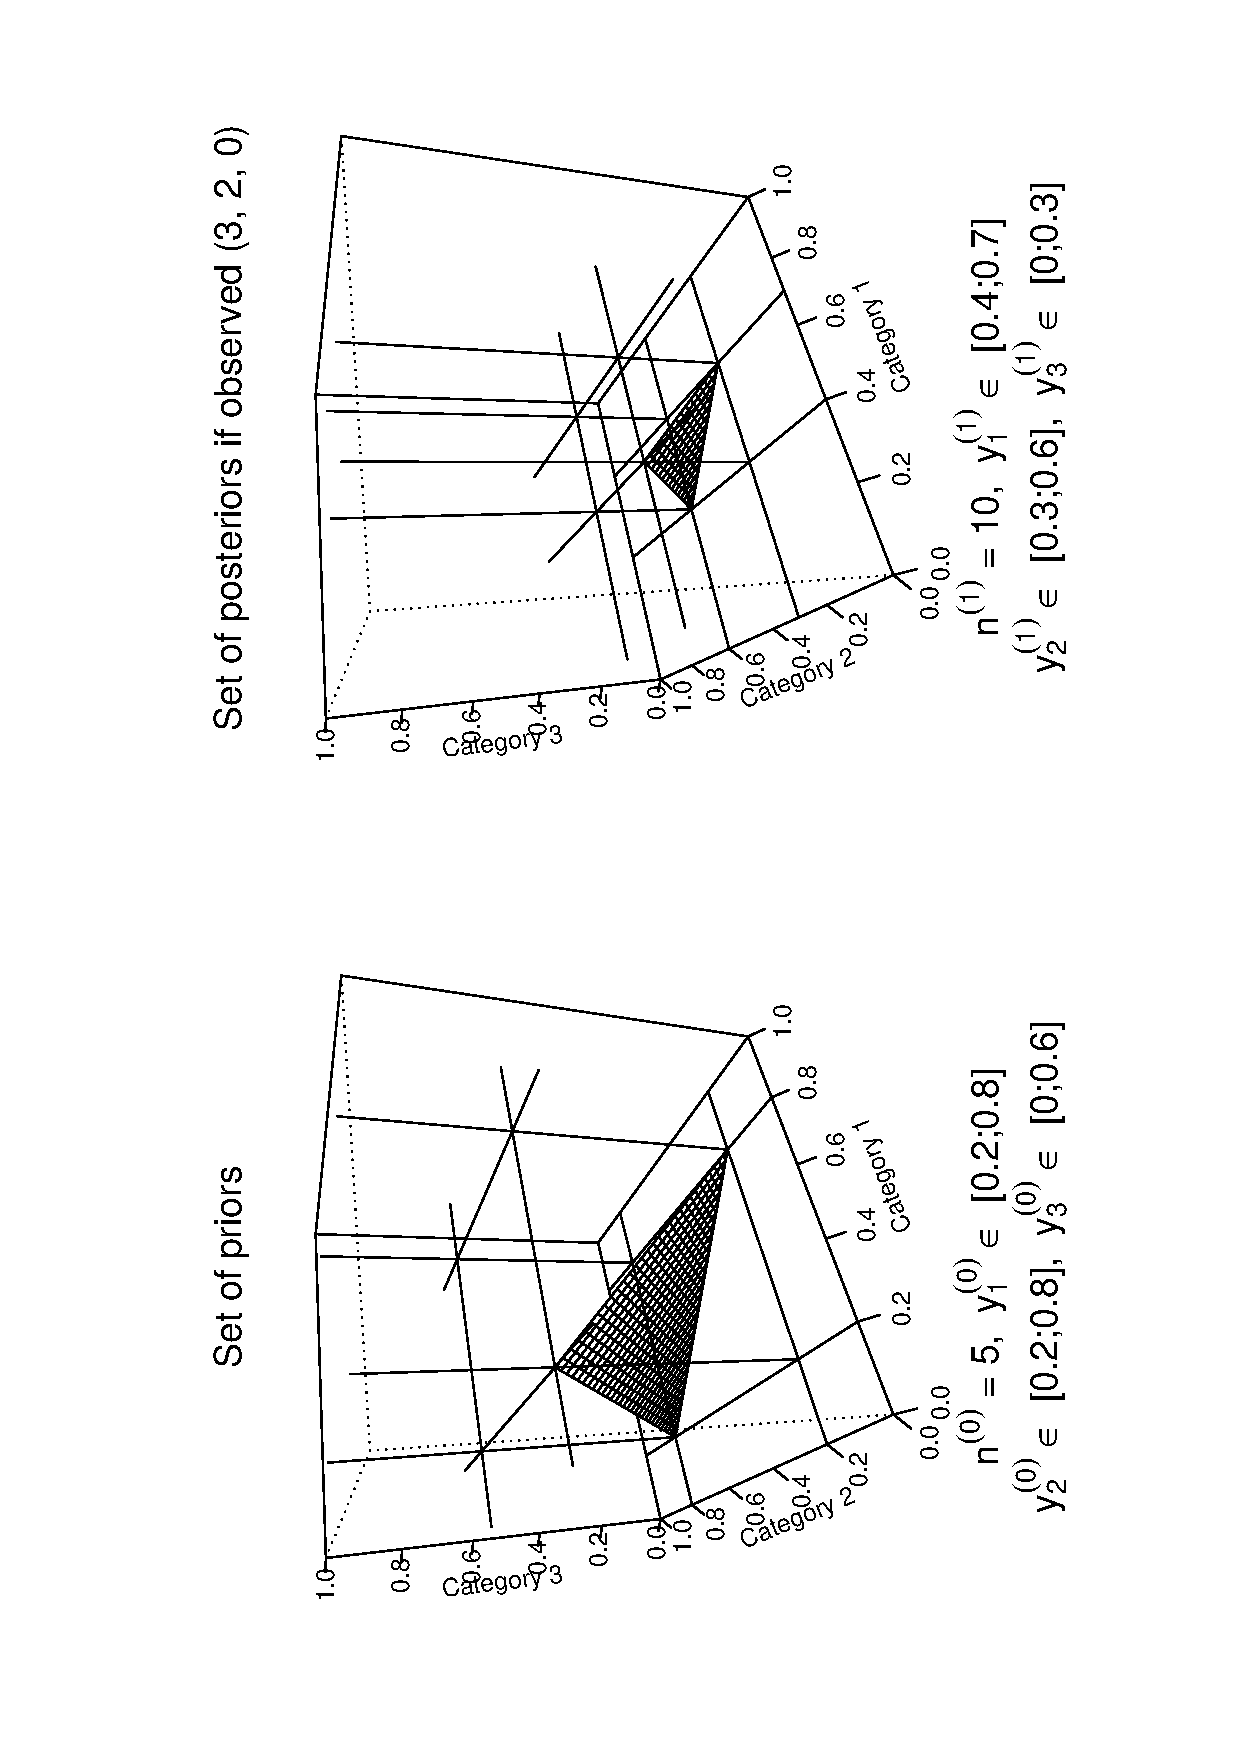
\includegraphics[trim =  20mm 25mm 150mm 20mm, clip, width=0.33\textwidth]{fig/jstp-paper_idm_nfest_01-080331}%
\hspace*{-1.2ex}%
&%
\hspace*{-1.2ex}%
%\includegraphics[height=0.33\textwidth,angle=-90,bb = 100 470 520 790]{fig/jstp-paper_idm_nfest_01-080331.ps}%
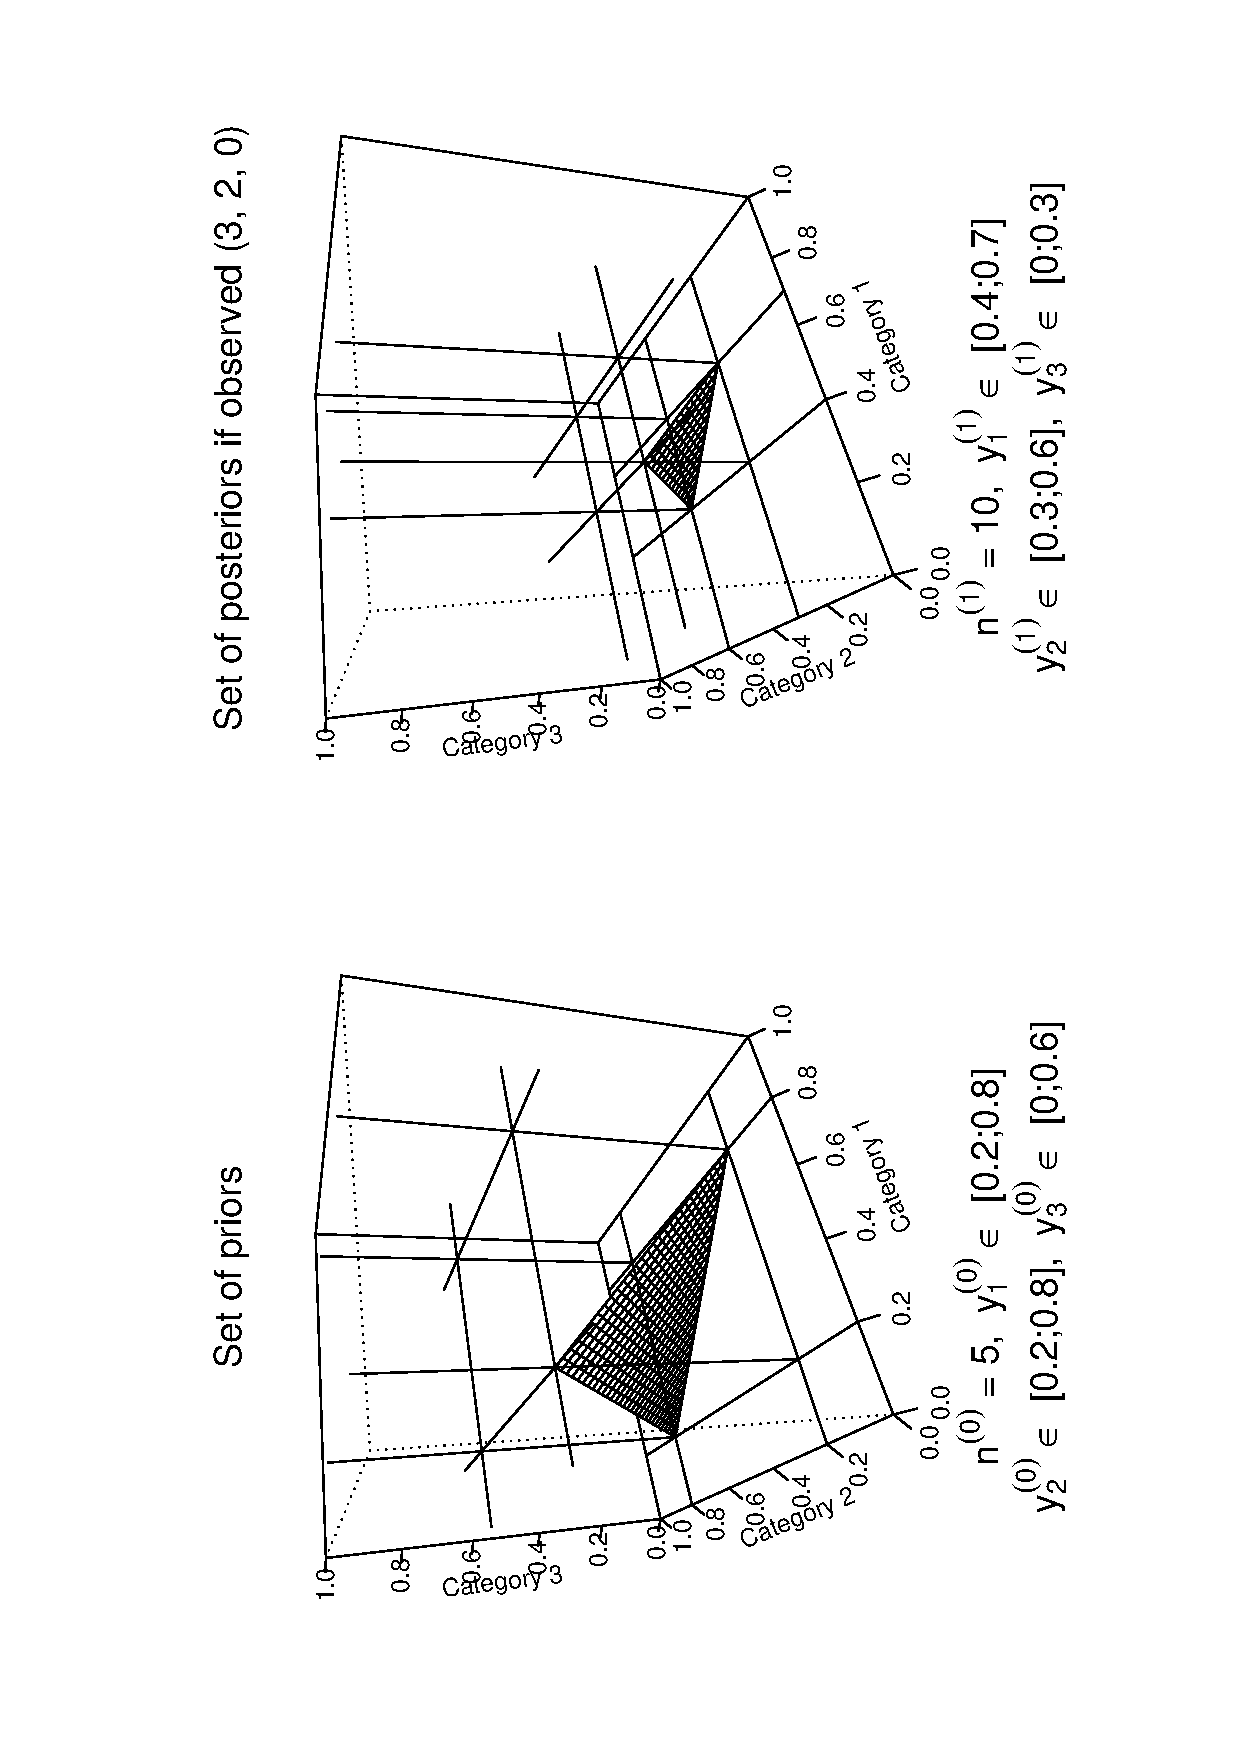
\includegraphics[trim = 150mm 25mm  20mm 20mm, clip, width=0.33\textwidth]{fig/jstp-paper_idm_nfest_01-080331}%
\hspace*{-1.2ex}%
&%
\hspace*{-1.2ex}%
%\includegraphics[height=0.33\textwidth,angle=-90,bb = 100 470 520 790]{fig/jstp-paper_idm_nfest_02-080331.ps}%
\includegraphics[trim = 150mm 25mm  20mm 20mm, clip, width=0.33\textwidth]{fig/jstp-paper_idm_nfest_02-080331}%
\hspace*{-1.2ex}%
\end{tabular}%
\caption{Prior (left) and posterior (center, right) credal sets for samples from
$\mult(\btheta)$ in accordance with (center) and, as studied in
Section~\ref{section:fixednschlecht}, contrary to (right) prior
beliefs. Note that both posterior sets have the same shape and size and differ
only in location, in contrast to the ones depicted in Figure~\ref{fig:idm-nvar-nopdc}.}
\label{fig:idm-nfest-nopdc}
\end{figure}


\begin{remark} \label{remark:i-v}
%The following list contains important properties of
%inference in \emph{\ymodel s}, \thc{where the first three items} in
%essence \thcc{generalize results} that have been discussed in
%the literature for the IDM, where, as already said above, $n\uz$
%usually is denoted by $s$.\vspace*{-1.5ex}
Inference in \emph{\ymodel s} has the following important properties,
where the first three items in essence generalize results that have
been discussed in the literature for the IDM, where, as already said
above, $\nz$ usually is denoted by $s$.%
\footnote{See the discussion in Section~\ref{sec:gbicp-properties-criteria}.***}
\begin{enumerate}[i)]
\item The larger $\nz$ relative to $n$, the more weight is placed on
the prior knowledge expressed by $\YZ$, resulting in wider
posterior expectation intervals and larger ${\rm MPI}\un$.
\item For growing sample sizes $n$, the set $\YN$ will
converge towards a one-element set, as the weight of the `imprecise'
$\YZ$ decreases with respect to the `precise' sample
$\ttau(\x)$, ultimately resulting in an (almost)
precise posterior with ${\rm MPI}\un=0$ just as in
classical methods.
\item In particular, for $\nz = n$, the width of the posterior
expectation interval is half the width of the prior interval,
i.e., ${\rm MPI}\un = \frac{1}{2}{\rm MPI}\uz$.
This property is easily derived from \eqref{equ:ymodel-ydiff}
below, and provides another vivid interpretation of $\nz$.
\item Ceteris paribus, a smaller choice of $\YZ$ will result
in a smaller $\YN$, leading to more precise inference
statements as opposed to the choice of a larger $\YZ$.%
\footnote{This item has not been widely considered in
the context of the IDM, which typically is used to
describe inference from a state of prior ignorance.}
\item For the main posterior parameter imprecision, we obtain:
\begin{align}\label{equ:ymodel-ydiff}
{\rm MPI}\un &= \frac{\nz \left( \yzu - \yzl \right)}{\nz + n}.
\end{align}
\end{enumerate}
\end{remark}%\vspace*{-1.5ex}
While items i) -- iv) demonstrate the intuitively appealing
behavior of \ymodel s, we are seriously concerned with %respect to
the fact that ${\rm MPI}\un$ is independent of $\ttau(\x)$,
and, as studied in more detail in the next subsection, therefore
insensitive to prior-data conflict.


\subsubsection{\ymodel s and Prior-Data Conflict}
\label{section:fixednschlecht}
In the linear setting of \ymodel s, the generic concept of prior-data conflict
can be formalized by considering the distance of the observed quantity $\ttau(\x)$ to
its nearest prior guess $\yz \in \YZ$:
%
\begin{definition}[(Degree of) Prior-Data Conflict]\label{080307-defin-pdc}
For \ymodel s, the degree of prior-data conflict can be defined %naturally
as
\begin{equation}\label{se-071217}
%\Delta \left(\frac{\tau^n(x)}{n};\, \ul{y}\uz,\,\ol{y}\uz\right)
%= \inf \left\{ \left| \frac{\tau^n(x)}{n} - y\uz \right|: \ul{y}\uz \leq y\uz \leq \ol{y}\uz \right\}\,.
\Delta \left(\ttau(\x);\, \yzl,\,\yzu\right)
:= \inf \left\{ \left| \ttau(\x) - \yz \right|: \yzl \le \yz \le \yzu \right\}\,.
\end{equation}
Consequently, if
$\Delta \left(\ttau(\x);\, \yzl,\,\yzu\right) > 0$,
we have an instance of prior-data conflict.%
\footnote{Instead of $\Delta(\;\;) > 0$, one could also consider some
threshold $\Delta(\;\;) > \varepsilon > 0$ as a criterion for prior-data conflict, making
Definition~\ref{080307-defin-pdc} also reasonable for \model s.
However, with respect to Remark~\ref{remark8} below, we prefer $\varepsilon = 0$.}
\end{definition}
This Definition can be illustrated by, e.g., Example~\ref{ex:ymodel-nv}, where $\ttau(\x) = \bar{x}$
is the sample mean. A sample mean outside $\YZ$, the a priori assumed interval
of means for the normal distribution on $\mu$, is an instance of prior-data conflict.
If a sample mean of $8$ was observed in the numerical example discussed above, where
$[\yzl ; \yzu] =[3;4]$ had been assumed, we would obtain $\Delta(\;) = 4$,
formalizing our intuition that prior-data conflict is at hand.

As we argued in Sections~\ref{sec:motivation:pdc} and **intro-here**,
imprecise probability models that allow to take prior information into account
should lead to more imprecision if prior-data
conflict is present than in situations where it is not.
%
It is easy to see that \ymodel s do not fulfill this property
because the main parameter posterior imprecision in
\eqref{equ:ymodel-ydiff} does not depend on the sample statistic
$\ttau(\x)$. Thus, for any sample of size $n$, an \ymodel\ leads
to the same main parameter posterior precision gain
whether the sample supports the prior assumptions modelled in
$\YZ$ or it confronts them. As a consequence of the
Bayesian paradigm that all inference is only allowed to depend on
the posterior, this holds also for all derived quantities
like HD intervals. To make this concrete,
let us continue Examples~\ref{ex:ymodel-nv} and \ref{ex:ymodel-idm}.

\begin{figure}
%\includegraphics[height=\textwidth,angle=-90,bb = 165 60 440 765]{fig/jstp-paper_nv_nfest_02-080331.ps}%
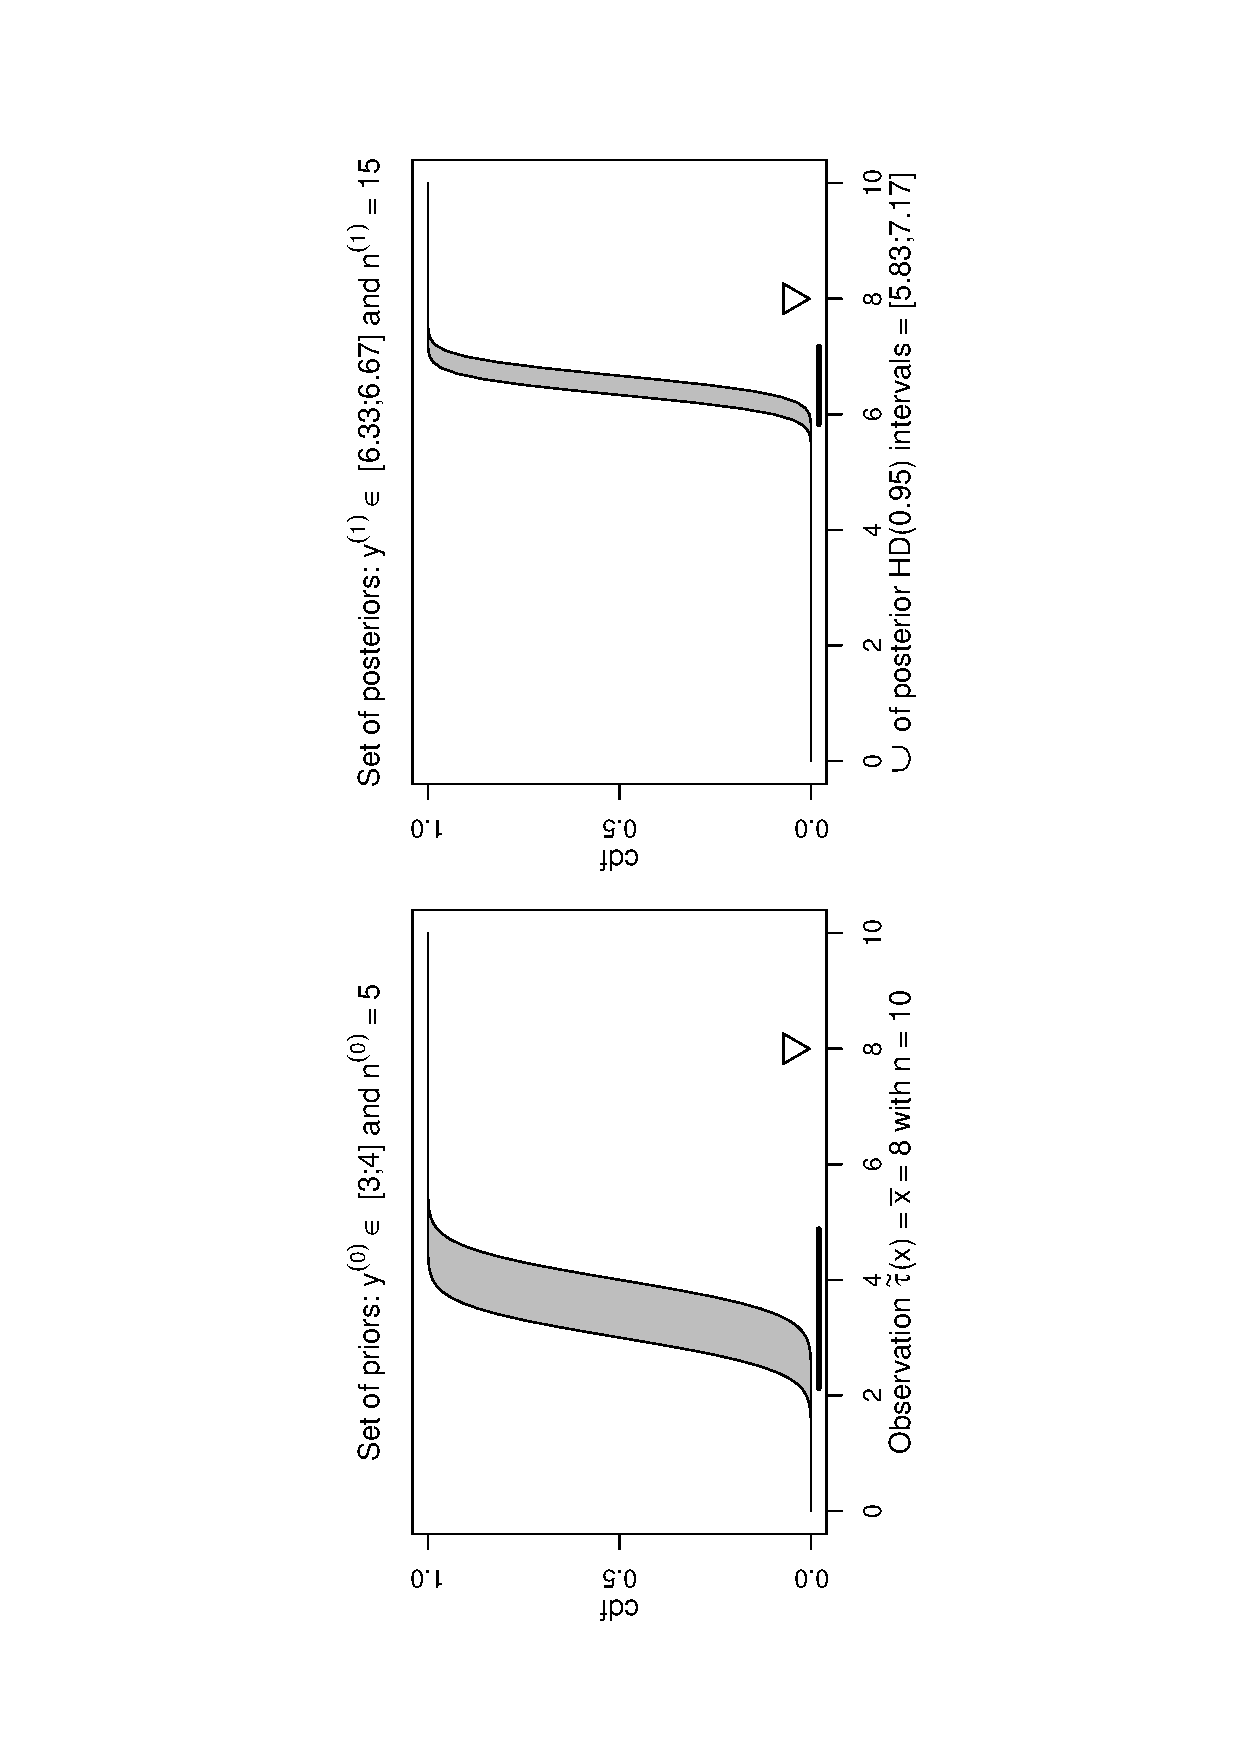
\includegraphics[trim = 20mm 50mm 20mm 50mm, clip, width=\textwidth]{fig/jstp-paper_nv_nfest_02-080331}%
\caption{In \ymodel s, an observation contrary to prior beliefs leads to
the same amount of imprecision as an observation in accordance with prior
beliefs (see Figure~\ref{fig:nv-nfest-nopdc}).  Generalized \ymodel s overcome this
deficiency, as visualized in Figure~\ref{fig:nv-nvar-vertfu}.}
\label{fig:nv-nfest-pdc}
\end{figure}

\begin{example}[Normal-Normal Model, continued]
\label{ex:jstp-5}
%\noindent\textbf{Example 1a (continued).}
Assume, in the situation considered in Section~\ref{070514-secImpPriorLUCK-QdC},
that the sample had led to $\ttau(\x) = 8$,
suggesting the mean $\mu$ to be nearer to $8$ than to the range $[3;4]$ assumed
for it before having seen the sample.
Then $\YN = [\frac{95}{15} ; \frac{100}{15}] \approx [6.33 ; 6.67]$ and again
$\nn = 15$. The posterior range of expected values for $\mu$ has now moved
towards the value suggested by the sample, but we have the same
posterior main parameter imprecision $\frac{1}{3}$ as in the
case with $\ttau(\x) = 4$, which was not conflicting with the prior
assumptions. Intuitively, this fact gets maybe more perplexing when
considering the union of posterior HD intervals: For $\ttau(\x) = 4$,
it is $[3.161;\, 4.506]$, covering a length of $1.345$; for
$\ttau(\x) = 8$, it is $[5.827;\,7.172]$, covering the very same
length, and therefore -- although being completely surprised by the
outcome of the sample -- we would not be more cautious.
These disturbing results are illustrated in Figure~\ref{fig:nv-nfest-pdc}.
\end{example}

\begin{example}[Dirichlet-Multinomial Model, continued]
\label{ex:jstp-6}
%\noindent\textbf{Example 1b (continued).}
Here, the same phenomenon occurs:
Having observed categories 1 to 3 now $0$, $1$, and $4$
times, respectively, $\YN$ covers the same area, despite of the clear conflict of these
observations with the prior knowledge expressed in $\YZ$,
and has only moved in location, as can be seen
in the right graph of Figure~\ref{fig:idm-nfest-nopdc}.
\end{example}


\subsection{Improved imprecise priors for inference in \model s}
\label{sec:4-gw-071216}

There do exist some imprecise probability models that react on
prior-data conflict in reasonable ways. The approaches by
\textcite{1991:pericchi} and \textcite{1994:coolen}
are restricted to specific one-parameter situations with a different type
of models for the prior. \textcite{2005:whitcomb}, on
the other hand, by partially relying on models from the exponential
family, considers closely related classes of underlying
distributions without using their specific structure. The important
hint for properly handling prior-data conflict in
\model s is again obtained from \textcite{1991:walley}.
In \S 5.4, he discusses prior-data conflict in the imprecise
Beta-Binomial model,%
\footnote{See Section~\ref{sec:beta-binom}.}
which is a special case of the Imprecise
Dirichlet Model recalled in Example~\ref{ex:ymodel-idm}. His successful idea is to
vary the hyperparameter $s$ in addition. Additionally, he also
briefly mentions the normal case underlying Example~\ref{ex:ymodel-nv}
\parencite[\S 1.1.5 (k)]{1991:walley}, where he suggests to use an
imprecise prior with an imprecise variance. In the light of the
general framework of \model s, both exemplary solutions
can be subsumed under the idea to use an imprecise prior strength,
thus weighting prior and sample information in
\eqref{equ:shifttrans} in a more flexible way, i.e.\ to vary
additionally the prior strength parameter $\nz$ in some set $\NZ$.
Indeed this way to proceed will turn out to be successful.
We start by describing the powerful generalization we want to
propose in more detail and then discuss some of its basic
properties.
%
%
%
%
\begin{definition}[\nymodel s]\label{071221-def}%
%Consider the Imprecise Probability model as described in \mycite{QdC} %Quaeghebeur and de Cooman (2005),
%or, more generally, a \textsc{LUCK}-model,
Consider the situation of Definitions~\ref{070503-defin1}
and \ref{071219-def2}, and a set of LUCK-models
$\big(p(\vartheta),p(\vartheta\mid\x)\big)$ that is produced by
$\yz$ varying in some set $\YZ \subset \Y$
and, in addition, $\nz$ varying in a set $\NZ \subset \posreals$.
Let furthermore again the credal sets ${\cal M}$ and ${\cal M}_{|\x}$ consist
of all convex mixtures obtained from this variation of $p(\vartheta)$ and
$p(\vartheta\mid\x)$. Then $\big({\cal M}, {\cal M}_{|\x}\big)$ is
called the corresponding \emph{\nymodel } based on $\YZ$ and $\NZ$.
\end{definition}

\begin{remark}
Again, by construction, when ${\cal M}$ is used as an
imprecise prior,  ${\cal M}_{|\x}$ is the corresponding posterior. It is obtained
as the set of all convex mixtures of
distributions defined by the parameter set
\begin{equation*}
%\left\{\!\! \left. \left(\!n\uo,\, y\uo\! \right) \; \right| \; n\uo = n\uz + n,\, y\uo = \frac{n\uz y\uz + \tau(x)}{n\uz+n},\,
%n\uz \in {\cal N}\uz,\, y\uz \in {\cal Y}\uz \!\right\}
\left\{ \left. \left(\nn,\yn\right) \; \right| \, \nn = \nz + n,\, \yn = \frac{\nz\yz + \tau(\x)}{\nz + n},\,
\nz \in \NZ,\, \yz \in \YZ \right\}\,.
\end{equation*}
Note that the set of posterior parameters is not a cartesian product, i.e., rectangular. However,
extreme values for the main posterior parameter $\yn$ are still easy to derive:%
\footnote{As $\frac{d}{d \yz}\, \yn = \frac{\nz}{\nz + n} \ge 0 \;
\forall\, n,\, \nz,\,\tau(\x)$, it holds that $\yn$ is growing in
$\yz$ regardless of the value of $\nz$, and thus, for obtaining
$\ynu$, we must insert $\yzu$, and for obtaining
$\ynl$, we must insert $\yzl$ in \eqref{070305-4}, just as
in \ymodel s, where $\nz$ is fixed. Then, with
$\frac{d}{d \nz}\, \yn  = \frac{\yz n - \tau(\x)}{(\nz + n)^2}$, we see that $\yn$
is growing in $\nz$ if $\yz > \ttau(\x)$ and decreasing in
$\nz$ if $\yz < \ttau(\x)$, leading to
Equations~\eqref{equ:uly1-071206} and \eqref{equ:oly1-071206}.}

\begin{align}
\ynl &= \label{equ:uly1-071206}
\begin{cases}
\frac{\nzu \yzl + \,\tau(\x)}{\nzu + n} & \text{if}\quad \ttau(\x) \ge \yzl\\[1.5ex]
\frac{\nzl \yzl + \,\tau(\x)}{\nzl + n} & \text{if}\quad \ttau(\x) <   \yzl
\quad\Longleftrightarrow\quad \text{prior-data conflict}
\end{cases} \\[1ex]
\ynu &= \label{equ:oly1-071206}
\begin{cases}
\frac{\nzu \yzu + \,\tau(\x)}{\nzu + n} & \text{if}\quad \ttau(\x) \le \yzu\\[1.5ex]
\frac{\nzl \yzu + \,\tau(\x)}{\nzl + n} & \text{if}\quad \ttau(\x) >   \yzu
\quad\Longleftrightarrow\quad \text{prior-data conflict}.
\end{cases}
\end{align}
\end{remark}

For minimizing and maximizing $\yn$, the value $\nzl$ is
used only in the situation of prior-data conflict, that is, if
$\ttau(\x) \notin \YZ$.
When no prior-data conflict occurs, the extreme values are attained for $\nzu$.
%
Therefore, the fixed value of $\nz$ in \ymodel s in the spirit of \textcite{2005:quaeghebeurcooman} can be
seen as the upper border of an implicit set $\NZ$, and
considering only a fixed $\nz$ means that prior-data conflict is neglected.

On the other hand, if observations are such that
$\ttau(\x) \in \left[\yzl;\,\yzu\right]$, then
no prior-data conflict is present, and inference in \nymodel s
leads to very similar results as inference in \ymodel s.%
\footnote{From \eqref{equ:uly1-071206} and \eqref{equ:oly1-071206}
it gets clear why varying $\nz$ in addition does change the
update step in the desired way. When $\ttau(\x) < \yzl$,
then $\nzu$ is still used to calculate $\ynu$, but
$\nzl$ to calculate $\ynl$. The use of $\nzl$ instead
of $\nzu$ results in a lower value for $\yzl$, as then
more weight is given to $\ttau(\x)$ with respect to
$\yzl$. (Equation~\eqref{equ:shifttrans} makes this most
visible.) The same type of reasoning applies for the case
$\ttau(\x) > \yzu$, where $\nzu$ is still used to
calculate $\ynl$, but $\nzl$ to calculate $\ynu$.}

\begin{remark}\label{remark8}
By construction, the attractive properties of inferences by
\ymodel s formulated in i) to iv) of Remark~\ref{remark:i-v}
are still satisfied in our extended model. Now
also in addition prior-data conflict is handled in a
convincing way: Considering the relationship between the main
parameter posterior imprecision defined as in
\emph{\eqref{071214-4}} and the degree of prior-data conflict
as defined in \emph{\eqref{se-071217}},%
\footnote{Remark~\ref{071221-remark} and Definition~\ref{080307-defin-pdc} can directly be applied also to \nymodel s.}
the very same results as derived by \textcite[p.~224]{1991:walley}
for the two-category Dirichlet-Multinomial model hold in general
for any \nymodel: %\vspace*{-1.0ex}

%Using the update rules for varying $n\uz$, we get,
%just as described in Walley (1991, p.~224) for a two-category IDM,
%a posterior range of
%\vspace*{-3.0ex}
\begin{align*}
{\rm MPI}\un &= \frac{\nzu (\yzu - \yzl)}{\nzu + n}
                + \Delta \left(\ttau(\x);\, \yzl,\,\yzu\right)
                  \, \frac{n (\nzu - \nzl)}{(\nzu + n)(\nzl + n)}\,.%
\end{align*}
%\vspace*{-1.0ex}
It is only through $\Delta(\;)$ that ${\rm MPI}\un$ is 
depending on the actual shape of observation $\x$ besides its size
$n$, and increasing it if prior-data conflict occurs. When no
prior-data conflict is present, $\Delta \left(\ttau(\x);\,\yzl,\,\yzu\right) = 0$,
and we have the same amount of posterior imprecision in substantial parameters as in \emph{\ymodel s},
given by \emph{\eqref{equ:ymodel-ydiff}}.
%
Consequently, Walley's \parencite*[\S 5.4, footnote~3]{1991:walley} observation
that the factor to $\Delta(\;)$ gets maximal if $n = \big(\nzl\nzu\big){}^\frac{1}{2}$
remains valid. Then, the main parameter posterior imprecision
is maximal for a given degree of conflict, implicitly telling that
then the weight of the prior and sample must be the same, as more
weight on any of them compared to the other (preferring one source
of information to the other) would lead to a less wide $\YN$.
This fact gives additional orientation for choosing $\NZ$,
by considering the global strength of prior knowledge,
being equivalent to $\ul{\ol{n}}\uz := \big(\nzl\nzu\big){}^\frac{1}{2}$.
\end{remark}

\begin{figure}
%\includegraphics[height=\textwidth,angle=-90,bb = 90 60 515 770]{fig/jstp-paper_nv_nvar_vertfu01_081128.ps}%
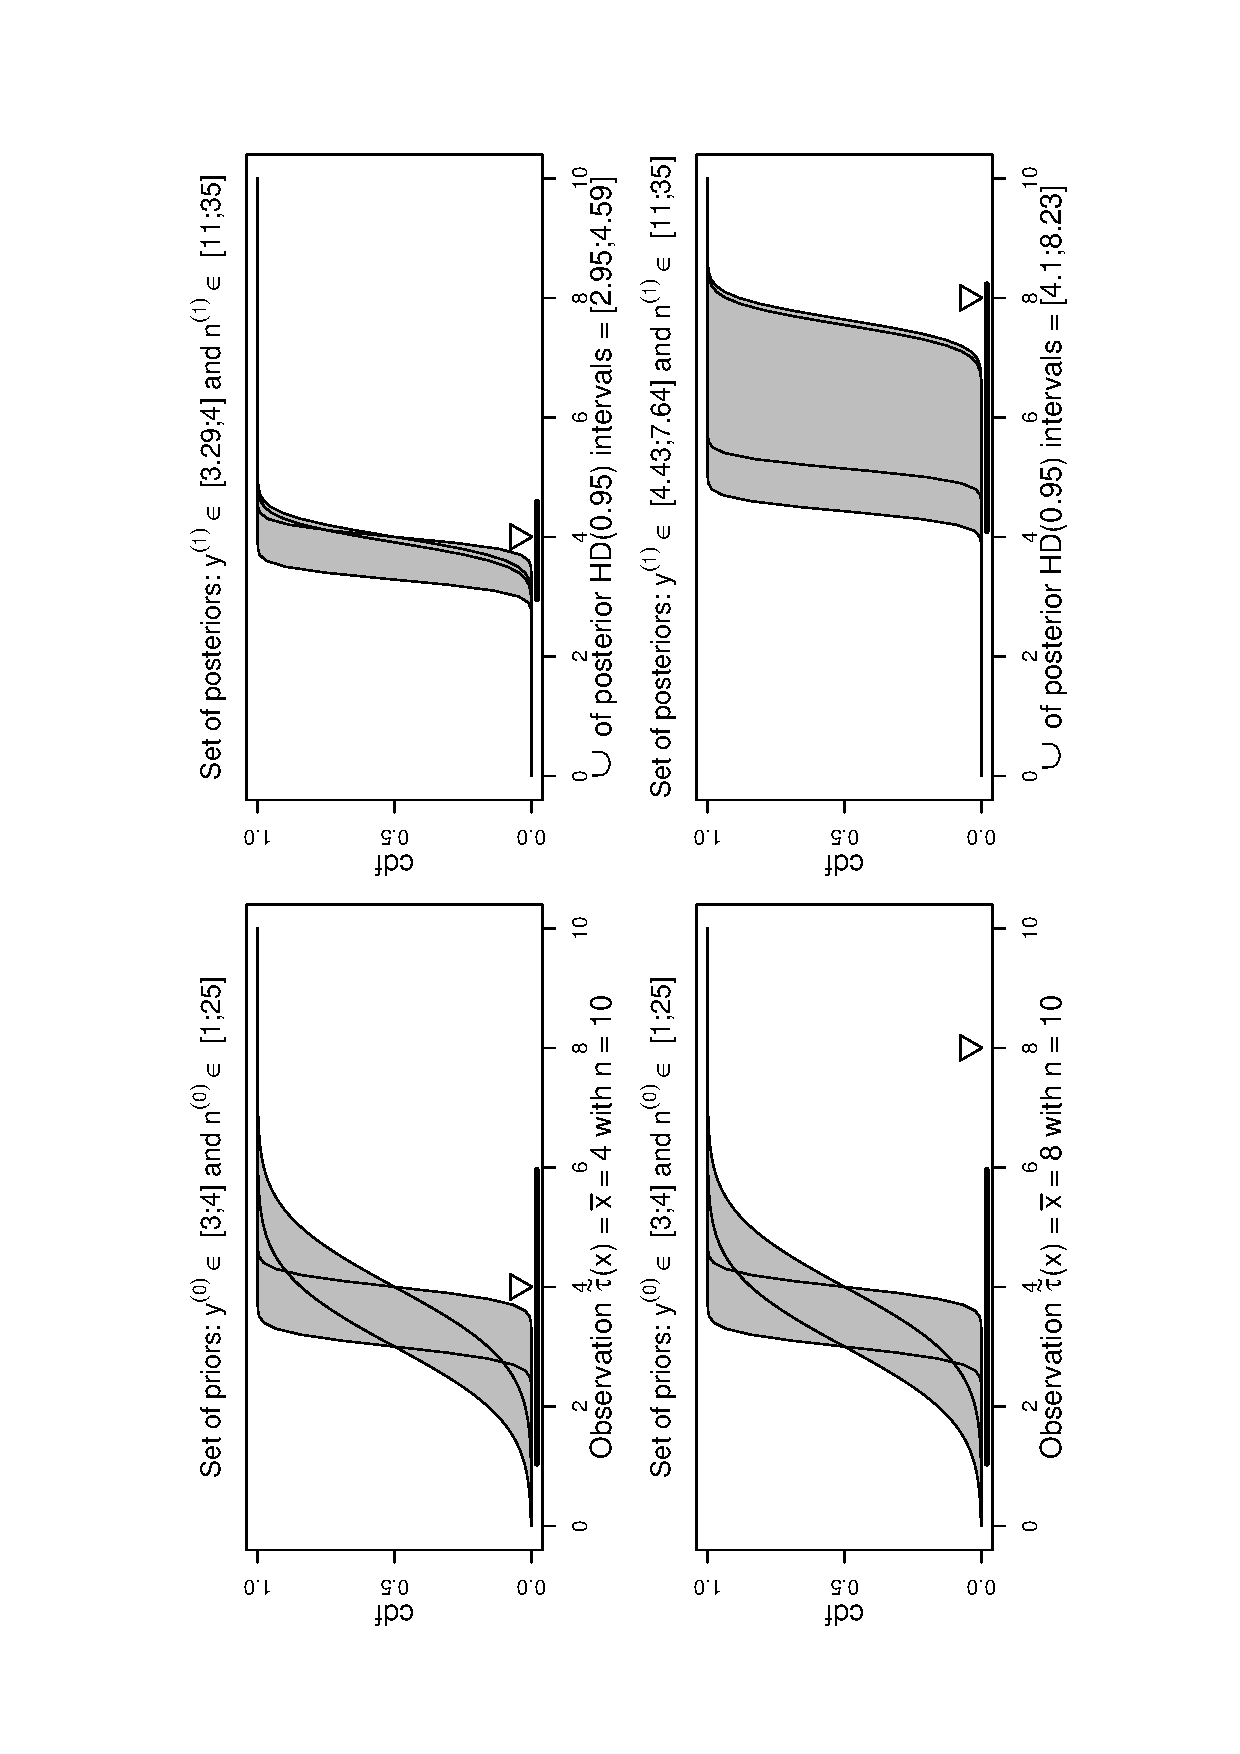
\includegraphics[trim = 20mm 20mm 20mm 25mm, clip, width=\textwidth]{fig/jstp-paper_nv_nvar_vertfu01_081128}%
\caption{Prior (left) and posterior (right) credal sets for samples from
$\norm(\mu,1)$ in accordance with (upper) and contrary to (lower)
prior beliefs. With \nymodel s, the posterior set in the latter case is
significantly larger than in the former, leading to more cautious inference as desired.}
\label{fig:nv-nvar-vertfu}
\end{figure}


\subsection{Illustration of the \nymodel} \label{sec:illu} 

The theoretical considerations in Section~\ref{sec:4-gw-071216} are now
illustrated by means of Examples~\ref{ex:ymodel-nv} -- \ref{ex:jstp-6},
and some simulated data for larger sample sizes.

\begin{example}[Normal-Normal model, continued]
\label{ex:jstp-7}
For the case of the Normal-Normal Model (Examples~\ref{ex:ymodel-nv} and \ref{ex:jstp-5}),
the behavior of an appropriate \nymodel\ is shown for the situations previously
modeled with an \ymodel\ as depicted in
Figures~\ref{fig:nv-nfest-nopdc} and \ref{fig:nv-nfest-pdc}. In
Figure~\ref{fig:nv-nvar-vertfu}, the top row shows the updating in
absence of prior-data conflict, whereas the lower row displays
the update step in presence of prior-data conflict.
Again, the vertices of the credal set, the set of normal
distribution functions, is represented by the shaded area,
and the lines indicate the distributions that are obtained by updating the four
extreme distributions from $\NZ \times \YZ$.

Contrary to the \ymodel, also a range of variances is considered in the
prior, allowing for reasonable posterior inference, as can be seen
in the right hand graphs: when the prior model is consistent with
the observation $\ttau(\x) = \bar{x}$, a similar union of posterior HD
intervals is obtained as for the model displayed in
Figure~\ref{fig:nv-nfest-nopdc}; when instead prior assumptions and
data are conflicting, the posterior credal set reflects our
uncertainty on which to trust, being substantially larger than the
prior credal set. Therefore, the union of posterior HD intervals as
indicated by the thick line in the lower right graph is not only
wider than in the absence of prior-data conflict as seen in the top
right graph, but not much shorter than its prior counterpart which is $[1.040;\, 5.960]$.
In order to give comparable results, $\NZ$ was chosen to give the same global prior strength as the
\ymodel\ for Example~\ref{ex:ymodel-nv} by fixing $\ul{\ol{n}}\uz=5$ and a minimal prior strength
$\nzl = 1$, resulting in $\nzu = 25$.
\end{example}

\begin{figure}
%\fbox{%
\begin{tabular}{ccc}%
\hspace*{-1.2ex}%
%\includegraphics[height=0.33\textwidth,angle=-90,bb = 100 65 520 385]{fig/jstp-paper_idm_nvar_zeile1-080331.ps}%
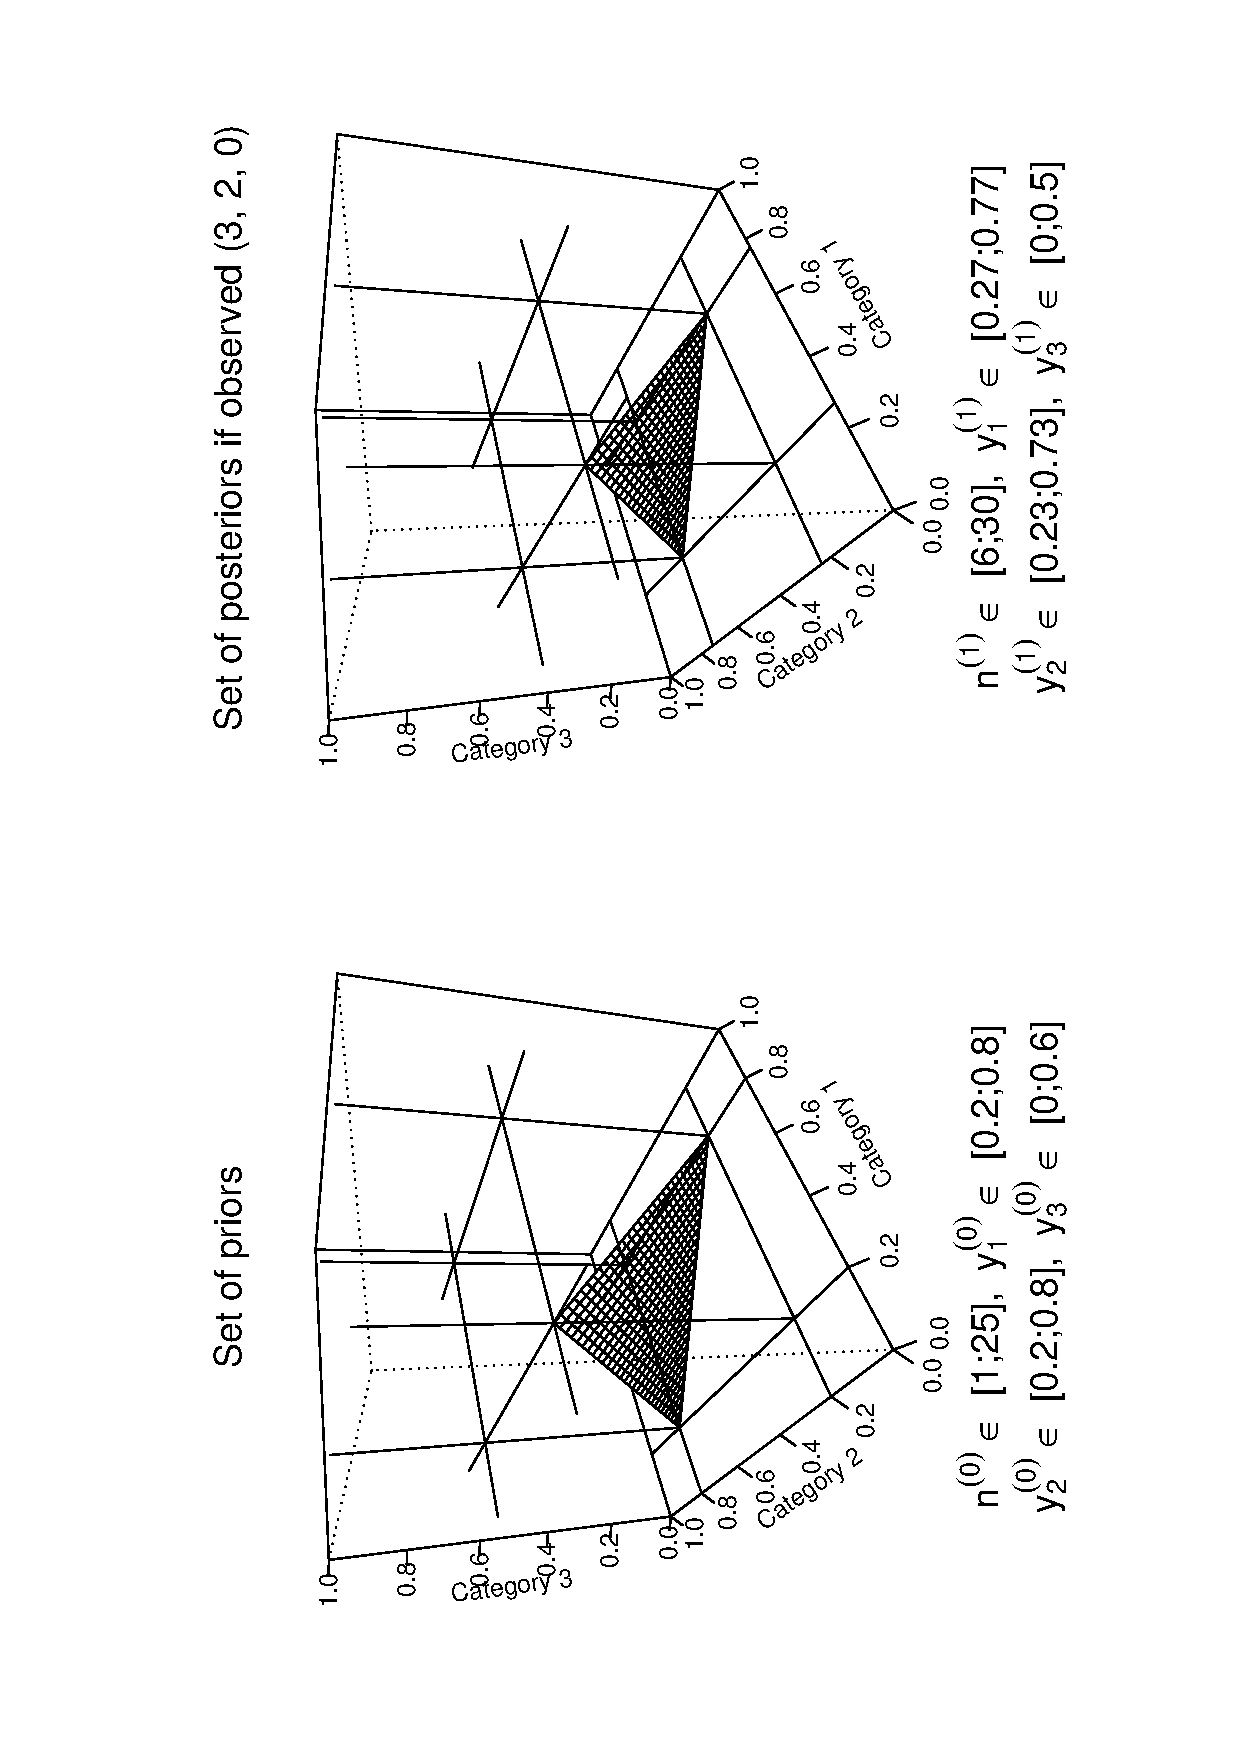
\includegraphics[trim =  20mm 25mm 150mm 20mm, clip, width=0.33\textwidth]{fig/jstp-paper_idm_nvar_zeile1-080331}%
\hspace*{-1.2ex}%
&%
\hspace*{-1.2ex}%
%\includegraphics[height=0.33\textwidth,angle=-90,bb = 100 470 520 790]{fig/jstp-paper_idm_nvar_zeile1-080331.ps}%
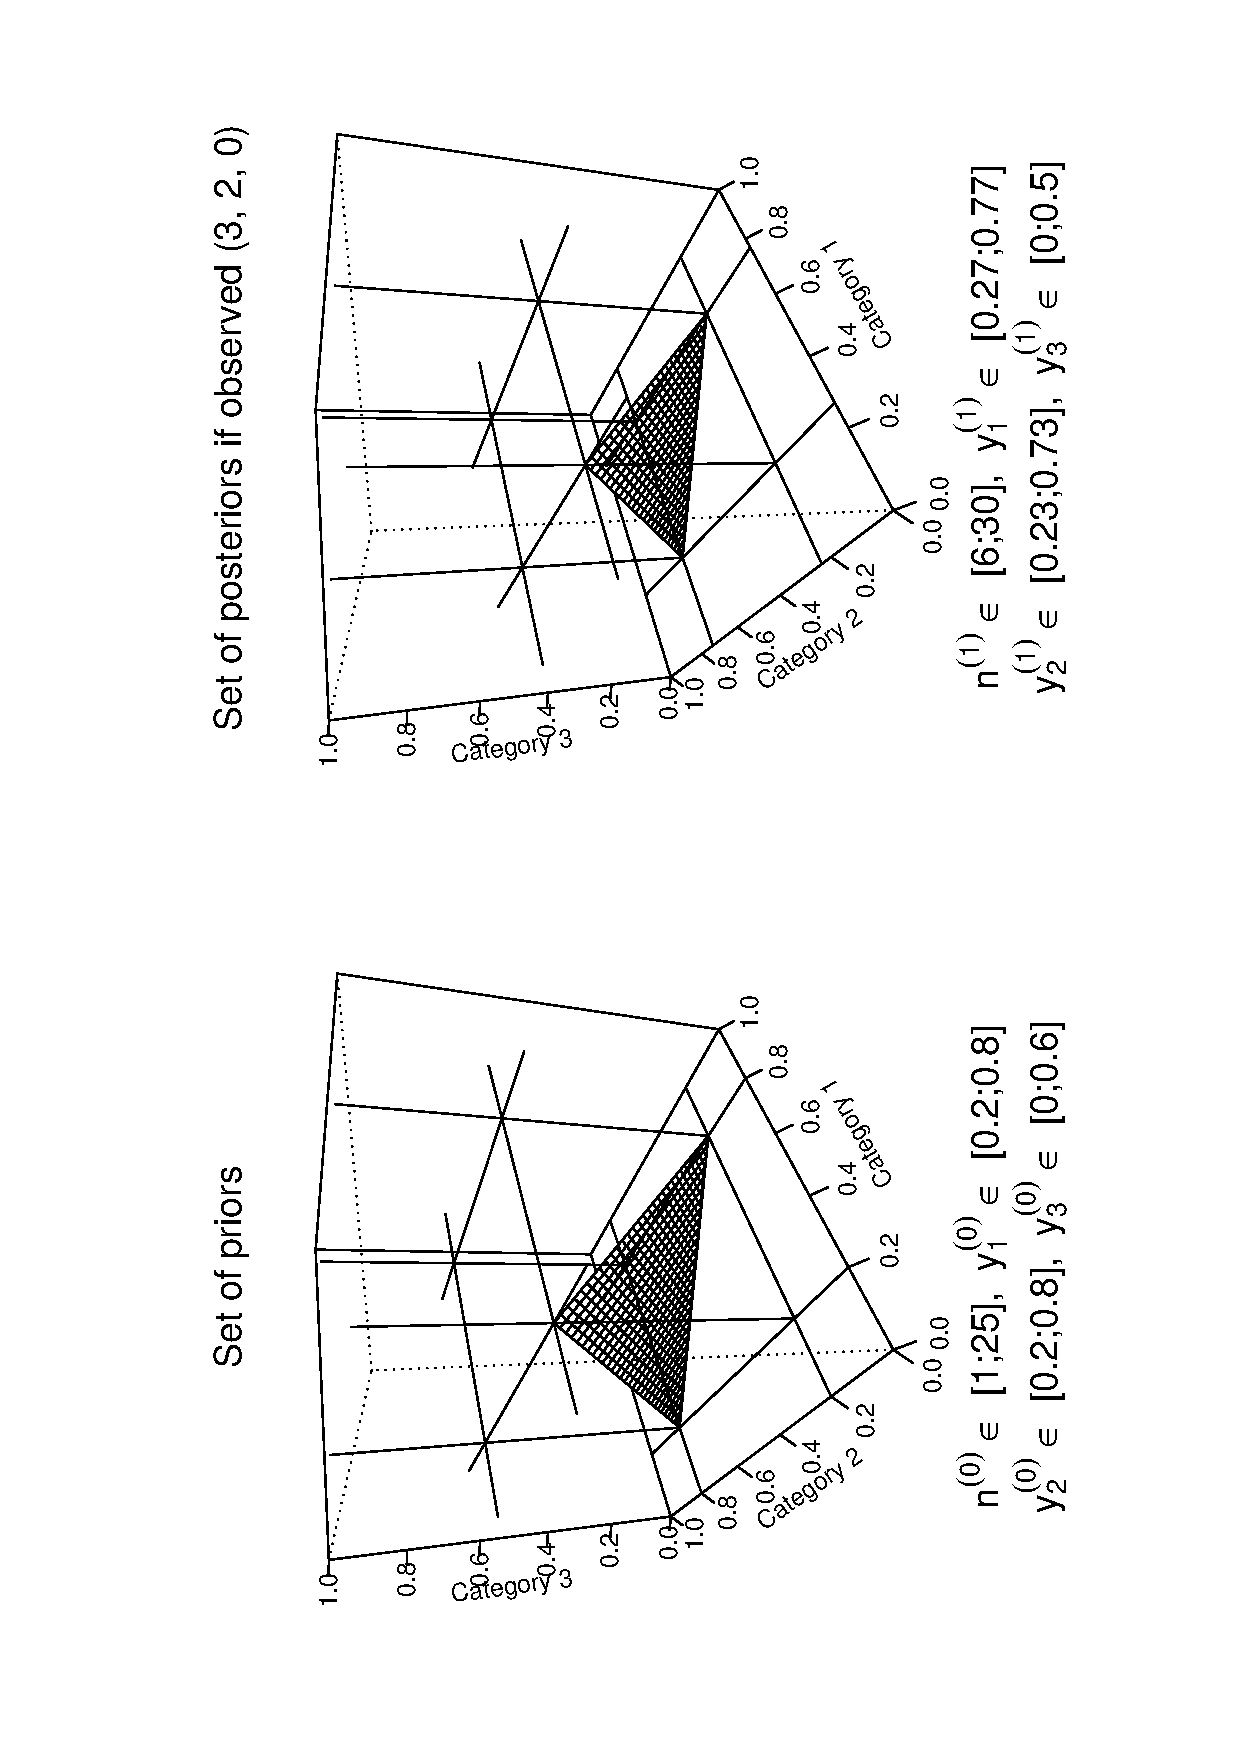
\includegraphics[trim = 150mm 25mm  20mm 20mm, clip, width=0.33\textwidth]{fig/jstp-paper_idm_nvar_zeile1-080331}%
\hspace*{-1.2ex}%
&%
\hspace*{-1.2ex}%
%\includegraphics[height=0.33\textwidth,angle=-90,bb = 100 470 520 790]{fig/jstp-paper_idm_nvar_zeile2-081205.ps}%
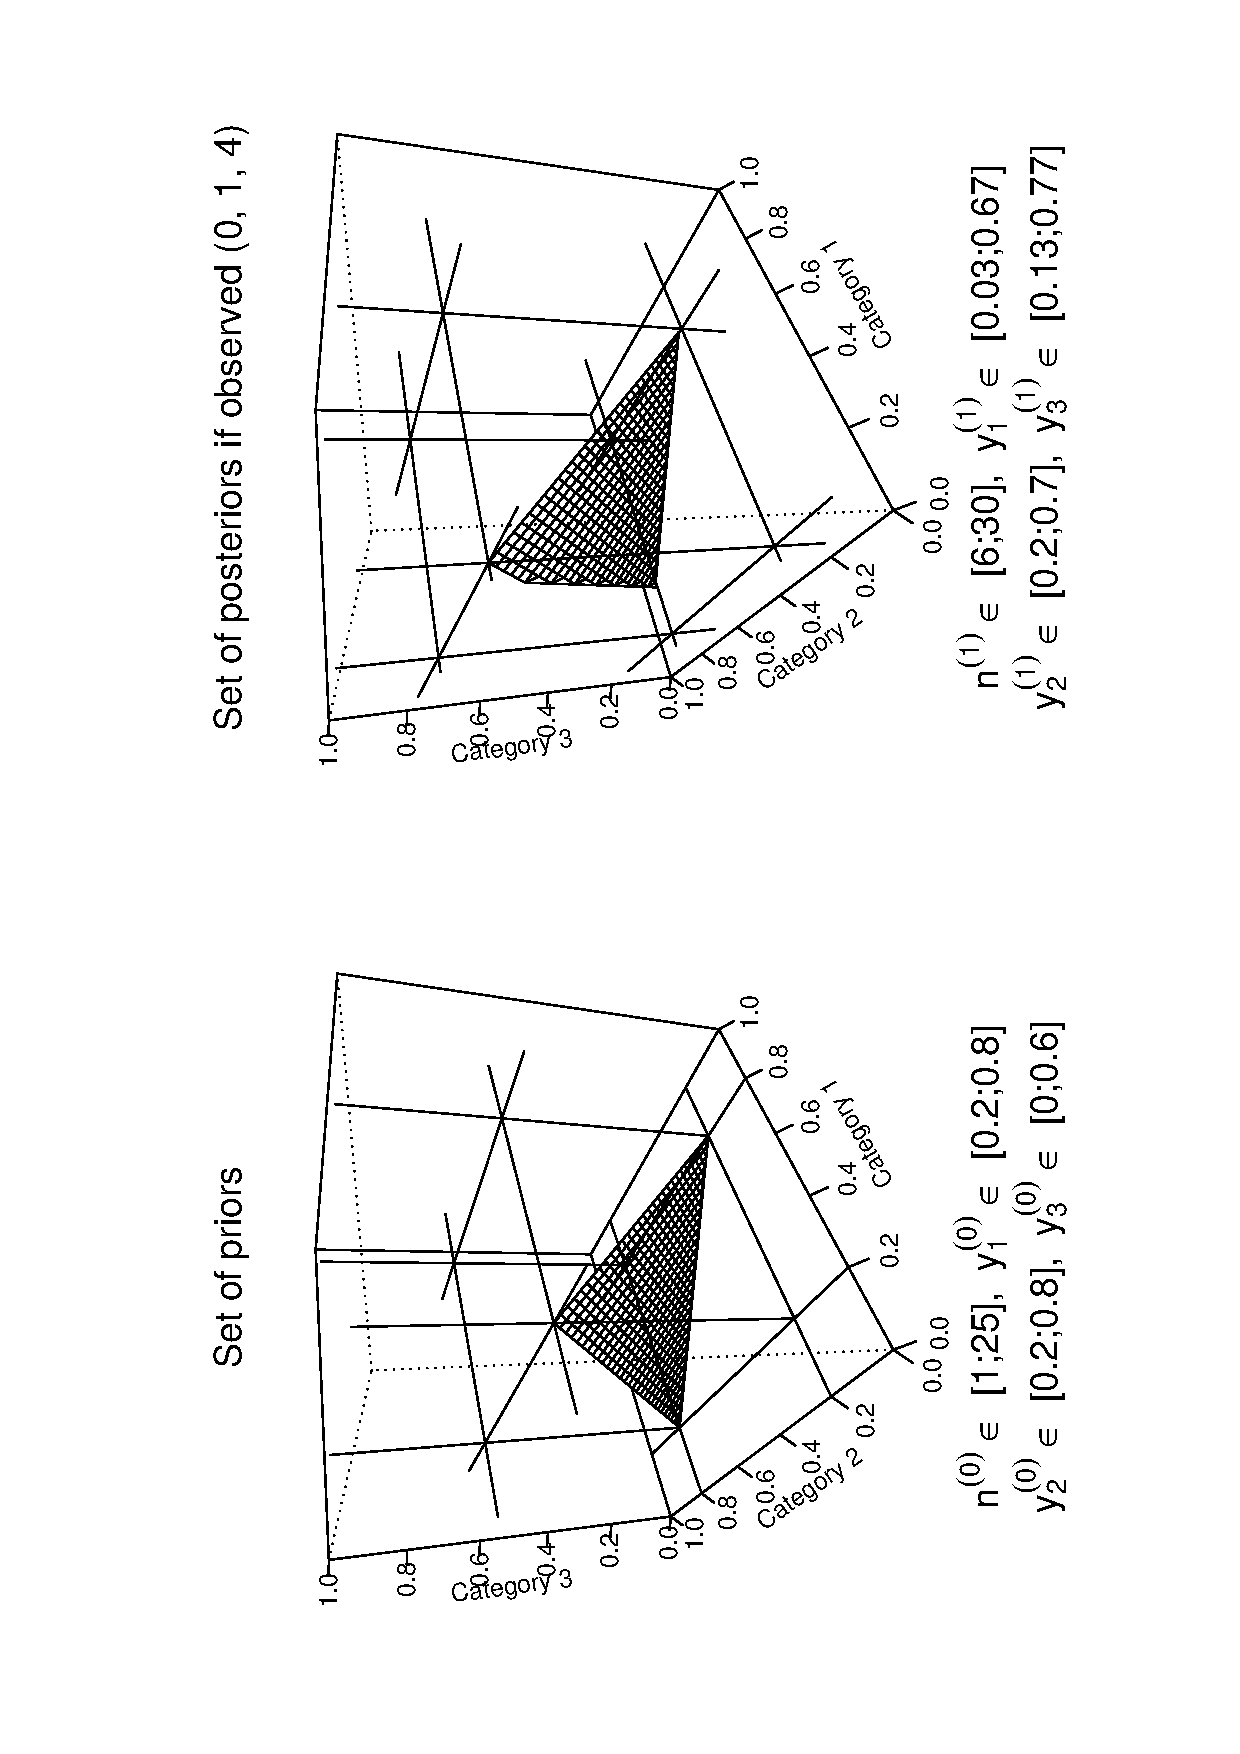
\includegraphics[trim = 150mm 25mm  20mm 20mm, clip, width=0.33\textwidth]{fig/jstp-paper_idm_nvar_zeile2-081205}%
\hspace*{-1.2ex}%
\end{tabular}%
\caption{
Prior (left) and posterior (center, right) credal sets for samples from
$\mult(\btheta)$ in accordance with (center) and contrary to (right)
prior beliefs. As in Figure~\ref{fig:nv-nvar-vertfu}, with \nymodel s
the sets differ in size according to the degree of prior-data conflict
induced by the observations.
}
\label{fig:idm-nvar-nopdc}
\end{figure}


\begin{example}[Dirichlet-Multinomial model, continued]
\label{ex:jstp-8}
For the Dirichlet-Multinomial model (Examples~\ref{ex:ymodel-idm} and \ref{ex:jstp-6}),
the behavior of the \nymodel\ is visualized in Figure~\ref{fig:idm-nvar-nopdc}. Here, the same set
of main parameters as in Figure~\ref{fig:idm-nfest-nopdc} is updated, leading
to plane cutouts (symbolizing posterior parameter sets) that
differ not only in location as before, but also in size (and shape) for the
two cases. For the center graph, prior assumptions on the category
probabilities are in accordance with the observations 3, 2 and 0
for category one, two, and three, respectively, and thus the
posterior plane cutout is a subset of the prior plane. In
contrast, when observations 0, 1, and 4 are made, being in
conflict with the prior assumptions for category one and three,
the resulting posterior parameter intervals for those two
categories do actually get wider, as can be seen in the right
graph, and thus, inference drawn in this case is more cautious.
\end{example}

\begin{figure} %trim = l b r t
%\includegraphics[height=0.99\textwidth,angle=-90,bb = 20 15 575 825]{fig/jstp-paper_nv_nvar_HPD_n-infty_081201.ps}%
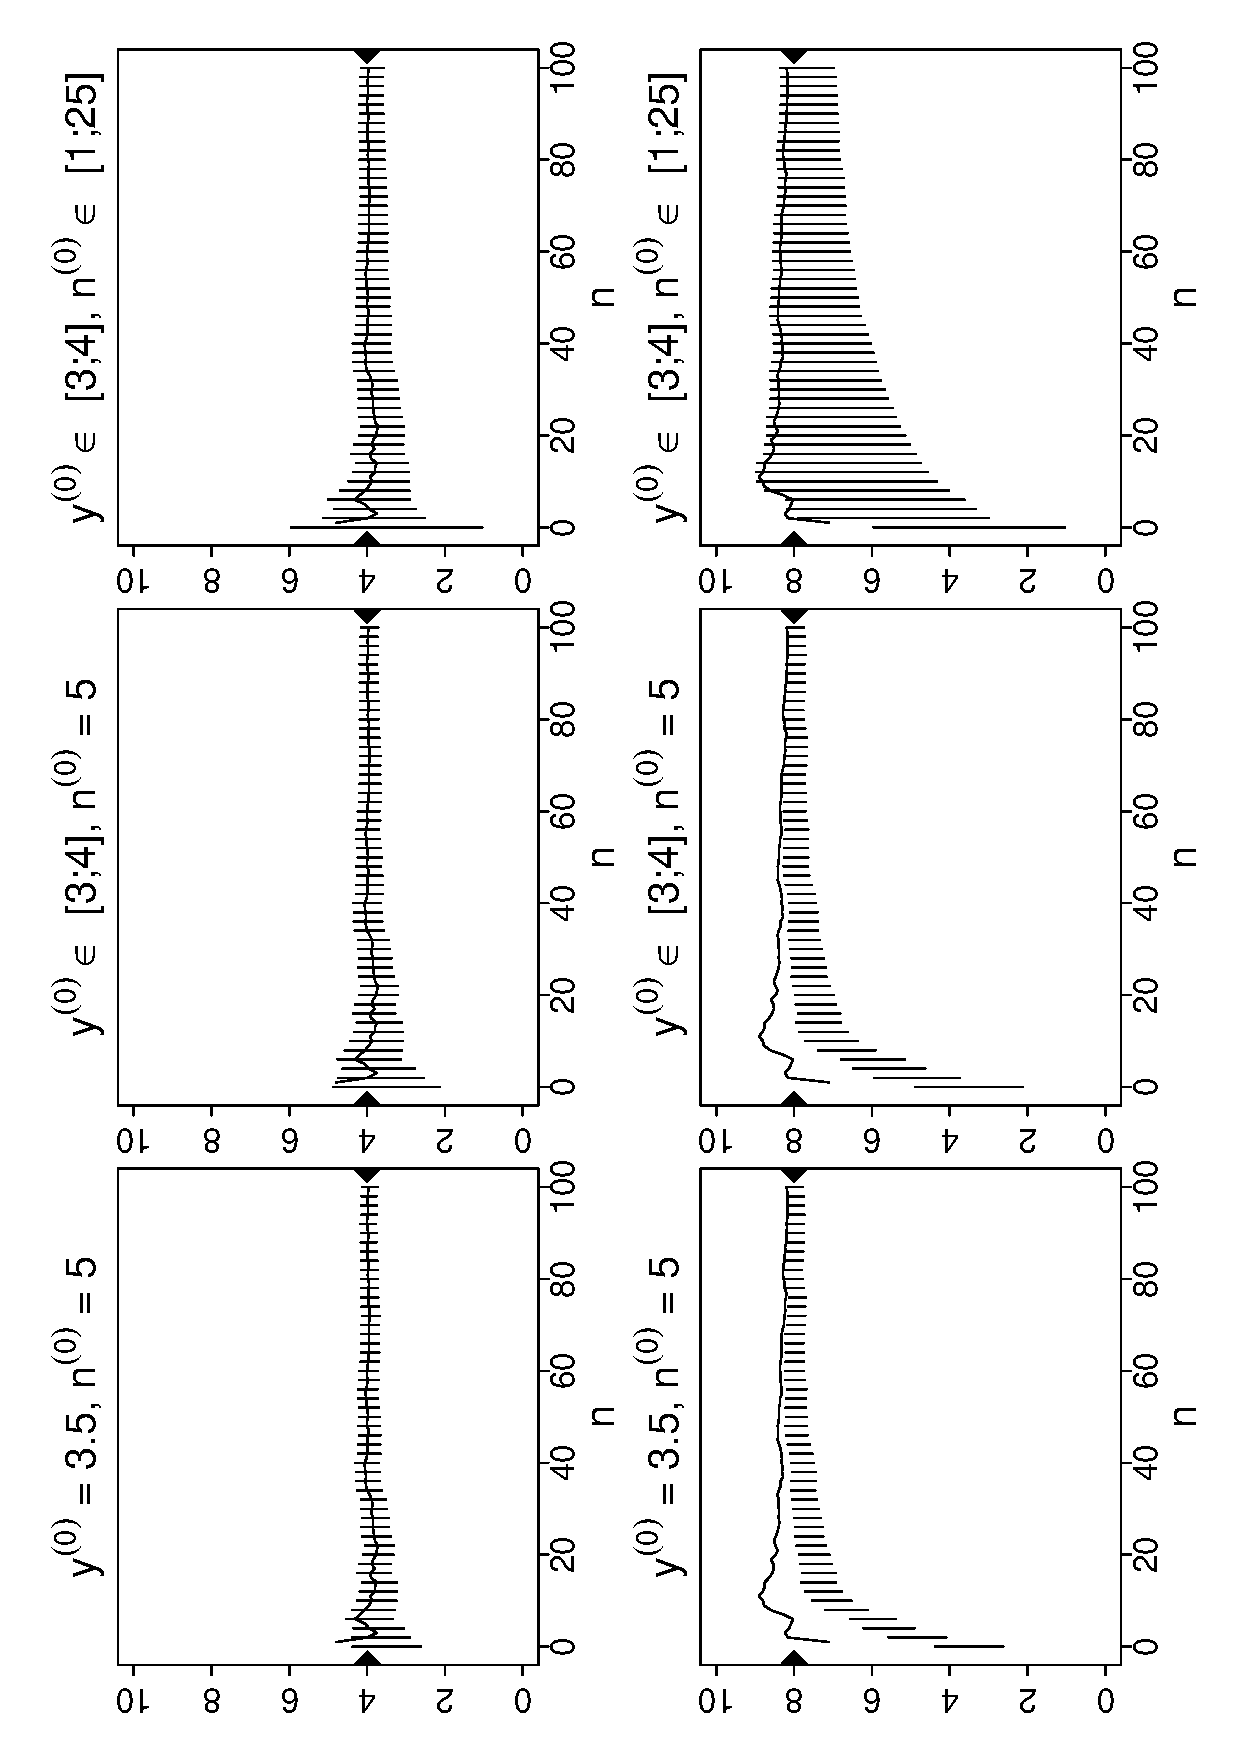
\includegraphics[trim = 5mm 5mm 5mm 5mm, clip, width=\textwidth]{fig/jstp-paper_nv_nvar_HPD_n-infty_081201}%
\caption{(Unions of) 95\%-posterior HD intervals (vertical lines) for
observations in accordance (upper row, drawn from $\mbox{N}(4,1)$)
and in conflict (lower row, drawn from $\mbox{N}(8,1)$) with prior assumptions
based on a single prior (left), an \ymodel\ (center) and a \nymodel\ (right)
in dependence on the sample size $n$. The development of the sample mean is
indicated by the wiggly line. Through the averaging, the HD intervals in the
lower left and center graph are not enlarged but only shifted and thus do not cover the sample mean.}
\label{fig:nv-nvar-kinfty}
\end{figure}

\begin{example}[Larger sample sizes]
\label{ex:jstp-9}
Still, sufficiently precise inference can be drawn when the sample
size gets much larger with respect to the prior strength, giving
data more weight than the prior guess. When no prior-data conflict
occurs, the imprecision obtained with \nymodel s is not
substantially larger than obtained with \ymodel s or even with a
classical, precise prior. These three model classes are compared by means
of the Normal-Normal model (Examples~\ref{ex:ymodel-nv}, \ref{ex:jstp-7} and \ref{ex:jstp-7})
in Figure~\ref{fig:nv-nvar-kinfty}, where the first
column gives posterior HD (further denoted by HPD) intervals for a
precise prior, the second column unions of HPD intervals for the
\ymodel, and the third column unions of HPD intervals for the
\nymodel, in all three cases drawn as vertical black lines for
sample sizes $n=2,4,6,\ldots,100$.

In the upper row, these prior models are updated successively with
observations drawn from a $\norm(4,1)$ being in accordance with the prior assumptions,
whereas for the lower row, observations in conflict with the prior
assumptions were simulated by observations drawn from a $\norm(8,1)$.
In the upper row, the (unions of)
intervals tend to the sample mean indicated by the wiggly line
more or less uniformly for all three models. Naturally, the most
precise prior gives the most precise posterior inferences, but the
HPD interval lengths do not differ excessively between the model classes, especially
when the sample size $n$ approaches $100$.

The lower row demonstrates the deficiency that the classical and
the \ymodel\ unfortunately share. For them, observations confronting
the prior assumptions lead only to an adjustment in location of
the intervals through the averaging, but not in their length, giving
a false certainty in posterior inference. Here, the \nymodel\ is
more truthful to the character of the situation, giving very wide
unions of HPD intervals for low sample sizes covering both the a priori
assumed range and the sample mean. With growing sample size, more
confidence is given to the data, and thus, the unions of HPD intervals
tend the more to the sample mean the larger the sample gets.
\end{example}


\subsection{Concluding remarks}


\clearpage


\section{***Software***}

seperate section, or integrate into jstp?

\section{***Isipta'07 paper***}

seperate section, or integrate into jstp?


  \section{The \texttt{luck} Package***} %***Software***}
\label{sec:luck}

%seperate section, take short description from abstract for ISIPTA'09 poster?

%Section~\ref{sec:luck} gives a short overview on a software implementation of \nymodel s,
%the add-on package \texttt{luck} (citation) for the statistical programming environment \textbf{R} \parencite{2013:r}.

This secion gives a short overview on a software implementation of the models discussed in Section~\ref{sec:jstp},
the add-on package \texttt{luck} ***citation*** for the statistical programming environment \textbf{R} \parencite{2013:r}.

\medskip

In recent years, the statistical programming environment %software
\textbf{R} is used more and more frequently for every-day statistical analyses
in academia and inside corporations. %(Wikipedia)
It has also become a de facto standard among
statisticians for software implementations of novel methods,
which can be easily distributed by means of so-called \emph{packages}
%, additional functionality can be provided to \texttt{R} users
via the online repository `cran' (Comprehensive \textbf{R} Archive Network, \url{http://www.cran.R-project.org}).

%***implements the general model structure from Section~\ref{sec:jstp}.
The present implementation is programmed in a class system
that reflects %mirrors
the hierarchy between the unified description in terms of \model s%
\footnote{As described in footnote~\ref{foot:luckmodels}, page~\pageref{foot:luckmodels},
\model s generalise the framework
of canoncial conjugate priors from Section~\ref{sec:regularconjugates},
by requiring only the form of the update step \eqref{eq:canonicalupdate},
and not the specific functional form of \eqref{eq:expofam-sampledens} for $f(\x \mid \vartheta)$
(see Definition~\ref{070503-defin1}).}
and the concrete application of this framework by, e.g.,
considering inference on the mean of scaled normal distribution using sets of conjugate priors
(as described in Example~\ref{ex:ymodel-nv}).
%making extensions for arbitrary prior classes very easy.
This hierarchical structure makes extensions of the package inorder to
enable inference in wide class of sample distributions very easy.

Such hierarchical structures 
can be implemented using the object-oriented paradigm for programming.
The central tools in this paradigm are \emph{classes} and \emph{methods}.
\emph{Classes} are used to represent general concepts that should be modelled in software.
Such a concept is structured through a class by defining the traits that
examples for the general concept should have. 
Classes thus provide the blueprint for \emph{objects},
by defining a number of \emph{attributes} or \emph{slots} these objects have.
Given concrete values for the slots of the class,
a concrete object can be created according to the blueprint provided by the class definition.
%which concrete objects can be created.
These concrete realisations of a class are called \emph{instances}.
\emph{Methods} then provide functions to manipulate such instances,
the class description guaranteeing a standardised input for the functions.
However, the most prominent feature of the object-oriented paradigm is
that hierarchies between concepts can be modelled by \emph{inheritance}.
More specific concepts can be modelled as special cases of a general concept, % behind more general classes,
and the blueprint for such specialised objects are called \emph{subclasses},
which \emph{inherit} the traits of the more general class.

The package \texttt{luck} uses the S4 class system of
%***To recap, the present implementation is programmed in the S4 class system of
\textbf{R}, providing the basic framework for the definition, display and updating of
sets of priors based on \model s by defining the central class \texttt{LuckModel}.
Inferences in a concrete sample distribution are then carried out
using lean subclasses that make the `translation'
between the (abstract) \model\ framework and a concrete sample distribution.

For defining prior parameter sets $\PZ$,
the class \texttt{LuckModel} provides the slots \texttt{n0} for $\nz$, and \texttt{y0} for $\yz$, respectively,
the contents of which are defined internally as intervals,
but where the lower and upper bound may coincide,
such that both $\NZ$ and $\YZ$ can be either an interval or a singleton.%
\footnote{In case of $\byz \in \reals^k$, $\YZ$ may be a multidimensional interval,
i.e., a cartesian product of intervals $[\yzl_j,\yzu_j]$, $j=1,\ldots,k$,
(see Example~\ref{ex:ymodel-idm}),
with $\yzl$ and $\yzu$ denoting the vectors of these element-wise lower and upper bounds, respectively.} 
From the model types discussed in Section~\ref{sec:basicsetting}, type
(\ref{enum:modeltypes-a}), (\ref{enum:varyn}), and (\ref{enum:rectangular})
can thus be implemented by choosing \texttt{n0} and \texttt{y0} accordingly
as singletons or intervals.

To calculate the set of posterior distributions,
the class \texttt{LuckModel} also provides a \texttt{data} slot.
This must contain an object of class \texttt{LuckModelData},
providing the data in the needed form ($\tau(\x)$ and $n$).

As the posterior parameter sets $\PN$ resulting from updating all the priors in a
prior parameter set $\PZ$ are, in the most general case of $\PZ = [\nzl,\nzu] \times [\yzl, \yzu]$,
%\footnote{In the case of multidimensional $\byz$,
%$\ynl$ and $\ynu$ are understood as element-wise lower and upper bounds of $\YN$, respectively.}
not cartesian products of $[\nnl, \nnu]$ and $[\ynl, \ynu]$ anymore, posterior sets are not
explicitely represented as \texttt{LuckModel} objects. Whenever posterior quantities
are of interest (specified in functions or methods for \texttt{LuckModel} objects by the option \texttt{"posterior = TRUE")},
the range of these quantities are calculated by minimising and maximising over $\PN$, %the updated parameters,
which in turn can be done by a box-constrained optimisation over $\PZ$ %the set of prior parameters, as $\PZ$
that is a cartesian product.
This is why the data object (\texttt{LuckModelData}) is directly included in the \texttt{LuckModel} object.
For the box-constrained optimisation, a helper function called \texttt{wrapOptim} is used,
such that all cases (none, one or both of \texttt{n0} and \texttt{y0} %canonical parameters
are interval-valued) can be treated in the same way.%
\footnote{The function \texttt{optim} provided by \textbf{R} for general-purpose
multivariate optimisation is not recommended for univariate optimisation.}

As mentioned above, the class \texttt{LuckModel} in fact only implements the general superstructure as given in the
(abstract) definition of \model s (Definition~\ref{070503-defin1}).
For inference in a concrete distribution family like the Normal distribution,
this general framework must be concretised %. This can be done
by defining a subclass, inheriting from \texttt{LuckModel},
for this specific distribution family,
along with a subclass of \texttt{LuckModelData} to specify how $\tau(\x)$
is calculated for this distribution family.
Currently, this has been done for data from a scaled normal distribution,
i.e., $x_i \sim \norm(\mu, 1)$,%
\footnote{See Example~\ref{ex:ymodel-nv}.}
with the classes \texttt{ScaledNormalLuckModel} and \texttt{ScaledNormalData},
and for data from an exponential distribution, i.e., $x_i \sim \text{Exp}(\lambda)$,%
\footnote{See the study by \textcite{2011:krautenbacher},
who contributed the code for this distribution family.
The results of this study are breifly discussed in Section~\ref{sec:alternatives:other}.***}
with the classes \texttt{ExponentialLuckModel} and \texttt{ExponentialData}.


***UML diagramm? ***talk, poster***


For illustrations of and workings*** with \texttt{LuckModel} objects, some methods have
been written. First, there are methods to display and print plain \texttt{LuckModel}
objects (existing only on the superstructure level):
\begin{itemize}
\item So-called \emph{constructor functions} for the \texttt{LuckModel} and \texttt{LuckModelData} class
   make the creation of \model s more easy. They can be supplied with a 
   number of different arguments, which are checked on consistency upon
   creation of the object.
\item Due to the S4 implementation, so-called \emph{accessor} and \emph{replacement functions}
   are defined, regulating the access and the replacement of object slots.
\item The \texttt{show} method prints the contents of a \texttt{LuckModel} object in more
   readable form. If the object contains a \texttt{LuckModelData object}, this is
   printed along as well, resorting on a \texttt{show} method for \texttt{LuckModelData}
   objects.\footnote{\texttt{show} methods are the S4 equivalent to \texttt{print} methods for S3 objects.}
\item The \texttt{plot} method for \texttt{LuckModel} objects represents the parameter sets graphically.
\end{itemize}

For concrete data distributions, there are methods for working with
and displaying the resulting sets of prior or posterior distributions.
\begin{itemize}
\item The constructor functions are modified, for example to check if the input
   fits to the data or prior distribution, or to allow the simulation of data
   according to the data distribution when creating the \texttt{LuckModelData} object.
\item The accessor and replacement functions need not be specified again for the
   specialized classes, as those can be taken from the general classes, i.e.,
   these functions are 'inherited' from the respective \texttt{LuckModel} or \texttt{LuckModelData}
   class. An exception is the function for replacing the raw data in the
   \texttt{LuckModelData object}, as there, the input must be checked to fit the sample
   space domain. As an example, in case of the \texttt{ExponentialData} class, data must be
   strictly positive.
\item The \texttt{show} methods for \texttt{LuckModel} and \texttt{LuckModelData} are specialised in order
   to explain to the user the meaning of the canonical parameters $\nz$ and $\yz$.
\item \texttt{unionHdi} calculates the union of highest density intervals for a
   specialised \texttt{LuckModel} object.%
   \footnote{Union of highest density intervals were discussed in Section~***.}
   This method relies on a function \texttt{singleHdi},
   that gives a highest density interval for a single parameter combination
   $(n, y)$ for the respective conjugate prior or posterior distribution.
   Therefore, for each specialised LuckModel class, \texttt{singleHdi} must be
   provided.
\item \texttt{cdfplot} plots the set of cumulative density functions for specialised
   \texttt{LuckModel} objects. Again, this method relies on a function \texttt{singleCdf},
   returning values of the cumulative density function for a single parameter combination $(n, y)$
   for the respective conjugate prior distribution.
\end{itemize}









%\section{***Isipta'07 paper?***}

%***I would prefer not to include this, or just give a short summary of the contents.***



  \section{On Prior-Data Conflict in Predictive Bernoulli Inferences}
\label{sec:isipta11}

%***with Frank's weighting model!***
***abstract***

By its capability to deal with the multidimensional nature of
uncertainty, imprecise probability provides a powerful methodology
to sensibly handle \pdc\ in Bayesian inference. When there is
strong conflict between sample observations and prior knowledge, the posterior model should be more imprecise
than in the situation of mutual agreement or compatibility. Focusing
presentation on the prototypical example of Bernoulli
trials, we discuss the ability of different approaches to deal with \pdc.

We study a generalised Bayesian setting, including Walley's Imprecise Beta-Binomial model
and his extension to handle prior data conflict (called pdc-IBBM here).
We investigate alternative shapes of prior parameter sets, chosen in a way that shows improved
behaviour in the case of \pdc\ and their influence on the posterior predictive distribution.
Thereafter we present a new approach, consisting of an
imprecise weighting of two originally separate inferences, one of which is based on an informative
imprecise prior, whereas the other one is based on an uninformative imprecise prior. This approach
deals with \pdc\ in a fascinating way.

***end of abstract***

\medskip

***from introduction***

In this paper a deeper investigation of the issue of \pdc\ is undertaken,
focusing on the prototypic special case of predictive inference in Bernoulli trials:%
\footnote{See also the discussion of the Beta-Binomial model in Section~\ref{sec:beta-binom},
and the imprecise Dirichlet-Multinomial model discussed in several examples in Section~\ref{sec:jstp}.}
We are interested in the posterior predictive
probability for the event that a future Bernoulli random quantity
will have the value $1$, also called a `success'. This event is not
explicitly included in the notation, i.e.\ we simply denote its lower
and upper probabilities by $\Pl$ and $\Pu$, respectively. This future Bernoulli random
quantity is assumed to be exchangeable with the Bernoulli random
quantities whose observations are summarised in the data, consisting
of the number $n$ of observations and the number $s$ of these that are
successes. In our analysis of this model, we
will often consider $s$ as a a real-valued observation in $[0,n]$,
keeping in mind that in reality it can only take on
integer values, but the continuous representation is convenient for
our discussions, in particular in our predictive probability plots (PPP),
where for given $n$, $\Pl$ and $\Pu$ are discussed as functions of $s$.

\medskip

Section~\ref{sec:ibbm-framework} describes a general framework for
generalized Bayesian inference in this setting. The method presented in \textcite[\S 5.4.3]{1991:walley},
called `pdc-IBBM' in this paper, is considered in detail in Section~\ref{sec:ibbm-walley}
and we show that its reaction to \pdc\ can be improved
by suitable modifications of the underlying imprecise
priors. A basic proposal along these lines is discussed in
Section~\ref{sec:othershapes} with further alternatives
sketched in Section~\ref{sec:ibbm-resume}.
Section~\ref{sec:weightedinf} addresses the problem of \pdc\ from a
completely different angle. There, we combine two originally separate
inferences, one based on an informative imprecise prior and one
on an uninformative imprecise prior, by an imprecise weighting
scheme. The ***paper*** concludes with a brief comparison of the different
approaches.


\subsection{Imprecise Beta-Binomial Models}
\label{sec:ibbm}

\subsubsection{The Framework}
\label{sec:ibbm-framework}

***change notation for success probability from $p$ to $\theta$!!!***

The traditional Bayesian approach for our basic problem is the Beta-Binominal model, which expresses prior
beliefs about the probability $\theta$ of observing a `success' by a Beta
distribution. With\footnote{Our notation relates to
Walley's \parencite*{1991:walley} as $\nz \leftrightarrow s_0$, $\yz \leftrightarrow t_0$.}
$f(\theta\mid\nz, \yz) \propto \theta^{\nz\yz -1} (1-\theta)^{\nz(1-\yz)-1}$,
$\yz = \E[\theta\mid\nz,\yz]$ can be interpreted as prior guess of
$\theta$, while $\nz$ governs the concentration of
probability mass around $\yz$, also known as `pseudo counts' or
`prior strength'.\footnote{${}\uz$ denotes prior parameters; ${}\un$ posterior parameters.}
These denominations are due to the
role of $\nz$ in the update step: With $s$ successes in $n$ draws observed, the
posterior parameters are\footnote{The model is prototypic for conjugate Bayesian
analysis in canonical exponential families, for which updating
of the parameters $\nz$ and $\yz$ can be
written as (\ref{equ:update-nn-yn-precise}).}%\vspace*{-1.3ex}
\begin{align}\label{equ:update-nn-yn-precise}
%\nn &= \nz + n, & \yn &= \frac{\nz}{\nz + n}\,\yz + \frac{n}{\nz + n}\, \frac{s}{n}.
\nn &= \nz + n, & \yn &= \frac{\nz\yz + s}{\nz + n}\,.
\end{align}
Thus $\yn$ is a weighted average of the prior parameter $\yz$ and
the sample proportion $s/n$, and potential prior data conflict is simply averaged out.

Overcoming the dogma of precision, formulating generalised Bayes
updating in this setting is straightforward. By Walley's Generalised
Bayes Rule \parencite[\S 6]{1991:walley}%
\footnote{For more details on the Generalised Bayes' Rule and the generalised Bayesian inference procedure,
see Sections~\ref{sec:gbr} and \ref{sec:imprecisebayes}, respectively.}
the imprecise prior $\MZ$, described by convex sets of precise prior distributions,
is updated to the imprecise posterior $\MN$ obtained by updating $\MZ$ element-wise.
In particular, the convenient conjugate analysis used above can be extended:
One specifies a prior parameter set
$\PZ$ of $(\nz,\yz)$ values and takes as imprecise
prior the set $\MZ$ consisting of  all convex mixtures of Beta
priors with $(\nz, \yz) \in \PZ$. In this sense, the set of Beta
priors corresponding to $\PZ$ gives the set of extreme points for
the actual convex set of priors $\MZ$. Updating $\MZ$ with the
Generalised Bayes' Rule results in the convex set $\MN$ of posterior
distributions, that conveniently can be obtained by taking the
convex hull of the set of Beta posteriors, which in turn are defined
by the set of updated parameters
$\PN = \{(\nn,\yn) \mid (\nz, \yz) \in \PZ\}$.
This relationship between the sets $\PZ$ and $\PN$ and the sets $\MZ$
and $\MN$ will allow us to discuss different models $\MZ$ and $\MN$ by depicting
the corresponding parameter sets $\PZ$ and $\PN$. When interpreting our results,
care will be needed with respect to convexity. Although
$\MZ$ and $\MN$ are convex, the parameter sets $\PZ$ and $\PN$
generating them need not necessarily be so. %convex.
Indeed, convexity of the parameter set is not necessarily preserved in the update
step: Convexity of $\PZ$ does not imply convexity of $\PN$.

Throughout, we are interested in the posterior predictive
probability $[\Pl,\Pu]$ for the event that a
future draw is a success. In the Beta-Bernoulli model, this
probability is equal to $\yn$, and we get\footnote{%
\textcite{2005:quaeghebeurcooman}, \textcite{Walter2009a}, and \textcite{Walter2007a} use the prototypical character of
(\ref{equ:update-nn-yn-precise}) underlying (\ref{equ:General-Pl}) and
(\ref{equ:General-Pu}) to generalise this inference to models based on
canonical exponential families. ***leave this out here??***}
%
\begin{align}
\Pl = \ynl &:= \min_{\PN} \yn = \min_{\PZ} \frac{\nz\yz + s}{\nz +n}\,, \label{equ:General-Pl}\\
%           & = \min_{\nz \in [\nzl, \nzu]} \frac{\nz\yzl + s}{\nz +n} & &\text{and} \nonumber\\
\Pu = \ynu &:= \max_{\PN} \yn = \max_{\PZ} \frac{\nz\yz + s}{\nz +n}\,. \label{equ:General-Pu}
%           & = \max_{\nz \in [\nzl, \nzu]} \frac{\nz\yzu + s}{\nz +n}. \nonumber
\end{align}
%\begin{align*}
%\Pl(S^* = 1\mid s) &= \min_{(\nn, \yn) \in \PN} \yn \quad \text{and}\\
%\Pu(S^* = 1\mid s) &= \max_{(\nn, \yn) \in \PN} \yn.
%\end{align*}
%$\Pl(S^* = 1\mid s) = \min_{(\nn, \yn) \in \PN} \yn$ and
%$\Pu(S^* = 1\mid s) = \max_{(\nn, \yn) \in \PN} \yn$.


\subsubsection{Walley's pdc-IBBM}
\label{sec:ibbm-walley}

Special imprecise probability models are now obtained by specific
choices of $\PZ$. If one fixes $\nz$ and varies $\yz$ in an interval $[\yzl,\yzu]$,
Walley's \parencite*[\S 5.3]{1991:walley} model with learning parameter $\nz$ is obtained, which typically
is used in its near-ignorance form $[\yzl, \yzu] \to (0,1)$,
denoted as the imprecise Beta (Binomal/Bernoulli) model (IBBM)%
\footnote{We use `IBBM' also for the model with prior information.},
which is a special case of the popular Imprecise Dirichlet (Multinomial) Model
\parencite{1996:walley::idm,1999:walleybernard}. Unfortunately, in this basic form with fixed $\nz$, the model is
insensitive to prior-data conflict \parencite[p.~263]{Walter2009a} ****.
\textcite[\S 5.4]{1991:walley} therefore generalised this
model by additionally varying $\nz$. In his extended model,
called \emph{pdc-IBBM} in this ***paper***, the set of priors is defined via the
set of prior parameters $\PZ = [\nzl, \nzu] \times [\yzl, \yzu]$,
being a two-dimensional interval, or a rectangle set.
Studying inference in this model, it is important to note that the set of posterior parameters
%$\PN = \{(\nn,\yn) \mid [\nzl, \nzu] \times [\yzl, \yzu]\}$
%$\PN = \{(\nn,\yn) \mid (\nz, \yz) \in \PZero\}$ defining the set
%of ***vertex*** posterior distributions is not rectangular anymore.
$\PN$ is not rectangular anymore. The resulting shapes are illustrated in Figure~\ref{fig:spot-banana}: For the
prior set $\PZ = [1, 5 ] \times  [0.4, 0.7]$---thus assuming a priori the
fraction of successes to be between 40\% and 70\% and rating these assumptions
with at least $1$ and at most $5$ pseudo observations---the resulting posterior parameter sets $\PN$
are shown for data consisting of 3 successes in 6 draws (left) and with all 6 draws successes (right). %***TPDA***. On the right, ***PDC***.
We call the left shape \emph{spotlight}, and the right shape
\emph{banana}. In both graphs, the elements of $\PN$ yielding
%the minimal and maximal $\yn$, $\ynl = \LE[p\mid s]$ and $\ynu = \UE[p\mid s]$,
$\ynl$ and $\ynu$, and thus $\Pl$ and $\Pu$,
are marked with a circle.

%\begin{verbatim}
\begin{figure}[t]
\begin{tikzpicture}
%\pgftransformscale{0.475}
\pgftransformscale{0.04}
%\include{simpleEx.tex}
% Created by tikzDevice version 0.5.0 on 2011-02-28 18:34:50
\begin{scope}
\path[clip] (  0.00,  0.00) rectangle (397.48,216.81);
\definecolor[named]{fillColor}{rgb}{0.88,0.08,0.52}
\definecolor[named]{drawColor}{rgb}{0.00,0.00,0.00}

\draw[color=drawColor,line cap=round,line join=round,fill opacity=0.00,] ( 60.43, 49.20) -- (191.11, 49.20);

\draw[color=drawColor,line cap=round,line join=round,fill opacity=0.00,] ( 60.43, 49.20) -- ( 60.43, 43.20);

\draw[color=drawColor,line cap=round,line join=round,fill opacity=0.00,] ( 93.10, 49.20) -- ( 93.10, 43.20);

\draw[color=drawColor,line cap=round,line join=round,fill opacity=0.00,] (125.77, 49.20) -- (125.77, 43.20);

\draw[color=drawColor,line cap=round,line join=round,fill opacity=0.00,] (158.44, 49.20) -- (158.44, 43.20);

\draw[color=drawColor,line cap=round,line join=round,fill opacity=0.00,] (191.11, 49.20) -- (191.11, 43.20);

\node[color=drawColor,anchor=base,inner sep=0pt, outer sep=0pt, scale=  0.90] at ( 60.43, 25.20) {7%
};

\node[color=drawColor,anchor=base,inner sep=0pt, outer sep=0pt, scale=  0.90] at ( 93.10, 25.20) {8%
};

\node[color=drawColor,anchor=base,inner sep=0pt, outer sep=0pt, scale=  0.90] at (125.77, 25.20) {9%
};

\node[color=drawColor,anchor=base,inner sep=0pt, outer sep=0pt, scale=  0.90] at (158.44, 25.20) {10%
};

\node[color=drawColor,anchor=base,inner sep=0pt, outer sep=0pt, scale=  0.90] at (191.11, 25.20) {11%
};

\draw[color=drawColor,line cap=round,line join=round,fill opacity=0.00,] ( 55.20, 66.64) -- ( 55.20,165.70);

\draw[color=drawColor,line cap=round,line join=round,fill opacity=0.00,] ( 55.20, 66.64) -- ( 49.20, 66.64);

\draw[color=drawColor,line cap=round,line join=round,fill opacity=0.00,] ( 55.20, 91.40) -- ( 49.20, 91.40);

\draw[color=drawColor,line cap=round,line join=round,fill opacity=0.00,] ( 55.20,116.17) -- ( 49.20,116.17);

\draw[color=drawColor,line cap=round,line join=round,fill opacity=0.00,] ( 55.20,140.93) -- ( 49.20,140.93);

\draw[color=drawColor,line cap=round,line join=round,fill opacity=0.00,] ( 55.20,165.70) -- ( 49.20,165.70);

\node[rotate= 90.00,color=drawColor,anchor=base,inner sep=0pt, outer sep=0pt, scale=  0.90] at ( 43.20, 66.64) {0.5%
};

\node[rotate= 90.00,color=drawColor,anchor=base,inner sep=0pt, outer sep=0pt, scale=  0.90] at ( 43.20, 91.40) {0.6%
};

\node[rotate= 90.00,color=drawColor,anchor=base,inner sep=0pt, outer sep=0pt, scale=  0.90] at ( 43.20,116.17) {0.7%
};

\node[rotate= 90.00,color=drawColor,anchor=base,inner sep=0pt, outer sep=0pt, scale=  0.90] at ( 43.20,140.93) {0.8%
};

\node[rotate= 90.00,color=drawColor,anchor=base,inner sep=0pt, outer sep=0pt, scale=  0.90] at ( 43.20,165.70) {0.9%
};

\draw[color=drawColor,line cap=round,line join=round,fill opacity=0.00,] ( 55.20, 49.20) --
	(196.34, 49.20) --
	(196.34,185.61) --
	( 55.20,185.61) --
	( 55.20, 49.20);
\end{scope}
\begin{scope}
\path[clip] (  0.00,  0.00) rectangle (198.74,216.81);
\definecolor[named]{fillColor}{rgb}{0.88,0.08,0.52}
\definecolor[named]{drawColor}{rgb}{0.00,0.00,0.00}

\node[color=drawColor,anchor=base,inner sep=0pt, outer sep=0pt, scale=  1.00] at (125.77,  1.20) {$\nn$%
};

\node[rotate= 90.00,color=drawColor,anchor=base,inner sep=0pt, outer sep=0pt, scale=  1.00] at ( 19.20,117.41) {$\yn$%
};
\end{scope}
\begin{scope}
\path[clip] ( 55.20, 49.20) rectangle (196.34,185.61);
\definecolor[named]{fillColor}{rgb}{0.88,0.08,0.52}
\definecolor[named]{drawColor}{rgb}{0.00,0.00,0.00}
\definecolor[named]{fillColor}{rgb}{0.75,0.75,0.75}

\draw[color=drawColor,line cap=round,line join=round,fill=fillColor,] ( 60.43, 63.10) --
	( 61.75, 62.98) --
	( 63.07, 62.85) --
	( 64.39, 62.74) --
	( 65.71, 62.62) --
	( 67.03, 62.50) --
	( 68.35, 62.39) --
	( 69.67, 62.27) --
	( 70.99, 62.16) --
	( 72.31, 62.05) --
	( 73.63, 61.94) --
	( 74.95, 61.83) --
	( 76.27, 61.72) --
	( 77.59, 61.62) --
	( 78.91, 61.51) --
	( 80.23, 61.41) --
	( 81.55, 61.30) --
	( 82.87, 61.20) --
	( 84.19, 61.10) --
	( 85.51, 61.00) --
	( 86.83, 60.90) --
	( 88.15, 60.80) --
	( 89.47, 60.71) --
	( 90.79, 60.61) --
	( 92.11, 60.51) --
	( 93.43, 60.42) --
	( 94.75, 60.33) --
	( 96.07, 60.23) --
	( 97.39, 60.14) --
	( 98.71, 60.05) --
	(100.03, 59.96) --
	(101.35, 59.88) --
	(102.67, 59.79) --
	(103.99, 59.70) --
	(105.31, 59.61) --
	(106.63, 59.53) --
	(107.95, 59.45) --
	(109.27, 59.36) --
	(110.59, 59.28) --
	(111.91, 59.20) --
	(113.23, 59.12) --
	(114.55, 59.03) --
	(115.87, 58.96) --
	(117.19, 58.88) --
	(118.51, 58.80) --
	(119.83, 58.72) --
	(121.15, 58.64) --
	(122.47, 58.57) --
	(123.79, 58.49) --
	(125.11, 58.42) --
	(126.43, 58.34) --
	(127.75, 58.27) --
	(129.07, 58.20) --
	(130.39, 58.12) --
	(131.71, 58.05) --
	(133.03, 57.98) --
	(134.35, 57.91) --
	(135.67, 57.84) --
	(136.99, 57.77) --
	(138.31, 57.70) --
	(139.63, 57.64) --
	(140.95, 57.57) --
	(142.27, 57.50) --
	(143.59, 57.44) --
	(144.91, 57.37) --
	(146.23, 57.31) --
	(147.55, 57.24) --
	(148.87, 57.18) --
	(150.19, 57.11) --
	(151.51, 57.05) --
	(152.83, 56.99) --
	(154.15, 56.93) --
	(155.47, 56.87) --
	(156.79, 56.80) --
	(158.11, 56.74) --
	(159.43, 56.68) --
	(160.75, 56.62) --
	(162.07, 56.57) --
	(163.39, 56.51) --
	(164.71, 56.45) --
	(166.03, 56.39) --
	(167.35, 56.33) --
	(168.67, 56.28) --
	(169.99, 56.22) --
	(171.31, 56.17) --
	(172.63, 56.11) --
	(173.95, 56.06) --
	(175.27, 56.00) --
	(176.59, 55.95) --
	(177.91, 55.89) --
	(179.23, 55.84) --
	(180.55, 55.79) --
	(181.87, 55.73) --
	(183.19, 55.68) --
	(184.51, 55.63) --
	(185.83, 55.58) --
	(187.15, 55.53) --
	(188.47, 55.48) --
	(189.79, 55.43) --
	(191.11, 55.38) --
	(191.11, 89.15) --
	(189.79, 89.05) --
	(188.47, 88.95) --
	(187.15, 88.85) --
	(185.83, 88.75) --
	(184.51, 88.64) --
	(183.19, 88.54) --
	(181.87, 88.44) --
	(180.55, 88.33) --
	(179.23, 88.23) --
	(177.91, 88.12) --
	(176.59, 88.01) --
	(175.27, 87.90) --
	(173.95, 87.79) --
	(172.63, 87.68) --
	(171.31, 87.57) --
	(169.99, 87.46) --
	(168.67, 87.35) --
	(167.35, 87.24) --
	(166.03, 87.12) --
	(164.71, 87.01) --
	(163.39, 86.89) --
	(162.07, 86.77) --
	(160.75, 86.66) --
	(159.43, 86.54) --
	(158.11, 86.42) --
	(156.79, 86.30) --
	(155.47, 86.18) --
	(154.15, 86.05) --
	(152.83, 85.93) --
	(151.51, 85.80) --
	(150.19, 85.68) --
	(148.87, 85.55) --
	(147.55, 85.42) --
	(146.23, 85.29) --
	(144.91, 85.16) --
	(143.59, 85.03) --
	(142.27, 84.90) --
	(140.95, 84.77) --
	(139.63, 84.63) --
	(138.31, 84.50) --
	(136.99, 84.36) --
	(135.67, 84.22) --
	(134.35, 84.08) --
	(133.03, 83.94) --
	(131.71, 83.80) --
	(130.39, 83.66) --
	(129.07, 83.51) --
	(127.75, 83.37) --
	(126.43, 83.22) --
	(125.11, 83.07) --
	(123.79, 82.92) --
	(122.47, 82.77) --
	(121.15, 82.62) --
	(119.83, 82.46) --
	(118.51, 82.31) --
	(117.19, 82.15) --
	(115.87, 82.00) --
	(114.55, 81.84) --
	(113.23, 81.67) --
	(111.91, 81.51) --
	(110.59, 81.35) --
	(109.27, 81.18) --
	(107.95, 81.02) --
	(106.63, 80.85) --
	(105.31, 80.68) --
	(103.99, 80.50) --
	(102.67, 80.33) --
	(101.35, 80.15) --
	(100.03, 79.98) --
	( 98.71, 79.80) --
	( 97.39, 79.62) --
	( 96.07, 79.44) --
	( 94.75, 79.25) --
	( 93.43, 79.06) --
	( 92.11, 78.88) --
	( 90.79, 78.69) --
	( 89.47, 78.49) --
	( 88.15, 78.30) --
	( 86.83, 78.10) --
	( 85.51, 77.91) --
	( 84.19, 77.71) --
	( 82.87, 77.50) --
	( 81.55, 77.30) --
	( 80.23, 77.09) --
	( 78.91, 76.89) --
	( 77.59, 76.67) --
	( 76.27, 76.46) --
	( 74.95, 76.25) --
	( 73.63, 76.03) --
	( 72.31, 75.81) --
	( 70.99, 75.58) --
	( 69.67, 75.36) --
	( 68.35, 75.13) --
	( 67.03, 74.90) --
	( 65.71, 74.67) --
	( 64.39, 74.43) --
	( 63.07, 74.20) --
	( 61.75, 73.95) --
	( 60.43, 73.71) --
	cycle;
\end{scope}
\begin{scope}
\path[clip] (  0.00,  0.00) rectangle (397.48,216.81);
\definecolor[named]{fillColor}{rgb}{0.88,0.08,0.52}
\definecolor[named]{drawColor}{rgb}{0.00,0.00,0.00}

\node[color=drawColor,anchor=base,inner sep=0pt, outer sep=0pt, scale=  1.00] at (125.77,203.61) {$s = 3$, $n=6$%
};
\end{scope}
\begin{scope}
\path[clip] ( 55.20, 49.20) rectangle (196.34,185.61);
\definecolor[named]{fillColor}{rgb}{0.88,0.08,0.52}
\definecolor[named]{drawColor}{rgb}{0.00,0.00,0.00}

\draw[color=drawColor,line cap=round,line join=round,fill opacity=0.00,] (191.11, 55.38) circle (  3.38);

\draw[color=drawColor,line cap=round,line join=round,fill opacity=0.00,] (191.11, 89.15) circle (  3.38);
\end{scope}
\begin{scope}
\path[clip] (253.94, 49.20) rectangle (395.08,185.61);
\definecolor[named]{fillColor}{rgb}{0.88,0.08,0.52}
\end{scope}
\begin{scope}
\path[clip] (  0.00,  0.00) rectangle (397.48,216.81);
\definecolor[named]{fillColor}{rgb}{0.88,0.08,0.52}
\definecolor[named]{drawColor}{rgb}{0.00,0.00,0.00}

\draw[color=drawColor,line cap=round,line join=round,fill opacity=0.00,] (259.17, 49.20) -- (389.86, 49.20);

\draw[color=drawColor,line cap=round,line join=round,fill opacity=0.00,] (259.17, 49.20) -- (259.17, 43.20);

\draw[color=drawColor,line cap=round,line join=round,fill opacity=0.00,] (291.84, 49.20) -- (291.84, 43.20);

\draw[color=drawColor,line cap=round,line join=round,fill opacity=0.00,] (324.51, 49.20) -- (324.51, 43.20);

\draw[color=drawColor,line cap=round,line join=round,fill opacity=0.00,] (357.19, 49.20) -- (357.19, 43.20);

\draw[color=drawColor,line cap=round,line join=round,fill opacity=0.00,] (389.86, 49.20) -- (389.86, 43.20);

\node[color=drawColor,anchor=base,inner sep=0pt, outer sep=0pt, scale=  0.90] at (259.17, 25.20) {7%
};

\node[color=drawColor,anchor=base,inner sep=0pt, outer sep=0pt, scale=  0.90] at (291.84, 25.20) {8%
};

\node[color=drawColor,anchor=base,inner sep=0pt, outer sep=0pt, scale=  0.90] at (324.51, 25.20) {9%
};

\node[color=drawColor,anchor=base,inner sep=0pt, outer sep=0pt, scale=  0.90] at (357.19, 25.20) {10%
};

\node[color=drawColor,anchor=base,inner sep=0pt, outer sep=0pt, scale=  0.90] at (389.86, 25.20) {11%
};

\draw[color=drawColor,line cap=round,line join=round,fill opacity=0.00,] (253.94, 66.64) -- (253.94,165.70);

\draw[color=drawColor,line cap=round,line join=round,fill opacity=0.00,] (253.94, 66.64) -- (247.94, 66.64);

\draw[color=drawColor,line cap=round,line join=round,fill opacity=0.00,] (253.94, 91.40) -- (247.94, 91.40);

\draw[color=drawColor,line cap=round,line join=round,fill opacity=0.00,] (253.94,116.17) -- (247.94,116.17);

\draw[color=drawColor,line cap=round,line join=round,fill opacity=0.00,] (253.94,140.93) -- (247.94,140.93);

\draw[color=drawColor,line cap=round,line join=round,fill opacity=0.00,] (253.94,165.70) -- (247.94,165.70);

\node[rotate= 90.00,color=drawColor,anchor=base,inner sep=0pt, outer sep=0pt, scale=  0.90] at (241.94, 66.64) {0.5%
};

\node[rotate= 90.00,color=drawColor,anchor=base,inner sep=0pt, outer sep=0pt, scale=  0.90] at (241.94, 91.40) {0.6%
};

\node[rotate= 90.00,color=drawColor,anchor=base,inner sep=0pt, outer sep=0pt, scale=  0.90] at (241.94,116.17) {0.7%
};

\node[rotate= 90.00,color=drawColor,anchor=base,inner sep=0pt, outer sep=0pt, scale=  0.90] at (241.94,140.93) {0.8%
};

\node[rotate= 90.00,color=drawColor,anchor=base,inner sep=0pt, outer sep=0pt, scale=  0.90] at (241.94,165.70) {0.9%
};

\draw[color=drawColor,line cap=round,line join=round,fill opacity=0.00,] (253.94, 49.20) --
	(395.08, 49.20) --
	(395.08,185.61) --
	(253.94,185.61) --
	(253.94, 49.20);
\end{scope}
\begin{scope}
\path[clip] (198.74,  0.00) rectangle (397.48,216.81);
\definecolor[named]{fillColor}{rgb}{0.88,0.08,0.52}
\definecolor[named]{drawColor}{rgb}{0.00,0.00,0.00}

\node[color=drawColor,anchor=base,inner sep=0pt, outer sep=0pt, scale=  1.00] at (324.51,  1.20) {$\nn$%
};

\node[rotate= 90.00,color=drawColor,anchor=base,inner sep=0pt, outer sep=0pt, scale=  1.00] at (217.94,117.41) {$\yn$%
};
\end{scope}
\begin{scope}
\path[clip] (253.94, 49.20) rectangle (395.08,185.61);
\definecolor[named]{fillColor}{rgb}{0.88,0.08,0.52}
\definecolor[named]{drawColor}{rgb}{0.00,0.00,0.00}
\definecolor[named]{fillColor}{rgb}{0.75,0.75,0.75}

\draw[color=drawColor,line cap=round,line join=round,fill=fillColor,] (259.17,169.24) --
	(260.49,168.51) --
	(261.81,167.78) --
	(263.13,167.07) --
	(264.45,166.36) --
	(265.77,165.66) --
	(267.09,164.97) --
	(268.41,164.29) --
	(269.73,163.61) --
	(271.05,162.95) --
	(272.37,162.29) --
	(273.69,161.63) --
	(275.01,160.99) --
	(276.33,160.35) --
	(277.65,159.71) --
	(278.97,159.09) --
	(280.29,158.47) --
	(281.61,157.86) --
	(282.93,157.25) --
	(284.25,156.65) --
	(285.57,156.05) --
	(286.89,155.47) --
	(288.21,154.89) --
	(289.53,154.31) --
	(290.85,153.74) --
	(292.17,153.17) --
	(293.49,152.62) --
	(294.81,152.06) --
	(296.13,151.52) --
	(297.45,150.97) --
	(298.77,150.44) --
	(300.09,149.91) --
	(301.41,149.38) --
	(302.73,148.86) --
	(304.05,148.34) --
	(305.37,147.83) --
	(306.69,147.32) --
	(308.01,146.82) --
	(309.33,146.33) --
	(310.65,145.83) --
	(311.97,145.35) --
	(313.29,144.86) --
	(314.61,144.38) --
	(315.93,143.91) --
	(317.25,143.44) --
	(318.57,142.98) --
	(319.89,142.51) --
	(321.21,142.06) --
	(322.53,141.60) --
	(323.85,141.16) --
	(325.17,140.71) --
	(326.49,140.27) --
	(327.81,139.83) --
	(329.13,139.40) --
	(330.45,138.97) --
	(331.77,138.55) --
	(333.09,138.12) --
	(334.41,137.71) --
	(335.73,137.29) --
	(337.05,136.88) --
	(338.37,136.47) --
	(339.69,136.07) --
	(341.01,135.67) --
	(342.33,135.27) --
	(343.65,134.88) --
	(344.97,134.49) --
	(346.30,134.10) --
	(347.62,133.72) --
	(348.94,133.34) --
	(350.26,132.96) --
	(351.58,132.58) --
	(352.90,132.21) --
	(354.22,131.84) --
	(355.54,131.48) --
	(356.86,131.12) --
	(358.18,130.76) --
	(359.50,130.40) --
	(360.82,130.05) --
	(362.14,129.70) --
	(363.46,129.35) --
	(364.78,129.00) --
	(366.10,128.66) --
	(367.42,128.32) --
	(368.74,127.98) --
	(370.06,127.65) --
	(371.38,127.31) --
	(372.70,126.99) --
	(374.02,126.66) --
	(375.34,126.33) --
	(376.66,126.01) --
	(377.98,125.69) --
	(379.30,125.37) --
	(380.62,125.06) --
	(381.94,124.75) --
	(383.26,124.44) --
	(384.58,124.13) --
	(385.90,123.82) --
	(387.22,123.52) --
	(388.54,123.22) --
	(389.86,122.92) --
	(389.86,156.69) --
	(388.54,156.84) --
	(387.22,156.99) --
	(385.90,157.14) --
	(384.58,157.30) --
	(383.26,157.45) --
	(381.94,157.61) --
	(380.62,157.76) --
	(379.30,157.92) --
	(377.98,158.08) --
	(376.66,158.24) --
	(375.34,158.40) --
	(374.02,158.56) --
	(372.70,158.72) --
	(371.38,158.89) --
	(370.06,159.06) --
	(368.74,159.22) --
	(367.42,159.39) --
	(366.10,159.56) --
	(364.78,159.73) --
	(363.46,159.91) --
	(362.14,160.08) --
	(360.82,160.26) --
	(359.50,160.43) --
	(358.18,160.61) --
	(356.86,160.79) --
	(355.54,160.97) --
	(354.22,161.15) --
	(352.90,161.34) --
	(351.58,161.52) --
	(350.26,161.71) --
	(348.94,161.90) --
	(347.62,162.09) --
	(346.29,162.28) --
	(344.97,162.48) --
	(343.65,162.67) --
	(342.33,162.87) --
	(341.01,163.07) --
	(339.69,163.27) --
	(338.37,163.47) --
	(337.05,163.67) --
	(335.73,163.88) --
	(334.41,164.08) --
	(333.09,164.29) --
	(331.77,164.50) --
	(330.45,164.72) --
	(329.13,164.93) --
	(327.81,165.15) --
	(326.49,165.37) --
	(325.17,165.59) --
	(323.85,165.81) --
	(322.53,166.03) --
	(321.21,166.26) --
	(319.89,166.49) --
	(318.57,166.72) --
	(317.25,166.95) --
	(315.93,167.19) --
	(314.61,167.42) --
	(313.29,167.66) --
	(311.97,167.90) --
	(310.65,168.15) --
	(309.33,168.39) --
	(308.01,168.64) --
	(306.69,168.89) --
	(305.37,169.15) --
	(304.05,169.40) --
	(302.73,169.66) --
	(301.41,169.92) --
	(300.09,170.18) --
	(298.77,170.45) --
	(297.45,170.72) --
	(296.13,170.99) --
	(294.81,171.26) --
	(293.49,171.54) --
	(292.17,171.82) --
	(290.85,172.10) --
	(289.53,172.39) --
	(288.21,172.67) --
	(286.89,172.97) --
	(285.57,173.26) --
	(284.25,173.56) --
	(282.93,173.86) --
	(281.61,174.16) --
	(280.29,174.47) --
	(278.97,174.78) --
	(277.65,175.09) --
	(276.33,175.41) --
	(275.01,175.72) --
	(273.69,176.05) --
	(272.37,176.37) --
	(271.05,176.71) --
	(269.73,177.04) --
	(268.41,177.38) --
	(267.09,177.72) --
	(265.77,178.06) --
	(264.45,178.41) --
	(263.13,178.77) --
	(261.81,179.12) --
	(260.49,179.48) --
	(259.17,179.85) --
	cycle;
\end{scope}
\begin{scope}
\path[clip] (  0.00,  0.00) rectangle (397.48,216.81);
\definecolor[named]{fillColor}{rgb}{0.88,0.08,0.52}
\definecolor[named]{drawColor}{rgb}{0.00,0.00,0.00}

\node[color=drawColor,anchor=base,inner sep=0pt, outer sep=0pt, scale=  1.00] at (324.51,203.61) {$s = 6$, $n=6$%
};
\end{scope}
\begin{scope}
\path[clip] (253.94, 49.20) rectangle (395.08,185.61);
\definecolor[named]{fillColor}{rgb}{0.88,0.08,0.52}
\definecolor[named]{drawColor}{rgb}{0.00,0.00,0.00}

\draw[color=drawColor,line cap=round,line join=round,fill opacity=0.00,] (389.86,122.92) circle (  3.38);

\draw[color=drawColor,line cap=round,line join=round,fill opacity=0.00,] (259.17,179.85) circle (  3.38);
\end{scope}

%
\end{tikzpicture}
\caption{Posterior parameter sets $\PN$ for rectangular $\PZ$. Left: \emph{spotlight} shape; right: \emph{banana} shape.}
\label{fig:spot-banana}
\end{figure}
%\end{verbatim}

The transition point between the \emph{spotlight} and the \emph{banana} shape in Figure~\ref{fig:spot-banana}
is the case when $\frac{s}{n} = \yzu$. Then $\ynu$, being a weighted average
of $\yzu$ and $\frac{s}{n}$, is attained for all $\nz \in [\nzl, \nzu]$,
and the top border of $\PN$ in the graphical representation of Figure~\ref{fig:spot-banana} is constant.
Likewise, $\ynl$ is constant if $\frac{s}{n} = \yzl$.
Therefore, \eqref{equ:General-Pl} and \eqref{equ:General-Pu} can be subsumed as
\begin{align*}
\Pl &= \begin{cases} \frac{\nzu\yzl + s}{\nzu + n} & \text{if } s \geq n \cdot \yzl =: S_1 \\[2ex]
                     \frac{\nzl\yzl + s}{\nzl + n} & \text{if } s \leq n \cdot \yzl =: S_1\end{cases}\,, \\[2ex]
\Pu &= \begin{cases} \frac{\nzu\yzu + s}{\nzu + n} & \text{if } s \leq n \cdot \yzu =: S_2 \\[2ex]
                     \frac{\nzl\yzl + s}{\nzl + n} & \text{if } s \geq n \cdot \yzu =: S_2 \end{cases}\,.
\end{align*}
The interval $[S_1, S_2]$ gives the range of expected successes $[n \cdot \yzl, n \cdot \yzu]$ and
will be called `Total Prior-Data Agreement' interval, or TPDA. For $s$ in the TPDA,
%For the observed number of successes $s$ within the range of expected successes $[n \cdot \yzl, n \cdot \yzu]$,
we are `spot on': $\ynl$ and $\ynu$ are attained for $\nzu$ and $\PN$ has the \emph{spotlight} shape.
But if the observed number of successes is outside TPDA, %the range of expected successes,
$\PN$ goes \emph{bananas} and either $\Pl$ or $\Pu$
%(resulting from updating the one of $\yzl$ and $\yzu$ being nearer to $\frac{s}{n}$***)
is calculated with $\nzl$. %attained for $\nzl$.

\begin{figure}%[h]
\centering %
\begin{tikzpicture}
%\pgftransformscale{0.475}
\pgftransformscale{0.8}
\draw[thick] (15,10) -- (0,10) node[left] {\small 1} -- (0,0) node[left] {\small 0} node[below] (Zero) {\small 0} -- node[below,pos=0.3] {\tikz\draw[-stealth,thick] (0,0) -- (1,0) node[right] {\small $s$};} (15,0) -- cycle; %node[below] {n}
\node[node distance=11.6, base right=of Zero] {\small n};
\coordinate (A) at (0,1);
\coordinate (B) at (0,4.5);
\foreach \point in {A, B}
 \draw[fill] (\point) node[left] {\small $\point$} circle (2pt) ;
%\coordinate (sini) at (0,6);
\coordinate (S1) at (8,0);
\coordinate (S2) at (10,0);
\foreach \point/\name in {S1/S_1, S2/S_2}
 \draw[dashed] (\point) node[below] {\small $\name$} -- ++(0,10);
%
\coordinate (El) at ($(S1) + (0,5)$);
\coordinate (Fu) at ($(S2) + (0,6.5)$);
\coordinate (C) at ($(El) + (7,7/5)$);
\coordinate (D) at ($(Fu) + (5,2.5)$);
\foreach \point in {C, D}
 \draw[fill] (\point) node[right] {\small $\point$} circle (2pt) ;
%
\coordinate (Eu) at ($(B)!{8/10}!(Fu)$);
\foreach \point/\name in {El/E_1, Eu/E_2}
 \draw[fill] (\point) node[above  left=-3pt and -2pt] {\small $\name$} circle (2pt) ;
\coordinate (Fl) at ($(El)!{2/7}!(C)$);
\foreach \point/\name in {Fl/F_1, Fu/F_2}
 \draw[fill] (\point) node[below right=-3pt and -2pt] {\small $\name$} circle (2pt) ;
%
%\draw (B) -- (Fu) -- (D);
%\draw (A) -- (El) -- (C);
\draw (B) -- node[sloped,below] {\small sl.~1} (Eu) -- node[sloped,above,pos=0.55] {\small sl.~1} (Fu) -- node[sloped,above] {\small sl.~2} (D);
\draw (A) -- node[sloped,below] {\small sl.~2} (El) -- node[sloped,below,pos=0.45] {\small sl.~1} (Fl) -- node[sloped,above] {\small sl.~1} (C);
\end{tikzpicture}
%\caption{***error***}
%\caption{$\Pl$ and $\Pu$ for models in Sections~*** }% \ref{sec:ibbm-walley} and \ref{sec:othershapes}.}
\caption{%$\Pl$ and %$\Pu$
Lower and upper predictive probability of success
for models in Sections~\ref{sec:ibbm-walley} and \ref{sec:othershapes}.}
\label{fig:priorset-generic}
\end{figure}

To summarise, the predictive probability plot (PPP),
displaying $\Pl$ and $\Pu$ for $s \in [0, n]$,
is given in Figure~\ref{fig:priorset-generic}.
For the pdc-IBBM, the specific values are
\begin{align*}
S_1 &= n\yzl &
A   &= \frac{\nzl \yzl}{\nzl + n} & 
C   &= \frac{\nzu \yzl + n}{\nzu + n} \\
S_2 &= n\yzu &
B   &= \frac{\nzu \yzu}{\nzu + n} & 
D   &= \frac{\nzl \yzu + n}{\nzl + n} \\
E_1 &= \yzl &
E_2 &= \frac{\nzu \yzu + n \yzl}{\nzu + n} &
\text{sl.~1} &= \frac{1}{\nzu + n} \\
F_2 &= \yzu &
F_1 &= \frac{\nzu \yzl + n \yzu}{\nzu + n} &
\text{sl.~2} &= \frac{1}{\nzl + n} \,.
\end{align*}
As noted by \textcite[p.~224]{1991:walley}, the posterior predictive imprecision $\Delta = \Pu - \Pl$ can be calculated as
\begin{align*}
\Delta &= \frac{\nzu (\yzu - \yzl)}{\nzu + n} + \frac{\nzu - \nzl}{(\nzl + n)(\nzu + n)} \Delta(s, \PZ)\,,
\end{align*}
where $\Delta(s, \PZ) = \inf\{ |s - n \yz| : \yz \in [\yzl, \yzu] \}$ is the distance of
$s$ to the TPDA.
If $\Delta(s, \PZ) \neq 0$, we have an effect of additional imprecision as desired,
increasing linearly in $s$, because $\PN$ is going \emph{bananas}.
However, when considering the fraction of observed successes instead
of $s$, the onset of this additional imprecision immediately if
$\frac{s}{n} \not\in [\yzl, \yzu]$ seems very abrupt. Moreover, and even more severe,
it happens irrespective of the number of trials $n$. When updating successively, this means that all single
Bernoulli observations, being either $0$ or $1$, have to be treated as if being in conflict
(except if $\yzu = 1$ and $s=n$ or if $\yzl = 0$ and $s=0$). Furthermore, regarding $s/n = 7/10$ %the observation of 7 out of 10 trials
as an instance of \pdc\ when $\yzu = 0.6$ had been assumed seems somewhat picky.
To explore possibilities to amend this behaviour, alternative
approaches are explored next.


\subsubsection{\emph{Anteater} Shape Prior Sets}
\label{sec:othershapes}

Choosing a two-dimensional interval $\PZ$ seems logical,
but the resulting inference is not fully satisfactory in case of prior data conflict.
Recall that $\PZ$ is used to produce $\MZ$, %****the set of prior distributions***,
which then is processed by the Generalised Bayes rule. Any shape can be chosen for $\PZ$,
including the composure of single pairs $(\nz, \yz)$. %In this Section, 
Here, we investigate
an alternative shape, with $\yz$ a function of $\nz$, aiming at a more advanced behaviour in the case of \pdc.
To elicit $\PZ$, one could consider a thought experiment:%
\footnote{This strategy is also known as `pre-posterior' analysis in the Bayesian literature.}
Given the hypothetical observation of $s^h$ successes in $n^h$ trials,
which values should $\Pl$ and $\Pu$ take? In other words, what
would one like to learn from data $s^h/n^h$ in accordance with
prior beliefs? As a simple approach, we can define $\PZ$ such
that $\Pl = \cl$ and $\Pu = \cu$ are constants in $\nn = \nz + n^h$.
Then, the lower and upper bounds for $\yz$ must be %\vspace*{-0.5ex}
\begin{equation} \label{equ:anteater-y0}
\begin{aligned}
&
\yzl(\nz) &= \frac{(n^h + \nz)\cl - s^h}{\nz}\,, \\
%\yzl(\nz) &= \big((n^h + \nz)\cl - s^h\big)/\nz\,, \\
&
\yzu(\nz) &= \frac{(n^h + \nz)\cu - s^h}{\nz}\,,
%\yzu(\nz) &= \big((n^h + \nz)\cu - s^h\big)/\nz\,,
\end{aligned}
\end{equation}
%for $\nz$ in an interval $[\nzl, \nzu]$ that must be elicited as well.
for $\nz$ in an interval $[\nzl, \nzu]$ derived by the range $[\nnl, \nnu]$ one wishes to attain for $\Pl$ and $\Pu$
given the $n^h$ hypothetical observations.%
\footnote{For the rest of the ***paper***, we tacitly assume that $n^h$, $s^h$, $\nz$ and $\cl$/$\cu$
are chosen such that $\yzl \geq 0$ resp.\ $\yzu \leq 1$ to generate Beta distributions as priors.}
% or by its own right as prior range of confidence.
The resulting shape of $\PZ$ is as in Figure~\ref{fig:anteater-ex1} (left) and called \emph{anteater} shape.
%
\begin{figure}%[h]
\begin{tikzpicture}
%\pgftransformscale{0.475}
\pgftransformscale{0.04}
%\include{simpleEx.tex}
% Created by tikzDevice version 0.5.0 on 2011-02-28 18:37:21
\begin{scope}
\path[clip] (  0.00,  0.00) rectangle (397.48,216.81);
\definecolor[named]{drawColor}{rgb}{0.35,0.67,0.19}
\definecolor[named]{fillColor}{rgb}{0.03,0.18,0.55}
\definecolor[named]{drawColor}{rgb}{0.00,0.00,0.00}

\draw[color=drawColor,line cap=round,line join=round,fill opacity=0.00,] ( 60.43, 49.20) -- (191.11, 49.20);

\draw[color=drawColor,line cap=round,line join=round,fill opacity=0.00,] ( 60.43, 49.20) -- ( 60.43, 43.20);

\draw[color=drawColor,line cap=round,line join=round,fill opacity=0.00,] (103.99, 49.20) -- (103.99, 43.20);

\draw[color=drawColor,line cap=round,line join=round,fill opacity=0.00,] (147.55, 49.20) -- (147.55, 43.20);

\draw[color=drawColor,line cap=round,line join=round,fill opacity=0.00,] (191.11, 49.20) -- (191.11, 43.20);

\node[color=drawColor,anchor=base,inner sep=0pt, outer sep=0pt, scale=  0.90] at ( 60.43, 25.20) {2%
};

\node[color=drawColor,anchor=base,inner sep=0pt, outer sep=0pt, scale=  0.90] at (103.99, 25.20) {3%
};

\node[color=drawColor,anchor=base,inner sep=0pt, outer sep=0pt, scale=  0.90] at (147.55, 25.20) {4%
};

\node[color=drawColor,anchor=base,inner sep=0pt, outer sep=0pt, scale=  0.90] at (191.11, 25.20) {5%
};

\draw[color=drawColor,line cap=round,line join=round,fill opacity=0.00,] ( 55.20, 54.16) -- ( 55.20,178.25);

\draw[color=drawColor,line cap=round,line join=round,fill opacity=0.00,] ( 55.20, 54.16) -- ( 49.20, 54.16);

\draw[color=drawColor,line cap=round,line join=round,fill opacity=0.00,] ( 55.20, 78.98) -- ( 49.20, 78.98);

\draw[color=drawColor,line cap=round,line join=round,fill opacity=0.00,] ( 55.20,103.80) -- ( 49.20,103.80);

\draw[color=drawColor,line cap=round,line join=round,fill opacity=0.00,] ( 55.20,128.61) -- ( 49.20,128.61);

\draw[color=drawColor,line cap=round,line join=round,fill opacity=0.00,] ( 55.20,153.43) -- ( 49.20,153.43);

\draw[color=drawColor,line cap=round,line join=round,fill opacity=0.00,] ( 55.20,178.25) -- ( 49.20,178.25);

\node[rotate= 90.00,color=drawColor,anchor=base,inner sep=0pt, outer sep=0pt, scale=  0.90] at ( 43.20, 54.16) {0.0%
};

\node[rotate= 90.00,color=drawColor,anchor=base,inner sep=0pt, outer sep=0pt, scale=  0.90] at ( 43.20, 78.98) {0.2%
};

\node[rotate= 90.00,color=drawColor,anchor=base,inner sep=0pt, outer sep=0pt, scale=  0.90] at ( 43.20,103.80) {0.4%
};

\node[rotate= 90.00,color=drawColor,anchor=base,inner sep=0pt, outer sep=0pt, scale=  0.90] at ( 43.20,128.61) {0.6%
};

\node[rotate= 90.00,color=drawColor,anchor=base,inner sep=0pt, outer sep=0pt, scale=  0.90] at ( 43.20,153.43) {0.8%
};

\node[rotate= 90.00,color=drawColor,anchor=base,inner sep=0pt, outer sep=0pt, scale=  0.90] at ( 43.20,178.25) {1.0%
};

\draw[color=drawColor,line cap=round,line join=round,fill opacity=0.00,] ( 55.20, 49.20) --
	(196.34, 49.20) --
	(196.34,183.21) --
	( 55.20,183.21) --
	( 55.20, 49.20);
\end{scope}
\begin{scope}
\path[clip] (  0.00,  0.00) rectangle (198.74,216.81);
\definecolor[named]{drawColor}{rgb}{0.35,0.67,0.19}
\definecolor[named]{fillColor}{rgb}{0.03,0.18,0.55}
\definecolor[named]{drawColor}{rgb}{0.00,0.00,0.00}

\node[color=drawColor,anchor=base,inner sep=0pt, outer sep=0pt, scale=  1.00] at (125.77,  1.20) {$\nz$%
};

\node[rotate= 90.00,color=drawColor,anchor=base,inner sep=0pt, outer sep=0pt, scale=  1.00] at ( 19.20,116.21) {$\yz$%
};
\end{scope}
\begin{scope}
\path[clip] ( 55.20, 49.20) rectangle (196.34,183.21);
\definecolor[named]{drawColor}{rgb}{0.35,0.67,0.19}
\definecolor[named]{fillColor}{rgb}{0.03,0.18,0.55}
\definecolor[named]{drawColor}{rgb}{0.00,0.00,0.00}
\definecolor[named]{fillColor}{rgb}{0.75,0.75,0.75}

\draw[color=drawColor,line cap=round,line join=round,fill=fillColor,] ( 60.43, 59.75) --
	( 61.75, 60.67) --
	( 63.07, 61.57) --
	( 64.39, 62.44) --
	( 65.71, 63.29) --
	( 67.03, 64.12) --
	( 68.35, 64.92) --
	( 69.67, 65.70) --
	( 70.99, 66.45) --
	( 72.31, 67.19) --
	( 73.63, 67.91) --
	( 74.95, 68.61) --
	( 76.27, 69.29) --
	( 77.59, 69.96) --
	( 78.91, 70.60) --
	( 80.23, 71.24) --
	( 81.55, 71.85) --
	( 82.87, 72.45) --
	( 84.19, 73.04) --
	( 85.51, 73.62) --
	( 86.83, 74.18) --
	( 88.15, 74.72) --
	( 89.47, 75.26) --
	( 90.79, 75.78) --
	( 92.11, 76.29) --
	( 93.43, 76.79) --
	( 94.75, 77.28) --
	( 96.07, 77.76) --
	( 97.39, 78.23) --
	( 98.71, 78.69) --
	(100.03, 79.14) --
	(101.35, 79.57) --
	(102.67, 80.01) --
	(103.99, 80.43) --
	(105.31, 80.84) --
	(106.63, 81.25) --
	(107.95, 81.64) --
	(109.27, 82.03) --
	(110.59, 82.42) --
	(111.91, 82.79) --
	(113.23, 83.16) --
	(114.55, 83.52) --
	(115.87, 83.87) --
	(117.19, 84.22) --
	(118.51, 84.56) --
	(119.83, 84.90) --
	(121.15, 85.23) --
	(122.47, 85.55) --
	(123.79, 85.87) --
	(125.11, 86.18) --
	(126.43, 86.49) --
	(127.75, 86.79) --
	(129.07, 87.09) --
	(130.39, 87.38) --
	(131.71, 87.67) --
	(133.03, 87.95) --
	(134.35, 88.23) --
	(135.67, 88.50) --
	(136.99, 88.77) --
	(138.31, 89.03) --
	(139.63, 89.29) --
	(140.95, 89.55) --
	(142.27, 89.80) --
	(143.59, 90.05) --
	(144.91, 90.29) --
	(146.23, 90.53) --
	(147.55, 90.77) --
	(148.87, 91.00) --
	(150.19, 91.23) --
	(151.51, 91.46) --
	(152.83, 91.68) --
	(154.15, 91.90) --
	(155.47, 92.12) --
	(156.79, 92.33) --
	(158.11, 92.54) --
	(159.43, 92.75) --
	(160.75, 92.95) --
	(162.07, 93.15) --
	(163.39, 93.35) --
	(164.71, 93.55) --
	(166.03, 93.74) --
	(167.35, 93.93) --
	(168.67, 94.12) --
	(169.99, 94.31) --
	(171.31, 94.49) --
	(172.63, 94.67) --
	(173.95, 94.85) --
	(175.27, 95.03) --
	(176.59, 95.20) --
	(177.91, 95.37) --
	(179.23, 95.54) --
	(180.55, 95.71) --
	(181.87, 95.87) --
	(183.19, 96.04) --
	(184.51, 96.20) --
	(185.83, 96.36) --
	(187.15, 96.51) --
	(188.47, 96.67) --
	(189.79, 96.82) --
	(191.11, 96.97) --
	(191.11,137.67) --
	(189.79,137.76) --
	(188.47,137.85) --
	(187.15,137.95) --
	(185.83,138.04) --
	(184.51,138.14) --
	(183.19,138.23) --
	(181.87,138.33) --
	(180.55,138.43) --
	(179.23,138.53) --
	(177.91,138.63) --
	(176.59,138.73) --
	(175.27,138.84) --
	(173.95,138.94) --
	(172.63,139.05) --
	(171.31,139.16) --
	(169.99,139.27) --
	(168.67,139.38) --
	(167.35,139.49) --
	(166.03,139.61) --
	(164.71,139.73) --
	(163.39,139.84) --
	(162.07,139.96) --
	(160.75,140.08) --
	(159.43,140.21) --
	(158.11,140.33) --
	(156.79,140.46) --
	(155.47,140.58) --
	(154.15,140.71) --
	(152.83,140.85) --
	(151.51,140.98) --
	(150.19,141.12) --
	(148.87,141.25) --
	(147.55,141.39) --
	(146.23,141.54) --
	(144.91,141.68) --
	(143.59,141.83) --
	(142.27,141.98) --
	(140.95,142.13) --
	(139.63,142.28) --
	(138.31,142.44) --
	(136.99,142.59) --
	(135.67,142.76) --
	(134.35,142.92) --
	(133.03,143.09) --
	(131.71,143.26) --
	(130.39,143.43) --
	(129.07,143.60) --
	(127.75,143.78) --
	(126.43,143.96) --
	(125.11,144.15) --
	(123.79,144.33) --
	(122.47,144.52) --
	(121.15,144.72) --
	(119.83,144.92) --
	(118.51,145.12) --
	(117.19,145.32) --
	(115.87,145.53) --
	(114.55,145.74) --
	(113.23,145.96) --
	(111.91,146.18) --
	(110.59,146.40) --
	(109.27,146.63) --
	(107.95,146.87) --
	(106.63,147.11) --
	(105.31,147.35) --
	(103.99,147.60) --
	(102.67,147.85) --
	(101.35,148.11) --
	(100.03,148.37) --
	( 98.71,148.64) --
	( 97.39,148.92) --
	( 96.07,149.20) --
	( 94.75,149.49) --
	( 93.43,149.78) --
	( 92.11,150.08) --
	( 90.79,150.39) --
	( 89.47,150.70) --
	( 88.15,151.02) --
	( 86.83,151.35) --
	( 85.51,151.69) --
	( 84.19,152.03) --
	( 82.87,152.38) --
	( 81.55,152.74) --
	( 80.23,153.11) --
	( 78.91,153.49) --
	( 77.59,153.88) --
	( 76.27,154.28) --
	( 74.95,154.69) --
	( 73.63,155.11) --
	( 72.31,155.54) --
	( 70.99,155.98) --
	( 69.67,156.44) --
	( 68.35,156.90) --
	( 67.03,157.38) --
	( 65.71,157.88) --
	( 64.39,158.39) --
	( 63.07,158.91) --
	( 61.75,159.45) --
	( 60.43,160.01) --
	cycle;

\draw[color=drawColor,line cap=round,line join=round,fill opacity=0.00,] ( 60.43, 59.75) circle (  3.38);

\draw[color=drawColor,line cap=round,line join=round,fill opacity=0.00,] ( 60.43,160.01) circle (  3.38);
\end{scope}
\begin{scope}
\path[clip] (  0.00,  0.00) rectangle (397.48,216.81);
\definecolor[named]{drawColor}{rgb}{0.35,0.67,0.19}
\definecolor[named]{fillColor}{rgb}{0.03,0.18,0.55}
\definecolor[named]{drawColor}{rgb}{0.00,0.00,0.00}

\node[color=drawColor,anchor=base,inner sep=0pt, outer sep=0pt, scale=  1.00] at (125.77,201.21) {$s^h =  110 $, $n^h =  200 $%
};
\end{scope}
\begin{scope}
\path[clip] (253.94, 49.20) rectangle (395.08,183.21);
\definecolor[named]{drawColor}{rgb}{0.35,0.67,0.19}
\definecolor[named]{fillColor}{rgb}{0.03,0.18,0.55}
\end{scope}
\begin{scope}
\path[clip] (  0.00,  0.00) rectangle (397.48,216.81);
\definecolor[named]{drawColor}{rgb}{0.35,0.67,0.19}
\definecolor[named]{fillColor}{rgb}{0.03,0.18,0.55}
\definecolor[named]{drawColor}{rgb}{0.00,0.00,0.00}

\draw[color=drawColor,line cap=round,line join=round,fill opacity=0.00,] (259.17, 49.20) -- (389.86, 49.20);

\draw[color=drawColor,line cap=round,line join=round,fill opacity=0.00,] (259.17, 49.20) -- (259.17, 43.20);

\draw[color=drawColor,line cap=round,line join=round,fill opacity=0.00,] (302.73, 49.20) -- (302.73, 43.20);

\draw[color=drawColor,line cap=round,line join=round,fill opacity=0.00,] (346.29, 49.20) -- (346.29, 43.20);

\draw[color=drawColor,line cap=round,line join=round,fill opacity=0.00,] (389.86, 49.20) -- (389.86, 43.20);

\node[color=drawColor,anchor=base,inner sep=0pt, outer sep=0pt, scale=  0.90] at (259.17, 25.20) {8%
};

\node[color=drawColor,anchor=base,inner sep=0pt, outer sep=0pt, scale=  0.90] at (302.73, 25.20) {9%
};

\node[color=drawColor,anchor=base,inner sep=0pt, outer sep=0pt, scale=  0.90] at (346.29, 25.20) {10%
};

\node[color=drawColor,anchor=base,inner sep=0pt, outer sep=0pt, scale=  0.90] at (389.86, 25.20) {11%
};

\draw[color=drawColor,line cap=round,line join=round,fill opacity=0.00,] (253.94, 54.16) -- (253.94,178.25);

\draw[color=drawColor,line cap=round,line join=round,fill opacity=0.00,] (253.94, 54.16) -- (247.94, 54.16);

\draw[color=drawColor,line cap=round,line join=round,fill opacity=0.00,] (253.94, 78.98) -- (247.94, 78.98);

\draw[color=drawColor,line cap=round,line join=round,fill opacity=0.00,] (253.94,103.80) -- (247.94,103.80);

\draw[color=drawColor,line cap=round,line join=round,fill opacity=0.00,] (253.94,128.61) -- (247.94,128.61);

\draw[color=drawColor,line cap=round,line join=round,fill opacity=0.00,] (253.94,153.43) -- (247.94,153.43);

\draw[color=drawColor,line cap=round,line join=round,fill opacity=0.00,] (253.94,178.25) -- (247.94,178.25);

\node[rotate= 90.00,color=drawColor,anchor=base,inner sep=0pt, outer sep=0pt, scale=  0.90] at (241.94, 54.16) {0.0%
};

\node[rotate= 90.00,color=drawColor,anchor=base,inner sep=0pt, outer sep=0pt, scale=  0.90] at (241.94, 78.98) {0.2%
};

\node[rotate= 90.00,color=drawColor,anchor=base,inner sep=0pt, outer sep=0pt, scale=  0.90] at (241.94,103.80) {0.4%
};

\node[rotate= 90.00,color=drawColor,anchor=base,inner sep=0pt, outer sep=0pt, scale=  0.90] at (241.94,128.61) {0.6%
};

\node[rotate= 90.00,color=drawColor,anchor=base,inner sep=0pt, outer sep=0pt, scale=  0.90] at (241.94,153.43) {0.8%
};

\node[rotate= 90.00,color=drawColor,anchor=base,inner sep=0pt, outer sep=0pt, scale=  0.90] at (241.94,178.25) {1.0%
};

\draw[color=drawColor,line cap=round,line join=round,fill opacity=0.00,] (253.94, 49.20) --
	(395.08, 49.20) --
	(395.08,183.21) --
	(253.94,183.21) --
	(253.94, 49.20);
\end{scope}
\begin{scope}
\path[clip] (198.74,  0.00) rectangle (397.48,216.81);
\definecolor[named]{drawColor}{rgb}{0.35,0.67,0.19}
\definecolor[named]{fillColor}{rgb}{0.03,0.18,0.55}
\definecolor[named]{drawColor}{rgb}{0.00,0.00,0.00}

\node[color=drawColor,anchor=base,inner sep=0pt, outer sep=0pt, scale=  1.00] at (324.51,  1.20) {$\nn$%
};

\node[rotate= 90.00,color=drawColor,anchor=base,inner sep=0pt, outer sep=0pt, scale=  1.00] at (217.94,116.21) {$\yn$%
};
\end{scope}
\begin{scope}
\path[clip] (253.94, 49.20) rectangle (395.08,183.21);
\definecolor[named]{drawColor}{rgb}{0.35,0.67,0.19}
\definecolor[named]{fillColor}{rgb}{0.03,0.18,0.55}
\definecolor[named]{drawColor}{rgb}{0.00,0.00,0.00}
\definecolor[named]{fillColor}{rgb}{0.75,0.75,0.75}

\draw[color=drawColor,line cap=round,line join=round,fill=fillColor,] (259.17,102.09) --
	(260.49,102.16) --
	(261.81,102.24) --
	(263.13,102.31) --
	(264.45,102.38) --
	(265.77,102.46) --
	(267.09,102.53) --
	(268.41,102.60) --
	(269.73,102.67) --
	(271.05,102.74) --
	(272.37,102.81) --
	(273.69,102.88) --
	(275.01,102.95) --
	(276.33,103.01) --
	(277.65,103.08) --
	(278.97,103.15) --
	(280.29,103.22) --
	(281.61,103.28) --
	(282.93,103.35) --
	(284.25,103.41) --
	(285.57,103.48) --
	(286.89,103.54) --
	(288.21,103.61) --
	(289.53,103.67) --
	(290.85,103.73) --
	(292.17,103.79) --
	(293.49,103.86) --
	(294.81,103.92) --
	(296.13,103.98) --
	(297.45,104.04) --
	(298.77,104.10) --
	(300.09,104.16) --
	(301.41,104.22) --
	(302.73,104.28) --
	(304.05,104.34) --
	(305.37,104.40) --
	(306.69,104.45) --
	(308.01,104.51) --
	(309.33,104.57) --
	(310.65,104.63) --
	(311.97,104.68) --
	(313.29,104.74) --
	(314.61,104.79) --
	(315.93,104.85) --
	(317.25,104.90) --
	(318.57,104.96) --
	(319.89,105.01) --
	(321.21,105.07) --
	(322.53,105.12) --
	(323.85,105.17) --
	(325.17,105.23) --
	(326.49,105.28) --
	(327.81,105.33) --
	(329.13,105.38) --
	(330.45,105.44) --
	(331.77,105.49) --
	(333.09,105.54) --
	(334.41,105.59) --
	(335.73,105.64) --
	(337.05,105.69) --
	(338.37,105.74) --
	(339.69,105.79) --
	(341.01,105.84) --
	(342.33,105.89) --
	(343.65,105.93) --
	(344.97,105.98) --
	(346.29,106.03) --
	(347.62,106.08) --
	(348.94,106.13) --
	(350.26,106.17) --
	(351.58,106.22) --
	(352.90,106.27) --
	(354.22,106.31) --
	(355.54,106.36) --
	(356.86,106.40) --
	(358.18,106.45) --
	(359.50,106.49) --
	(360.82,106.54) --
	(362.14,106.58) --
	(363.46,106.63) --
	(364.78,106.67) --
	(366.10,106.72) --
	(367.42,106.76) --
	(368.74,106.80) --
	(370.06,106.85) --
	(371.38,106.89) --
	(372.70,106.93) --
	(374.02,106.97) --
	(375.34,107.02) --
	(376.66,107.06) --
	(377.98,107.10) --
	(379.30,107.14) --
	(380.62,107.18) --
	(381.94,107.22) --
	(383.26,107.26) --
	(384.58,107.30) --
	(385.90,107.34) --
	(387.22,107.38) --
	(388.54,107.42) --
	(389.86,107.46) --
	(389.86,125.96) --
	(388.54,125.97) --
	(387.22,125.98) --
	(385.90,125.99) --
	(384.58,126.00) --
	(383.26,126.01) --
	(381.94,126.02) --
	(380.62,126.03) --
	(379.30,126.03) --
	(377.98,126.04) --
	(376.66,126.05) --
	(375.34,126.06) --
	(374.02,126.07) --
	(372.70,126.08) --
	(371.38,126.09) --
	(370.06,126.10) --
	(368.74,126.11) --
	(367.42,126.12) --
	(366.10,126.13) --
	(364.78,126.14) --
	(363.46,126.15) --
	(362.14,126.16) --
	(360.82,126.17) --
	(359.50,126.18) --
	(358.18,126.19) --
	(356.86,126.20) --
	(355.54,126.21) --
	(354.22,126.22) --
	(352.90,126.23) --
	(351.58,126.24) --
	(350.26,126.25) --
	(348.94,126.26) --
	(347.62,126.27) --
	(346.29,126.28) --
	(344.97,126.29) --
	(343.65,126.30) --
	(342.33,126.31) --
	(341.01,126.32) --
	(339.69,126.33) --
	(338.37,126.35) --
	(337.05,126.36) --
	(335.73,126.37) --
	(334.41,126.38) --
	(333.09,126.39) --
	(331.77,126.40) --
	(330.45,126.41) --
	(329.13,126.42) --
	(327.81,126.44) --
	(326.49,126.45) --
	(325.17,126.46) --
	(323.85,126.47) --
	(322.53,126.48) --
	(321.21,126.49) --
	(319.89,126.51) --
	(318.57,126.52) --
	(317.25,126.53) --
	(315.93,126.54) --
	(314.61,126.56) --
	(313.29,126.57) --
	(311.97,126.58) --
	(310.65,126.59) --
	(309.33,126.60) --
	(308.01,126.62) --
	(306.69,126.63) --
	(305.37,126.64) --
	(304.05,126.66) --
	(302.73,126.67) --
	(301.41,126.68) --
	(300.09,126.70) --
	(298.77,126.71) --
	(297.45,126.72) --
	(296.13,126.74) --
	(294.81,126.75) --
	(293.49,126.76) --
	(292.17,126.78) --
	(290.85,126.79) --
	(289.53,126.80) --
	(288.21,126.82) --
	(286.89,126.83) --
	(285.57,126.85) --
	(284.25,126.86) --
	(282.93,126.88) --
	(281.61,126.89) --
	(280.29,126.91) --
	(278.97,126.92) --
	(277.65,126.94) --
	(276.33,126.95) --
	(275.01,126.97) --
	(273.69,126.98) --
	(272.37,127.00) --
	(271.05,127.01) --
	(269.73,127.03) --
	(268.41,127.04) --
	(267.09,127.06) --
	(265.77,127.07) --
	(264.45,127.09) --
	(263.13,127.11) --
	(261.81,127.12) --
	(260.49,127.14) --
	(259.17,127.16) --
	cycle;

\draw[color=drawColor,line cap=round,line join=round,fill opacity=0.00,] (259.17,102.09) circle (  3.38);

\draw[color=drawColor,line cap=round,line join=round,fill opacity=0.00,] (259.17,127.16) circle (  3.38);
\end{scope}
\begin{scope}
\path[clip] (  0.00,  0.00) rectangle (397.48,216.81);
\definecolor[named]{drawColor}{rgb}{0.35,0.67,0.19}
\definecolor[named]{fillColor}{rgb}{0.03,0.18,0.55}
\definecolor[named]{drawColor}{rgb}{0.00,0.00,0.00}

\node[color=drawColor,anchor=base,inner sep=0pt, outer sep=0pt, scale=  1.00] at (324.51,201.21) {$s =  3 $, $n =  6 $%
};
\end{scope}

%
\end{tikzpicture}
\caption{ $\PZ$ and $\PN$ for the \emph{anteater} shape.}
\label{fig:anteater-ex1}
\end{figure}
%
Rewriting \eqref{equ:anteater-y0}, $\PZ$ is now defined by %\vspace*{-1ex}
%\begin{multline*}
\begin{align*}
%\{ (\nz, \yz) \mid \nz &\in [\nzl, \nzu],\,\\
%                   \yz &\in [ \cl - \frac{n^h}{\nz}\Big(\frac{s^h}{n^h} - \cl\Big),
%                              \cu + \frac{n^h}{\nz}(\cu -\frac{s^h}{n^h})  ] \}\,,
%\hspace*{-2ex}%
\PZ &= 
\Big\{ \Big. (\nz, \yz) \,\Big|\, \nz \in [\nzl, \nzu],\, %\\
%\hspace*{3ex}     
                  \yz(\nz) \in \Big[ \cl - \frac{n^h}{\nz}\Big(\frac{s^h}{n^h} - \cl\Big),\,
                                     \cu + \frac{n^h}{\nz}\Big(\cu - \frac{s^h}{n^h}\Big)  \Big] \Big\}\,.
\end{align*}
%\end{multline*}
With the reasonable choice of $\cl$ and $\cu$ such that $\cl \leq s^h/n^h \leq \cu$,
$\PZ$ can be interpreted as follows: The range of $\yz$
protrudes over $[\cl, \cu]$
on either side far enough to ensure $\Pl = \cl$ and $\Pu = \cu$ if
updated with $s = s^h$ for $n = n^h$, the amount of protrusion
decreasing in $\nz$ as the movement of $\yz(\nz)$ towards $s^h/n^h$ is slower
for larger values of $\nz$. As there is a considerable difference in behaviour if
$n > n^h$ or $n < n^h$, these two cases are discussed separately.

If $n > n^h$, the PPP graph in Figure~\ref{fig:priorset-generic}
holds again, now with the values
\begin{align*}
A   &= \frac{\cl (\nzl + n^h) - s^h}    {\nzl + n} & % \frac{\nzl \yzl}{\nzl + n} &
S_1 &= s^h + \cl (n - n^h) \\ % n\yzl &
B   &= \frac{\cu (\nzu + n^h) - s^h}    {\nzu + n} & % \frac{\nzu \yzu}{\nzu + n} \\
S_2 &= s^h + \cu (n - n^h) \\ % n\yzu \\
%\end{align*}%\vspace*{-4ex}
%\begin{align*}
C   &= \frac{\cl (\nzu + n^h) - s^h + n}{\nzu + n} & % \frac{\nzu \yzl + n}{\nzu + n} &
\text{sl.~1} &= 1/(\nzu + n) \\
D   &= \frac{\cu (\nzl + n^h) - s^h + n}{\nzl + n} &  % \frac{\nzl \yzu + n}{\nzl + n} \\
\text{sl.~2} &= 1/(\nzl + n)
%\text{sl.~1} &= \frac{1}{\nzu + n} &
%\text{sl.~2} &= \frac{1}{\nzl + n}
\end{align*}%\vspace*{-4ex}
\begin{align*}
E_1 &= \cl &
E_2 &= \cl + \frac{\nzu + n^h }{\nzu + n} (\cu - \cl) %&
     = \cu - \frac{ n   - n^h }{\nzu + n} (\cu - \cl) \\ % \frac{\nzu \yzu + n \yzl}{\nzu + n} \\
F_2 &= \cu &
F_1 &= \cu - \frac{\nzu + n^h }{\nzu + n} (\cu - \cl) %&
     = \cl + \frac{ n   - n^h }{\nzu + n} (\cu - \cl) \,.% \frac{\nzu \yzl + n \yzu}{\nzu + n} &
\end{align*}
As for the pdc-IBBM, the TPDA boundaries $S_1$ and $S_2$ mark the transition points
where either $\ynl$ or $\ynu$ are constant in $\nz$. We now have
\begin{align*}
\frac{S_1}{n} &= \cl + \frac{n^h}{n}\Big( \frac{s^h}{n^h} - \cl \Big), &
\frac{S_2}{n} &= \cu - \frac{n^h}{n}\Big( \cu - \frac{s^h}{n^h} \Big),
\end{align*}
so this TPDA is a subset of $[\cl, \cu]$. The \emph{anteater}
shape is, for $n>n^h$, even more strict than the pdc-IBBM, as, e.g.,
$\yzl(\nzu) = \cl - \frac{n^h}{\nzu}\big( \frac{s^h}{n^h} - \cl \big) < \frac{S_1}{n}$.


The situation for $n < n^h$ is illustrated in Figure~\ref{fig:anteater-nsmall},
where $A$, $B$, $C$, $D$, $E_1$, $F_2$ and slopes 1 and 2 are the same as for $n > n^h$, but
\begin{align*}
E_2 &= \cl + \frac{\nzl + n^h }{\nzl + n} (\cu - \cl) %&
     = \cu + \frac{ n^h - n   }{\nzl + n} (\cu - \cl) \,,\\ % \frac{\nzu \yzu + n \yzl}{\nzu + n} \\
F_1 &= \cu - \frac{\nzl + n^h }{\nzl + n} (\cu - \cl) %&
     = \cl - \frac{ n^h - n   }{\nzl + n} (\cu - \cl) \,.%    \frac{\nzu \yzl + n \yzu}{\nzu + n} &
\end{align*}
Note that now $S_2<S_1$, so the TPDA is $[S_2, S_1]$. In this interval, $\Pl$ and $\Pu$ are now
calculated with $\nzl$; for $s \not\in [S_2, S_1]$ the same situation
as for $n > n^h$ applies, with the bound nearer to $s/n$
calculated with $\nzl$ and the other with $\nzu$.

\begin{figure}%[h]
\centering %
\begin{tikzpicture}
\pgftransformscale{0.8}
%\pgftransformscale{0.475}
\draw[thick] (15,10) -- (0,10) node[left] {\small 1} -- (0,0) node[left] {\small 0} node[below] (Zero) {\small 0} -- node[below,pos=0.3] {\tikz\draw[-stealth,thick] (0,0) -- (1,0) node[right] {\small $s$};} (15,0) -- cycle; %node[below] {n}
\node[node distance=11.6, base right=of Zero] {n};
\coordinate (S2) at (8,0);
\coordinate (S1) at (10,0);
\foreach \point/\name in {S1/S_1, S2/S_2}
 \draw[dashed] (\point) node[below] {\small $\name$} -- ++(0,10);
\coordinate (A) at (0,0.5);
\coordinate (El) at ($(S1) + (0,5.5)$);
\coordinate (C) at ($(El) + (5,1)$);
\coordinate (Fl) at ($(A)!{8/10}!(El)$);
%
\coordinate (D) at (15,9.5);
\coordinate (Fu) at ($(S2) + (0,6)$);
\coordinate (B) at ($(Fu) + (-8,-8/5)$);
\coordinate (Eu) at ($(Fu)!{2/7}!(D)$);
%
\draw[fill] (A) node[above left=-3pt and 0pt] {\small $A$} circle (2pt) ;
\draw[fill] (B) node[left] {\small $B$} circle (2pt) ;
\foreach \point in {C, D}
 \draw[fill] (\point) node[right] {\small $\point$} circle (2pt) ;
\foreach \point/\name in {El/E_1, Eu/E_2}
 \draw[fill] (\point) node[below right=-3pt and -2pt] {\small $\name$} circle (2pt) ;
\foreach \point/\name in {Fl/F_1, Fu/F_2}
 \draw[fill] (\point) node[above  left=-3pt and -2pt] {\small $\name$} circle (2pt) ;
\draw (B) -- node[sloped,below] {\small sl.~1} (Fu) -- node[sloped,above,pos=0.55] {\small sl.~2} (Eu) -- node[sloped,above] {\small sl.~2} (D);
\draw (A) -- node[sloped,below] {\small sl.~2} (Fl) -- node[sloped,below,pos=0.45] {\small sl.~2} (El) -- node[sloped,above] {\small sl.~1} (C);
\end{tikzpicture}
\caption{%$\Pl$ and $\Pu$
Lower and upper predictive probability of success
for the \emph{anteater} shape if $n < n^h$.}
\label{fig:anteater-nsmall}
\end{figure}
%
%

\begin{figure}[h]
\begin{tikzpicture}
%\pgftransformscale{0.475}
\pgftransformscale{0.04}
%\include{simpleEx.tex}
% Created by tikzDevice version 0.5.0 on 2011-02-28 18:40:33
\begin{scope}
\path[clip] (  0.00,  0.00) rectangle (397.48,216.81);
\definecolor[named]{drawColor}{rgb}{0.03,0.18,0.55}
\definecolor[named]{fillColor}{rgb}{0.88,0.08,0.52}
\definecolor[named]{drawColor}{rgb}{0.00,0.00,0.00}

\draw[color=drawColor,line cap=round,line join=round,fill opacity=0.00,] ( 60.43, 49.20) -- (191.12, 49.20);

\draw[color=drawColor,line cap=round,line join=round,fill opacity=0.00,] ( 60.43, 49.20) -- ( 60.43, 43.20);

\draw[color=drawColor,line cap=round,line join=round,fill opacity=0.00,] (103.99, 49.20) -- (103.99, 43.20);

\draw[color=drawColor,line cap=round,line join=round,fill opacity=0.00,] (147.55, 49.20) -- (147.55, 43.20);

\draw[color=drawColor,line cap=round,line join=round,fill opacity=0.00,] (191.12, 49.20) -- (191.12, 43.20);

\node[color=drawColor,anchor=base,inner sep=0pt, outer sep=0pt, scale=  0.90] at ( 60.43, 25.20) {8%
};

\node[color=drawColor,anchor=base,inner sep=0pt, outer sep=0pt, scale=  0.90] at (103.99, 25.20) {9%
};

\node[color=drawColor,anchor=base,inner sep=0pt, outer sep=0pt, scale=  0.90] at (147.55, 25.20) {10%
};

\node[color=drawColor,anchor=base,inner sep=0pt, outer sep=0pt, scale=  0.90] at (191.12, 25.20) {11%
};

\draw[color=drawColor,line cap=round,line join=round,fill opacity=0.00,] ( 55.20, 54.25) -- ( 55.20,180.56);

\draw[color=drawColor,line cap=round,line join=round,fill opacity=0.00,] ( 55.20, 54.25) -- ( 49.20, 54.25);

\draw[color=drawColor,line cap=round,line join=round,fill opacity=0.00,] ( 55.20, 79.51) -- ( 49.20, 79.51);

\draw[color=drawColor,line cap=round,line join=round,fill opacity=0.00,] ( 55.20,104.77) -- ( 49.20,104.77);

\draw[color=drawColor,line cap=round,line join=round,fill opacity=0.00,] ( 55.20,130.04) -- ( 49.20,130.04);

\draw[color=drawColor,line cap=round,line join=round,fill opacity=0.00,] ( 55.20,155.30) -- ( 49.20,155.30);

\draw[color=drawColor,line cap=round,line join=round,fill opacity=0.00,] ( 55.20,180.56) -- ( 49.20,180.56);

\node[rotate= 90.00,color=drawColor,anchor=base,inner sep=0pt, outer sep=0pt, scale=  0.90] at ( 43.20, 54.25) {0.0%
};

\node[rotate= 90.00,color=drawColor,anchor=base,inner sep=0pt, outer sep=0pt, scale=  0.90] at ( 43.20, 79.51) {0.2%
};

\node[rotate= 90.00,color=drawColor,anchor=base,inner sep=0pt, outer sep=0pt, scale=  0.90] at ( 43.20,104.77) {0.4%
};

\node[rotate= 90.00,color=drawColor,anchor=base,inner sep=0pt, outer sep=0pt, scale=  0.90] at ( 43.20,130.04) {0.6%
};

\node[rotate= 90.00,color=drawColor,anchor=base,inner sep=0pt, outer sep=0pt, scale=  0.90] at ( 43.20,155.30) {0.8%
};

\node[rotate= 90.00,color=drawColor,anchor=base,inner sep=0pt, outer sep=0pt, scale=  0.90] at ( 43.20,180.56) {1.0%
};

\draw[color=drawColor,line cap=round,line join=round,fill opacity=0.00,] ( 55.20, 49.20) --
	(196.34, 49.20) --
	(196.34,185.61) --
	( 55.20,185.61) --
	( 55.20, 49.20);
\end{scope}
\begin{scope}
\path[clip] (  0.00,  0.00) rectangle (198.74,216.81);
\definecolor[named]{drawColor}{rgb}{0.03,0.18,0.55}
\definecolor[named]{fillColor}{rgb}{0.88,0.08,0.52}
\definecolor[named]{drawColor}{rgb}{0.00,0.00,0.00}

\node[color=drawColor,anchor=base,inner sep=0pt, outer sep=0pt, scale=  1.00] at (125.77,  1.20) {$\nn$%
};

\node[rotate= 90.00,color=drawColor,anchor=base,inner sep=0pt, outer sep=0pt, scale=  1.00] at ( 19.20,117.41) {$\yn$%
};
\end{scope}
\begin{scope}
\path[clip] ( 55.20, 49.20) rectangle (196.34,185.61);
\definecolor[named]{drawColor}{rgb}{0.03,0.18,0.55}
\definecolor[named]{fillColor}{rgb}{0.88,0.08,0.52}
\definecolor[named]{drawColor}{rgb}{0.00,0.00,0.00}
\definecolor[named]{fillColor}{rgb}{0.75,0.75,0.75}

\draw[color=drawColor,line cap=round,line join=round,fill=fillColor,] ( 60.43,123.09) --
	( 61.75,123.09) --
	( 63.07,123.09) --
	( 64.39,123.09) --
	( 65.71,123.09) --
	( 67.03,123.09) --
	( 68.35,123.09) --
	( 69.67,123.09) --
	( 70.99,123.09) --
	( 72.31,123.09) --
	( 73.63,123.09) --
	( 74.95,123.09) --
	( 76.27,123.09) --
	( 77.59,123.09) --
	( 78.91,123.09) --
	( 80.23,123.09) --
	( 81.55,123.09) --
	( 82.87,123.09) --
	( 84.19,123.09) --
	( 85.51,123.09) --
	( 86.83,123.09) --
	( 88.15,123.09) --
	( 89.47,123.09) --
	( 90.79,123.09) --
	( 92.11,123.09) --
	( 93.43,123.09) --
	( 94.75,123.09) --
	( 96.07,123.09) --
	( 97.39,123.09) --
	( 98.71,123.09) --
	(100.03,123.09) --
	(101.35,123.09) --
	(102.67,123.09) --
	(103.99,123.09) --
	(105.31,123.09) --
	(106.63,123.09) --
	(107.95,123.09) --
	(109.27,123.09) --
	(110.59,123.09) --
	(111.91,123.09) --
	(113.23,123.09) --
	(114.55,123.09) --
	(115.87,123.09) --
	(117.19,123.09) --
	(118.51,123.09) --
	(119.83,123.09) --
	(121.15,123.09) --
	(122.47,123.09) --
	(123.79,123.09) --
	(125.11,123.09) --
	(126.43,123.09) --
	(127.75,123.09) --
	(129.07,123.09) --
	(130.39,123.09) --
	(131.71,123.09) --
	(133.03,123.09) --
	(134.35,123.09) --
	(135.67,123.09) --
	(136.99,123.09) --
	(138.31,123.09) --
	(139.63,123.09) --
	(140.95,123.09) --
	(142.27,123.09) --
	(143.59,123.09) --
	(144.91,123.09) --
	(146.23,123.09) --
	(147.55,123.09) --
	(148.87,123.09) --
	(150.19,123.09) --
	(151.51,123.09) --
	(152.83,123.09) --
	(154.15,123.09) --
	(155.47,123.09) --
	(156.79,123.09) --
	(158.11,123.09) --
	(159.43,123.09) --
	(160.75,123.09) --
	(162.07,123.09) --
	(163.39,123.09) --
	(164.71,123.09) --
	(166.03,123.09) --
	(167.35,123.09) --
	(168.67,123.09) --
	(169.99,123.09) --
	(171.31,123.09) --
	(172.63,123.09) --
	(173.95,123.09) --
	(175.27,123.09) --
	(176.59,123.09) --
	(177.91,123.09) --
	(179.23,123.09) --
	(180.55,123.09) --
	(181.87,123.09) --
	(183.19,123.09) --
	(184.51,123.09) --
	(185.83,123.09) --
	(187.15,123.09) --
	(188.47,123.09) --
	(189.79,123.09) --
	(191.12,123.09) --
	(191.12,141.92) --
	(189.79,141.97) --
	(188.47,142.02) --
	(187.15,142.07) --
	(185.83,142.12) --
	(184.51,142.17) --
	(183.19,142.22) --
	(181.87,142.27) --
	(180.55,142.32) --
	(179.23,142.37) --
	(177.91,142.42) --
	(176.59,142.48) --
	(175.27,142.53) --
	(173.95,142.58) --
	(172.63,142.63) --
	(171.31,142.69) --
	(169.99,142.74) --
	(168.67,142.80) --
	(167.35,142.85) --
	(166.03,142.90) --
	(164.71,142.96) --
	(163.39,143.01) --
	(162.07,143.07) --
	(160.75,143.13) --
	(159.43,143.18) --
	(158.11,143.24) --
	(156.79,143.29) --
	(155.47,143.35) --
	(154.15,143.41) --
	(152.83,143.47) --
	(151.51,143.53) --
	(150.19,143.58) --
	(148.87,143.64) --
	(147.55,143.70) --
	(146.23,143.76) --
	(144.91,143.82) --
	(143.59,143.88) --
	(142.27,143.94) --
	(140.95,144.00) --
	(139.63,144.06) --
	(138.31,144.13) --
	(136.99,144.19) --
	(135.67,144.25) --
	(134.35,144.31) --
	(133.03,144.38) --
	(131.71,144.44) --
	(130.39,144.51) --
	(129.07,144.57) --
	(127.75,144.64) --
	(126.43,144.70) --
	(125.11,144.77) --
	(123.79,144.83) --
	(122.47,144.90) --
	(121.15,144.97) --
	(119.83,145.03) --
	(118.51,145.10) --
	(117.19,145.17) --
	(115.87,145.24) --
	(114.55,145.31) --
	(113.23,145.38) --
	(111.91,145.45) --
	(110.59,145.52) --
	(109.27,145.59) --
	(107.95,145.66) --
	(106.63,145.73) --
	(105.31,145.81) --
	(103.99,145.88) --
	(102.67,145.95) --
	(101.35,146.03) --
	(100.03,146.10) --
	( 98.71,146.18) --
	( 97.39,146.25) --
	( 96.07,146.33) --
	( 94.75,146.41) --
	( 93.43,146.48) --
	( 92.11,146.56) --
	( 90.79,146.64) --
	( 89.47,146.72) --
	( 88.15,146.80) --
	( 86.83,146.88) --
	( 85.51,146.96) --
	( 84.19,147.04) --
	( 82.87,147.12) --
	( 81.55,147.20) --
	( 80.23,147.29) --
	( 78.91,147.37) --
	( 77.59,147.45) --
	( 76.27,147.54) --
	( 74.95,147.62) --
	( 73.63,147.71) --
	( 72.31,147.79) --
	( 70.99,147.88) --
	( 69.67,147.97) --
	( 68.35,148.06) --
	( 67.03,148.15) --
	( 65.71,148.24) --
	( 64.39,148.33) --
	( 63.07,148.42) --
	( 61.75,148.51) --
	( 60.43,148.60) --
	cycle;

\draw[color=drawColor,line cap=round,line join=round,fill opacity=0.00,] ( 60.43,123.09) circle (  3.38);

\draw[color=drawColor,line cap=round,line join=round,fill opacity=0.00,] (191.12,123.09) circle (  3.38);

\draw[color=drawColor,line cap=round,line join=round,fill opacity=0.00,] ( 60.43,148.60) circle (  3.38);
\end{scope}
\begin{scope}
\path[clip] (  0.00,  0.00) rectangle (397.48,216.81);
\definecolor[named]{drawColor}{rgb}{0.03,0.18,0.55}
\definecolor[named]{fillColor}{rgb}{0.88,0.08,0.52}
\definecolor[named]{drawColor}{rgb}{0.00,0.00,0.00}

\node[color=drawColor,anchor=base,inner sep=0pt, outer sep=0pt, scale=  1.00] at (125.77,203.61) {$s =  4.27 $, $n =  6 $%
};
\end{scope}
\begin{scope}
\path[clip] (253.94, 49.20) rectangle (395.08,185.61);
\definecolor[named]{drawColor}{rgb}{0.03,0.18,0.55}
\definecolor[named]{fillColor}{rgb}{0.88,0.08,0.52}
\end{scope}
\begin{scope}
\path[clip] (  0.00,  0.00) rectangle (397.48,216.81);
\definecolor[named]{drawColor}{rgb}{0.03,0.18,0.55}
\definecolor[named]{fillColor}{rgb}{0.88,0.08,0.52}
\definecolor[named]{drawColor}{rgb}{0.00,0.00,0.00}

\draw[color=drawColor,line cap=round,line join=round,fill opacity=0.00,] (259.17, 49.20) -- (389.86, 49.20);

\draw[color=drawColor,line cap=round,line join=round,fill opacity=0.00,] (259.17, 49.20) -- (259.17, 43.20);

\draw[color=drawColor,line cap=round,line join=round,fill opacity=0.00,] (302.73, 49.20) -- (302.73, 43.20);

\draw[color=drawColor,line cap=round,line join=round,fill opacity=0.00,] (346.29, 49.20) -- (346.29, 43.20);

\draw[color=drawColor,line cap=round,line join=round,fill opacity=0.00,] (389.86, 49.20) -- (389.86, 43.20);

\node[color=drawColor,anchor=base,inner sep=0pt, outer sep=0pt, scale=  0.90] at (259.17, 25.20) {8%
};

\node[color=drawColor,anchor=base,inner sep=0pt, outer sep=0pt, scale=  0.90] at (302.73, 25.20) {9%
};

\node[color=drawColor,anchor=base,inner sep=0pt, outer sep=0pt, scale=  0.90] at (346.29, 25.20) {10%
};

\node[color=drawColor,anchor=base,inner sep=0pt, outer sep=0pt, scale=  0.90] at (389.86, 25.20) {11%
};

\draw[color=drawColor,line cap=round,line join=round,fill opacity=0.00,] (253.94, 54.25) -- (253.94,180.56);

\draw[color=drawColor,line cap=round,line join=round,fill opacity=0.00,] (253.94, 54.25) -- (247.94, 54.25);

\draw[color=drawColor,line cap=round,line join=round,fill opacity=0.00,] (253.94, 79.51) -- (247.94, 79.51);

\draw[color=drawColor,line cap=round,line join=round,fill opacity=0.00,] (253.94,104.77) -- (247.94,104.77);

\draw[color=drawColor,line cap=round,line join=round,fill opacity=0.00,] (253.94,130.04) -- (247.94,130.04);

\draw[color=drawColor,line cap=round,line join=round,fill opacity=0.00,] (253.94,155.30) -- (247.94,155.30);

\draw[color=drawColor,line cap=round,line join=round,fill opacity=0.00,] (253.94,180.56) -- (247.94,180.56);

\node[rotate= 90.00,color=drawColor,anchor=base,inner sep=0pt, outer sep=0pt, scale=  0.90] at (241.94, 54.25) {0.0%
};

\node[rotate= 90.00,color=drawColor,anchor=base,inner sep=0pt, outer sep=0pt, scale=  0.90] at (241.94, 79.51) {0.2%
};

\node[rotate= 90.00,color=drawColor,anchor=base,inner sep=0pt, outer sep=0pt, scale=  0.90] at (241.94,104.77) {0.4%
};

\node[rotate= 90.00,color=drawColor,anchor=base,inner sep=0pt, outer sep=0pt, scale=  0.90] at (241.94,130.04) {0.6%
};

\node[rotate= 90.00,color=drawColor,anchor=base,inner sep=0pt, outer sep=0pt, scale=  0.90] at (241.94,155.30) {0.8%
};

\node[rotate= 90.00,color=drawColor,anchor=base,inner sep=0pt, outer sep=0pt, scale=  0.90] at (241.94,180.56) {1.0%
};

\draw[color=drawColor,line cap=round,line join=round,fill opacity=0.00,] (253.94, 49.20) --
	(395.08, 49.20) --
	(395.08,185.61) --
	(253.94,185.61) --
	(253.94, 49.20);
\end{scope}
\begin{scope}
\path[clip] (198.74,  0.00) rectangle (397.48,216.81);
\definecolor[named]{drawColor}{rgb}{0.03,0.18,0.55}
\definecolor[named]{fillColor}{rgb}{0.88,0.08,0.52}
\definecolor[named]{drawColor}{rgb}{0.00,0.00,0.00}

\node[color=drawColor,anchor=base,inner sep=0pt, outer sep=0pt, scale=  1.00] at (324.51,  1.20) {$\nn$%
};

\node[rotate= 90.00,color=drawColor,anchor=base,inner sep=0pt, outer sep=0pt, scale=  1.00] at (217.94,117.41) {$\yn$%
};
\end{scope}
\begin{scope}
\path[clip] (253.94, 49.20) rectangle (395.08,185.61);
\definecolor[named]{drawColor}{rgb}{0.03,0.18,0.55}
\definecolor[named]{fillColor}{rgb}{0.88,0.08,0.52}
\definecolor[named]{drawColor}{rgb}{0.00,0.00,0.00}
\definecolor[named]{fillColor}{rgb}{0.75,0.75,0.75}

\draw[color=drawColor,line cap=round,line join=round,fill=fillColor,] (259.17,150.40) --
	(260.49,150.30) --
	(261.81,150.20) --
	(263.13,150.10) --
	(264.45,149.99) --
	(265.77,149.89) --
	(267.09,149.80) --
	(268.41,149.70) --
	(269.73,149.60) --
	(271.05,149.50) --
	(272.37,149.41) --
	(273.69,149.31) --
	(275.01,149.21) --
	(276.33,149.12) --
	(277.65,149.03) --
	(278.97,148.93) --
	(280.29,148.84) --
	(281.61,148.75) --
	(282.93,148.66) --
	(284.25,148.57) --
	(285.57,148.48) --
	(286.89,148.39) --
	(288.21,148.30) --
	(289.53,148.21) --
	(290.85,148.13) --
	(292.17,148.04) --
	(293.49,147.95) --
	(294.81,147.87) --
	(296.13,147.78) --
	(297.45,147.70) --
	(298.77,147.62) --
	(300.09,147.53) --
	(301.41,147.45) --
	(302.73,147.37) --
	(304.05,147.29) --
	(305.37,147.21) --
	(306.69,147.12) --
	(308.01,147.04) --
	(309.33,146.97) --
	(310.65,146.89) --
	(311.97,146.81) --
	(313.29,146.73) --
	(314.61,146.65) --
	(315.93,146.58) --
	(317.25,146.50) --
	(318.57,146.42) --
	(319.89,146.35) --
	(321.21,146.27) --
	(322.53,146.20) --
	(323.85,146.13) --
	(325.17,146.05) --
	(326.49,145.98) --
	(327.81,145.91) --
	(329.13,145.84) --
	(330.45,145.76) --
	(331.77,145.69) --
	(333.09,145.62) --
	(334.41,145.55) --
	(335.73,145.48) --
	(337.05,145.41) --
	(338.37,145.34) --
	(339.69,145.28) --
	(341.01,145.21) --
	(342.33,145.14) --
	(343.65,145.07) --
	(344.97,145.01) --
	(346.29,144.94) --
	(347.62,144.87) --
	(348.94,144.81) --
	(350.26,144.74) --
	(351.58,144.68) --
	(352.90,144.61) --
	(354.22,144.55) --
	(355.54,144.49) --
	(356.86,144.42) --
	(358.18,144.36) --
	(359.50,144.30) --
	(360.82,144.23) --
	(362.14,144.17) --
	(363.46,144.11) --
	(364.78,144.05) --
	(366.10,143.99) --
	(367.42,143.93) --
	(368.74,143.87) --
	(370.06,143.81) --
	(371.38,143.75) --
	(372.70,143.69) --
	(374.02,143.63) --
	(375.34,143.57) --
	(376.66,143.52) --
	(377.98,143.46) --
	(379.30,143.40) --
	(380.62,143.34) --
	(381.94,143.29) --
	(383.26,143.23) --
	(384.58,143.17) --
	(385.90,143.12) --
	(387.22,143.06) --
	(388.54,143.01) --
	(389.86,142.95) --
	(389.86,161.78) --
	(388.54,161.89) --
	(387.22,161.99) --
	(385.90,162.10) --
	(384.58,162.20) --
	(383.26,162.31) --
	(381.94,162.42) --
	(380.62,162.53) --
	(379.30,162.63) --
	(377.98,162.74) --
	(376.66,162.85) --
	(375.34,162.96) --
	(374.02,163.07) --
	(372.70,163.18) --
	(371.38,163.30) --
	(370.06,163.41) --
	(368.74,163.52) --
	(367.42,163.64) --
	(366.10,163.75) --
	(364.78,163.87) --
	(363.46,163.98) --
	(362.14,164.10) --
	(360.82,164.22) --
	(359.50,164.33) --
	(358.18,164.45) --
	(356.86,164.57) --
	(355.54,164.69) --
	(354.22,164.81) --
	(352.90,164.93) --
	(351.58,165.06) --
	(350.26,165.18) --
	(348.94,165.30) --
	(347.62,165.43) --
	(346.29,165.55) --
	(344.97,165.68) --
	(343.65,165.81) --
	(342.33,165.93) --
	(341.01,166.06) --
	(339.69,166.19) --
	(338.37,166.32) --
	(337.05,166.45) --
	(335.73,166.58) --
	(334.41,166.71) --
	(333.09,166.85) --
	(331.77,166.98) --
	(330.45,167.12) --
	(329.13,167.25) --
	(327.81,167.39) --
	(326.49,167.53) --
	(325.17,167.66) --
	(323.85,167.80) --
	(322.53,167.94) --
	(321.21,168.09) --
	(319.89,168.23) --
	(318.57,168.37) --
	(317.25,168.51) --
	(315.93,168.66) --
	(314.61,168.80) --
	(313.29,168.95) --
	(311.97,169.10) --
	(310.65,169.25) --
	(309.33,169.40) --
	(308.01,169.55) --
	(306.69,169.70) --
	(305.37,169.85) --
	(304.05,170.00) --
	(302.73,170.16) --
	(301.41,170.31) --
	(300.09,170.47) --
	(298.77,170.63) --
	(297.45,170.79) --
	(296.13,170.95) --
	(294.81,171.11) --
	(293.49,171.27) --
	(292.17,171.43) --
	(290.85,171.60) --
	(289.53,171.76) --
	(288.21,171.93) --
	(286.89,172.10) --
	(285.57,172.27) --
	(284.25,172.44) --
	(282.93,172.61) --
	(281.61,172.78) --
	(280.29,172.96) --
	(278.97,173.13) --
	(277.65,173.31) --
	(276.33,173.48) --
	(275.01,173.66) --
	(273.69,173.84) --
	(272.37,174.02) --
	(271.05,174.21) --
	(269.73,174.39) --
	(268.41,174.58) --
	(267.09,174.76) --
	(265.77,174.95) --
	(264.45,175.14) --
	(263.13,175.33) --
	(261.81,175.53) --
	(260.49,175.72) --
	(259.17,175.92) --
	cycle;

\draw[color=drawColor,line cap=round,line join=round,fill opacity=0.00,] (389.86,142.95) circle (  3.38);

\draw[color=drawColor,line cap=round,line join=round,fill opacity=0.00,] (259.17,175.92) circle (  3.38);
\end{scope}
\begin{scope}
\path[clip] (  0.00,  0.00) rectangle (397.48,216.81);
\definecolor[named]{drawColor}{rgb}{0.03,0.18,0.55}
\definecolor[named]{fillColor}{rgb}{0.88,0.08,0.52}
\definecolor[named]{drawColor}{rgb}{0.00,0.00,0.00}

\node[color=drawColor,anchor=base,inner sep=0pt, outer sep=0pt, scale=  1.00] at (324.51,203.61) {$s =  6 $, $n =  6 $%
};
\end{scope}

\draw[-stealth, thick] (70,115) -- (180,115);
%\draw (0,0) rectangle (400, 220);
%
\end{tikzpicture}
\caption{Posterior parameter sets $\PN$ for \emph{anteater} prior sets $\PZ$.
Left: the transition point where %$\ynl$
the lower contour of the posterior parameter set 
is attained for all $\nn$, right: the \emph{banana} shape.}
\label{fig:anteater-ex2}
\end{figure}



%The case of $n < n^h$ seems the most useful,
%Considering the upper switch point $S_1$ (analogue findings hold for $S_2$),
The upper transition point $S_1$ can now be between $\yzu(\nzl)$ and $\yzu(\nzu)$, and having
$S_1$ decreasing in $n$ now makes sense: the smaller $n$, the larger $S_1$, i.e.\
the more tolerant is the \emph{anteater} set.
The switch over $S_1$ (with $s/n$ increasing)
%The switch over the upper transition point $S_1$ (with $s/n$ increasing) \com{in the case of $n < n^h$}
is illustrated in the three graphs
in Figures~\ref{fig:anteater-ex1} (right) and \ref{fig:anteater-ex2} (left, right):
First, $\PZ$ from Figure~\ref{fig:anteater-ex1} (left) is updated with
$s/n = 3/6 < S_1/n$, leading again to an \emph{anteater} shape, %\com{ (albeit less pronounced)},
%($\PN$ would retain the \emph{anteater} shape only if $n < n^h$, and be rectangle with $n = n^h$ and $s = s^h$),
and so we get $\Pl$ and $\Pu$ from the elements of $\PN$ at $\nnl$, as marked with circles.
Second, the transition point is reached for $s = S_1 = 4.27$,
and now $\Pl$ is attained for any $\nn \in [\nnl, \nnu]$, as emphasized by the arrow.
Third, as soon as $s$ exceeds $S_1$ (in the graph: $s/n = 6/6$),
it holds that $\ynl(\nnl) > \ynl(\nnu)$, and $\Pl$ is now attained at $\nnu$.
As for the pdc-IBBM, for $s$ outside the TPDA $\PN$ goes \emph{bananas},
leading to additional imprecision.
The imprecision $\Delta = \Pu - \Pl$ if $n < n^h$ is
\begin{align*}
\Delta &= \frac{\nzl\! + n^h}{\nzl\! + n} (\cu - \cl) + \frac{\nzu - \nzl}{(\nzl\! + n)(\nzu\! + n)} \Delta(s, n, \vec{c}),
\end{align*}
where $\Delta(s, n, \vec{c}) = n \big|c^* - \frac{s}{n} \big| - n^h \big| c^* - \frac{s^h}{n^h} \big|$,
and $c^* =  \arg\max_{c \in [\cl, \cu]} |\frac{s}{n} - c|$ is the boundary of $\vec{c} := [\cl, \cu]$ with the largest distance to $s/n$.
For $s \in [S_2, S_1]$, $\Delta(s, n, \vec{c}) = 0$,
giving a similar structure as for the pdc-IBBM, except that
$\Delta(s, n,\vec{c})$ does not directly give the distance of $s/n$ to $\PZ$ but is based on $[\cl, \cu]$.
The imprecision increases again linearly with $s$,
but now also with $n$. The distance of $s/n$ to the opposite bound of $[\cl, \cu]$
(weighted with $n$) is discounted by the distance of $s^h/n^h$ to the same bound
(weighted with $n^h$). In essence, $\Delta(s, n, \vec{c})$ is thus a reweighted distance of $s/n$ to $s^h/n^h$.
The more dissimilar these fractions are, the larger the posterior predictive imprecision is.

% now again $n \geq n^h$:

For $n = n^h$, $S_1 = S_2 = s^h$, so the TPDA is reduced to a single point. In this case, the \emph{anteater}
shape can be considered as an equilibrium point,
with any $s \neq s^h$ leading to increased posterior imprecision.
In this case, the weights in $\Delta(s, n, \vec{c})$ coincide, and so
the posterior imprecision depends directly on $|s-s^h|$.

For $n > n^h$ the transition behaviour is as for the pdc-IBBM:
As long as $s \in [S_1, S_2]$, $\PN$ has the \emph{spotlight} shape,
where both $\Pl$ and $\Pu$ are calculated with $\nnu$; $\Delta$ for $s \in [S_1, S_2]$ is
thus calculated with $\nnu$ as well.
If, e.g.,\ $s > S_2$, $\Pu$ is attained with $\nnl$, and $\Delta(s, n, \vec{c})$
gives directly the distance of $s/n$ to $s^h/n^h$, the part of which is
inside $[\cl, \cu]$ is weighted with $n$, and the remainder with $n^h$.
Table~\ref{tab:anteater-shapes} provides an overview of the possible shapes of $\PN$.

%When instead $s \neq [S_2, S_1]$ (or $s \neq [S_1, S_2]$ if $n > n^h$),
%$\PN$ is `going bananas' just as $\PN$ in the pdc-IBBM.
%
%***The posterior parameter set $\PN$ may have the following shapes:
\begin{table}
\centering
\begin{tabular}{c|ccc}
%          & $s \in$ \parbox{6ex}{left\\
%                                 zone} & $s \in$ \parbox{6ex}{center\\
%                                                              zone} & $s \in$ \parbox{6ex}{right\\
%                                                                                           zone} \\
%\hline
%$n > n^h$ & \parbox{07ex}{\centering $s < S_1$\\
%                          banana}      & \parbox{12ex}{\centering $s \in [S_1, S_2]$\\
%                                                       spotlight}   & \parbox{07ex}{\centering $s > S_2$\\
%                                                                                    banana} \\
%\hline
%$n = n^h$ & \parbox{07ex}{\centering $s < s^h$\\
%                          banana}      & \parbox{12ex}{\centering $s = s^h$\\
%                                                       rectangular} & \parbox{07ex}{\centering $s > s^h$\\
%                                                                                    banana}\\
%\hline
%$n < n^h$ & \parbox{07ex}{\centering $s < S_2$\\
%                          banana}      & \parbox{12ex}{\centering $s \in [S_2, S_1]$\\
%                                                       anteater}    & \parbox{07ex}{\centering $s > S_1$\\
%                                                                                    banana}
\multirow{2}{*}{$n > n^h$} & $s < S_1$ & $s \in [S_1, S_2]$ & $s > S_2$ \\
                           & banana    & spotlight          & banana \\
\hline
\multirow{2}{*}{$n = n^h$} & $s < s^h$ & $s = s^h$          & $s > s^h$ \\
                           & banana    &  rectangular       &  banana \\
\hline
\multirow{2}{*}{$n < n^h$} & $s < S_2$ & $s \in [S_2, S_1]$ & $s > S_1$ \\
                           & banana    & anteater           &  banana
\end{tabular}
\caption{Shapes of $\PN$ if $\PZ$ has the \emph{anteater} shape.}
\label{tab:anteater-shapes}
\end{table}


\subsubsection{Intermediate R\'{e}sum\'{e}}
\label{sec:ibbm-resume}

%***also here two slopes, dead flamingo, other shapes possible.
%conjecture: arbitrary number of slopes are possible with careful selection of shape:
Despite the (partly) different behaviour inside the TPDA, both %the
pdc-IBBM and the \emph{anteater} shape display only two different slopes in their PPPs
(Figures~\ref{fig:priorset-generic} and \ref{fig:anteater-nsmall}),
with either $\nnl$ or $\nnu$ used to calculate $\Pl$ and $\Pu$.
It is possible to have shapes such that for some $s$ other
values from $[\nnl, \nnu]$ are used. As a toy example, consider
$\PZ = \{ (1, 0.4), (3, 0.6), (5, 0.4) \}$, so consisting only of
three parameter combinations $(\nz, \yz)$. $\Pu$ is then derived
as $\ynu = \max \{ \frac{0.4 + s}{1 + n}, \frac{1.8 + s}{3 + n}, \frac{2 + s}{5 + n} \}$,
leading to
\begin{align*}
\ynu &= \begin{cases} \frac{0.4 + s}{1 + n} & \text{if }               s > 0.7 n + 0.3 \\
                      \frac{1.8 + s}{3 + n} & \text{if } 0.1 n - 1.5 < s < 0.7 n + 0.3 \\
                      \frac{2 + s}{5 + n}   & \text{if } s < 0.1 n - 1.5 \end{cases}\,.
\end{align*}
So, in a PPP %graph like Figure~\ref{fig:priorset-generic} or \ref{fig:anteater-nsmall},
we would observe the three different slopes $1/(1+n)$, $1/(3+n)$ and $1/(5+n)$
depending on the value of s. Our conjecture is therefore that with carefully tailored
sets $\PZ$, an arbitrary number of slopes is possible, and so even smooth curvatures.
Using a thought experiment as for the \emph{anteater} shape, $\PZ$ shapes can be derived to
fit any required behaviour. Another approach for constructing a $\PZ$ that is more tolerant
with respect to \pdc\ could be as follows: As the onset of additional
imprecision in the pdc-IBBM is caused by the fact that $\ynu(\nnl) > \ynu(\nnu)$
as soon as $s/n > \yzu$, we could define the $\yz$ interval at $\nzl$ %$[\yzl(\nzl), \yzu(\nzl)]$
to be narrower than the $\yz$ interval at $\nzu$, %$[\yzl(\nzu), \yzu(\nzu)]$,
so that the \emph{banana} shape results only when $s/n$ exceeds $\yzu(\nzu)$ far enough.
Having a narrower $\yz$ interval at $\nzl$ than at $\nzu$ could also make
sense from an elicitation point of view: We might be able
to give quite a precise $\yz$ interval for a low prior strength $\nzl$,
whereas for a high prior strength $\nzu$ we must be more cautious
with our elicitation of $\yz$, i.e.\ giving a wider interval.
The rectangular shape for $\PZ$ as discussed in
Section~\ref{sec:ibbm-walley} seems thus somewhat peculiar. One
could also argue that if one has substantial prior information, but
acknowledges that this information may be wrong, one should not
reduce the weight of the prior $\nz$ on the posterior while keeping
the same informative interval of values of $\yz$.
%the proportion of successes reflecting the prior information.

Generally, the actual shape of a set $\PZ$ influences the inferences,
but for a specific inference, only a few aspects of the set are relevant. So, while
a detailed shape of a prior set may be very difficult to elicit, it may not
even be that relevant for a specific inference. A further general issue seems unavoidable in the
generalised Bayesian setting as developed here, namely the dual role of $\nz$. On the one
hand, $\nz$ governs the weighting of prior information $\yz$ with
respect to the data $s/n$, as mentioned in
Section~\ref{sec:ibbm-framework}: The larger $\nz$, the more
$\Pl$ and $\Pu$ are dominated by $\yzl$ and $\yzu$. On
the other hand, $\nz$ governs also the degree of posterior
imprecision: the larger $\nz$, the larger c.p.\ $\Delta$. A larger
$\nz$ thus leads to more imprecise posterior inferences, although a
high weight on the supplied prior information should boost the trust
in posterior inferences if $s$ in the TPDA, i.e.\ the prior
information turned out to be appropriate. In the next section,
we thus develop a different approach separating these two
roles: Now, two separate models for predictive inference, each
%weighting prior and data information with $\nz$,
resulting in different precision as governed by $\nz$,
are combined with an imprecise weight $\alpha$ %, with $\alpha$
taking the role of regulating prior-data agreement.




\section{***boatshape stuff in outlook?***}



%  \section{***Football example***}

For a match of team $A$ against team $B$, where $A$ is the home team,
we assume that for $g_A$, the number of goals scored by team A,
and $g_b$, the number of goals scored by team B, it holds that
\begin{align*}
g_A &\sim \po\Big(g_0 \frac{s_A}{s_B}\Big) \\
g_B &\sim \po\Big(g_0 \frac{s_B}{s_A}\Big) \,,
\end{align*}
where $g_0$ is the normal number of goals scored in a match,
and $s_A$ and $s_B$ are the strength of team $A$ and $B$, respectively.
Furthermore, $g_A$ and $g_B$ are assumed to be independent given the strength parameters $s_A$ and $s_B$.

The poisson assumption for the number of goals per team seems reasonable
from the study of league matches \parencite[see, e.g.,][p.~401 and Fig.~1]{2000:rue};
however, it is often assumed that matches with a very large number of goals
will too strongly influence the estimation,
and thus the number of goals by each team is truncated at a certain number
for the purpose of the model \parencite[e.g., 5, see][p.~402]{2000:rue}.

  \chapter{Concluding Remarks}
\label{cha:concluding}

We will conclude this thesis with a short summary of, and discussion of the central achievments in, this thesis
in Section~\ref{sec:concluding-summary}.
In Section~\ref{sec:concluding-outlook}, we will sketch some opportunities for applications and avenues for further research.

As supplemental material, the Appendix (Chapter~\ref{cha:appendix}) contains
\begin{enumerate}[(i)]
\item a study of \pdc\ sensitivity in Bayesian linear regression,
presenting a simplified prior model that gives interesting insights into the updating step
for the regression parameters and offers opportunities for inferences based on sets of priors
(Section~\ref{sec:festschrift});
\item a short summary of a previous approach to Bayesian linear regression
with sets of priors, published as \parencite{Walter2007a}, in Section~\ref{sec:isipta07};
\item some first technical results characterising a new prior parameter set shape $\PZ$,
described informally in Section~\ref{sec:concluding-outlook} below
(Section~\ref{sec:boatshape}).
\end{enumerate}


\section{Summary and Discussion***}
\label{sec:concluding-summary}

% SUMMARY
\subsection{Summary of Contents}

After a detailed motivational example and application in Section~\ref{sec:commoncause},
we presented the basic theory of imprecise or interval probability in Section~\ref{cha:gbi},
with a focus on the approaches leading the way towards a generalisation of Bayesian inference.
There, we also gave some general motives for using imprecise probability methods,
afterwards focussing again on the Bayesian setting, where a foundational motive%
\footnote{The Bayesian approach to inference
requires an unattainable precision in prior assessments
for the foundational arguments for its use (e.g., coherence) to be valid
(see Section~\ref{sec:motivation:bayesian-foundational}).}
and two specific motives were described:
the case of weakly, or (near-) non-informative priors,
and the issue of \emph{prior-data conflict} (Section~\ref{sec:motivation:pdc}),
where strong prior beliefs are in conflict with trusted data,
but data is too sparse to overrule prior beliefs.

After a short view on some approaches in alternative to imprecise probability,
we discussed a general framework for imprecise Bayesian inference
based on sets of conjugate priors in Section~\ref{sec:generalmodel},
this framework serving as a bracket for a number of contributions discussed in this thesis.
%the framework serving as a bracket for the remainder of the topics discussed in the thesis.
Some general results regarding inference properties of models
in this framework are presented (we will comment on these properties in the discussion below),
and the two issues of weakly informative priors and prior-data conflict
in usual Bayesian inference
can now be considered as modelling opportunities of generalised Bayesian inference:
\begin{enumerate}[(i)]
\item Imprecise Bayesian methods allow to model weak prior information
more adequately than the so-called non-informative priors usually employed 
(see item~\ref{enum:noninformative} on page~\pageref{enum:noninformative}, and Section~\ref{sec:idm-and-near-ignorance}).
\item As a common class of Bayesian inference procedures
(those based on the canonical conjugates described in Section~\ref{sec:regularconjugates})
in our view deals very badly with \pdc\ %this issue of sensitivity to the prior
(see Section~\ref{sec:iid} for some basic examples, and
Section~\ref{sec:scp} and \ref{sec:cccp} for the case of Bayesian linear regression),
we developed imprecise probability methods that overcome this deficiency
(see Sections~\ref{sec:pdc-sensitivity} and \ref{sec:jstp}),
by mapping ambiguity in posterior inferences due to prior-data conflict
via larger posterior parameter sets $\MN$,
ultimately resulting in more cautious inferences. % if, and only if, caution is needed.
\end{enumerate}
Section~\ref{sec:luck} then presents a software implementation
of the model framework developed in Section~\ref{sec:jstp},
and Section~\ref{sec:isipta11} presents attempts to further refine
inference behaviour in the presence of prior-data conflict.


****The handling of prior-data conflict

****reasons to use IP models:

****issues in Bayesian inference: weakly informative priors, \pdc, or in general sensitivity to the prior

****realistic modeling of partial information


%DISCUSSION
\subsection{Discussion}

The model overview in \ref{sec:generalmodel} gives already a good discussion
of the models considered in this thesis,
such that we will try to emphasize some central points here only.
%summary, condensed here again, emphasising some points

The inference properties described in Section~\ref{sec:gbicp-properties-criteria}
for the generalised Bayesian model framework established in Section~\ref{sec:basicsetting}
are quite remarkable,***
and illustrate the ability of imprecise probability models to realistically model partial information,
in a variety of situations.
In these models, ambiguity in prior specifications influences ambiguity in posterior inferences
in a natural and comprehensible way.
%write again about general model framework (Section~\ref{sec:generalmodel}),
%inference properties etc.:

Regarding further model ***anforderunge*** like pdc sensitivity,
there is a clear trade-off between easy handling of $\MZ$ or $\MN$, and desired model properties.

***explain this more

Nevertheless, 
models based on sets of canonical conjugate priors form, in our view,
a `sweet spot' in the realm of (imprecise) statistical models:
easy to elicit (simple and straightforward interpretation of parameters,
weigted average structure, model behaviour clear)
and to apply (may construct priors as needed, closed form solutions for many quantities of interest),
while giving reasonable inferences (uncertainty mirrored by size $\mathcal{M}$,
inference criteria from Section~\ref{sec:gbicp-properties-criteria}, especially \pdc\ sensitivity),
and allows flexible modelling (tweak prior sets according to needs),

further refinements are within reach (see outlook below).

\pdc\ sensitivity: cautious inferences if, and only if, caution is needed

example in Section~\ref{sec:commoncause}: special case of \pdc\ (zero counts),


discussion of shapes as at the end of Section~\ref{sec:pdc-sensitivity} and \ref{sec:ibbm-resume}***

emphasise modeling opportunities, and realistic description and treatment
of model uncertainty as in \ref{sec:objections}




***comparison with other approaches here or in Section~\ref{sec:alternatives}?***

study by ***krautenbacher*** shows that elicitation of $\MZ$ can be difficult,
compares with \textcite{2005:whitcomb}, similar results****

more studies for comparison with the model from \ref{sec:generalmodel} to be done,
also with hierarchical models (Section~\ref{sec:hierarchical})?***







\section{Outlook***}
\label{sec:concluding-outlook}

***avenues for further research***

***\textbf{first: model as is, use for\dots }

***model could be vey useful in statistical surveillance, cite IESS:surveillance?***,
as mentioned in footnote~\ref{foot:sequential}, page~\pageref{foot:sequential}),
write here some more: optimal stopping rules, outbreak detection is usually(?)
framed as a testing problem (will new data refute the current model?),
but can also be seen similar to \pdc\ (is new data in conflict with current (prior) model?).
it might be interesting to see if rectangular sets or other shapes are good for this.  

***use regression framework from Section~\ref{sec:cccp} in situations prone to \pdc.


***\textbf{then: extend the model, but keep GBR framework}

***extend to coarse or imprecise data, which is a very important field:
do not idealise also the data (we stopped idealising the prior already)!

from isipta11 concluding:
\begin{small}
For a deeper understanding of prior-data conflict, it may also be helpful
to extend our methods to coarse data, in an analogous way to \textcite{2007:utkinaugustin} and
\textcite{2009:Troffaes:Coolen}, and to look at other model classes of prior distributions, most
notably at contamination neighbourhoods. Of particular interest here may
be to combine both types of prior models, considering contamination
neighbourhoods of our exponential family based-models with sets of
parameters, as developed in the Neyman-Pearson setting by
\textcite[\S~5]{2002:augustin}.
\end{small}

***new weakly informative prior models / prior near-ignorance models by Mangili \& Benavoli (ISIPTA'13)


***boatshape stuff: cater also for strong prior-data agreement***

as mentioned in ***isipta'11***, shape of $\MZ$ has a crucial influence on inferences,
and it might be very difficult to elicit a set \emph{shape} and ascertain*** the consequences of a certain shape.

although the updating of the canonical parameters \eqref{eq:canonicalupdate},
i.e., the weighted average update step for $\yz$, and the increment step for $\nz$,
seems very intuitive (and is central to the behaviour of the model,
see the list of inference properties in Section~\ref{sec:gbicp-properties-criteria}),
the shape change of $\MZ$ to $\MN$ through this updating and its effects on posterior inferences are difficult to grasp.

although update of a single coordinate $(\nz,\yz)$ is a simple shift,
this shift is different for different coordinates.

as shape change is so problematic for understanding,
is there a different parametrisation such that shape remains constant,
i.e., not only single coordinates shift, but also entire shapes
(same shift for all coordinates)?

yes, there is, see preliminary results by Mik Bickis (``personal communication'' if no citable work?***).
there, update step for $\nz$ is the same, and shift for parameter replacing $\yz$ is the same for all. 

describe some more?

rays of constant expectation (i.e., $\approx \yn$)

this parametrisation allows to tailor shapes for desired inference behaviour much easier.
indeed, GW and FC have thought of a shape that has \pdc\ sensitivity,
and gives `bonus precision' if prior and data agree especially well,
as mentioned a desirable property in Section~\ref{sec:insights}
and in the discussion of GBR in Section~\ref{sec:updating}

very appealing first results for Beta-Binomial model and Normal-Normal model,
hope for a joint publication of GW, FC and MB explaining this in detail.


\textbf{finally, general thoughts about updating, learning, etc}

elaborate thoughts in Section~\ref{sec:updating} again,
see also comments at end of Section~\ref{sec:6-gw-071216},

dual role of $\nz$? (Section~\ref{sec:ibbm-resume})

belief revision versus updating?

questions on (data) robustness of IP models, see isipta13 paper by Marco



  
  \begin{appendix}
  \chapter{Appendix 1: ***festschrift paper***}
\label{cha:festschrift}

This is the first appendix.





  %\section{***Linear Regression Analysis under Sets of Conjugate Priors}
%\label{sec:isipta07}

%***short summary of ISIPTA'07 paper??***


\section{A Parameter Set Shape for Strong Prior-Data Agreement Modelling}
\label{sec:boatshape}

%march 2013 notes (technical results)
%Preliminary results
In this section, we will explain an approach for parameter set shapes
that allow for extra precision in case of strong prior-data agreement
as discussed in Section~\ref{sec:concluding-outlook}.
First, we will briefly characterise the novel parametrisation of canoncial conjugate priors this approach relies on.
To keep things simple, we restrict ourselves here for the case of the Beta-Binomial model
(see Section~\ref{sec:beta-binom}),
but the approach is generalisable to arbitrary canonical conjugate priors.%
\footnote{For a more detailed derivation of this parametrisation,
we have to refer to a future publication of Mi\c{k}elis Bickis.}
Then we will suggest a shape in this parametrisation that accomplishes
both \pdc\ sensitivity and `bonus precision' in case of strong prior-data agreement.
We present a parametric description for such a shape
and show that it will indeed lead to the desired properties.

\subsection{A Novel Parametrisation of Canonical Conjugate Priors}
\label{sec:miksworld}

In the parametrisation in terms of $\nz$ and $\yz$, described in Section~\ref{sec:regularconjugates},
a conjugate priors is updated to its respective posterior by a shift in the parameter space,
given by \eqref{eq:canonicalupdate}:
\begin{align*}
\nz &\mapsto \nz + n\,, &
\yz &\mapsto \frac{\nz}{\nz + n} \cdot \yz + \frac{n}{\nz + n} \cdot \frac{\tau(\x)}{n} = \yz + \frac{\tau(\x)-n\yz}{\nz+n}\,.
\end{align*}
We see thus that, while the shift for the $n$ coordinate is the same for all elements $(\nz,\yz)$
in a prior parameter set $\PZ$,
the shift in the $y$ coordinate depends on $\nz$, and the location of $\yz$ itself.
Due to this, the shape of $\PZ$ will change during the update step.

This shape change makes it very difficult to understand the posterior inference properties
of a certain shape of the prior parameter set $\PZ$.
Therefore, a different parametrisation of the canonical priors
in which each coordinate has the same shift in updating would be advantageous.
Then, updating of parameter sets
could be expressed as a shift of the entire set within the parameter space.
%Although interpretation of the shapes may be slightly more difficult due to the,

A parametrisation developed by Mi\c{k}elis Bickis (personal communication) attains*** just that.
He is currently preparing a manuscript elaborating the details of his findings,
and we will present here a preview on the results for the Beta-Binomial case.

In this parametrisation, a canonical prior is represented by a coordinate $(\eta_0,\eta_1)$,
where $\eta_1$ replaces the main prior parameter $\yz$,
while $\eta_0$ is just a different name for $\nz$.
The relation of $(\eta_0,\eta_1)$ to $(\nz, \yz)$ is as follows:
%\begin{equation}
\begin{align}
\label{eq:trafotony}
%\begin{aligned}
\nz &= \eta_0 \,, &
\yz &= \frac{\eta_1}{\eta_0 + 2} + \frac{1}{2}\,.
%\end{aligned}
%\end{equation}
\end{align}

The domain of $\eta_0$ and $\eta_1$ in case of the Beta-Binomial model is
\begin{align}
\label{eq:eta-domain}
\Eta &= \Big\{ (\eta_0,\eta_1) \Big| \eta_0 > -2,\ |\eta_1| < \frac{1}{2}(\eta_0 + 2) \Big.\Big\}\,,
\end{align}

and the update step in terms of $\eta_0$ and $\eta_1$ is given by
\begin{equation}
\label{eq:eta-update}
\begin{aligned}
\eta_0\un &= \eta_0\uz + n\,, \\
\eta_1\un &= \eta_1\uz + \frac{1}{2}(s - (n-s)) = \eta_1\uz + s - \frac{n}{2}\,,
\end{aligned}
\end{equation}
where we denote prior parameters with superscript ${}\uz$, and posterior parameters with superscript ${}\un$,
while $s$ is the number of successes in the $n$ Bernoulli trials.
A `success' in a Bernoulli trial thus
leads to step of $1$ in the $\eta_0$ direction and of $+\frac{1}{2}$ in the $\eta_1$ direction,
while a `failure'
leads to step of $1$ in the $\eta_0$ direction and of $-\frac{1}{2}$ in the $\eta_1$ direction.%
\footnote{As in Section~\ref{sec:isipta11}, we  
will often consider $s$ as a a real-valued observation in $[0,n]$
because the continuous representation is convenient for our discussions,
keeping in mind that in reality it can only take on integer values.}

\begin{figure}  %trim=l b r t
\centering
%\fbox{%
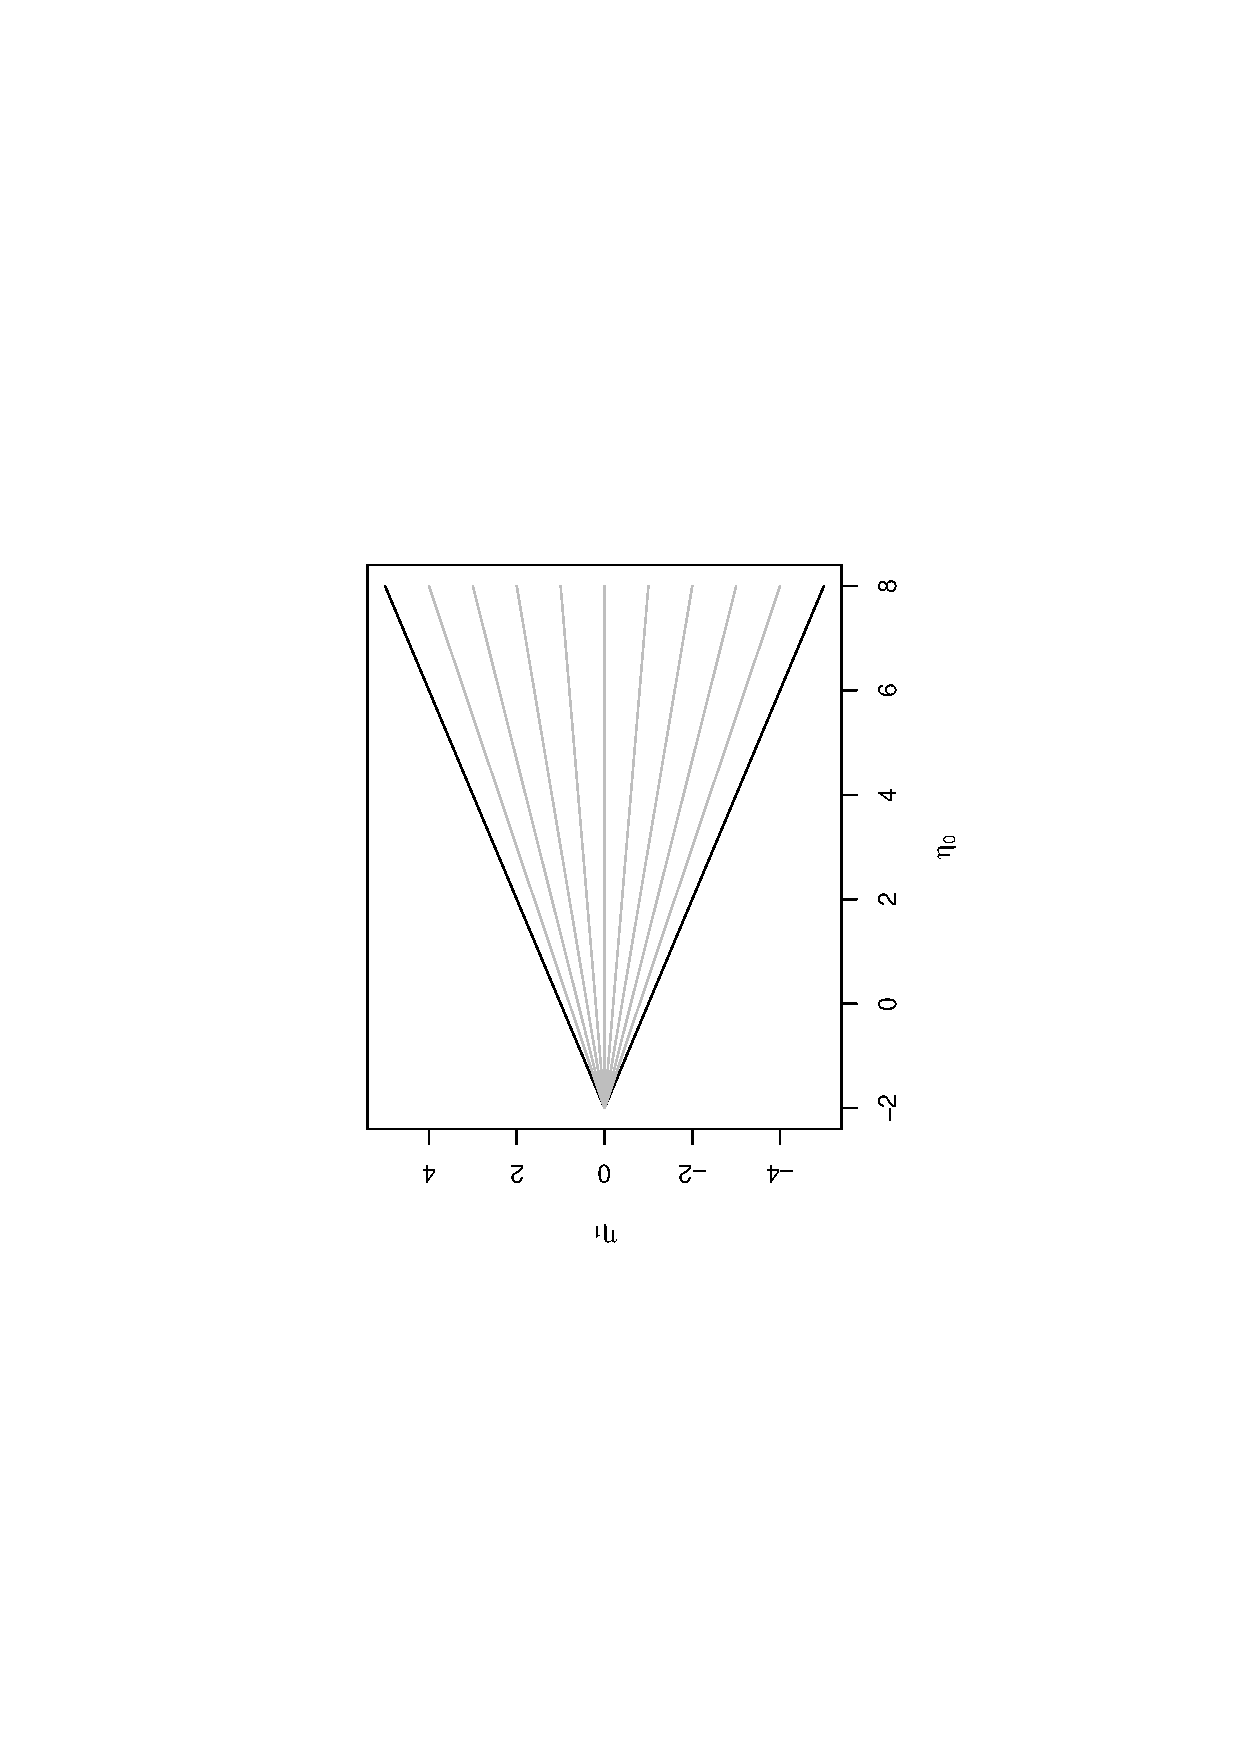
\includegraphics[trim = 80mm 45mm 80mm 60mm, clip, width=0.7\textwidth]{R/boatshape-domain}%
%}
\caption[Bounds for the domain of $\eta_0$ and $\eta_1$ for the Beta-Binomial model,
with rays of constant expectation for $y_c = \{0.1,0.2,\ldots,0.9\}$.]%
{Bounds for the domain of $\eta_0$ and $\eta_1$ for the Beta-Binomial model (black),
with rays of constant expectation for $y_c = \{0.1,0.2,\ldots,0.9\}$ (grey).}
\label{fig:boatshape-domain}
\end{figure}

As we wrote in Section~\ref{sec:concluding-outlook},
$\eta_1$ cannot have the convenient property of being equal to
the expectation of the mean sample statistic $\ttau(\x)$ (here, $s/n$),
as was the case for $y$.%
\footnote{For $\yz$, it holds that $\yz = \E\big[\E[\ttau(\x) \mid \psi] \mid \nz, \yz\big]$,
as mentioned in Section~\ref{sec:regularconjugates}.}
However, from \eqref{eq:trafotony} we can derive that coordinates $(\eta_0,\eta_1) \in \Eta$ satifying
\begin{align}
\label{eq:raysofconstantexpectation}
\eta_1 = f(\eta_0) &= (\eta_0 + 2)(y_c - \frac{1}{2}) 
\end{align}
will have a constant expectation $y_c$.
The domain $\Eta$, and these \emph{rays of constant expectation} emanating from the coordinate $(-2,0)$,
are depicted in Figure~\ref{fig:boatshape-domain}.

\subsection{The Boatshape}
\label{sec:boatshape-2}

When Mi\c{k}elis Bickis presented this parametrisation of conjugate priors at a talk,
both Frank Coolen and the author of this thesis had independently the same basic idea
for a set shape that allows for both \pdc\ sensitivity
%and gives `bonus precision' if prior and data agree especially well,
and more precise inferences in case of strong prior-data agreement.
The basic idea for this shape is described informally below,
while a suggestion for a parametrisation of such a shape is described and discussed
in the later subsections.

\subsubsection{Informal Rationale for Boat-Shaped Parameter Sets}
\label{boatshape-rationale}

In the parametrisation in terms of $(\nz,\yz)$ and $(\nn, \yn)$,
posterior inferences become more precise,
because the stretch in the main parameter dimension $y$, denoted by $\Delta_y(\PN)$,
tends to $0$ for $n \to \infty$ (see the discussion in Section~\ref{sec:gbicp-properties-criteria}).
In the domain $\Eta$ as depicted in Figure~\ref{fig:boatshape-domain},
instead the rays of constant expectation fan out for growing $n$, %**move outwards to the right,
while a parameter set will retain its size in updating.
Increased precision in a posterior parameter set $\EN$, which is just
its prior counterpart $\EZ$ shifted to the right,
is given by the fact the more $\EN$ is located to the right,
the fewer rays of constant expectation $\EN$ will intercept.
Imprecision in terms of $\E\big[\E[\ttau(\x) \mid \psi] \mid \nn, \yn\big] = \yn$
can thus be imagined as the size of the `shadow' that a set $\EN$ casts
when considering a light source in $(-2,0)$ (the point from which the rays of constant expectation emanate).
In short, the smaller this shadow, the more precise the inferences.

In the context of the model from Section~\ref{sec:miksworld},
we will denote by $\ynl$ and $\ynu$ the bounds of this shadow,
i.e.,
\begin{align*}
\ynl &:= \min_{(\ezn,\eon) \in \EN} \yn = \min_{(\ezn,\eon) \in \EN} \frac{\eon}{\ezn+2} + \frac{1}{2}\,, \\
\ynu &:= \max_{(\ezn,\eon) \in \EN} \yn = \max_{(\ezn,\eon) \in \EN} \frac{\eon}{\ezn+2} + \frac{1}{2}\,,
\end{align*}
and we call the coordinates $\argmin_{(\eta_0,\eta_1) \in \EN} \yn$ and $\argmax_{(\eta_0,\eta_1) \in \EN} \yn$
the \emph{touchpoints} of $\EN$ responsible for the shadow $[\ynl, \ynu]$.
Mutatis mutandis, the same definitions can be made for the prior set $\EZ$.

Due to the fanning out of rays, most shapes for $\EZ$ will lead to decreasing imprecision for increasing $n$.
Indeed, models of type~(\ref{enum:modeltypes-a}) from Section~\ref{sec:basicsetting},
where $\PZ = \nz \times [\yzl, \yzu]$,
are represented here again by a line segment $\EZ = \ezz \times [\eozl,\eozu]$,
such that the posterior touchpoints are, for any $s$ and $n$, $(\ezn,\eonl)$ and $(\ezz,\eonu)$,
where $\eonl$ and $\eonu$ are the updated versions of $\eozl$ and $\eozu$, respectively.
Due to \eqref{eq:eta-update}, it holds that $\eonu-\eonl = \eozu-\eozl$;
therefore, imprecision decreases here because a line segment of fixed size
will cast a smaller shadow when further to the right,
as illustrated in Figure~\ref{fig:boatshape-vertical}.

\begin{figure}  %trim=l b r t
\centering
%\fbox{%
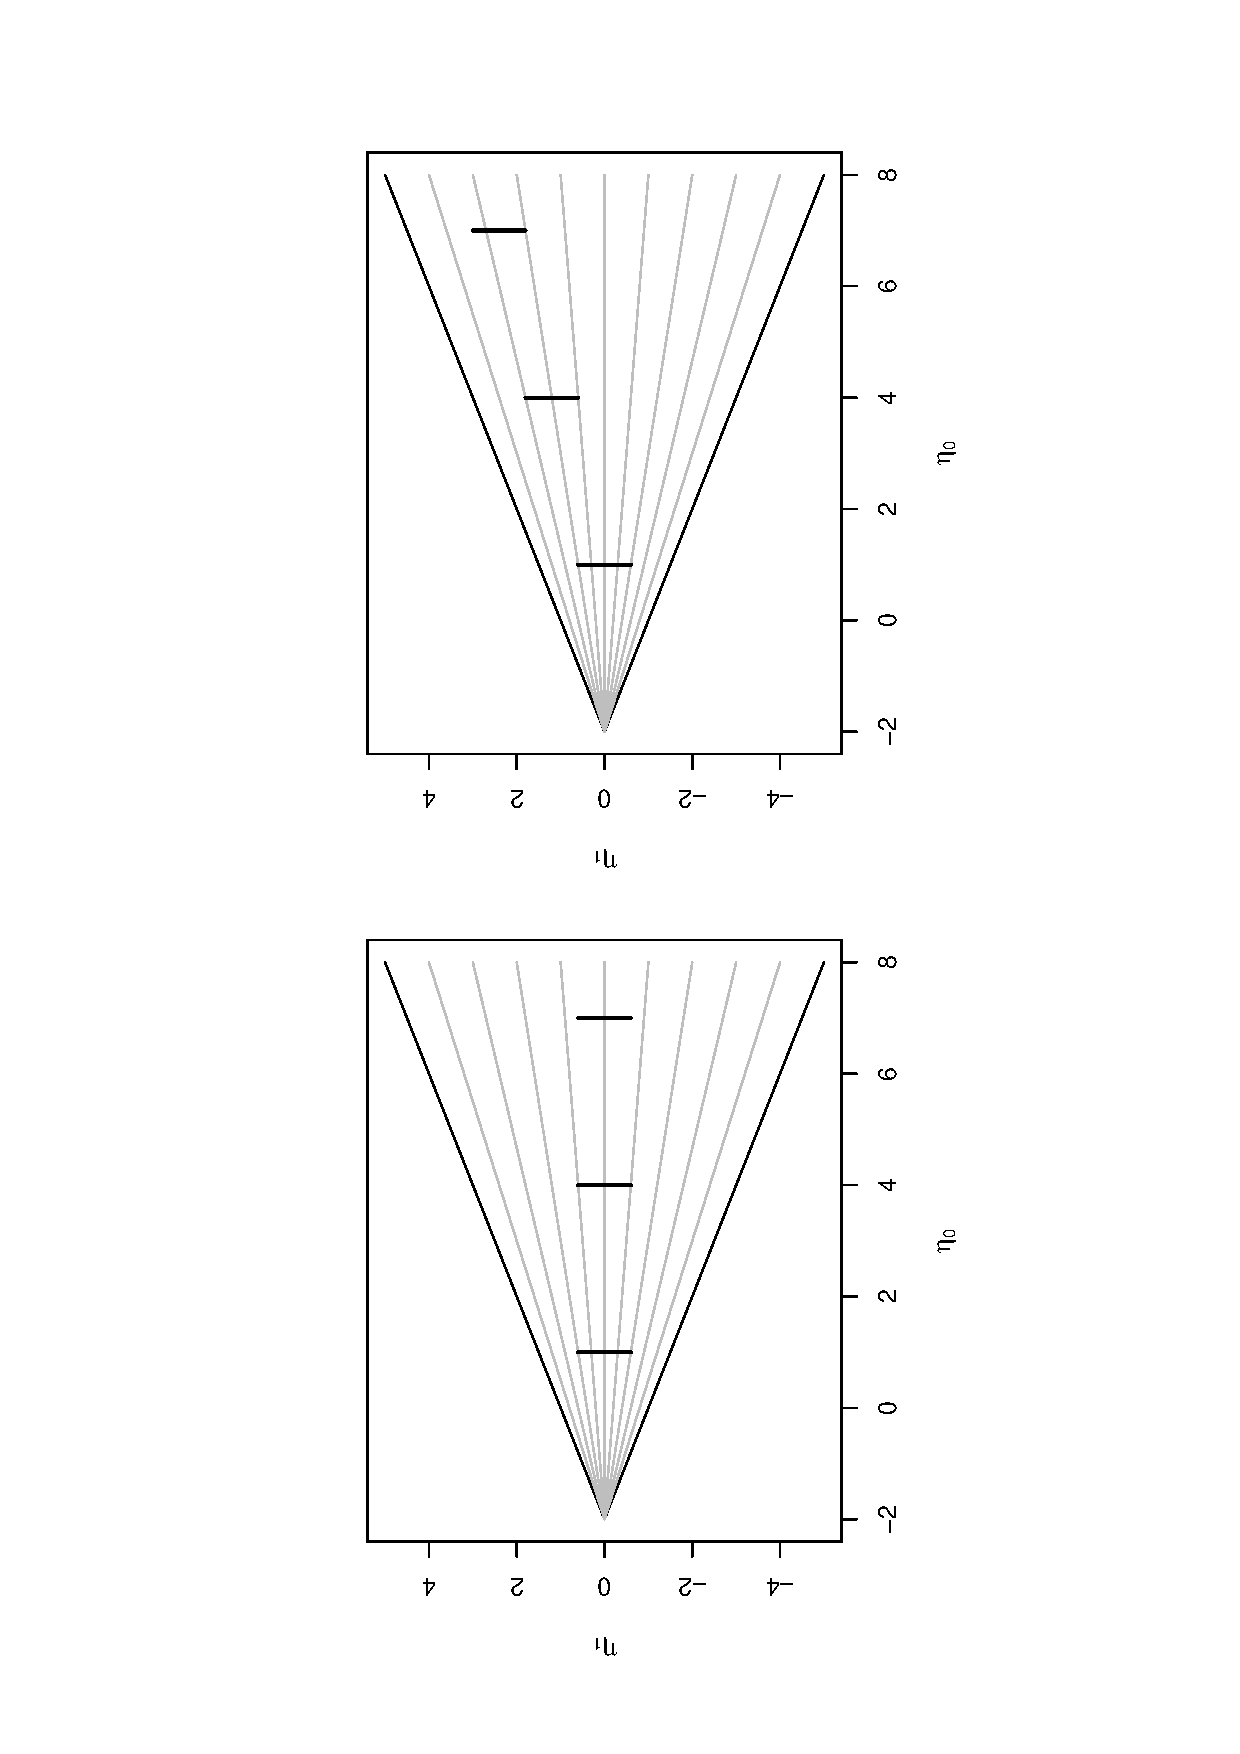
\includegraphics[trim = 15mm 45mm 25mm 60mm, clip, width=\textwidth]{R/boatshape-vertical}%
%}
\caption[Line segment parameter set $\EZ$ %
and respective posterior sets for $s/n=0.5$ and $s/n=0.9$.]%
{Parameter set $\EZ = \ezz \times [\text{\underline{$\eta$}${}_1\uz$},\eozu]$ and respective posterior sets $\EN$
for $s/n=0.5$ (left) and $s/n=0.9$ (right). Note that all sets have the same size,
imprecision decreasing only through their position on the $\eta_0$ axis.}
\label{fig:boatshape-vertical}
\end{figure}

For \pdc\ sensitivity, we need shapes that cover a range of $\eta_0$ values,
for the same reasons as in the framework of Section~\ref{sec:basicsetting},
where only sets with a range of $\nz$ values offered this property.
Sets that are elongated along the rays of constant expectation
will behave here similar to the rectangular shapes of Section~\ref{sec:basicsetting}.
When shifted along its respective ray of constant expectation,
imprecision will be reduced as the shadow of the set will become smaller just as described above for line segments.
When such a shape is instead shifted away from its ray of constant expectation,
imprecision will be increased, as a prolonged shape that is now turned away from its ray 
will cast a larger shadow.%
\footnote{This will become clear from the depiction of boatshape sets in Figure~\ref{fig:boatshape-posterior-mik}.} 

A set $\EZ$ allowing for less imprecison in case of strong prior-data agreement
must also be able to cast a smaller shadow if the update shift goes into the direction of its ray,
%of $s/n$ according the information,
but we will enhance this effect by considering now also the properties
of the canonical posteriors the coordinates of $\EN$ represent.

We have seen that for the conjugate distributions themselves,
$\nz$ is generally a parameter determining the spread of the distribution
(e.g., in the Normal-Normal model (see Section~\ref{sec:norm-norm}), $\nz$ was the inverse variance),
such that we will have more precise inferences if the shadow bounds $\ynl$ and $\ynu$
are attained at higher values of $\eta_0$, leading to lower variances in the
`critical' distributions at the boundary of the posterior expectation interval $[\ynl,\ynu]$.
For this to happen, we need a shape for which the touchpoints responsible for $\ynl$ and $\ynu$
are attained at higher values of $\eta_0$ in case of strong prior-data agreement.
Shapes that accomplish this must have a curvature along their length in the direction
of the constant rays of expectation.
The shape we suggest thus looks like a bullett, or like a boat with a transom stern
(see Figure~\ref{fig:boatshape-prior}).

\subsubsection{Basic Definition}
\label{sec:basicdefboat}

We will now present a parametrisation for such a boat-shaped parameter set $\EZ$.
To keep things simple, we will consider here and in the follwing only prior sets
that are symmetric around the $\eta_0$ axis, i.e., centered around $y_c = 0.5$,
expressing prior the information that we deem a fraction of successes of $\frac{s}{n} = \frac{1}{2}$
as the most probable.%
\footnote{The general case of sets $\EZ$ with central ray $y_c \neq 0.5$
is discussed informally in *****}

For the contours of $\EZ$, we suggest an exponential function as the functional form,
where the `prow' of the set is located at $(\ezl, 0)$.
The lower and the upper contour $\czl(\eta_0)$ and $\czu(\eta_0)$ are defined as
\begin{align*}
\czl(\eta_0) &= -a \left( 1 - e^{-b(\eta_0 - \ezl)} \right)\,, \\
\czu(\eta_0) &= \phantom{-}%
                 a \left( 1 - e^{-b(\eta_0 - \ezl)} \right)\,, 
\end{align*}
where $a$ and $b$ are parameters controlling the shape.
We will also need the respective derivations with respect to $\eta_0$, given by
\begin{align*}
\frac{d}{d\eta_0} \czl(\eta_0) &= -ab e^{-b(\eta_0 - \ezl)}\,, \\
\frac{d}{d\eta_0} \czu(\eta_0) &= \phantom{-}%
                                   ab e^{-b(\eta_0 - \ezl)}\,.
\end{align*}

For this basic situation, given the parameters $\ezl$, $\ezu$, $a$, and $b$,
$\EZ$ is thus defined as
\begin{align}
\label{eq:basicset}
\EZ =
\{(\eta_0,\eta_1) \colon \ezl \le \eta_0 \le \ezu, \czl(\eta_0) \le  \eta_1 \le \czu(\eta_0) \}\,.
\end{align}
A prior boatshape set with $\ezl=1$, $\ezu=6$, $a=2$, and $b=0.8$ is depicted in Figure~\ref{fig:boatshape-prior},
where the left graph shows this set as defined in terms of $(\eta_0,\eta_1)$,
and the right graph shows the set from the left transformed into the space $\N \times \Y$.

\begin{figure}  %trim=l b r t
\centering
%\fbox{%
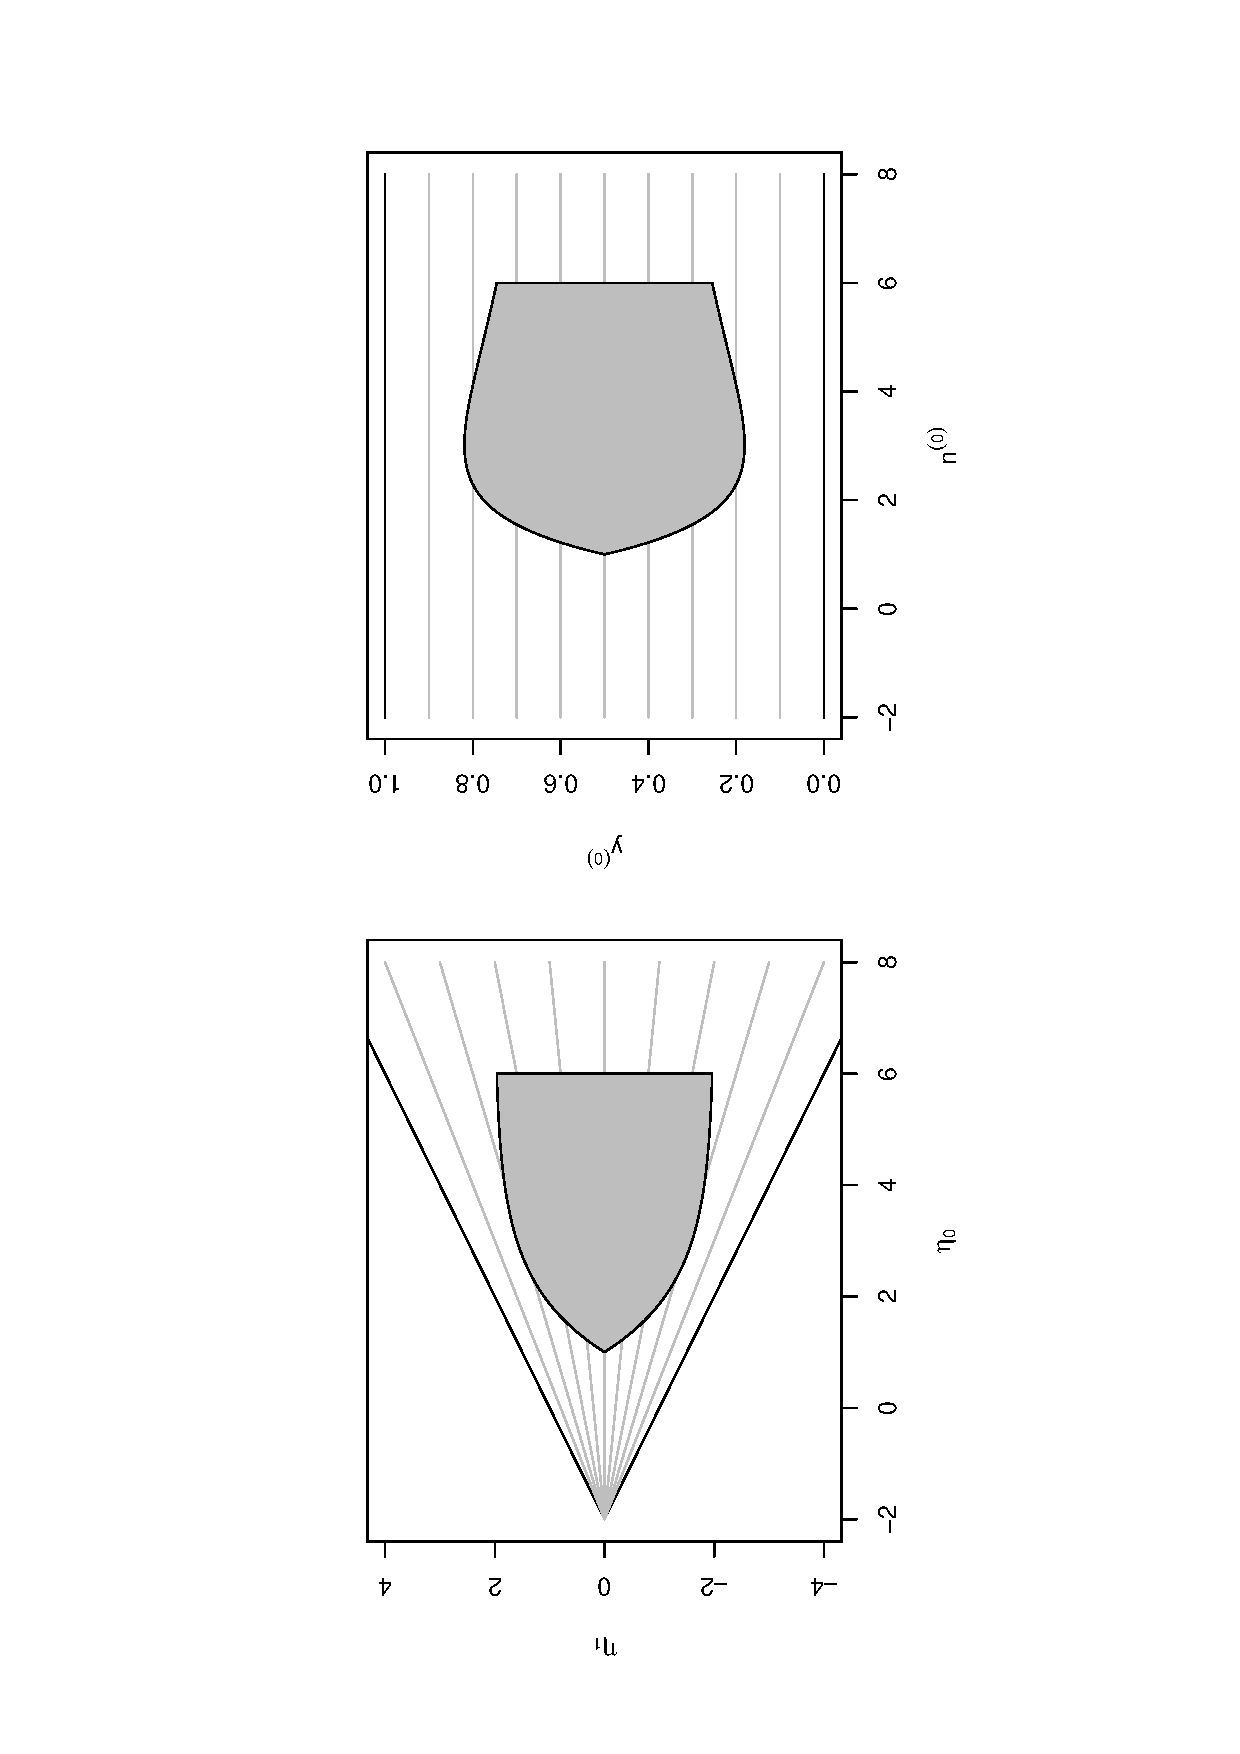
\includegraphics[trim = 15mm 45mm 25mm 60mm, clip, width=\textwidth]{R/boatshape-prior}%
%}
\caption[Boatshape prior set in the parametrisation via $(\eta_0,\eta_1)$ and via $(\nz,\yz)$.]%
{Boatshape prior set in the parametrisation via $(\eta_0,\eta_1)$ (left) and via $(\nz,\yz)$ (right),
with parameters $\ezl=1$, $\ezu=6$, $a=2$, and $b=0.8$.}
\label{fig:boatshape-prior}
\end{figure}


We have as yet no good formal description for the role of the parameters $a$ and $b$. %that,
%togeher with $\ezl$ and $\ezu$, define the boat-set (see Section~\ref{sec:basicdefboat} below).
Informally, $a$ determines the half-width of the set;
the width, i.e., the size in the $\eta_1$ dimension, would be $a$ if $\ezu \to \infty$.
$b$ instead determines the `bulkyness' of the shape.
Together with $\ezl$, $a$ and $b$ determine the prior interval for the expected success probability $[\yzl, \yzu]$.
For fixed $\ezl$ and $a$, increasing $b$ leads to a wider prior expectation interval.
For $[\yzl, \yzu]$, the choice of $\ezu$ is irrelevant.%
\footnote{$\ezu$ plays only a role in determining when the `unhappy learning' phase starts
(see end of Section~\ref{sec:generalupdate}).}


\begin{figure}  %trim=l b r t
\centering
%\fbox{%
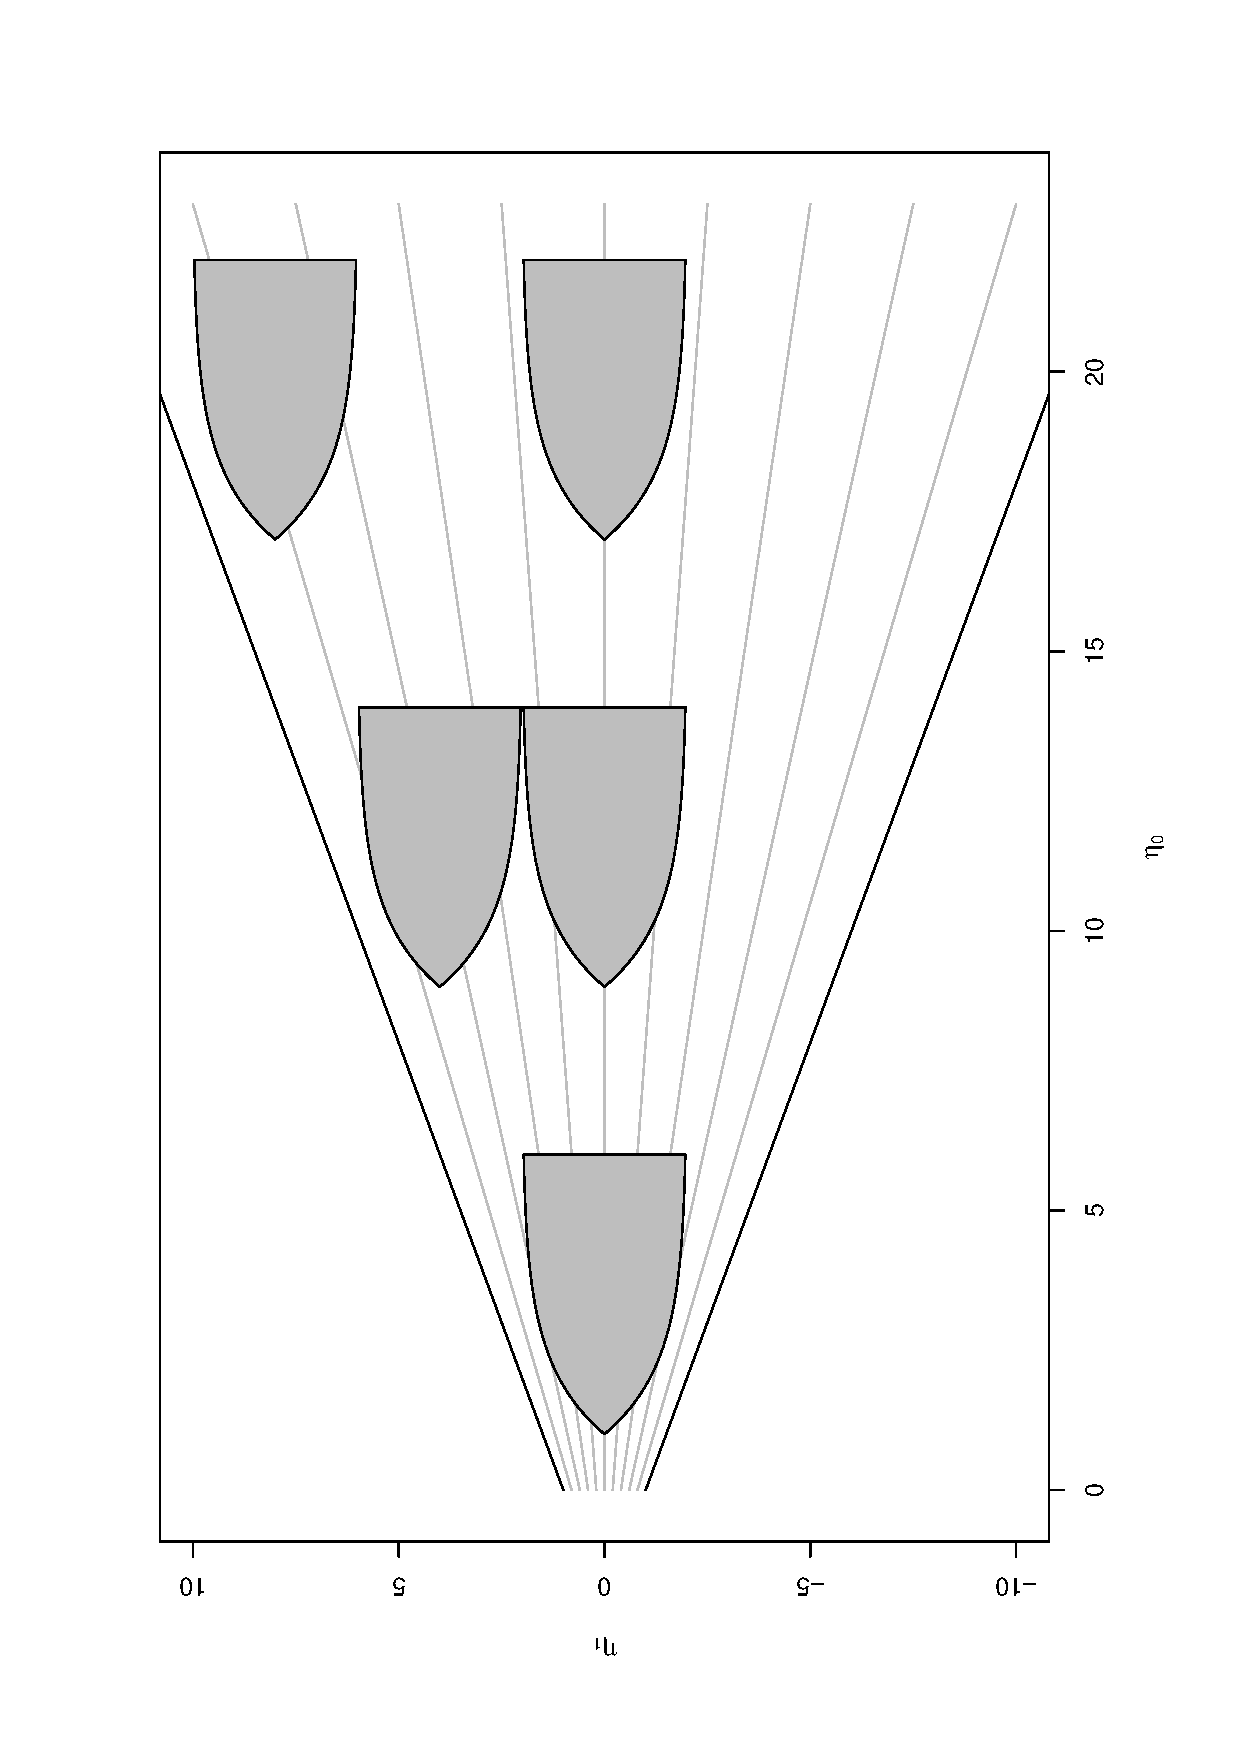
\includegraphics[trim = 20mm 35mm 30mm 45mm, clip, width=\textwidth]{R/boatshape-posterior-mik}%
%}
\caption[Boatshape prior and posterior sets for data in accordance and in conflict with the prior.]%
{Boatshape prior and posterior sets for data in accordance and in conflict with the prior.
The prior set is the same as in Figure~\ref{fig:boatshape-prior}.
While the posterior sets for $\frac{s}{n}=0.5$ move along the ray for $y_c=0.5$,
the posterior sets for $\frac{s}{n}=1$ are shifted away from the ray for $y_c=0.5$,
resulting in increased posterior imprecision.
Note that lower and upper touchpoints are in the middle of the contour
for the prior and the posterior resulting for data $\frac{s}{n}=\frac{4}{8}$,
while at least one touchpoint is at the end for all other sets.
(see also Figure~\ref{fig:boatshape-posterior-normal}).}
\label{fig:boatshape-posterior-mik}
\end{figure}


\begin{figure}  %trim=l b r t
\centering
%\fbox{%
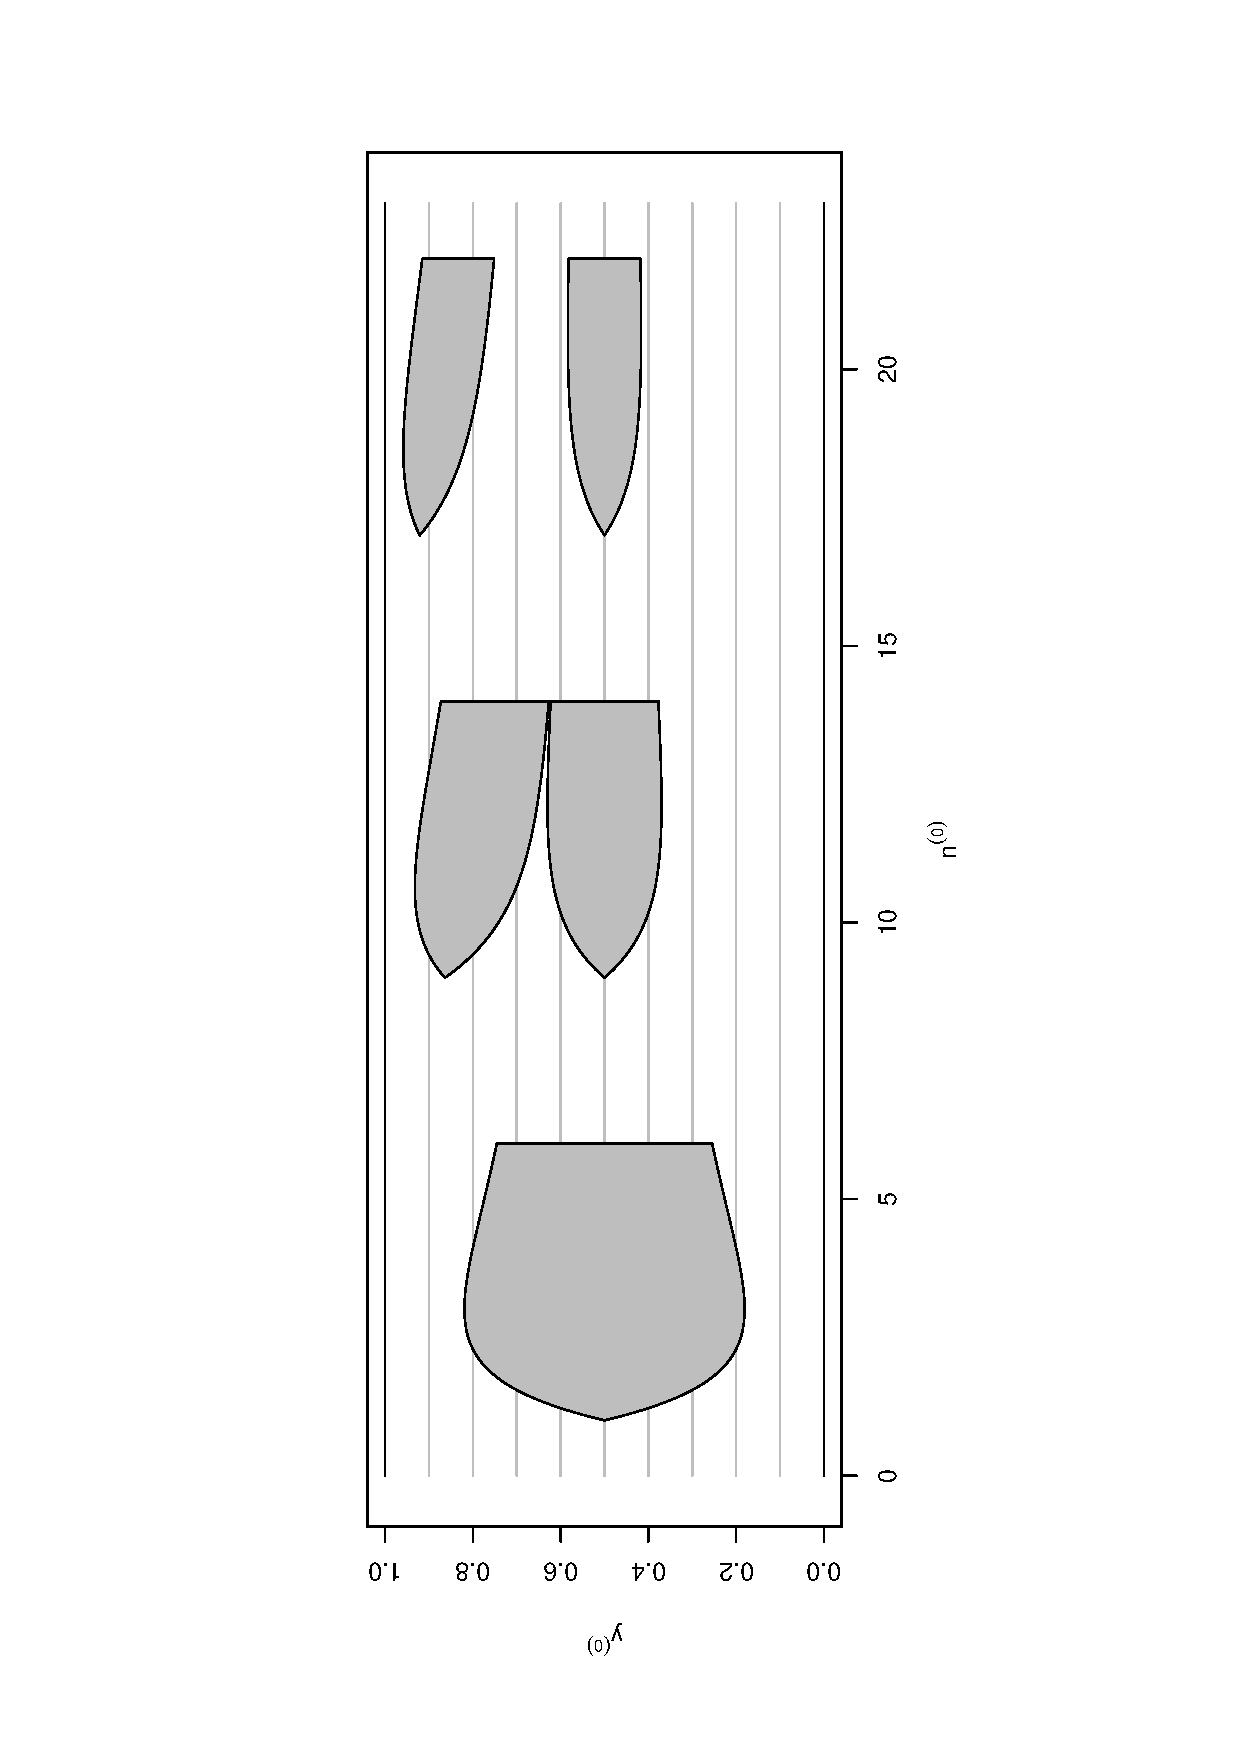
\includegraphics[trim = 15mm 45mm 25mm 60mm, clip, width=\textwidth]{R/boatshape-posterior-normal}%
%}
\caption[Boatshape prior and posterior sets from Figure~\ref{fig:boatshape-posterior-mik} in the parametrisation via $(\nz,\yz)$.]%
{Boatshape prior and posterior sets from Figure~\ref{fig:boatshape-posterior-mik} in the parametrisation via $(\nz,\yz)$.
Note that in the strong prior-data agreement case,
posteriors based on a rectangular set with the same prior main parameter imprecision
would be larger than the ones depicted here, illustrating the extra gain in precision.}
\label{fig:boatshape-posterior-normal}
\end{figure}


\subsubsection{Finding the Touchpoints for the Basic Set}

In contrast to models discussed in Section~\ref{sec:generalmodel},
where $\yzl$ and $\yzu$ were at either ends of a set $\PZ$,
here, for a set \eqref{eq:basicset}, the touchpoints $\yzl$ and $\yzu$ 
are not necessarily at $\ezzl$ or $\ezzu$.
\footnote{See, e.g., the prior in Figure~\ref{fig:boatshape-prior}.}
Instead, the rays of constant expectation \eqref{eq:raysofconstantexpectation}
touching the parameter set must be determined to find $\yzl$ and $\yzu$.
To do this, the tangent equations for the lower and the upper contour function
depending on $\eta_0$ are determined.
As all rays of constant expectation pass through the point $(-2,0)$,
the tangent that passes through this point is determined by inserting this point
into the tangent equation, and the resulting equation is solved for $\eta_0$.
The resulting points $(\eta_0^u,\czu(\eta_0^u))$ resp.\ $(\eta_0^l,\czl(\eta_0^l))$
then give the touchpoints of the parameter set,
and can be transformed to $\yzl$ and $\yzu$ by using \eqref{eq:trafotony}.

As the basic set is symmetrical to the $\eta_0$ axis, $\eta_0^u = \eta_0^l$,
and it suffices to find, e.g., $\eta_0^u$, by considering the upper contour tangent.

We denote the tangent in contour point $(\eta_0,\czu(\eta_0))$ by
\begin{align*}
\ol{t}_{\eta_0}(x) &= dx + i\,,
\end{align*}
where $d = \frac{d}{d\eta_0} \czu(\eta_0)$ and
$i$ such that $\ol{t}_{\eta_0}(x)$ goes through the point $(\eta_0,\czu(\eta_0))$:
\begin{align*}
\ol{t}_{\eta_0}(x) &= dx + i \quad \equiv\\
\czu(\eta_0) &= \frac{d}{d\eta_0} \czu(\eta_0) \eta_0 + i \\
i &= \czu(\eta_0) -\frac{d}{d\eta_0} \czu(\eta_0) \eta_0 \\
  &= a - a e^{-b(\eta_0 - \ezl)} - \eta_0 ab e^{-b(\eta_0 - \ezl)} \\
  &= a - a (1 + b \eta_0) e^{-b(\eta_0 - \ezl)} \\
\Longrightarrow\quad
\ol{t}_{\eta_0}(x) &= ab e^{-b(\eta_0 - \ezl)} x + a - a (1 + b \eta_0) e^{-b(\eta_0 - \ezl)} \\
                   &= a - a \big(1 + b(\eta_0-x)\big) e^{-b(\eta_0 - \ezl)}
\end{align*}

Now, let us find the touchpoint $(\eta_0^u, \czu(\eta_0^u))$ whose tangent goes through $(-2,0)$, as this gives us $\yzu$.
We insert $(-2,0)$ into the tangent equation and solve for $\eta_0$.
\begin{align}
a - a \big(1 + b(\eta_0^u + 2)\big) e^{-b(\eta_0^u - \ezl)} &\stackrel{!}{=} 0 \nonumber\\
1 + b(\eta_0^u + 2) &\stackrel{!}{=} e^{b(\eta_0^u - \ezl)} \label{eq:eta0u}
\end{align}
This equation has only one solution for $\eta_0^u > \ezl$, that is,
however, not available in closed form.

As a general rule, the nearer $\eta_0^u$ is to $\ezl$, the larger $\frac{d}{d\eta_0} \czu(\eta_0^u)$,
that is, $\yzu$ %the upper expected value for the prior set
is more away from $\frac{1}{2}$.
Here, this means that the larger $\eta_0^u$, the more imprecise is the prior parameter set.

\subsubsection{Strong Prior-Data Agreement Property}
\label{sec:spda-property}

For a prior parameter set $\EZ = \ezz \times [\eozl,\eozu]$
%, with $\eta_0 = \ezz$ fixed and $\eta_1$ varying in an interval $[\eol, \eou]$
symmetric around $0$,
the prior upper expected value $\yzu$
results from the transformation \eqref{eq:trafotony} of the point $(\ezz,\eozu)$.
The posterior upper expected value $\ynu$,
given data that coincide especially well with the prior,
i.e., data with $s = \frac{n}{2}$, will then be found at the point $(\ezz+n,\eozu)$,
because in this case, the set does not move in the vertical ($\eta_1$) direction.
As $\yz$ is decreasing in $\eta_0$ and $\eta_1$ is constant, $\ynu$ %the posterior upper expected value
will be lower than $\yzu$, i.e., imprecision is reduced.

Imprecision is, however, even more strongly reduced for the boatshape parameter set \eqref{eq:basicset}.
Say, we define the prior parameter set such that the prior upper touchpoint
is at the $\eta_0$ coordinate $\eta_0^u = \ezz$.
For this shape, the $\eta_0$ coordinate for the posterior upper touchpoint ${\eta_0^u}\un$
will be  larger than the updated $\ezz$, i.e., ${\eta_0^u}\un > \ezz + n$ (as will be shown below), and thus $\ynu$ is lower.
Although the $\eta_1$ coordinate will be slightly larger at the point $({\eta_0^u}\un, \ol{c}({\eta_0^u}\un))$
as compared to the point $(\ezz+n,\eozu)$, the corresponding $\ynu$ is still lower,
as it holds that
\begin{align*}
\frac{d}{d\eta_0} \ol{c}({\eta_0^u}\un) < \frac{d}{d\eta_0} \ol{c}(\ezz + n)
\end{align*}
because $\frac{d}{d\eta_0} \ol{c}(\eta_0)$ is decreasing in $\eta_0$,
and a smaller slope for the tangent through $(-2,0)$ is equivalent to a lower $\ynu$.
This is the desired reduction in imprecision for the case of strong prior-data agreement,
also depicted exemplarily in Figures~\ref{fig:boatshape-posterior-mik} and \ref{fig:boatshape-posterior-normal}.

The property ${\eta_0^u}\un > \ezz + n$ of the boatshape set will be shown below.
Due to symmetry of prior and posterior parameter shape around the $\eta_0$ axis,
${\eta_0^u}\un = {\eta_0^l}\un$, i.e.,
the touchpoint at the upper contour (giving $\ynu$) is equal to
the touchpoint at the lower contour (giving $\ynl$),
and thus, the argument formulated in terms of ${\eta_0^u}\un$ holds also for ${\eta_0^l}\un$.

The upper exponential contour for the posterior boatshape,
updated with $s = \frac{n}{2}$, has its `prow' now at $(\ezl + n, 0)$,
and is defined by the function
\begin{align*}
\ol{c}(\eta_0) &= a \left( 1 - e^{-b(\eta_0 - n -\ezl)} \right) \\
\frac{d}{d\eta_0} \ol{c}(\eta_0) &= ab e^{-b(\eta_0 - n - \ezl)} \,.
\end{align*}

The tangent in contour point $(\eta_0,\ol{c}(\eta_0))$ is
\begin{align*}
\ol{t}_{\eta_0}(x) &= a - a \big(1 + b(\eta_0-x)\big) e^{-b(\eta_0 - n - \ezl)} \,.
\end{align*}

Again, we insert $(-2,0)$ into this tangent equation and solve for $\eta_0$.
\begin{align}
a - a \big(1 + b({\eta_0^u}\un + 2)\big) e^{-b({\eta_0^u}\un - n - \ezl)} &\stackrel{!}{=} 0 \nonumber\\
1 + b({\eta_0^u}\un + 2) &\stackrel{!}{=} e^{b({\eta_0^u}\un - n - \ezl)} \,.\label{eq:eta0uposterior}
\end{align}
We compare now \eqref{eq:eta0uposterior} to \eqref{eq:eta0u} and conclude
that indeed ${\eta_0^u}\un > \ezz + n$.

\begin{figure}
\centering
\begin{tikzpicture}[pin distance=1cm]
\node (0,0) {%\fbox{% %trim=l b r t
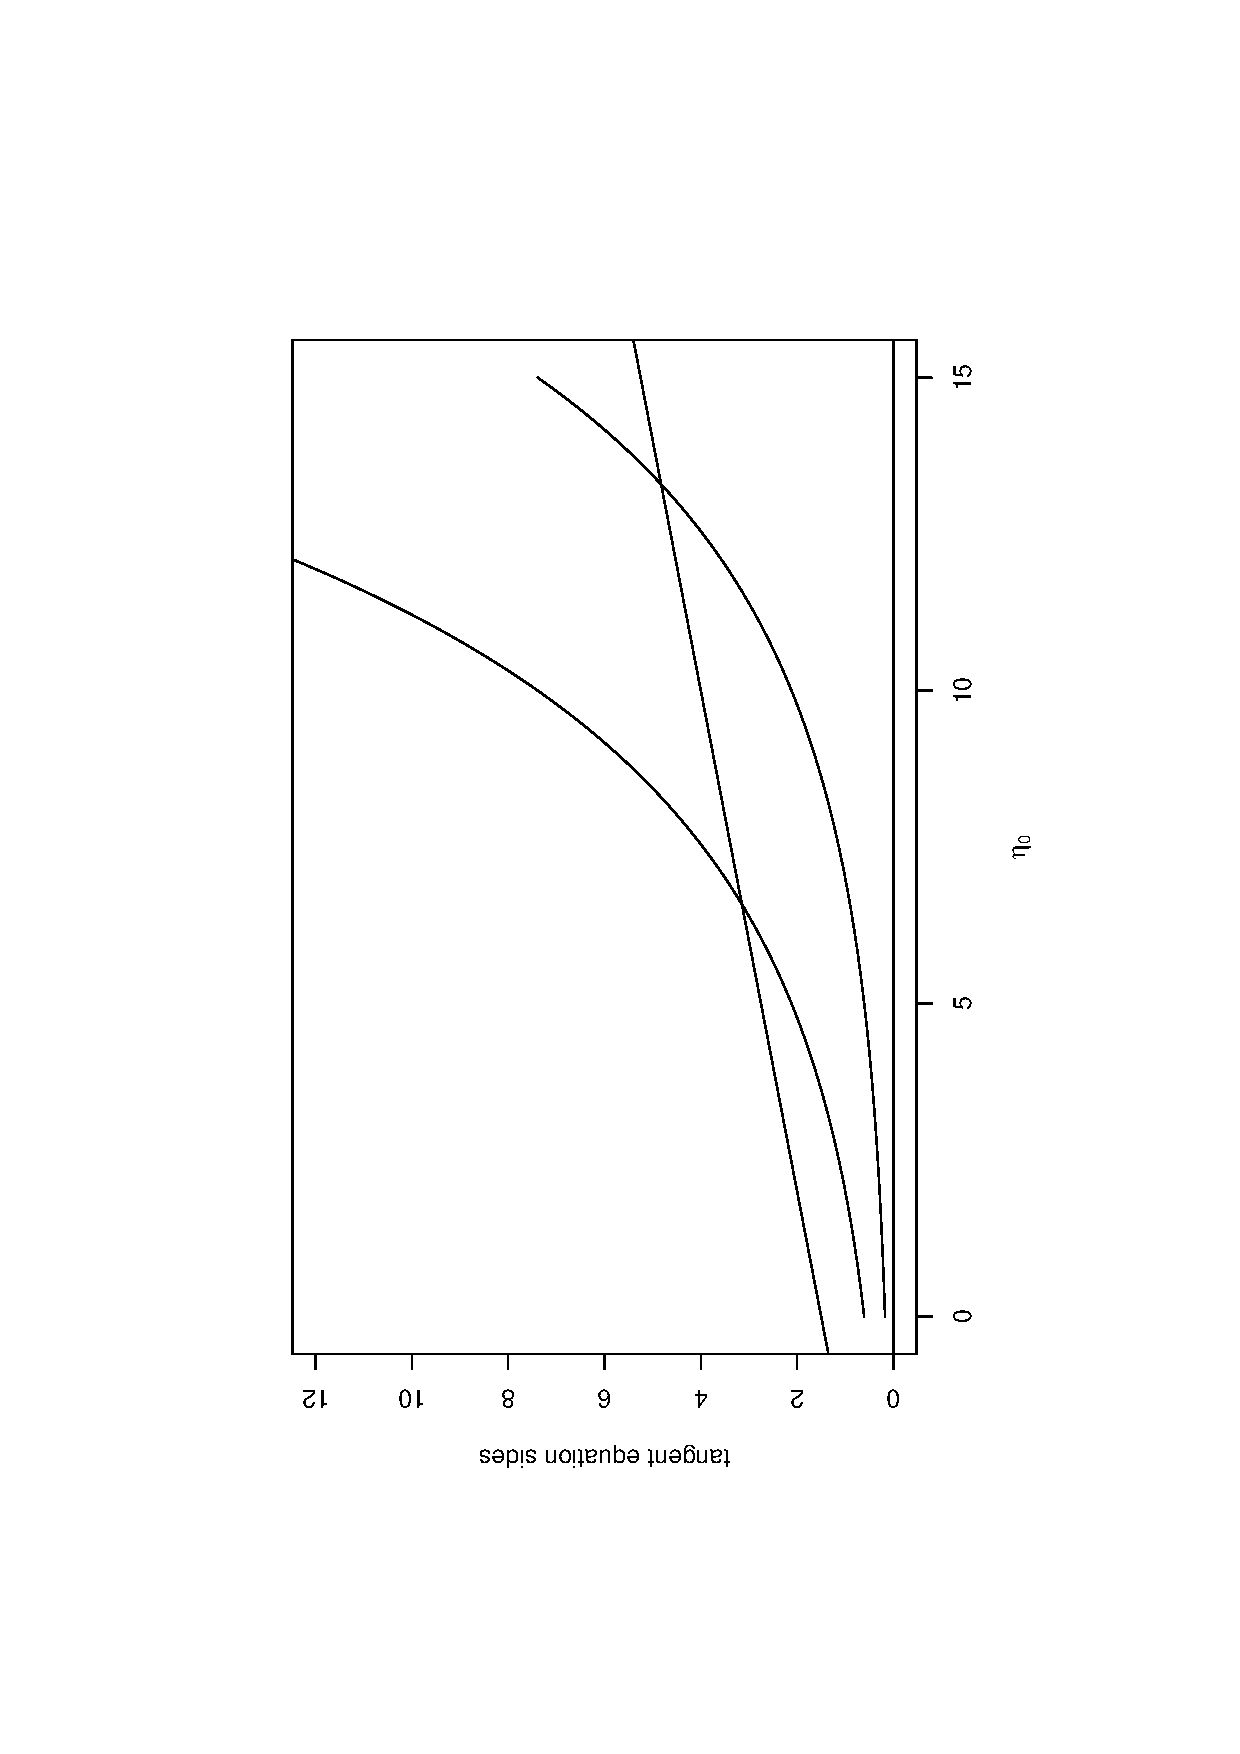
\includegraphics[trim = 45mm 35mm 45mm 45mm, clip, width=\textwidth]{R/prior-vs-posterior-eta0u}%
};
\coordinate (x1) at (-0.35,-1.21);
\draw (x1) circle (2.5pt);
\coordinate [pin=below:${\eta_0^u}\uz$] (a1) at (-0.35,-3.24);
\draw[dashed] (x1) -- (a1);
\coordinate (x2) at ( 5.2 ,-0.15);
\draw (x2) circle (2.5pt);
\coordinate [pin=-70:${\eta_0^u}\un$] (a2) at ( 5.2,-3.24);
\draw[dashed] (x2) -- (a2);
\coordinate (x1n) at (3.8,-1.21);
%\draw (x1n) circle (2.5pt);
%\coordinate [label=below:${\eta_0^u}\uz + n$] (a1n) at (3.8,-3.5);
\coordinate [pin=below:${\eta_0^u}\uz + n$] (a1n) at (3.8,-3.24);
\draw[dashed] (x1) -- (x1n) -- (a1n);
\end{tikzpicture}
\caption{Illustration for the argument that ${\eta_0^u}\un > {\eta_0^u}\uz + n$.}
\label{fig:spda1}
\end{figure}

In Figure~\ref{fig:spda1}, the two exponential graphs have the same curvature,
the right one is the same as the left, only being shifted to the right by $n$.
The value of $\ezz + n$, defined as the abscissa of the intersection of the left exponential and the linear function,
being shifted to the right by $n$, would thus be on the right exponential curve.
Because ${\eta_0^u}\un$ results from the intersection of the right exponential curve and the linear function,
it is necessarily larger than ${\eta_0^u}\uz + n$, as the linear function is increasing.


\subsubsection{General Update with \texorpdfstring{$s > \frac{n}{2}$}{s > n/2}}
\label{sec:generalupdate}

Let us now consider updating of the basic boatshape \eqref{eq:basicset}. %symmetric around the $\eta_0$ axis,
As the prior set is symmetric around the $\eta_0$ axis,
the touchpoints are located at the same $\eta_0$ coordinate,
the resulting $\yzl$ and $\yzu$ having the same distance to $0.5$.

According to \eqref{eq:eta-update},
$\eta_0$ coordinates are incremented by $n$, while
$\eta_1$ coordinates are incremented by $s+\frac{n}{2}$.
That is, if $s \neq \frac{n}{2}$, the updated set is no longer symmetric around the $\eta_0$ axis,
such that we must consider the lower and upper contours separately.

The upper and lower contours and their respective derivatives for the updated boatshape set are now
\begin{align*}
\ol{c}(\eta_0)                   &= s - \frac{n}{2} + a - a e^{-b(\eta_0 - n - \ezl)} \,,\\
\frac{d}{d\eta_0} \ol{c}(\eta_0) &=                      ab e^{-b(\eta_0 - n - \ezl)} \,,\\
\ul{c}(\eta_0)                   &= s - \frac{n}{2} - a + a e^{-b(\eta_0 - n - \ezl)} \,,\\
\frac{d}{d\eta_0} \ul{c}(\eta_0) &=                     -ab e^{-b(\eta_0 - n - \ezl)} \,.
\end{align*}
The upper and lower tangents in contour point $(\eta_0,c(\eta_0))$ are now given by
\begin{align*}
\ol{t}_{\eta_0}(x) &= s - \frac{n}{2} + a - a \big(1 + b(\eta_0-x)\big) e^{-b(\eta_0 - n - \ezl)} \,,\\
\ul{t}_{\eta_0}(x) &= s - \frac{n}{2} - a + a \big(1 + b(\eta_0-x)\big) e^{-b(\eta_0 - n - \ezl)} \,.
\end{align*}
Inserting again $(-2,0)$, we get the equations defining the $\eta_0$ coordinates
${\eta_0^u}\un$ and ${\eta_0^l}\un$
that give us $\ynu$ and $\ynl$, respectively:
\begin{align}
%s - \frac{n}{2} + a - a \big(1 + b(\eta_0^u + 2)\big) e^{-b(\eta_0^u - n - \ezl)} &\stackrel{!}{=} 0 \nonumber\\
\label{eq:eta0u-general}
\frac{a}{s - \frac{n}{2} + a} \big(1 + b(\eta_0^u + 2)\big) &\stackrel{!}{=} e^{b(\eta_0^u - n - \ezl)} \,,\\
\label{eq:eta0l-general}
\frac{a}{\frac{n}{2} -s  + a} \big(1 + b(\eta_0^u + 2)\big) &\stackrel{!}{=} e^{b(\eta_0^u - n - \ezl)} \,.
\end{align}

We see thus that the picture from Figure~\ref{fig:spda1} holds here as well,
except that the linear function (left hand side of equations
\eqref{eq:eta0u-general} and \eqref{eq:eta0l-general}) is changed in slope and intercept by a factor.
(Equivalently, we can consider it to be rotated around the root $-2-\frac{1}{b}$.)
For $s=\frac{n}{2}$, this factor is 1 for both the lower and the upper touchpoint,
resulting in the situation of strong prior-data agreement as considered in Section~\ref{sec:spda-property},
where ${\eta_0^u}\un = {\eta_0^l}\un$ moved to the right.

Due to symmetry, we will consider the case $s > \frac{n}{2}$ only 
to describe ${\eta_0^u}\un$ and ${\eta_0^l}\un$.






--------------------------------


possible to put information in near-noninformative set $\EZ$!

***As our preliminary studies show some very appealing results in case of the Beta-Binomial model,
for which a possible parametrisation of our shape is discussed in Section~\ref{sec:boatshape},
we are confident that these encouraging results also hold for the Normal-Normal model
and in the general case of canonical conjugates.
A joint publication of Mi\c{k}elis Bickis, Frank Coolen and the author of this thesis is planned
that will elaborate these findings in more detail.





%

  \end{appendix}


  \backmatter

  %\include{bibliographie}
  %\addcontentsline{toc}{chapter}{\protect Bibliography}

  %\bibliographystyle{plainnat}
  %\bibliography{bib/eigene,bib/itip-refs,bib/other-refs}
  %\markboth{Bibliography}{Bibliography}
  
  %\printbibliography[heading=bibnumbered]

  \printbibliography
  \addcontentsline{toc}{chapter}{\protect Bibliography}

%  \markboth{Eidesstattliche Versicherung}{Eidesstattliche Versicherung}
%  \addcontentsline{toc}{chapter}{\protect Eidesstattliche Versicherung}


%\selectlanguage{ngerman}
\chapter*{Eidesstattliche Versicherung}

Hiermit erkläre ich an Eides statt, dass diese Dissertation von mir
selbstständig und ohne unerlaubte Beihilfe angefertigt ist.\\[3ex]

München, den 14.~August 2013\\[2ex]
\hspace*{0.5\textwidth} {\small Gero Walter}


\selectlanguage{english}


%  \include{lebenslauf}


\end{document}
